%% Auteur: Simon-Pierre Boucher, Université Laval, Chapitre 1 : thèse de doctorat

\documentclass[12pt]{article}

\usepackage{amssymb,amsmath,amsfonts,eurosym,geometry,ulem,graphicx,caption,color,setspace,comment,footmisc,pdflscape,subfigure,array,hyperref}
\usepackage{rotating}
\usepackage{multirow}
\usepackage{tabularx}
\usepackage{booktabs}
\usepackage{lscape}
\usepackage[dvipsnames]{xcolor}
\definecolor{mypink1}{rgb}{0.858, 0.188, 0.478}
\usepackage{tablefootnote}
\usepackage{ragged2e}
\usepackage{nicematrix}
\usepackage{enumitem}
\usepackage{wasysym}
\usepackage{framed}
\usepackage{pgfgantt}
\usepackage{subfloat}
\usepackage{blindtext}
\usepackage{colortbl}
\usepackage{palatino}
\usepackage{mathpazo}
\usepackage[flushleft]{threeparttable}
\usepackage[margin=15pt,font=small,labelfont={bf,sf}]{caption}
\usepackage[semibold]{sourcesanspro}
\usepackage{sectsty}
\allsectionsfont{\sffamily}

\hypersetup{colorlinks,
citecolor=blue,
linkcolor=magenta
}

\usepackage{environ,atbegshi}
\makeatletter
\newif\ifAtEnd@DontShowMe
\newcommand*\contents@DontShowMe{}

\normalem

\doublespacing
\newtheorem{theorem}{Theorem}
\newtheorem{corollary}[theorem]{Corollary}
\newtheorem{proposition}{Proposition}
\newenvironment{proof}[1][Proof]{\noindent\textbf{#1.} }{\ \rule{0.5em}{0.5em}}

\newtheorem{hyp}{Hypothesis}
\newtheorem{subhyp}{Hypothesis}[hyp]
\renewcommand{\thesubhyp}{\thehyp\alph{subhyp}}

\usepackage{natbib}
\bibliographystyle{chicago}%abbrvnat
\setcitestyle{authoryear,open={(},close={)}} %Citation-related commands
\geometry{left=1.0in,right=1.0in,top=1.0in,bottom=1.0in}

\singlespacing
\title{\textbf{Has financialization changed the impact\\ of macroeconomic announcements?}}


\author{Simon-Pierre Boucher\footnote{PhD student in finance, Université Laval, Quebec City QC Canada G1V 0A6, email:   \texttt{simon-pierre.boucher.1@ulaval.ca}}\and Marie-H{\'e}l{\`e}ne Gagnon\footnote{Professor of Finance and Research Fellow, CRREP, Université Laval, email: \texttt{marie-helene.gagnon@fsa.ulaval.ca}}\and Gabriel J. Power\footnote{IG Wealth Management Chairholder, Professor of Finance and Research Fellow, CRREP and CRIB, Université Laval, email:   \texttt{gabriel.power@fsa.ulaval.ca}}}

\date{\today}
\begin{document}
\begin{titlepage}
\maketitle

\singlespacing

\begin{abstract}
\noindent 
We investigate, using high-frequency data, how financialization has changed the impact of macroeconomic announcements on commodity futures returns and volatility. We find that greater financialization dampens the impact of macroeconomic release surprises on commodity markets, as measured by price drift and volatility changes. Moreover, financial participants improve liquidity and price discovery, while reducing volatility. Since traditional market participants prefer stability, our results suggest a beneficial impact of financialization. When we disaggregate the results, we find that the beneficial effects of greater financial participation are linked to money managers rather than swap dealers. 

\vspace{0.2in}
\noindent\textbf{Keywords:} commodities, energy, futures,  information diffusion, financialization, high-frequency, speculation, sustainable, commercial, institutional, volatility, macro, announcements, surprise, events.\\


\bigskip
\end{abstract}
\setcounter{page}{0}
\thispagestyle{empty}
\end{titlepage}
\pagebreak \newpage



\doublespacing

% Include section files
\section{Introduction} \label{sec:introduction}
%MH    MH     MH     il faut introduire des éléments du randr dans l'introduction sinon rien ne change et l'arbitre va penser qu'on a rien fait. 
Despite investment outflows in 2009 and 2014-2016,\footnote{These outflows are explained by the Great Recession and a global commodity slump, respectively.} commodities remain a popular asset class among non-traditional market participants such as hedge funds and index traders.  Indeed, 2022 may be a record year for commodity trading profit.\footnote{See, for example, the Wall Street Journal, September 9th 2022, ``Wall Street's Commodity Traders on Track to Break Profit Records''.} The financialization of commodities refers to important market and regulatory changes that have affected how commodities (futures, options, swaps and physicals) are traded by institutional and other non-traditional investors.  Financialization is controversial: Testimony given by \citet{masters2009testimony} to the Commodities Futures Trading Commission (CFTC) argued  that institutional investors disrupted commodity markets in the mid-2000s through the use of strategies intended for financial securities.\footnote{As we explain later, however, this claim has been challenged by empirical research \citep*{irwin2011index,irwin2012testing,irwin2012financialization}.} This paper investigates financialization in commodity markets through the lens of macroeconomic announcement releases.
 %MH    MH    MH    ici il manque une discussion sur comment on mesure la financiarisation.

Commodity financialization has coincided with a commodity bull cycle \citep*{humphreys2010great}, during which traditional market participants (i.e., those who produce or process the commodity) expressed fears that prices would be distorted from their fundamental values and that volatility increases would make hedging more costly. 
Research has found that increases in speculation and long-only index positions in commodity markets are linked to increases in volatility and correlations between commodities.\footnote{Helpful surveys of this large literature include \citet{boyd2018update} and \citet{cheng2014financialization}.}
 Theory suggests that financialization could affect commodity futures markets through risk sharing and information discovery \citep*{cheng2014financialization}. Indeed, investors can either provide liquidity to meet the hedging needs of other traders or consume liquidity when they trade for their own needs \citep*{kang2020tale}, thereby influencing liquidity risk. In addition, price discovery in commodity markets is affected by informational frictions concerning supply, demand and inventories. Price discovery tends to occur on futures markets, as spot or cash markets are more decentralized \citep*{garbade1983price}. Since new players in commodities mostly take positions in derivatives rather than physicals, financialization could alter how these markets incorporate new information.   This paper shows that we can assess the impact of financialization by measuring how information discovery is affected by the arrival of new players in commodity markets. 


To investigate how financialization affects commodities, we analyze how prices and variance change in response to unexpected macroeconomic news. We use high frequency data ranging from April 2nd, 2007 to October 31st, 2023, and a methodology similar to \citet*{andersen2007real} and \citet*{kurov2019price}. We focus on six major commodity futures. Using intraday data allows us to more accurately measure the effect of news on volatility and returns. Moreover, we avoid a common criticism of event study methods, namely that daily frequency data may attribute the effect of an announcement to another, concurrent market event \citep*[see e.g., ][]{kothari2007econometrics}. To achieve this objective, we construct financialization indices based on the definition given in the literature. These measures allow us to assess financialization, taking into account the role of speculation and the intensity of trade. We also provide a sub-periodic analysis documenting the stability of our result during periods of financial crisis and zero lower bound. We also shed light on the structure of the commodities market by breaking down the impact of several market players: commercial and non-commercial (swap dealers and fund managers).

Our first contribution is to present new insights on financialization by bridging this line of research with the macro announcements literature. The announcements literature has shifted from using daily data to high-frequency data and has examined a variety of markets such as bonds \citep{andersen2007real, hu2013noise, balduzzi2001economic,lee1995oil, hautsch2011impact, kurov2019price}, stocks \citep{andersen2007real,bernile2016can,kurov2019price} and foreign exchange rates \citep{lee1995oil,andersen2003micro}. However, the use of high-frequency data is less common in commodity futures research \citep{couleau2020corn}. We argue that the literature's use of a lower sampling frequency for futures price returns could help explain why there is no  consensus as to the impact on volatility \citep*{tang2012index,brunetti2016speculators,irwin2012testing,stoll2010commodity,alquist2013role}. Indeed, the use of daily or weekly data results in a smaller sample size and reduces the power of statistical tests \citep*{irwin2009devil}.  

In so doing, our paper also builds on the literature on information transmission in markets. \citet*{goldstein2022commodity} develop a theory of how financial participants in commodity markets affect futures price informativeness, bias, and comovement. Their model predicts that financialization, defined here as increasing the number of  speculators relative to  hedgers in a  market, initially improves price efficiency but eventually makes it worse. Our results further contribute to research on the impact of institutional investors. For instance, \citet*{brunetti2016speculators} find that hedge funds add liquidity to commodity markets, resulting in more efficient prices, while merchant positions are linked to greater volatility in crude oil and natural gas markets.


Our second contribution is to provide disaggregated results, where fund managers and swap dealers are analyzed separately, and to consider more informative measures of financialization than what is typically used.   Prior studies often split the sample into pre- and post-financialization periods, using 2004\footnote{Although the Commodity Futures Trading Commission passed the Commodity Futures Modernization Act in 2000, the literature generally agrees that 2004 marks the beginning of financialization.}   as  the break point.\footnote{Some examples include \citet{buyukcsahin2010matters, kilian2014role,brunetti2016speculators,irwin2012financialization,stoll2010commodity,alquist2013role}.} Instead, we use several measures to let financialization be time-varying and commodity-specific.   Overall, our research sheds new light on the resolution of uncertainty, market efficiency and information transmission, and the anticipation of macroeconomic announcements. 
%when it comes to financialization
%the intensity of  ... measures
%This approach could, however, neglect time-varying levels of financial trader activity. 
%These measures are  available individually for each commodity and therefore have the advantage of not treating commodity markets as a monolith.
%Indeed, financialization  varies not only over time but also between commodities.
%\citep[e.g., ][]



We summarize our findings as follows: First, financialization contributes to information diffusion and price discovery. The impact of a surprise following a macroeconomic announcement is generally dampened when a commodity is more financialized. Thus, it appears that commodity markets are better informed since macro news generate less of a  shock. This outcome should  benefit traditional commodity market participants. The dampening effect we find is stronger for pro-cyclical commodities such as crude oil or natural gas than for gold, which is a safe haven asset.%. In contrast, the evidence is weaker in the case of gold, a safe haven asset.% that is less affected by macroeconomic announcements. 
%who typically hold short position in the underlying asset.

Second, we find that money managers reduce volatility and contribute more to price discovery when there is a macro announcement. This result is consistent with the idea that money managers are more informed investors, given their role in the market \citep{fishe2012identifying}. In contrast, swap dealers also contribute to price discovery but are linked to  increases in volatility after macro announcements. If we aggregate all trader categories, financialization seems to reduce volatility in commodity markets. Robustness checks show that our main findings are unchanged if we consider alternative volatility estimators, different econometric specifications, or if we change the financialization proxy.  Thus, our results suggest that financialization is helpful to commodity markets. 


The paper's implications on financialization go beyond the efficiency of commodity markets. With the ongoing shift towards green energy, how might financialization affect the growth of sustainable energy markets? If financialization means less volatile commodity and energy markets, we could see increased investment in the green energy transition.\footnote{This follows from real options theory, as higher volatility discourages investment by increasing the value of waiting to invest \citep*{kellogg2014effect}.}  Beyond the energy sector, demand has grown for the metals and minerals needed to build a renewable energy infrastructure \citep*{knuth2018breakthroughs}. By broadening the investor base, financialization could play a role in creating more sustainable, affordable and accessible raw energy markets.
%Therefore, greater stability in commodity markets could encourage more investment in the green energy transition.
%At present, the literature focuses on the impact of financialization on energy firms
%changes could occur in how financialization affects futures contracts or in the relationship between commodity futures and spot prices
%As the economy gradually moves away from fossil fuels, the relationship between financial actors and commodity markets could change. 
\section{Literature Review}
\subsection{Financialization of commodities}
 \citet{basak2016model} develop a model which predicts that financialization will: (i) increase commodity futures prices, especially for futures that belong to the commodity index; (ii) increase volatility for both index and non-index futures; (iii) increase correlations between commodities and with equities; and (iv) only affect prices of storable commodities (e.g., wheat, crude oil).  Empirical evidence on their predictions is, however, inconclusive. Table \ref{tab:fin} presents a summary of research findings on the impact of financialization and speculation on commodity prices and volatility.\footnote{Note that we use a broader definition of financialization that what some authors use. In particular, we do not limit our analysis strictly to the impact of index traders.}   
%The literature has not reached a consensus concerning the impact of financialization on commodity futures prices and volatility. \citet{basak2016model} develop a theoretical model that yields four main findings suggesting a meaningful impact. (i) The prices of all commodity futures increase with financialization and this increase is more significant for futures belonging to the index than for non-indexed futures. (ii) The volatility of both index and non-index futures return increases with financialization. (iii) Correlations between commodity futures returns, as well as equity-commodity correlations, increase with financialization. (iv) Only prices of storable commodities are affected by financialization. Moreover, inventories and prices of storable commodities are higher in the presence of institutional investors than in the benchmark economy, and more so for commodities included in the index.

  \citet{tang2012index} report increases in the correlations of crude oil and non-energy commodity returns, which they claim are due to the rapid growth of index investments in commodity markets. They argue that when a commodity is included in a benchmark index, its price is no longer determined solely by the commodity's own supply and demand, but also by other commodities and assets in the index.   \citet{singleton2014investor} further shows that speculative activity by financial investors creates informational frictions, leading commodity prices to diverge from their fundamental value. This result implies that financialization would increase volatility. In a similar vein, \citet*{yang2005futures} show that when commodity futures trading volume increases, so does the volatility of commodity spot prices. 
%On  the one hand, some of the literature provides support for the predictions. 
%can lead to considerable increases in volatility, as a result of information friction and prices deviating from values consistent with the economics of the commodity.


Another line of research, however, finds no evidence that financialization is responsible for distorted prices or higher volatility. \citet*{brunetti2014commodity} use an equilibrium model and data on commodity trader positions to show that index traders provide insurance against price risk.     \citet*{brunetti2016speculators}  analyze the impact of particular types of speculators in commodity markets from 2005 to 2009. They find that hedge funds allow for a faster and more efficient price discovery, resulting in a lower volatility. Furthermore, they find that the positions of swap dealers are not correlated with contemporaneous returns and volatility in commodity markets.  
\citet*{stoll2010commodity} show that inflows and outflows from commodity index investments do not Granger-cause price or volatility changes. Using a no-arbitrage argument, \citet*{hamilton2014risk} show that the positions of commodity traders included in index funds cannot be used to achieve excess returns in futures markets. In addition, \citet*{kilian2014role} show that several speculative trades can occur in the oil market without seeing a significant change in inventory levels. This would seem to rule out speculation as being responsible for the boom and bust cycle in the oil market between 2003 and 2008. %\citet*{bryant2006causality} reject the hypothesis that speculation and uninformed traders affect volatility. They show that the two theories that would predict this hypothesis, hedging pressure and normal backwardation, are empirically rejected and have no explanatory power. Lastly, \citet*{bohl2013does} show that financialization implies no change in conditional variance for daily returns on raw material futures.



 %Some studies differentiate the impact of different trader types, given their economic motivations. \citet{brunetti2014commodity}  use an equilibrium model and data on trader positions in commodity futures markets to show that index traders provide insurance against price risk.   Closer to this paper, \citet{brunetti2016speculators}  analyze the impact of certain types of speculators in commodity markets from 2005 to 2009. They find that hedge funds allow for faster and more efficient price discovery, resulting in a lower volatility. Furthermore, they find that the positions of swap dealers are not correlated with contemporaneous returns and volatility in the commodity markets.  \textcolor{red}{Table 1} presents a summary of the literature on the influence of financialization and speculation on the volatility of commodity futures returns.
  %%However, a consensus has not been reached in the literature.%   As for financialization linked to speculation,   Moreover,  

\subsection{Macroeconomic announcements}


\subsubsection{Macro announcements and financial markets}

A large empirical literature documents the impact of macroeconomic announcements on stocks \citep*{,scholtus2014speed} and bonds \citep{fleming1997moves,fleming1999price}. This research is distinct from, but complementary to, a large body of work on informed trading and corporate announcements such as dividend changes \citep{zhang2018informed}.
%%% CE PARAGRAPHE POURRAIT ALLER DANS LA THESE MAIS PAS DANS LE PAPIER%%%%
%When a major economic release is issued, market participants examine the details to determine how the information in the report could affect the prices of stocks, bonds or commodity futures. When economic releases are better than expected (i.e., positive surprises),  stock prices should rise while bond prices should fall. Bond (or fixed income) yields rise as they are inversely related to prices. The reverse is true for a worse than expected economic release. Stock prices will fall on this news and bond prices will rise (yields will fall). On the commodity futures side, the impact of a macroeconomic announcement is more heterogeneous and depends on the particular commodity. %In the case of some commodities, prices rise when a macroeconomic announcement signals a weak economy, while prices fall for others. It is therefore important to consider what investors think in order to understand how they anticipate the impact of an announcement on the economy.
In a key study, \citet*{balduzzi2001economic} investigate the effects of scheduled macro announcements on prices, trading volume, and bid-ask spreads. They find that 17 public news releases have a significant impact on the prices of the three-month bill, the two-year and 10-year notes and a 30-year bond. There is a persistent and significant increase in volatility and trade volume following a macro announcement. The literature also looks at whether economic conditions can explain heterogeneous responses to announcements across business cycles. \citet{andersen2003micro}  find that the stock market reacts to news differently depending on the stage of the business cycle. \citet*{boyd2005stock} show that the impact of unemployment-related announcements varies according to the economic environment. 



%Boyd : While not directly related to commodities, it is informative in terms of expectations regarding macroeconomic announcements and what they represent for the economy. 

%A large empirical literature documents the impact of macroeconomic announcements on stocks \citep*{,scholtus2014speed} and bonds* \citep{fleming1997moves,fleming1999price}. In a seminal study, \citet*{balduzzi2001economic} investigate the effects of scheduled macroeconomic announcements on prices, trading volume, and bid-ask spreads. For each release, they measure the surprise in the announced quantity. Using intraday data from the interdealer government bond market, they find that 17 public news releases have a significant impact on the price of at least one of the following instruments: a three-month bill, a two-year note, a 10-year note, and a 30-year bond. Following a macro announcement, there is a persistent and significant increase in volatility and trade volume. The effects also vary by instrument maturity.
%
%Other research has examined whether economic conditions can explain some of the more heterogeneous responses to announcements across business cycles. \citet*{andersen2003micro} find that the stock market reacts to news differently depending on the stage of the business cycle.  \citet*{boyd2005stock} also shows that the impact of unemployment-related announcements varies according to the economic environment.  Exploiting the fact that high-frequency traders receive the Michigan Consumer Sentiment Index two seconds before its official announcement, \citet*{hu2017early} find evidence of highly concentrated trading and rapid price discovery occurring within 200 milliseconds. Outside this narrow window, the typical investor trades at fully adjusted prices. 
%The empirical analysis in  \citet*{boehm2020us} tracks the behavior of different financial assets following releases for different types of announcements in the US market. Using their results, we can explain which particular macroeconomic announcements send a signal of a weak economy when the sign of the surprise variable is positive. In our case, only announcements of the Consumer Price Index \citep*{bryan1993consumer,clark1997us} and Initial Jobless Claims \citep*{fleming1997moves,fleming1999price,getz1990barometer} signal a weaker economy when the surprise is positive. In other words, when the value of the macroeconomic announcement is better than expected, the surprise variable will have a negative sign. For the other announcements in our sample, we expect that a positive surprise will be interpreted by investors as signaling a strong economy. %In other words, a better than expected macroeconomic announcement value will be accompanied by a positive surprise variable.




%(see e.g. cite quelques papiers que j'ai enlevé)
\subsubsection{Macro announcements and commodity markets}

Much of the literature on announcements and commodity markets concerns production and inventory updates from the Organization of  Petroleum Exporting Countries (OPEC). Evidence on the impact of OPEC news on prices is mixed \citep{10.5089/9798400219788.001, 10.1016/j.enpol.2009.10.053}. While some research suggests a short-run impact on crude oil prices and volatility, OPEC's influence has weakened since the oil glut in the 1980s \citep{10.1111/j.1477-8947.1983.tb00276.x}.
%OPEC announcements are influenced by investor expectations and, in the short term, can have an impact on the oil price and its volatility  The ability of OPEC to influence commodity prices has been weakened in recent years due to the apparent oil glut in the early 1980s 
\citet*{horan2004implied} find that volatility drifts upward as OPEC meetings draw nearer and decreases in the first five days after the meetings start. \citet*{wirl2004impact} find little market reaction to fifty OPEC meetings from 1984 to 2001.   \citet*{kilian2011energy} find no significant responses in regressions of WTI crude oil and U.S. gasoline prices on 30 U.S. macro announcements from 1983 to 2008.   \citet*{gu2018drives} study the pre-announcement price drift in natural gas and show that inventory surprises can be predicted using the difference between the median analyst forecast (historically highly accurate) and the consensus forecast. 
As the lack of conclusive results in this area may be due to using daily data, we propose using high-frequency return data.
%The lack of conclusive results obtained by \citet*{wirl2004impact} and \citet*{kilian2011energy} may be due to the use of daily data for futures returns. We aim to overcome this problem by using high frequency returns. 
%to these meetings.assess the influence of OPEC on world oil markets by 
%They find no evidence of statistically significant responses for either oil or gasoline.
% to U.S. macroeconomic news at daily time horizons.
%vol decr by three percent and by five percent over a five-day window period


A smaller literature looks at how commodities react to macro announcements, also generally using daily data.  \citet*{frankel1985commodity} find that a positive shock in the money supply lowers gold prices. \citet*{christie2000macroeconomics} study how gold and silver futures prices react, over 15-minute intervals, to 23 U.S. macro announcements over 1992-1995 and find that volatility is higher on announcement days. \citet*{cai2001moves} analyze  five-minute gold price returns around macro announcements using GARCH models. They find that intraday price impacts of announcements are fewer and less significant for gold than for bonds or currencies.  Similarly, \citet*{hess2008commodity} find that CRB and Goldman Sachs commodity indexes are less sensitive to the impact of 17 U.S. macro announcements than are bonds or stocks.  \citet*{hollstein2020volatility} look at how different economic variables affect the term structure of commodity futures volatility. They show that speculation and jobs-related macro variables have the largest impact on volatility. Lastly, \citet*{ye2021macroeconomic}  find that volatility in commodity futures is more affected by macroeconomic forecasts than by current economic conditions. 

%So far, the literature shows a clear impact of macroeconomic announcements on the price of stocks and bonds. However, there does not seem to be a consensus on whether announcements impact the price of commodity futures. Our research provides some insight into this issue by expanding the set of announcements beyond those which are normally used, such as OPEC. The other major element that contributed to the significant results and is also at the center of our contribution is the addition of variables quantifying the level of financialization for each of the individual commodities studied.

So far, the literature shows a clear impact of macroeconomic announcements on stock and bond prices. However, there does not seem to be a clear answer to whether announcements affect commodity futures prices. Our research provides new  insights  by i) using high frequency data, ii) expanding the set of announcements beyond those which are normally analyzed (such as OPEC meetings) and iii) considering different variables to quantify the level of financialization for each of the commodities in the sample.
\section{Data}
%We denote $R_t$ as the return over a period of 5 minutes starting exactly at time $t$. %contains, for all 5-minute intervals%of that 5-minute period  %%Subsequently, the return  by using $p_{t}^{Open}$ and $p_{t+\tau}^{Close}$
%The publication (or release) of the realized value of a high frequency macroeconomic announcement affects markets \citep*{andersen1998deutsche}. To measure its impact, different methodologies have been considered.
 %Here we describe our approach.  First,  to standardize and quantify the unexpected component (i.e., surprise) of a macroeconomic announcement release, we use the standardized surprise of an announcement rather than its realized value. For the calculation of the standardized surprise, we follow the approach detailed by \citet*{balduzzi2001economic}. Then, we use the standardized surprise in a regression model using high-frequency return data. Our regression model is based on frameworks described in \citet*{andersen2007real} for the specification and \citet*{kurov2019price} for modeling the error term.
%
%Our data sources are as follows. For intraday data on commodity futures prices, we use Barchart's API.\footnote{ See the \url{https://www.barchart.com/futures} website.} The CFTC data on money manager and swap dealer positions are obtained from Quandl's API,\footnote{See the \url{https://data.nasdaq.com/data/CFTC-commodity-futures-trading-commission-reports} website.} and The macroannouncement announcement release data are collected from Bloomberg and Refinitiv.

\subsection{Data on macroeconomic announcements}
 
The macroeconomic announcement release data are obtained from Bloomberg and Refinitiv Eikon. We collect information on 22 important  announcements that are standard to the literature \citep[see e.g.,][]{andersen1998deutsche,kurov2019price}. The announcements can be broken down into ten categories: Income, Employment, Industrial Activity, Investment, Consumption, Housing Sector, Government, Net Exports, Inflation and Forward-looking. The majority of the announcements are released on a monthly basis. However, there are some exceptions which have a quarterly or weekly frequency of release. Table \ref{tab:stat1} summarizes the announcements and provides details including number of observations, release frequency, source, unit of measure, and time of release. Bloomberg provides analyst forecasts for all macroeconomic announcements, as well as the actual value of the announcement release \citep[see e.g.,][]{kurov2019price}. 

In addition to macroeconomic announcements, we consider energy sector-specific announcements published by the U.S. Energy Information Administration. The first is the weekly crude oil storage report, which provides an update on the quantity of crude oil held in storage in the U.S. This report can have a significant impact on oil prices, as it provides insights into a buffer that affects the supply and demand equilibrium for crude oil. The second is the weekly natural gas storage report, which provides similar information for natural gas held in storage. As these reports are closely watched by energy sector traders, they can generate market movements. We do not include OPEC announcements, as they cannot be reliably used in a high-frequency econometric design \citep{10.1257/aer.20190964}.\footnote{There are two issues with the OPEC announcements: First, they are not released at a specific time, and second, it is impossible to know precisely when a given OPEC announcement was made available to investors.} 


%For the expectation $E_{kt}$ of the macro announcement realized value, we use the  median analyst forecast provided by Bloomberg.
%Following the  macro announcements literature, we do not directly use the value of the announcement release, but rather the resulting surprise. To calculate announcement surprises, we follow
In this literature, it is common practice to use the standardized surprise of an announcement  rather than its realized value  to quantify the unexpected component of the release. To calculate announcement surprises, we follow  \citet*{balduzzi2001economic} as a starting point. Let  $A_{kt}$ be the realized value (i.e., release) of macroeconomic announcement $k$ at time $t$, and let $E_{kt}$ be the median value of all Bloomberg analyst forecasts for announcement $k$ at time $t$.  To standardize the surprise, we divide the raw surprise $(A_{kt}-E_{kt})$ by $\sigma_k$, the sample standard deviation of the surprise for announcement $k$. Thus, equation (\ref{eqn:SURPRISE}) describes the standardized surprise for  announcement $k$ at time $t$ :
%%IL FAUT PRECISER QUELS ANALYSTES, QUEL FORECASTS, QUELLE SOURCE POUR CES FORECASTS
%the entire period of our sample

\begin{equation}\label{eqn:SURPRISE}
S_{kt}=\frac{A_{kt}-E_{kt}}{\sigma_k}
\end{equation}



As in \citet{balduzzi2001economic} and \citet{kurov2019price}, the full sample period is used to compute $\sigma_k$.\footnote{The literature argues that measuring $\sigma_k$ in this manner is reasonable because the standardized surprise is not used for forecasting purposes. This approach is also used in \citet{SCOTTI20161}, \citet{andersen2003micro}, and \citet{NBERw19523}. Using raw surprises is not recommended due to scaling issues, nor is using analyst dispersion for $\sigma_k$ because announcement coverage sometimes involves only a few analysts.} For robustness, we also estimate our models using surprises where $\sigma_{k}$ is computed using only past observations. The main findings are unchanged.\footnote{In this case, we exclude the first $M$ observations (e.g., $M=10$)  to get a reasonable sample size for $\sigma_{k}$.}  Thus, we report regression results based on the most standard methodology in the literature.


Our sample for macroeconomic announcements is matched to our high-frequency data and therefore runs from April 2nd, 2007 to October 31st, 2023. The data for all announcements in our study can be obtained from their respective government organizations, as shown in Table \ref{tab:stat1}. 
%MH      MH     MH a changer les dates. 
%The data-publishing organizations are the Bureau of Economic Analysis\footnote{Source: \url{https://www.bea.gov}}, the Department of Labor \footnote{Source: \url{https://www.dol.gov}}, the US Census Bureau \footnote{Source: \url{https://www.census.gov}} and the Federal Reserve \footnote{Source: \url{https://www.federalreserve.gov}}
%, data are available from Bloomberg
Table \ref{tab:stat2} presents the minimum, 1st quartile, median, mean, 3rd quartile and maximum of the surprise for each announcement. As expected, the standardized surprises are centered on zero. For some announcements, the range is roughly from -3 to 3, but in many cases the outliers display asymmetry. For instance, the Initial Jobless Claims maximum value (20.746) is much larger than the minimum (-3.117) while conversely, Consumer Credit and Personal Consumption show larger negative than positive outliers. 



\subsection{Commodity futures price data}

For intraday data on commodity futures prices, we use Barchart's API.\footnote{ See the \url{https://www.barchart.com/futures} website.}  Our dataset for prices contains some of the most economically significant commodity futures contracts traded in the U.S. We use a high frequency price series that runs from April 2nd, 2007 to October 31st, 2023. Among these contracts, crude oil and natural gas have a pro-cyclical behavior, while gold and silver behave as a safe haven. High-grade copper and palladium are industrial metals and are used in the manufacturing of consumer products. %Results for additional commodities (e.g., agriculturals) are shown in the online appendix.

%MH      MH     MH a changer les dates. 
% MH     Mh       MH    vraiment??? moi je ne vois pas les autres commodités dans les appendix. Si elles sont quelque part, il faut les présenter. Sinon, on dit available on request. 

For each of the commodities in our sample, price returns $R_t$ are calculated as the log return over a period of 5 minutes $(\tau=5)$ beginning at time $t$. For each 5-minute interval, the database provides the futures contract close price ($p_{t}^{close}$) of each 5 minutes periods. Thus, $R_t$ is obtained  as in equation (\ref{eqn:RETURN}):

\begin{equation}\label{eqn:RETURN}
R_t^{t+\tau}=\ln \left( \frac{p_{t+\tau}^{close}}{p_{t}^{close}} \right)=\ln (p_{t+\tau}^{close})-\ln(p_{t}^{close})
\end{equation}

Descriptive statistics for the 5-minute log returns are presented in table \ref{tab:stat4}. In one of our robustness checks, we confirm that the main findings are robust to using different window lengths. To this end, we estimate equation \ref{eqn:RETURN}  using 30-minute returns.  The most extreme outlier observations belong to crude oil, while gold has the fewest extreme outliers. Moreover, natural gas is more volatile than other commodities. %linked to the April 20, 2020

%%ICI J'AI REMPLACE EQUATION1 PAR EQN RETURN
%Our last analysis seeks to confirm that the results obtained using 5-minute returns can be confirmed if we use returns calculated over a larger time interval. To do this, we estimate again, but this time
% ICI EST-CE QUE C'<EST UNE PREDICTION THEORIQUE OU C'EST CE QUE RAPPORTE LA LITTERATURE?

\subsection{Measures of commodity financialization and categories of traders}
We argue that financialization is greater when speculative activities increase relative to productive activity. To measure the impact of financialization, we need a measure that captures the intensity of speculation in commodity markets. The indexes we use are constructed using data in the \emph{Commitment of Traders (COT) Report} published weekly by the Commodity Futures Trading Commission (CFTC).  The data provided by the CFTC relates to the number of positions held by different types of participants in commodity markets. The data on money manager and swap dealer positions are obtained from Quandl's API\footnote{See the \url{https://data.nasdaq.com/data/CFTC-commodity-futures-trading-commission-reports} website.}.  The CFTC separates trader types as follows:\footnote{The CFTC defines commercial traders as participants in commodity markets who primarily use futures contracts to hedge their business activities (e.g., buying or selling commodities). All traders who are not classified as Commercial are automatically classified as Non-Commercial traders. To obtain the number of long positions held by Non-Commercial traders, we subtract the total long Commercial Positions from the total open interest. For the number of short positions held by Non-Commercial traders, we subtract the total short Commercial Positions from the total open interest.}
%commodity markets are more financialized %Commodity Futures Trading Commission (CFTC)%The CFTC provides a comprehensive database with weekly observations.%is only related%the types of traders
%PUT HERE THE SOURCE WEBSITE OF THE CFTC COT DATA

\begin{enumerate}
\item \textbf{Commercial}: We classify as commercial all trader reported futures positions for a given commodity if the trader claims to use futures contracts in that commodity for purposes of hedging;
\item \textbf{Non-Commercial:} This value is obtained by subtracting total long and short commercial positions from  total open interest.
\end{enumerate}
  
The following information on commodity futures contracts is presented in the CoT report and is used to compute financialization measures:

\begin{itemize}
\item $SS_i$: the number of short positions in  futures $i$  held by Non-Commercial traders,
\item $SL_i$: the number of long positions in  futures $i$  held by Non-Commercial traders,
\item $HS_i$: the number of short positions in  futures $i$  held by Commercial traders, 
\item $HL_i$: the number of long positions in  futures $i$  held by Commercial traders.
\end{itemize}

\subsubsection{Working's $T$}
The first proxy we consider to  compare levels of speculative and hedging activity is due to \citet{working1960speculation}.\footnote{\citet{shanker2017new} provides an updated definition of Working's $T$.} This index compares the activity levels of Non-Commercial commodity futures traders (e.g., speculators) to those of Commercial traders (e.g., hedgers). Typically, Commercial traders take short positions in futures contracts while Non-Commercial traders take long positions. This proxy measures the extent to which speculation exceeds the level required to offset any unbalanced hedging at the market clearing price. For robustness, we present below two alternative measures of financialization which we also use in the empirical analysis. The Working's $T$ index, $WT_i$, is computed as follows:
%the level of activity of%can be constructed using


\begin{equation} \label{eqn:Working}
 WT_i\left\{\begin{matrix}
 1+\frac{SS_i}{HL_i+HS_i} \hspace{0.5cm} \mbox{if} \hspace{0.5cm} HS_i \ge HL_i\\
1+\frac{SL_i}{HL_i+HS_i} \hspace{0.5cm} \mbox{if} \hspace{0.5cm} HS_i < HL_i
\end{matrix}\right.
\end{equation}


\subsubsection{Market share of Non-Commercials (MSCT)}
Instead of Working's $T$, \citet*{buyukcsahin2014speculators} suggest a measure of commodity financialization that emphasizes the market share of Non-Commercial traders (MSCT). This ratio is expressed as  the sum of the short and long positions of Non-Commercial traders over twice the total open interest in a given market: 
%The market share of non-commercial traders%between



\begin{equation} \label{eqn:MSCT}
MSCT_i=\frac{SL_i+SS_i}{2 \times OI_i}
\end{equation}



\subsubsection{Net Long Short (NLS)}
A further alternative suggested by \citet{hedegaard2011margins} is to define an index of speculative activity as the ratio of net long speculative positions over total open interest ($NLS_i$),

\begin{equation} \label{eqn:NLS}
NLS_i=\frac{SL_i-SS_i}{OI_i}
\end{equation}

Using disagregate data from the CFTC, we compute the NLS index using Money Manager and Swap Dealer Position. 
\subsubsection*{Definition of Money Manager}
Money managers in commodity markets typically refer to non-commercial market participants who are involved in managing funds and investing in commodity futures and options markets. \cite{zhang2022}\footnote{The CFTC writes that they are ``registered commodity trading advisor (CTA); a registered commodity pool operator (CPO); or an unregistered fund identified by CFTC.''.} They often interact with swap dealers and other commercial actors to provide liquidity in these markets \cite{zhang2022}. Their activities are influenced by various factors such as speculative activity, imperfect information about real economic activity as well as supply, demand, and inventory accumulation in  commodity markets \citep{singleton2014}. 

%%%MH     MH     MH   il faut parler de pourquoi on pense qu'ils sont plus informés en lien avec la littérature. ici.
%The term ``money manager'' in commodity markets typically refers to non-commercial participants who are involved in managing funds and making investment decisions in commodity options markets \cite{zhang2022}. These money managers often interact with swap dealers and other commercial entities to provide liquidity in the commodity options markets \cite{zhang2022}. Their activities are influenced by various factors such as speculative activity, imperfect information about real economic activity, supply, demand, and inventory accumulation in the commodity markets \cite{singleton2014}. Additionally, from a monetarist perspective, an increase in money supply can lead consumers to invest more in commodity markets to restrict excess money available to them \cite{pal2023}. Furthermore, the financialization of commodity markets has been a subject of study, particularly in emerging economies like India, where the influence of financial markets on the financialization of agricultural commodities has been highlighted \cite{rlmishra2021}. This financialization has implications for price discovery, risk management, and stabilization of commodity markets \cite{rlmishra2021}. In the context of the emergence of money in commodity exchange economies, there is evidence of competition among commodities for the status of money, indicating the complex dynamics of money and circulation in commodity markets \cite{gebarowski2015}. 

%In summary, a money manager in commodity markets is a non-commercial participant involved in managing funds and making investment decisions, interacting with commercial entities to provide liquidity. Their activities are influenced by factors such as speculative activity, imperfect information, and monetary factors. The financialization of commodity markets and the competition among commodities for the status of money further contribute to the complexity of their role in commodity markets.

\subsubsection*{Definition of Swap Dealer}
Swap dealers in commodity markets are dealers and market makers in the swap market. They typically use futures contracts to hedge risk generated by their swap positions. In doing so, they contribute to price discovery and liquidity \citep{brunetti2016}.  The role of swap dealers has been studied  in relation to index investments, as their positions are distinct from those of other market participants \citep{sanders2016}. 

% MH     MH     MH   je pensais qu'on devais ici donner de la littearature qui dit qu'ils sont des spéculateurs dans plusieurs marchés.    definir le swap de commodité   
%The term ``swap dealer'' in commodity markets refers to entities that facilitate trading activities by providing liquidity and enhancing price discovery in futures markets \cite{brunetti2011}. The literature provides evidence regarding the role of swap dealers as speculators in different markets. Irwin \& Sanders (2011) found that approximately 85\% of index-related positions in agricultural futures markets are held by swap dealers, indicating their significant presence as speculators in these markets \cite{irwin2011}. Additionally, Field (2016) concluded that limiting the participation of large financial speculators such as index swap dealers would impact market liquidity and risk-bearing capacity, highlighting the important role of swap dealers in providing liquidity and risk-bearing capacity in the markets \cite{field2016}. Furthermore, Brunetti et al. (2016) examined the relationship between swap dealer participation and market volatility, finding that increased swap dealer participation was accompanied by market volatility, indicating their influence on market dynamics \cite{brunetti2016}. Similarly, another study by Brunetti et al. (2011) illustrated the increase in speculative open interest from swap dealers in markets, emphasizing their active involvement in speculation \cite{brunetti2011}. Moreover, Bosch \& Pradkhan (2015) highlighted the reliance on swap dealer positions as a proxy for commodity index investors in futures markets, further underlining their role as speculators \cite{bosch2015}. 


%measuring the extent of speculation%by calculating%present the descriptive statistics for the financialization variables%We can see that%The level of financialization of palladium seems to be very volatile compared to other commodities.%These results suggest that  p
%Furthermore, when we look at the minimum and maximum value, we also see that palladium has the lowest minimum value and the highest maximum value. 
%the most volatile financialization level, having


% MH    MH      MH   il faut ajouter la partie PCA ici. 


\subsubsection{Descriptive Statistics}
Descriptive statistics for the three financialization variables are shown in table \ref{tab:stat5}. These proxies are computed separately for each of the six commodities in our sample, based on the number of open positions for a given futures contract. The variables themselves are scale-free, unlike the number of open positions. The MSCT variable fluctuates between 0 and 0.5, while  NLS  varies between -0.4 and 0.8, and  Working's $T$  between 1 and 2. Time series plots of  MSCT, NLS and Working's $T$  are shown in figures \ref{fig:MSCT}, \ref{fig:NLS} and \ref{fig:WT}, respectively, for each of the six commodity futures in our sample. 
%measuring the extent of speculation%by calculating%present the descriptive statistics for the financialization variables%We can see that%The level of financialization of palladium seems to be very volatile compared to other commodities.%These results suggest that  p
%Furthermore, when we look at the minimum and maximum value, we also see that palladium has the lowest minimum value and the highest maximum value. 
%the most volatile financialization level, having
\section{Econometric framework and methods}
\subsection{Modeling the impact on returns}\label{return}

%. To be consistent with the existing literature, we perform the two procedures for the regression 

Our regression models are based on \citet{kurov2019price} and \citet{andersen2007real}. We run the regressions using two different specifications of equation (\ref{eq:Model 1}):

\begin{equation}\label{eq:Model 1}
R_{t}^{t+\tau}=\alpha+\sum_{m=1}^{22} \gamma_m S_{m,t}+ \delta X_{t,i} + \sum_{m=1}^{22} \theta_m (S_{m,t} \cdot X_t)+\beta R_{t-\tau}^{t}+\epsilon_{t} 
\end{equation}
where  $R_{t}^{t+\tau}$ denotes the continuously compounded futures return from time $t$ and $t+\tau$, $S_{mt}$ denotes the surprise for macroeconomic announcement $m$ published at time $t$. $X_{t,i}$ is the financialization proxy for commodity  $i$ measured at time $t$. There are three possible values for  $X_{t,i}$ depending on which proxy is used: $MSCT_i$, $NLS_i$ and $WT_i$ . %$X_{i = 1}$. exogenous variable are:  $X_{t,1}$, $X_{t,2}$ and $X_{t,3}$ represent the
We estimate the regression using a two-step weighted least squares procedure.
%We denote as $X_{t,i}$, with $i=\{1,2,3\}$ the
%financialization variables

\subsubsection{Approach based on \citet*{kurov2019price}}

Next, we estimate equation~(\ref{eq:Model 1}) using the approach shown in \citet{kurov2019price}. To account for heteroskedasticity, we construct a volatility estimate by means of an exponential moving average, using the regression residuals obtained in the first step. This auxiliary regression is shown in equation~(\ref{eqn:auxiliary 2}), with a smoothing parameter $\alpha=0.9$ and a starting parameter value set to  $\sigma_1=\epsilon_t$:

\begin{equation}\label{eqn:auxiliary 2}
\sigma_t=\alpha \sigma_{t-1}+(1-\alpha) \mid \epsilon_t \mid 
\end{equation} 

After obtaining  $\sigma_t$ for each observation, we transform it using $w_t = \hat{\sigma_t}^{-2}$ to obtain the WLS regression weight.
%\begin{align*}
%w_t = \hat{\sigma_t}^{-2}
%\end{align*}
As with the previous regression equation, we complete this step by multiplying each variable by  $w_t$ and running an OLS regression to estimate the model.    %, to finally estimate the model again by OLS.
 

 
\subsubsection{Approach based on \citet*{andersen2007real}}

 The first approach follows \citet{andersen2007real} and estimates equation~(\ref{eq:Model 1}) by OLS. Then, we regress the model's residuals in absolute value on the macro variables and 23 time-of-the-day dichotomous variables. This auxiliary regression is shown by equation (\ref{eqn:auxiliary1}):

\begin{equation}\label{eqn:auxiliary1}
\mid \epsilon_{t} \mid=\rho+\sum_{m=1}^{22} \zeta_m S_{m,t}+\sum_{h=1}^{23} \delta_h D^h 
\end{equation}


After estimating the model, we use the fitted value of the residuals from eq.~(\ref{eqn:auxiliary1}) to obtain the WLS regression weight $w_t = \hat{\epsilon_t}^{-2}$. Then, we multiply each left- and right-hand side variable in our original model by $w_t$ and estimate the model once more by OLS.
%
%\begin{align*}
%\end{align*}


 
 
The impact of macro announcements on commodity futures returns  can be assessed by looking at the significance of the $\gamma_m$ coefficient  in the mean equation. As for the impact of financialization on commodity futures returns, we test the significance of the $\delta$ coefficient. Finally, we look at the sign and significance of $\theta_m$ to assess the impact of time-varying financialization on the size of the post-macro announcement drift. This last coefficient is the most important one to help answer our main research question.
 
\subsection{Modeling the impact on volatility}\label{variance}

As  volatility is unobservable, different volatility estimators have been provided by the literature. 
Using a GARCH specification is justified by the time-varying and clustered volatility of commodity price returns  \citep*[see e.g.,][]{hammoudeh2008metal}.
To quantify the relationship between commodity price volatility and financialization, we use a GARCH~(1,1) model, and extend the volatility equation by including our financialization variable  and the macroeconomic surprise variables. Estimating the GARCH model is done in two steps. 
%The GARCH(1,1) specification is used to quantify the impact of macro announcements and financialization on conditional variance. Estimating the GARCH model is done in two steps.
 First, we estimate the mean equation equation~(\ref{eqn:MeanEqn}):
\begin{equation}\label{eqn:MeanEqn}
R_{t}^{t+\tau}=\alpha+\sum_{m=1}^{22} \gamma_m S_{m,t}+\beta R_{t,-\tau}^{t}+\epsilon_{t}
\end{equation}

Then, we estimate  the following equation for conditional variance:

\begin{equation}\label{eqn:VarianceEqn}
\sigma_{t}^2=\alpha_0+\alpha_1 \sigma_{t-1}^2+\alpha_2 \epsilon_t^2 +\sum_{m=1}^{22} \Phi_m D_{m,t}+\beta X_{i,t}+\sum_{k=1}^n \phi_k I_{kt} + \sum_{h=1}^{23} \rho_h D_h
\end{equation}

where $I_{k,t}=D_{m,t} \cdot X_{i,t}$ and $D_{m,t}$ is a dummy variable for macro announcement $m$. The  latter equals $1$ if an announcement takes place at time $t$ and equals 0 otherwise. $X_{i,t}$  is the financialization variable $i$ at  time $t$. The coefficient $\rho_h$ captures intraday periodicity, with the dummy $D_h$ taking a value of 1 if we are at hour h and 0 otherwise. The impact of macro announcement $m$ on commodity futures volatility is assessed by looking at the significance of the $\Phi_m$ coefficient in the variance equation~(\ref{eqn:VarianceEqn}). To see the impact of the financialization variable $X_{i,t}$ on commodity futures volatility, we look at the  $\beta$ coefficient. Finally, we look at the  $\phi_k$ coefficient to assess the simultaneous impact on commodity futures volatility of  financialization  and the surprise in macro announcement $m$. 

Among the announcements in our sample, all but one are ``good news.'' Only a positive surprise in Initial Jobless Claims indicates a deterioration in economic conditions. Therefore, the surprise coefficient is expected to be positive for all pro-cyclical commodities (i.e., all but gold and silver) for all announcements except Initial Jobless Claims, for which it should be negative (since a positive surprise is ``bad news''). In the case of gold and silver, which are safe-haven commodities, the reverse is expected for coefficient signs.

\subsection{Impact by type of non-commercial trader}
To better understand the effects of financialization, we repeat the procedure in equations (\ref{eqn:MeanEqn})  and (\ref{eqn:VarianceEqn})  for two separate groups of non-commercial investors: swap dealers and money managers. 
A swap dealer is an entity that deals primarily in swaps for a commodity and uses the futures markets to manage or hedge the risk associated with those swaps transactions. The swap dealer's counterparties may be speculative traders, like hedge funds, or traditional commercial clients that are managing risk arising from their dealings in the physical commodity.
 A money manager is a registered commodity trading advisor (CTA), a registered commodity pool operator (CPO), or an unregistered fund identified by the CFTC. These traders  manage and conduct organized futures trading on behalf of clients. 
For both categories (swap dealers and managed money), the CFTC reports the number of long and short positions. We compute the NLS index \citep{hedegaard2011margins} for each trader category, allowing us to quantify the extent of speculation by money managers and swap traders, respectively. For swap traders, we denote the index by $NLS_{swap}$ while for money managers, it is denoted by $NLS_{mm}$. 

\subsubsection{Money Managers}%IL FAUDRAIT UNE AUTRE REFERENCE QUE ZHANG 2022
Money managers in commodity markets typically refer to non-commercial market participants who are involved in managing funds and investing in commodity futures and options markets. \cite{zhang2022}\footnote{The CFTC writes that they are ``registered commodity trading advisor (CTA); a registered commodity pool operator (CPO); or an unregistered fund identified by CFTC.''.} They often interact with swap dealers and other commercial actors to provide liquidity in these markets \cite{zhang2022}. Their activities are influenced by various factors such as speculative activity, imperfect information about real economic activity as well as supply, demand, and inventory accumulation in  commodity markets \citep{singleton2014}. %Additionally, from a monetarist perspective, an increase in money supply can lead consumers to invest more in commodity markets to restrict excess money available to them \cite{pal2023}. CECI SÈLOIGNE TROP
%Furthermore, the financialization of commodity markets has been a subject of study, particularly in emerging economies like India, where the influence of financial markets on the financialization of agricultural commodities has been highlighted \cite{rlmishra2021}. TU TÈLOIGNES TROP ICI ON VEUT JUSTE DEFINIR MONEY MANAGERS This financialization has implications for price discovery, risk management, and stabilization of commodity markets \cite{rlmishra2021}. In the context of the emergence of money in commodity exchange economies, there is evidence of competition among commodities for the status of money, indicating the complex dynamics of money and circulation in commodity markets \cite{gebarowski2015}. 

%In summary, a money manager in commodity markets is a non-commercial participant involved in managing funds and making investment decisions, interacting with commercial entities to provide liquidity. Their activities are influenced by factors such as speculative activity, imperfect information, and monetary factors. The financialization of commodity markets and the competition among commodities for the status of money further contribute to the complexity of their role in commodity markets. CECI EST TROP SEMBLABLE À CE QUE TU AS DEJA ECRIT EN HAUT.

\subsubsection{Swap Dealers}

Swap dealers in commodity markets are dealers and market makers in the swap market. They typically use futures contracts to hedge risk generated by their swap positions. In doing so, they contribute to price discovery and liquidity \citep{brunetti2016}.  The role of swap dealers has been studied  in relation to index investments, as their positions are distinct from those of other market participants \citep{sanders2016}. 
%Ajouter que nos mesures permettre de quantifier l
%Swap dealers play a crucial role in providing liquidity to non-commercials, such as money managers, in commodity options markets \cite{zhang2022}. Their positions are largely unrelated to market returns and volatility,  \citep{brunetti2016} . 

%Additionally, swap dealers' activity has been exempted from trading limits, enhancing speculator activity in commodity markets \cite{lagi2011}.  IL FAUDRAIT UNE REFERENCE BETON SI ON VEUT DIRE CA
%The data show that swap dealers hold globally high and mainly long net positions, contributing to the financialization of commodity markets \cite{soana2020}.  IBID MEILLEURE REFERENCE NCESSAIRE
%Additionally, swap dealers' positions, as a proxy for commodity index fund positions, have been analyzed in relation to returns and volatility in crude oil, natural gas, and corn futures markets, with no statistical link found using Granger causality tests \cite{park2019}. IBID IL FAUDRAIT UNE MEILLEURE REFERENCE SI ON VEUT DIRE CA
%In summary, swap dealers in commodity markets play a crucial role in providing liquidity, enhancing price discovery, and contributing to the financialization of commodity markets. Their positions are distinct from other market participants, and their activities have implications for market dynamics and regulatory policies. IL FAUDRAIT DIRE QUELQUE CHOSE DE PLUS PRECIS ICI.
\subsection{Principal Component Analysis for Financialization Variable}
To construct a comprehensive financialization variable, we employed Principal Component Analysis (PCA). Our approach involved the following steps:

\begin{enumerate}
    \item \textbf{Data Standardization}: Given the distinct scales and variances of our variables - Net Long Short (NLS), Market Share of Non-Commercial (MSCT), and Working-T (WT), we first standardized each variable to have a mean of zero and a standard deviation of one. This ensures equal contribution to the PCA model.
    \begin{equation}
        X_{std} = \frac{X - \mu}{\sigma}
    \end{equation}
    where \( X \) is the original variable, \( \mu \) is the mean, and \( \sigma \) is the standard deviation.

    \item \textbf{Covariance Matrix Computation}: We then calculated the covariance matrix to understand how our variables vary from the mean with respect to each other. The covariance matrix forms the basis for extracting principal components.
    
    \item \textbf{Eigenvalue Decomposition}: We performed an eigenvalue decomposition on the covariance matrix. This step involves calculating eigenvalues and eigenvectors, which are critical in determining the principal components.

    \item \textbf{Principal Components Selection}: Principal components are the eigenvectors of the covariance matrix, and they are ordered by their corresponding eigenvalues in descending order. We selected the first principal component as it explains the most variance in our data.
    \begin{equation}
        PC1 = \text{argmax}(\lambda)
    \end{equation}
    where \( PC1 \) is the first principal component and \( \lambda \) are the eigenvalues.

    \item \textbf{Creating the Financialization Variable}: The first principal component (PC1), which encapsulates the most significant patterns and trends across NLS, MSCT, and WT, was used as the comprehensive financialization variable in our model.
\end{enumerate}
\section{Results} \label{sec:result}
%We now present the results of regressions explaining returns
This section presents and discusses our baseline empirical results, as well as some robustness checks. Before describing the results, we review what is expected from macroeconomic announcements and their economic implications.
%Before we look at the results we have, it is important to consider what expectations we have about the interpretation of a macroeconomic announcement and, more importantly, what it implies for the economy overall.
   \citet*{boehm2020us} track the behavior of different financial assets following releases for different U.S. announcements. Their results help us tell for which  macro announcements a positive sign on the surprise variable would signal a weak economy. In our sample, only Consumer Price Index \citep*{bryan1993consumer,clark1997us} and Initial Jobless Claims \citep*{fleming1997moves,fleming1999price,getz1990barometer} announcement releases would signal a weaker economy when the surprise is positive.  For the other announcements, a positive surprise will be interpreted by investors as signaling a strong economy. %In other words, a better than expected macroeconomic announcement value will be accompanied by a positive surprise variable.

   %when the sign of the surprise variable is positive
%Thus, when the value of the macro announcement is better than expected, the surprise variable will have a negative sign.
 
% \citet*{boehm2020us} track the behavior of different financial assets following releases for different types of announcements in the U.S. market. Their results are useful to help explain which particular macro announcements send a signal of a weak economy when the sign of the surprise variable is positive. In our sample, only announcements of the Consumer Price Index  \citep*{bryan1993consumer,clark1997us} and Initial Jobless Claims \citep*{fleming1997moves,fleming1999price,getz1990barometer} signal a weaker economy when the surprise is positive. For these two, a better than expected value for the release implies that the surprise variable will have a negative sign. For all other announcements in our sample, a positive surprise should be interpreted by investors as signaling a strong economy.
 
 


\subsection{Effect of surprises and financialization on returns}
Table~\ref{tab:return-fin-full} presents the results of regressions to explain high-frequency commodity futures returns in a window following a macro announcement. For brevity, this table presents only results obtained using the NLS financialization variable. Results using either MSCT or Working's $T$ are presented in the online appendix. Our main findings are robust to the choice of proxy. 

To see how macro announcement surprises  affect returns, we consider the $\gamma_m$ coefficient.  We find that for Initial Jobless Claims, where a positive surprise is ``bad news'', the coefficient is negative for crude oil and positive for gold, as expected. For surprises related to CB Consumer Confidence, Advance Retail Sales, ADP Employment, and Pending Home Sales announcements, however, the coefficients are positive for crude oil and negative for gold. These findings support the idea that crude oil is pro-cyclical while gold is considered a safe haven  \citep[see e.g.,][]{lucey2015precious}.
%\textcolor{mypink1}{In addition, in the case of crude oil, we are also adding a surprise in connection with the production announcements made by the Petroleum Exporting Countries Organization (OPEC). Despite the close link between this announcement and oil, the results show that, on average, the announcement made by Opec has no impact on returns and volaitlity.} 
% Il faut dire que c'est un résultat en ligne avec la littérature sinon c'est louche
%For Initial Jobless Claims, the coefficient is negative for crude oil and positive for gold, as expected. Moreover, for surprises linked to the CB Consumer Confidence, Advance Retail Sales, ADP Employment and Pending Home Sales announcements, the coefficients are positive for crude oil and negative for gold. These results are consistent with claims that crude oil is pro-cyclical while gold is seen as a safe haven \citep[see e.g.,][]{lucey2015precious}. 

%%NOUS AVONS RETIRE LA MENTION DES RESULTATS OPEC ANNOUNCEMENTS PUISQUE PAS PRESENTES
%\footnote{In unreported results, for crude oil, we add as a control a surprise variable computed from OPEC production announcements. We find that the OPEC surprise has no significant effect on crude oil futures returns or volatility, and that our main findings are unchanged. As explained above, this is not surprising because OPEC announcements are not reliably time-stamped, so they are not useful in a high-frequency framework.}

As for the other commodities, we find that the effects on copper returns are similar to those of crude oil returns, which is as expected given its role in industrial production. The coefficients have the predicted signs, although they are not significant for all announcements. The results for silver are similar to those for gold. The  surprise coefficient $\gamma_m$ in particular is positive and significant for Initial Jobless Claims. For the other announcements, $\gamma_m$ is negative when it is significant. Lastly,  for natural gas and palladium the coefficients suggest a pro-cyclical response but they are significant for fewer announcements. 

Next, we look at the $\theta$ coefficient, which quantifies the interaction effect between the macro surprise variables and the financialization proxy. For crude oil, gold and silver, $\theta_m$ has the opposite sign to the sign of the macro surprise coefficient $\gamma_m$. 

Thus, an increase in financialization \emph{reduces} the magnitude of the price adjustment due to a macro surprise. Using MSCT, financialization is significant for all commodities when we combine it with surprises for ADP Employment, Durable Goods Orders, and Non-farm Employment announcements. If we use instead the NLS proxy, the effect is significant for surprises in Initial Jobless Claims, ADP Employment, Advance Retail Sales, New Home Sales, and Personal Income. Lastly, using Working's $T$ as a proxy, there is a significant effect for Initial Jobless Claims, ADP Employment, CB Consumer Confidence, Durable Goods Orders, New Home Sales, and Non-farm Employment. 

Thus, we find significant results, especially for employment- and household income-related macro releases. This finding is consistent with \citet*{hordahl2020expectations}, who report that the most important macro announcements are those included in the Employment Report, as they are the most likely to affect asset returns and volatility. 


 %, suggesting that financial actors in crude oil futures markets

%shows that, we see that the gamma coefficient is negative and significant, in the case of crude oil for the crude oil stock announcement. This result is consistent with the fact that an increase in crude oil stocks will certainly have a downward impact on oil prices. The theta coefficient is positive and significant, confirming that financial investors don't seem to attach much importance to commodity-specific announcements. Financial investors seem rather interested in taking the opposite position to that preferred by the markets, confirming their role in adding liquidity to this market.

\subsection{Effect of surprises and financialization on volatility}
	
Table \ref{tab:vol-fin-full} shows the results of equation (\ref{eqn:VarianceEqn}) estimated across commodities.  The macro surprise coefficient $\Theta_m$ is significant for several announcements in the case of crude oil, gold, copper and silver. It is nearly always positive when significant, consistent with the claim that macro surprises usually increase futures volatility. However, the financialization interaction coefficient $\phi_k$ is always negative when it is significant (e.g., for crude oil and copper), suggesting that an increase in financialization dampens the volatility reaction to macro surprises. This result is consistent with \citet{brunetti2016speculators}, who argue that speculation tends to lower volatility rather than increase it.  Moreover, our results are robust to using a non-parametric variance estimator instead of a GARCH model.

We repeat the volatility regressions using instead a financialization variable constructed by Principal Component analysis applied to the three proxies presented earlier. The regression results are shown in table \ref{tab:return-pca-full}. As in the case of return analysis, the coefficients obtained are similar in terms of magnitude and significance.


The results in Tables~\ref{tab:vol-fin-full}, \ref{tab:vol-fin-covid}, and \ref{tab:vol-fin-zlb} highlight how the sensitivity of commodity volatility to economic announcements changes according to macroeconomic conditions. The full sample, running from 2007-2023, serves as a baseline for understanding how commodities generally respond to economic indicators. Crude oil, for instance, shows moderate sensitivity to economic news in this  dataset.

When comparing the full sample to the Covid-19 sub-period, we find that crude oil has a greater sensitivity to specific announcements, such as Non-farm employment. During the Zero Lower Bound (ZLB) era (2007-2015), however, crude oil shows a more muted response to news, supporting a link between monetary conditions and commodity volatility.

Gold consistently reacts to economic announcements across all periods, particularly to Consumer Price Index and Personal Income. Copper does not show reactions as consistently as Gold, but it reacts in particular to  Consumer Price Index and Trade Balance during the ZLB period.
%reinforcing its role as a financial hedge


The effect of financialization, measured by $\phi_m$, is most significant for Gold and Palladium during the Covid period.  Interestingly, $\phi_m$ coefficients for  Copper and Natural Gas are particularly significant during the ZLB period, indicating a greater sensitivity to macroeconomic news during that sub-period.
% PAS SUR This implies a trend toward increased financialization of these commodities in times of economic uncertainty.


Based on the $R^2$ , there is a better model fit during the ZLB period, particularly for Crude Oil and Natural Gas, than during the Covid period. This could indicate a link between monetary policy and the degree to which commodity futures react to macro news.%indicating a more predictable impact of economic announcements during times of constrained monetary policy. The model was moderately effective during the Covid era and provided a broad baseline understanding in the full sample, encompassing the pre-Covid period.

%%IL FAUDRAIT DIRE QUOI EXACTEMENT, 

For all three proxies, the combined effect of macro surprises and financialization leads to economically plausible signs. The results are significant for Advance Retail Sales, Construction Spending, Factory Orders and Non-farm announcements. The only macro announcement surprise with a negative and significant coefficient across commodities is Non-farm Employment, as in \citet{hordahl2020expectations}. These results suggest that commodity financialization increases the efficiency of information discovery that occurs after a surprise in the Employment Report. As for energy inventory announcements, only copper volatility  reacts to crude oil news and none reacts to natural gas news.
%
%Concerning the crude oil and natural gas stock announcements, neither seems to have an impact on conditional volatility.


In summary, the results provide a comprehensive understanding of how commodities respond differently to economic announcements across varied economic conditions.


\subsection{Differences across market participants}


 This section presents additional results for the two individually reported categories of financial participants, namely swap dealers and fund managers. For this analysis, we use the NLS financialization variable, as this proxy allows for separate categories of financial traders. 
The MSCT and Working's $T$ variables cannot be computed in such a way as to separate the different types of financial investors, given the presence of the number of positions of commercial traders in the variable's calculation.


%The upshot of this analysis is to show that our previous finding that a greater participation by financial traders reduces volatility by limiting hedging pressure appears to be attributed to money managers. In contrast, our results suggest that swap dealer activity seems to make hedging pressure worse, which generally leads to higher volatility.

 The regressions results described below include a recession indicator variable defined using the NBER's Business Cycle Dating Committee. This variable is not significant in the return regressions, but it is positive and significant in the volatility regressions. This finding is robust to using the Aruoba-Diebold-Scotti (ADS) Business Conditions Index, published by the Federal Reserve Bank of Philadelphia \citep*{doi:10.1198/jbes.2009.07205}. The ADS variable has the advantage of being continuous rather than dichotomous, and it  is updated more frequently. It is not significant in the estimated returns equation, but it is negative and significant in volatility regressions (as a higher value of ADS indicates a better economic state).


 %\vspace{1cm}
 
Table \ref{tab:return-mm-full} shows results for the return regression using a financialization proxy defined only for money managers. The same results are also presented for the COVID and Zero lower bound sub-periods in tables\ref{tab:return-mm-covid} and \ref{tab:return-mm-zlb} respectively. We find that increased participation by money managers has the same effect as our baseline financialization results. If we take for instance crude oil, the $\gamma_m$ macro surprise coefficient is positive while the  $\theta_m$ financialization coefficient is negative (for significant announcements). Since $\gamma_m$ has the opposite sign of $\theta_m$, we conclude that money managers lower hedging pressure. For swap dealers, table \ref{tab:return-swap-full} shows that the signs for $\gamma_m$ and $\theta_m$ are the same. We obtain the same results using the COVID and zero lower bound subperiods, as shown in tables \ref{tab:return-swap-covid} and \ref{tab:return-swap-zlb}.  Thus, it appears that swap dealers, unlike money managers, make hedging pressure worse and may not help to improve liquidity in commodity futures markets. 




Tables \ref{tab:vol-mm-full} and \ref{tab:vol-swap-full} show results for the conditional variance equation using only money managers and swap dealers, respectively, to capture financialization. Tables \ref{tab:vol-mm-covid} and \ref{tab:vol-swap-covid} show the same results but for the COVID sub-period, while table \ref{tab:vol-mm-zlb} and \ref{tab:vol-swap-zlb} show those for the zero lower bound sub-period. For money managers, we find that the financialization interaction coefficient $\phi_k$ is negative when significant, while for swap dealers it is positive when significant. These results support the economic interpretation of the earlier results for returns. While increased trading by money managers dampens the effect of macro surprises on volatility, a greater presence of swap dealers seems to amplify the effect of surprises on volatility. Thus, hedging pressure is lessened with money managers but worsens with swap dealers. 



%These volatility results further support the finding that money managers appear to lower hedging pressure and volatility, while swap dealers seem to worsen hedging pressure and increase volatility.
%These results tell us that in addition to reducing hedging pressure during a macroeconomic announcement, money managers also seem to contribute to a reduction in volatility.  In contrast, swap dealers seem to worsen hedging pressure during a macroeconomic announcement and increase volatility as well. 
%\vspace{1cm}

While our discussion of the results focuses on crude oil as a benchmark commodity, the evidence for the other pro-cyclical commodities supports our economic arguments. Note that the coefficient signs for gold differ, however, and are instead consistent with a safe haven interpretation \citep*{erb2013golden,bredin2015does}. While gold has characteristics of a commodity and a currency, prior research has focused on how the value of gold increases with investor risk aversion. Indeed, gold can act as a safe haven in periods of economic uncertainty and market turmoil.\footnote{ \citet{baur2010gold} explain what empirical findings would lead to the conclusion than an asset or asset class has safe haven characteristics. For instance, asset returns should be uncorrelated or negatively correlated with other asset returns, and this property should hold only in times of market stress or turmoil.}
%\vspace{1cm}
%Now knowing this properties of gold, f
Therefore, we would expect that in times of crisis financial traders would increase their net long positions in gold futures for reasons unrelated to the actual economics of the gold market. Given the large proportion of gold futures positions held at all times by financial traders, and since non-financial traders can go long or short depending on their hedging needs, there are two possible outcomes. First, when non-financial traders are mostly long in  gold futures, the impact of financial traders is to worsen  hedging pressure  and thus increase volatility. Second, when non-financial traders are mostly short in gold futures, they are more likely to be taking opposite positions to financial traders, which should result in less hedging pressure and lower volatility.
%QUELQUE CHOSE PAS CLAIR DANS CE PARAGRAPHE. RECONCILIER GOING LONG IN CRISIS TIME AVEC GOING LONG POSITIONS INCREASING OVER TIME . ET RECONCILIER BEAUCOUP DE LONG AND FEWER SHORT (CA DOIT ETRE EGAL)

\subsection{Robustness checks}
We present in this section the results of several robustness checks. First, we assess whether our results are maintained in different  macroeconomic environments. The  results of eq. \ref{eqn:MeanEqn} estimated using the Covid sub-sample period are reported in table \ref{tab:return-fin-covid} and for the Zero Lower Bound period (2007 to 2015)  in table \ref{tab:return-fin-zlb}. 

A second robustness check involves estimating the regressions over the full sample (2007 to 2023)  using a financialization proxy constructed by Principal Component Analysis applied to the  NLS, MSCT and Working's T variables. Specifically, the first PCA component is used as a financialization proxy.   Results of the PCA are presented in table \ref{tab:PCA}  while results of the return regressions using the PCA variable are reported  in table \ref{tab:return-pca-full}. The results using the PCA proxy are similar to our baseline results (using NLS), underscoring their robustness.% the coefficients obtained are similar in magnitude and significance, underlining the robustness of the NLS financialization variable.

The empirical analysis of futures returns over different sample periods---the Zero Lower Bound (ZLB) period from 2007 to 2015 (Table~\ref{tab:return-fin-zlb}), and the  Covid-19  period from 2020 to 2022 (Table~\ref{tab:return-fin-covid})---reveals the following insights.

Taking crude oil as a baseline, the immediate return response to a surprise in Initial Jobless Claims, as measured by the $\gamma_m$ coefficient, is negative across all periods. This result shows it is not linked to particular market conditions.  For some announcements such as GDP, however, the \( \gamma_m \) coefficient increases during the Covid period.%However, it's interesting to note that the sensitivity to GDP announcements showed a significant increase during the COVID-19 period, as indicated by a  value of 0.032. This increase may be attributed to heightened market volatility and economic uncertainty during the pandemic.


Gold reacts negatively to ADP Employment surprises in the two sub-sample periods as well as the full sample. The coefficient is more significant during the Covid period, suggesting its safe haven characteristic was more salient during the pandemic.% announcements turned negative during the ZLB and stayed negative through the COVID-19 period, becoming statistically significant. Likewise, the coefficient for "GDP" remained consistently negative but increased in statistical significance during the COVID-19 era, possibly implying that market participants view gold as a safer asset in times of economic uncertainty.
In the case of Silver, the response to a surprise in ADP Employment is negative in the full sample and during the ZLB period, but positive during the Covid period. 
%the coefficients reveal a notable shift. For example, the immediate return response to "ADP Employment" switched from being negative in both the full span and the ZLB period to positive during the COVID-19 period. This flip could signify a change in investor sentiment or trading strategies related to Silver in the context of employment data. 

Overall across commodities, the magnitude of coefficients increases during the Covid sub-period, suggesting a heightened sensitivity to macro surprises. This was a period of considerable uncertainty, but also bottlenecks and supply chain problems in commodity markets. That being said, the main finding is that the results are robust in sub-periods.
%Overall, the coefficients for all commodities across the periods indicate varying degrees of market sensitivity to different economic indicators. During the COVID-19 period, there was generally increased volatility and higher magnitudes for the coefficients, suggesting heightened market sensitivity to announcements. Changes in statistical significance also indicate that the reliability of these announcements in predicting commodity futures returns can be influenced by external conditions, such as global pandemics or monetary policy regimes. This comprehensive analysis highlights the intricacies of the commodity markets and their interaction with economic announcements and financialization, emphasizing the need for a context-sensitive approach for both policymakers and investors.

We also provide robustness results for the conditional variance model (eq. \ref{eqn:VarianceEqn}).  Results for the Covid and ZLB sub-periods are reported in table \ref{tab:vol-fin-covid} and  \ref{tab:vol-fin-zlb} , respectively. Moreover, we re-estimate the model using the PCA financialization proxy.  The results are similar to our baseline findings in terms of coefficient magnitude and significance. 
%We also repeated the analysis on volatility, using a financialization variable constructed by Principal Composent .The regression results are presented in  in the case of return analysis, the coefficients obtained are similar in terms of magnitude and significance.
%we also present the results for the COVID-19 restriction period in 
%%TABLE POUR PCA ANALYSIS VOLATILITY?
%The analysis across Tables~\ref{tab:vol-fin-full}, \ref{tab:vol-fin-covid}, and \ref{tab:vol-fin-zlb} highlights how commodities' sensitivities to economic announcements evolve under varying macroeconomic conditions. The full sample, covering 2007-2023, serves as a baseline for understanding how commodities generally respond to economic indicators. Crude Oil, for instance, shows moderate sensitivity to economic news in this comprehensive dataset.
The results for Crude Oil show that it is more sensitive to macro surprises during the Covid period, and somewhat less sensitive during the ZLB period.
%Upon comparing this with the Covid-19 period, it becomes apparent that Crude Oil's sensitivity to specific announcements, such as Non-farm employment, noticeably increased. During the ZLB era (2007-2015), Crude Oil's responsiveness was comparatively subdued, indicating a unique interplay between monetary conditions and commodity volatility.
Gold reacts to macro news, especially the CPI and Personal Income, in the two sub-periods as well as in the full sample. Copper reacts comparatively less than gold in the full sample, but is more sensitive to news such as the CPI and Trade Balance during the ZLB sub-period.
%Gold consistently reacted to economic announcements across all periods, particularly to the "Consumer Price Index" and "Personal Income," reinforcing its role as a financial hedge. Copper exhibited variable sensitivity, being less reactive in the full sample but showing pronounced sensitivity to indicators like Consumer Price Index and Trade Balance during the ZLB period.
The impact of financialization, measured by $\phi_m$, is particularly significant for Gold and Palladium during the Covid period, while for Copper and Natural Gas the $\phi_m$ coefficient is more significant during the ZLB period. %This implies a trend toward increased financialization of these commodities in times of economic uncertainty. Interestingly, Copper and Natural Gas showed significant $\phi_m$ values during the ZLB era, emphasizing their heightened sensitivity to macroeconomic indicators during that period.
%%IL FAUT FAIRE ATTENTION AVEC LES INTERPRETATIONS. ON NE VEUT PAS SPECULER SANS AVOIR DE BONS ARGUMENTS. ACTUELLEMENT ON NE SAIT PAS VRAIMENT POURQUOI CERTAINES COMMO ET PAS D'AUTRES
The $R^2$ suggest a better model fit during the ZLB period, especially for Crude Oil and Natural Gas, but overall there are no meaningful differences between the sub-periods and the full sample.
%, indicating a more predictable impact of economic announcements during times of constrained monetary policy. The model was moderately effective during the Covid era and provided a broad baseline understanding in the full sample, encompassing the pre-Covid period.
\subsection{Discussion and implications}
%ICI IL Y A DES REFERENCES QUI DOIVENT ETRE MISES EN BIB TEXformat
%GOLDSTEIN C'EST PAS EVIDENCE C;EST UN MODEL

Our results provide a deeper understanding of price discovery in commodity markets and the role of different types of participants. Previous research, such as \citet{goldstein2022commodity}, has shown that  financial investors may have an adverse impact on commodity markets by introducing noise along with new information. However, our findings offer a different perspective by empirically assessing which types of financial participants seem to be responsible for introducing more noise to these markets.
%levels of risk aversion,
%Our analysis considers different types of traders, who may have different  economic objectives or regulatory restrictions.  


Unlike \citet{goldstein2022commodity}, we find that noise is not due to a concentration of financial participants, but rather to the rise of swap dealers in commodity markets. We find that the increased participation of financial investors, particularly money managers, improves price accuracy and reduces volatility. An increased participation by swap dealers, however, leads to less accurate prices and to greater volatility. Thus, if traders only consisted of money managers, an increase in their proportion beyond a certain threshold would continue to improve price accuracy and reduce volatility. However, if traders were composed only of swap dealers, prices would be less accurate and more volatile, regardless of whether the threshold was exceeded or not.
%Our findings indicate that the loss of accuracy and increase in volatility is not necessarily due to a high concentration of financial traders, but rather to a greater participation by one type of trader, specifically swap dealers. 
In addition, we find that volatility reacts less to announcement surprises when a commodity is more financialized, suggesting a benefit for traditional market participants. Our results are consistent with research including \citet*{brunetti2009speculation} and \citet*{cheng2015convective}, who have shown that fund managers, being more sensitive to market information, contribute to price discovery and liquidity in commodity markets.

%Overall, our contribution is to report new results that provide empirical evidence allowing us to better understand how information can be incorporated into the prices of commodity futures contracts. The increased participation of financial investors appears to improve price accuracy, as measured in terms of ``precision''.\footnote{Since precision is the inverse of variance, it can be argued that the reduction in variance by financial investors is equivalent to an increase in precision. More rigorously, the more the asset price has realized values that are scattered around the mean (high variance), the less accurate it is (low accuracy) and vice versa.} However, \citet{goldstein2022commodity} show in their model that, under certain circumstances, financial investors can be detrimental to commodity markets, as they also bring noise along with new information. 
 %
%Our second contribution is to determine which type of financial investors are responsible for the noise in this type of market. Contrary to \citet{goldstein2022commodity}, we find empirically that the noise is not simply due to the greater concentration of financial investors, but rather to the rise of swap dealers in this market.
 %
%
%We consider different financial trader types, who need not have the same level of risk aversion, the same economic objectives or the same regulatory restrictions. Based on our results, if financial traders consisted only of money managers, an increase in the proportion of financial traders past the critical threshold point \citep[see the model in ][]{goldstein2022commodity} would continue to improve price accuracy and thereby reduce volatility. On the other hand, if financial traders were composed only of swap dealers, prices would be less accurate and more volatile, whether or not the threshold was exceeded. Overall, we argue that the loss of accuracy (equivalently, the increase in volatility) is not necessarily due to a high concentration of financial traders, but rather to a greater participation by one type of trader, namely swap dealers.
%
%The precision of prices past the model's threshold point does not decrease to the level before the threshold point. This is consistent with our result showing that overall, financialization reduces volatility following a macroeconomic announcement. That is, price accuracy is still better past the threshold point compared to a situation where we have no financial traders and only commercial traders \citep[see also the model in ][]{kang2020tale}.
%
%As with \citet{brunetti2009speculation}, our first finding is based on using a financialization proxy that includes all financial investors. It is still possible for a specific class of trader to implement trading strategies that move prices and increase volatility. Knowing this, our results would imply that financialization as a whole reduces volatility when there is a macro announcement. We interpret this result as indicating that commodity markets are better informed--and macro news create less of a shock--when they are financialized, which should be beneficial for traditional commodity market participants. 
%
%Subsequently, we examine the impact of different types of traders by breaking down the data. We find that money managers seem to contribute to price discovery when there is a macro announcement, while helping to reduce volatility. This result is consistent with the fact that money managers are more informed investors, given their function in the markets. On the other hand, swap dealers also contribute to price discovery while causing an increase in volatility following macroeconomic announcements. 
%
%Our second result is consistent with \citet{cheng2012convective}, who show that fund managers are clearly more sensitive to market information and fill hedgers' liquidity needs by taking the opposite position. It is also consistent with  \citet{goldstein2014speculation} who show that financial speculators improve price informativeness, while hedgers decrease it. 
\section{Conclusion} \label{sec:conclusion}




This paper investigates the impact of financialization on the real economy through a new angle, namely high-frequency effects linked to macroeconomic announcements. We test empirically whether financialization has amplified the impact of macro announcement surprises on prices and volatility in commodity markets. Indeed, it is well known that equity and bond markets react to these surprises. If commodities behave more like financial assets due to financialization, we should expect commodity futures to display greater reactions to macro surprises. Rather than split our sample in two (pre- and post-financialization), we measure this variable by means of a time-varying and commodity-specific proxy. Our results suggest that financialization, by reducing volatility and improving price discovery, is beneficial to commodity markets. Indeed, a greater participation by financial actors does not appear to amplify the effects of macro announcement surprises on prices or volatility. On the contrary,  greater financialization in a given commodity has a dampening effect such that prices and volatility react less to macro surprises. This finding is consistent with information diffusion economic arguments.


Our results also find support in a literature suggesting that non-traditional investors, such as hedge funds, are beneficial to commodity markets by supplying liquidity, reducing volatility, and improving market efficiency. The results we present are robust to the use of a non-parametric variance estimator, different proxies for financialization, and to alternative empirical specifications (e.g., regression equation, high-frequency window, etc.). Lastly, by documenting a dampening effect on volatility shocks (thus reducing the real option value of delaying investments), this paper's findings suggest that financialization may also help with sustainability efforts in financing a green energy transition, alongside other instruments such as green bonds and portfolio screens for sustainable investments.

\small
\bibliography{master}
\newpage

%% Auteur: Simon-Pierre Boucher, Université Laval, Chapitre 1 : thèse de doctorat

\section{Tables}


\begin{landscape}



\begin{table}[]
\caption{Summary of the literature: Effect of financialization and speculation on volatility}
\label{tab:fin}
\begin{tabular}{@{}lll@{}}
\toprule
\textbf{References}                   & \textbf{Proxy used for financialization or speculation}          & \textbf{Impact on volatility}      \\ \midrule
\citet{chang1997interday}  & CFTC’s definition of speculators                                 & \multirow{4}{*}{\textbf{Positive}} \\
\citet{daigler1999impact}              & CFTC’s definition of speculators                                 &                                    \\
\citet{irwin2004effect}                 & Set speculators                                                  &                                    \\
\citet{tang2012index}                  & Commodity index trader (CIT) positions                           &                                    \\ \midrule
\citet{irwin1987note}             & Amount of money invested in traded futures funds                 & \multirow{4}{*}{\textbf{Neutral}}  \\
\citet{irwin1999managed}            & Trading volume of large-commodity pool operators                 &                                    \\
\citet{bryant2006causality}     & CFTC’s definition of speculators                                 &                                    \\
\citet{haigh2007hedge} & Number and positions of commodity pool operators and hedge funds &                                    \\ \midrule
\citet{brunetti2016speculators} & The net positions of hedge funds and floor brokers & \multirow{2}{*}{\textbf{Negative}} \\
\citet{aulerich2012bubbles}     & Commodity index trader (CIT) positions                           &                                    \\ \bottomrule
\end{tabular}
\end{table}
\end{landscape}

\begin{table}[] 
\begin{center}
\caption{Details of the macroeconomic announcements used in the study}
\label{tab:stat1}
\begin{tabular}{@{}lcccc@{}}
\toprule
\multicolumn{1}{c}{\textbf{Announcement}} & \textbf{Frequency} & \textbf{Source*} & \textbf{Unit}     & \textbf{Time} \\ \midrule
\textbf{GDP advance}                      & Quarterly          & BEA             & \%                & 8:30          \\
\textbf{GDP preliminary}                  & Quarterly          & BEA             & \%                & 8:30          \\
\textbf{GDP final}                        & Quarterly          & BEA             & \%                & 8:30          \\
\textbf{Personal income}                  & Monthly            & BEA             & \%                & 8:30          \\
\textbf{ADP employment}                   & Monthly            & ADP             & Number of jobs    & 8:15          \\
\textbf{Initial jobless claims}           & Weekly             & ETA             & Number of claims  & 8:30          \\
\textbf{Non-farm employment}              & Monthly            & BLS             & Number of jobs    & 8:30          \\
\textbf{Factory orders}                   & Monthly            & BC              & \%                & 10:00         \\
\textbf{Industrial production}            & Monthly            & FRB             & \%                & 9:15          \\
\textbf{Construction spending}            & Monthly            & BC              & \%                & 10:00         \\
\textbf{Durable goods orders}             & Monthly            & BC              & \%                & 8:30          \\
\textbf{Advance retail sales}             & Monthly            & BC              & \%                & 8:30          \\
\textbf{Consumer credit}                  & Monthly            & FRB             & USD               & 15:00         \\
\textbf{Personal consumption}             & Monthly            & BEA             & \%                & 8:30          \\
\textbf{Building permits}                 & Monthly            & BC              & Number of permits & 8:30          \\
\textbf{Existing home sales}              & Monthly            & NAR             & Number of homes   & 10:00         \\
\textbf{Housing starts}                   & Monthly            & BC              & Number of homes   & 8:30          \\
\textbf{New home sales}                   & Monthly            & BC              & Number of homes   & 10:00         \\
\textbf{Pending home sales}               & Monthly            & NAR             & \%                & 10:00         \\
\textbf{Trade balance}                    & Monthly            & BEA             & USD               & 8:30          \\
\textbf{Consumer price index}             & Monthly            & BLS             & \%                & 8:30          \\
\textbf{Producer price index}             & Monthly            & BLS             & \%                & 8:30          \\
\textbf{CB Consumer confidence index}     & Monthly            & CB              & Index             & 10:00         \\
\textbf{UM Consumer sentiment}            & Monthly            & TR/UM           & Index             & 9:55          \\
\textbf{Weekly Crude Oil Stock}            & Weekly            & EIA           & number of barrels              & 10:30          \\
\textbf{Weekly Natural Gas Stock}            & Weekly            & EIA           & number of cubic feet             & 11:00          \\\bottomrule
\end{tabular}
\end{center}
\begin{tablenotes}\item 
        \singlespacing
        \footnotesize
Shows the category, frequency, source, unit of measure, and release time for each macroeconomic announcements.  *(Automatic Data Processing, Inc. (ADP), Bureau of the Census (BC), Bureau of Economic Analysis (BEA), Bureau of Labor Statistics (BLS), Conference Board (CB), Employment and Training Administration (ETA), Federal Reserve Board (FRB), Institute for Supply Management (ISM), National Association of Realtors (NAR), Thomson Reuters/University of Michigan (TR/UM), and U.S. Department of the Treasury (USDT).)
\end{tablenotes}
\end{table}



\begin{landscape}
\begin{table}[]
\begin{center}
\caption{Descriptive statistics: Standardized surprises for each of the macroeconomic announcements}
\label{tab:stat2}
\begin{tabular}{@{}lccccccc@{}}
\toprule
\multicolumn{1}{c}{\textbf{Announcements}} & \textbf{Nb. obs.} & \textbf{Min.} & \textbf{1st Qu.} & \textbf{Med.} & \textbf{Mean} & \textbf{3rd Qu.} & \textbf{Max.} \\ \midrule
\textbf{Initial jobless claims}   & 825                               & -3.407                            & -0.0720                              & -0.007                   & 0.068                    & 0.065                       & 22.672                   \\
\textbf{ADP Employment}           & 202                               & -2.751                            & -0.0640                              & 0.008                    & 0.046                    & 0.078                       & 12.880                   \\
\textbf{CB Consumer}              & 201                               & -2.635                            & -0.4638                              & 0.093                    & 0.102                    & 0.872                       & 2.412                    \\
\textbf{Advance retail sales}     & 202                               & -4.028                            & -0.3661                              & -0.092                   & 0.023                    & 0.183                       & 8.879                    \\
\textbf{Building permit}          & 198                               & -2.375                            & -0.5356                              & 0.025                    & 0.082                    & 0.627                       & 3.205                    \\
\textbf{Construction spending}    & 202                               & -3.054                            & -0.5912                              & -0.099                   & -0.130                   & 0.493                       & 4.335                    \\
\textbf{Consumer\_credit}         & 202                               & -2.055                            & -0.5217                              & 0.104                    & 0.061                    & 0.619                       & 3.131                    \\
\textbf{Consumer price index}     & 201                               & -3.483                            & -0.6966                              & 0.000                    & -0.035                   & 0.697                       & 4.180                    \\
\textbf{Durable goods orders}     & 193                               & -2.702                            & -0.5757                              & 0.022                    & 0.037                    & 0.531                       & 6.688                    \\
\textbf{Existing home sales}      & 202                               & -4.729                            & -0.4627                              & 0.000                    & -0.067                   & 0.488                       & 2.467                    \\
\textbf{Factory orders}           & 202                               & -3.040                            & -0.3378                              & 0.000                    & 0.081                    & 0.507                       & 2.534                    \\
\textbf{GDP}                      & 185                               & -2.589                            & -0.3698                              & 0.000                    & -0.026                   & 0.370                       & 2.958                    \\
\textbf{Housing starts}           & 199                               & -2.285                            & -0.6178                              & 0.000                    & 0.042                    & 0.624                       & 3.401                    \\
\textbf{Industrial production}    & 385                               & -4.773                            & -0.5727                              & 0.000                    & -0.080                   & 0.573                       & 2.291                    \\
\textbf{Michigan Sentiment Index} & 202                               & -3.922                            & -0.4100                              & 0.036                    & -0.049                   & 0.463                       & 3.244                    \\
\textbf{New home sales}           & 202                               & -3.062                            & -0.3466                              & 0.116                    & 0.118                    & 0.631                       & 3.562                    \\
\textbf{Non-farm employment}      & 201                               & -0.892                            & -0.0564                              & 0.005                    & 0.078                    & 0.071                       & 13.169                   \\
\textbf{Pending home sales}       & 202                               & -2.949                            & -0.4244                              & 0.022                    & 0.075                    & 0.581                       & 5.674                    \\
\textbf{Personal consumption}     & 201                               & -3.666                            & -0.3666                              & 0.000                    & -0.026                   & 0.367                       & 2.566                    \\
\textbf{Personal income}          & 201                               & -1.079                            & -0.0771                              & 0.000                    & 0.095                    & 0.077                       & 13.108                   \\
\textbf{Producer price index}     & 188                               & -3.168                            & -0.5760                              & 0.000                    & 0.083                    & 0.864                       & 2.880                    \\
\textbf{Trade balance}            & 202                               & -1.831                            & -0.1801                              & -0.018                   & 0.013                    & 0.207                       & 2.359                    \\ \bottomrule
\end{tabular}
\end{center}
\begin{tablenotes}\item 
        \singlespacing
        \footnotesize
This table presents descriptive statistics for the standardized surprise $(A_{kt}-E_{kt})/\sigma_{kt}$ for each of the macroeconomic announcements. The column (Nb. Observations) shows the number of individual surprises that can be calculated over the whole analysis period. The columns (Min.), (1st Qu.), (Median), (Mean), (3rd Qu.) and (Max) present respectively the minimum value, the first quartile, the median, the mean, the third quartile and the maximum value for the standardized surprise of each macroeconomic announcement 
\end{tablenotes}
\end{table}
\end{landscape}

\begin{landscape}
\begin{table}[]
\begin{center}
\caption{Details of the commodity futures contracts in the study}
\label{tab:stat3}
\begin{tabular}{lclll}
\hline
\multicolumn{1}{c}{\textbf{Commodity name}} & \textbf{Commodity Ticker} & \multicolumn{1}{c}{\textbf{Commodity Exchange}} & \multicolumn{1}{c}{\textbf{Price quotation}} & \multicolumn{1}{c}{\textbf{Contract unit}} \\ \hline
\textbf{Crude Oil}                          & CL                        & New York Mercantile Exchange                    & U.S. dollars and cents per barrel            & 1,000 barrels                              \\
\textbf{Gold}                               & GC                        & Commodity Exchange Inc.                         & U.S. dollars and cents per troy ounce        & 100 troy ounces                            \\
\textbf{Copper}                             & HG                        & Commodity Exchange Inc.                         & U.S. dollars and cents per pound             & 25,000 pounds                              \\
\textbf{Natural Gas}                        & NG                        & New York Mercantile Exchange                    & U.S. dollars and cents per MMBtu             & 10,000 MMBtu                               \\
\textbf{Palladium}                          & PA                        & New York Mercantile Exchange                    & U.S. dollars and cents per troy ounce        & 100 troy ounces                            \\
\textbf{Silver}                             & SI                        & Commodity Exchange Inc.                         & U.S. dollars and cents per troy ounce        & 5,000 troy ounces                          \\ \hline
\end{tabular}
\end{center}
\begin{tablenotes}\item 
        \singlespacing
        \footnotesize
This table presents information about the futures contracts of the 6 selected commodities: Crude Oil, Gold, (High-Grade) Copper, Natural Gas, Palladium and Silver. For each commodity, the commodity ticker, commodity exchange, price quotation and contract unit are presented.
\end{tablenotes}
\end{table}
\end{landscape}
\begin{landscape}
\begin{table}[]
\begin{center}
\caption{Descriptive statistics: 5-minute intraday futures price returns}
\label{tab:stat4}
\begin{tabular}{@{}lllllll@{}}
\toprule
\textbf{Commodity Futures}  & \textbf{Min (\%)} & \textbf{1st Qu. (\%)} & \textbf{Med. (\%)} & \textbf{Mean (\%)} & \textbf{3rd Qu. (\%)} & \textbf{Max (\%)} \\ \midrule
\textbf{Crude Oil (CL=F)}   & -33.908          & -0.0441               & 0.000               & 0.000             & 0.0447                & 41.641        \\
\textbf{Gold (GC=F)}        & -2.782           & -0.0241               & 0.000               & 0.0001             & 0.0244                & 3.064         \\
\textbf{Copper (HG=F)}      & -4.534           & -0.0363               & 0.000               & -0.0001            & 0.0365                & 8.877         \\
\textbf{Natural Gas (NG=F)} & -6.735           & -0.0528               & 0.000               & -0.0003            & 0.0532                & 15.620        \\
\textbf{Palladium (PA=F)}   & -13.350          & -0.034               & 0.000               & 0.0001             & 0.0348                & 9.467         \\
\textbf{Silver (SI=F)}      & -7.504           & -0.0394               & 0.000               & 0.0001             & 0.0415                & 4.242         \\ \bottomrule
\end{tabular}
\end{center}
\begin{tablenotes}\item 
        \singlespacing
        \footnotesize
Shows descriptive statistics of the 5-minute intraday returns, for each commodity futures. The columns (Min.), (1st Qu.), (Median), (Mean), (3rd Qu.) and (Max) present respectively the minimum value, the first quartile, the median, the mean, the third quartile and the maximum value for the 5 minute intraday returns.
\end{tablenotes}
\end{table}
\end{landscape}



\begin{landscape}
\begin{table}[]
\begin{center}
\caption{Descriptive statistics: MSCT, NLS and Working's $T$ financialization variables}
\label{tab:stat5}
\begin{tabular}{@{}lllllll@{}}
\toprule
                 & \textbf{CL} & \textbf{GC} & \textbf{HG} & \textbf{SI} & \textbf{PA} & \textbf{NG} \\ \midrule
\multicolumn{7}{c}{\textbf{MSCT}}                                                                    \\ \midrule
\textbf{Min.}    & 0.0629    & 0.166    & 0.1223    & 0.1552    & 0.05845    & 0.03741    \\
\textbf{1st Qu.} & 0.1472    & 0.2702    & 0.2344    & 0.2078    & 0.3627    & 0.1292    \\
\textbf{Median}  & 0.1652    & 0.3052    & 0.2826    & 0.2527    & 0.4062    & 0.2344    \\
\textbf{Mean}    & 0.1642    & 0.3045    & 0.2915    & 0.2606    & 0.3916    & 0.217    \\
\textbf{3rd Qu.} & 0.1855    & 0.3412    & 0.353    & 0.3079    & 0.4386    & 0.2724    \\
\textbf{Max.}    & 0.2431    & 0.4504    & 0.4968    & 0.4593    & 0.5955    & 0.4023    \\ \midrule
\multicolumn{7}{c}{\textbf{NLS}}                                                                     \\ \midrule
\textbf{Min.}    & -0.1129   & -0.082   & -0.3238   & -0.1364   & -0.3508   & -0.2745   \\
\textbf{1st Qu.} & 0.0358    & 0.2285    & -0.1067   & 0.1547    & 0.3181    & -0.1731   \\
\textbf{Median}  & 0.1084    & 0.3302    & 0.0171    & 0.2452    & 0.4532    & -0.08146   \\
\textbf{Mean}    & 0.1107    & 0.3098    & 0.02039    & 0.2425    & 0.4213    & -0.09439   \\
\textbf{3rd Qu.} & 0.1834    & 0.4012    & 0.1417    & 0.3334    & 0.5652    & -0.03211   \\
\textbf{Max.}    & 0.2941    & 0.5269    & 0.4413    & 0.57478    & 0.7343    & 0.07936    \\ \midrule
\multicolumn{7}{c}{\textbf{Working's $T$}}                                                               \\ \midrule
\textbf{Min.}    & 1.0219    & 1.0437    & 1.0244    & 1.0143    & 1.00    & 1.0044    \\
\textbf{1st Qu.} & 1.0766    & 1.0907    & 1.1522    & 1.0762    & 1.1065    & 1.132    \\
\textbf{Median}  & 1.10056    & 1.1401    & 1.2345    & 1.1178    & 1.1557    & 1.2097    \\
\textbf{Mean}    & 1.1032    & 1.161    & 1.2541    & 1.1509    & 1.1931    & 1.2375    \\
\textbf{3rd Qu.} & 1.1244    & 1.1974    & 1.3569    & 1.1881    & 1.2348    & 1.3415    \\
\textbf{Max.}    & 1.2479    & 1.6638    & 1.6554    & 1.6048    & 1.9384    & 1.5589    \\ \bottomrule
\end{tabular}
\end{center}
\begin{tablenotes}\item 
        \singlespacing
        \footnotesize
This table descriptive statistics of the financialization variables, for each commodity futures contract. The line (Min.), (1st Qu.), (Median), (Mean), (3rd Qu.) and (Max) present respectively the minimum value, the first quartile, the median, the mean, the third quartile and the maximum value for the 5-minute intraday returns. CL: crude oil, GC: gold, HG: high-grade copper, SI: silver, PA: palladium, NG: natural gas.
\end{tablenotes}
\end{table}

\end{landscape}


\begin{table}[]
\caption{Principal Component Analysis using MSCT, NLS and Working's $T$ financialization variables}
\label{tab:PCA}
\begin{tabular}{@{}lllllll@{}}
\toprule
\multicolumn{7}{c}{Principal Component 1}                                                                                                                                                                                                   \\ \midrule
                                & \multicolumn{1}{c}{\textbf{GC}} & \multicolumn{1}{c}{\textbf{CL}} & \multicolumn{1}{c}{\textbf{HG}} & \multicolumn{1}{c}{\textbf{SI}} & \multicolumn{1}{c}{\textbf{NG}} & \multicolumn{1}{c}{\textbf{PA}} \\ \midrule
\textbf{Standard deviation}     & 23.280\%                        & 9.707\%                         & 16.340\%                        & 16.910\%                        & 15.720\%                        & 28.050\%                        \\
\textbf{Proportion of Variance} & 86.580\%                        & 84.051\%                        & 63.980\%                        & 80.210\%                        & 81.970\%                        & 80.860\%                        \\
\textbf{Cumulative Proportion}  & 86.580\%                        & 84.051\%                        & 63.980\%                        & 80.210\%                        & 81.970\%                        & 80.860\%                        \\ \midrule
\multicolumn{7}{c}{Principal Component 2}                                                                                                                                                                                                   \\ \midrule
\textbf{}                       & \multicolumn{1}{c}{\textbf{GC}} & \multicolumn{1}{c}{\textbf{CL}} & \multicolumn{1}{c}{\textbf{HG}} & \multicolumn{1}{c}{\textbf{SI}} & \multicolumn{1}{c}{\textbf{NG}} & \multicolumn{1}{c}{\textbf{PA}} \\ \midrule
\textbf{Standard deviation}     & 9.167\%                         & 4.228\%                         & 12.260\%                        & 8.399\%                         & 7.373\%                         & 13.650\%                        \\
\textbf{Proportion of Variance} & 13.420\%                        & 15.949\%                        & 36.020\%                        & 19.789\%                        & 18.028\%                        & 19.140\%                        \\
\textbf{Cumulative Proportion}  & 100.000\%                       & 100.000\%                       & 100.000\%                       & 100.000\%                       & 100.000\%                       & 100.000\%                       \\ \bottomrule
\end{tabular}
\end{table}




\begin{sidewaystable}
\caption{Announcement (macro \& commodity-specific) and financialization (NLS) effects on futures returns (Kurov) - Full Sample}
\label{tab:return-fin-full}
\centering
\resizebox{\linewidth}{!}{%
\begin{tabular}{@{}lllllllllllll@{}}
\toprule
\textbf{Commodities}         & \multicolumn{2}{c}{\textbf{Crude Oil}}    & \multicolumn{2}{c}{\textbf{Gold}}          & \multicolumn{2}{c}{\textbf{Copper}}       & \multicolumn{2}{c}{\textbf{Silver}}  & \multicolumn{2}{c}{\textbf{Palladium}}    & \multicolumn{2}{c}{\textbf{Natural Gas}}       \\ \midrule
\textbf{Announcements}       & \multicolumn{1}{c}{$\gamma_m$} & \multicolumn{1}{c}{$\theta_m$} & \multicolumn{1}{c}{$\gamma_m$} & \multicolumn{1}{c}{$\theta_m$} & \multicolumn{1}{c}{$\gamma_m$} & \multicolumn{1}{c}{$\theta_m$} & \multicolumn{1}{c}{$\gamma_m$} & \multicolumn{1}{c}{$\theta_m$} & \multicolumn{1}{c}{$\gamma_m$} & \multicolumn{1}{c}{$\theta_m$} & \multicolumn{1}{c}{$\gamma_m$} & \multicolumn{1}{c}{$\theta_m$} \\ \midrule \multicolumn{13}{c}{\textbf{Macroeconomic News Announcements}} \\ \midrule \textbf{Initial jobless claims}& -0.19763*** & 0.87888*** & 0.70022*** & -1.33955*** & 0.4493*** & -1.98801*** & -0.0074 & -0.0154 & -0.02913** & 0.22057*** & -0.00266 & -0.10938 \\ \textbf{ADP Employment}& 0.34291*** & -1.06756** & -1.18741*** & 2.52498*** & 0.58107***& -2.36989***& 0.02591*** & 0.169 & 0.00801 & -0.1417 & -0.11464*** & -2.79764*** \\ \textbf{CB Consumer}& 0.11672*** & -0.46895*** & -0.05938*** & 0.0703* & 0.07957***& -0.15159**& 0.00049 & 0.00567 & -0.06841*** & 0.11631** & 0.02933 & -0.0144 \\ \textbf{Advance retail sales}& 0.19991*** & -0.74542*** & -0.22861*** & 0.44747*** & 0.10409***& -0.42536**& 0.01333 & -0.08638 & -0.01767 & 0.00664 & -0.02725 & -0.47149 \\ \textbf{Building permit}& -0.00037 & 0.03995 & -0.02651** & 0.03697 & 0.0627***& -0.15653**& 0.00698 & -0.00358 & -0.00233 & -0.03748 & 0.04272* & 0.36164** \\ \textbf{Construction spending}& 0.0219 & -0.14609 & -0.04079** & 0.09211** & 0.04044*& -0.14376*& -7e-04 & -0.18868*** & 0.00951 & -0.00257 & -0.02886 & -0.17899 \\ \textbf{Consumer credit}& -0.01646 & 0.08344 & -0.01359* & 0.02955 & -0.01554*& 0.06217 & 0.00217 & 0.02437 & 0.01087 & -0.01043 & -0.01175 & -0.11173 \\ \textbf{Consumer price index}& 0.08391*** & -0.29308** & -0.17224*** & 0.31022*** & 0.26865***& -0.75945***& -0.03002*** & -0.02265 & -0.14233*** & 0.23064*** & 0.01302 & 0.15012 \\ \textbf{Durable goods orders}& 0.153*** & -0.73816*** & -0.07265*** & 0.14703*** & 0.06435***& -0.1493*& 0.01052* & 0.00024 & -0.05354*** & 0.14525*** & -0.00328 & -0.09972 \\ \textbf{Existing home sales}& 0.08722*** & -0.59238*** & -0.02 & 0.05026 & -0.02244 & 0.10822 & 0.02238*** & -0.06905 & 0.01177 & -0.04488 & 0.04083 & 0.21897 \\ \textbf{Factory orders}& -0.00112 & 0.01036 & -0.02949 & 0.00285 & -0.05976** & 0.14591 & 0.00357 & 0.02488 & -0.01887 & 0.00026 & 0.10729*** & 0.68503*** \\ \textbf{GDP}& 0.04571* & -0.1839 & -0.16085*** & 0.24165*** & 0.16953***& -0.33056***& 0.0092 & -0.00478 & -0.05405*** & 0.00789 & -0.03601 & -0.3373* \\ \textbf{Housing starts}& 0.03224 & -0.1269 & -0.06263*** & 0.11383*** & 0.07118***& -0.14876**& 0.00503 & 0.00563 & 0.00159 & -0.03648* & 0.0234 & 0.38343** \\ \textbf{Industrial production}& 0.02075 & -0.15376 & -0.00085 & -0.07097 & -0.01332 & -0.11571 & -0.00947 & -0.00797 & -0.02227 & 0.02109 & -0.02279 & -0.02294 \\ \textbf{New home sales}& 0.09853*** & -0.43638** & -0.0694*** & 0.13595*** & -0.03309* & -0.04095 & -0.02368*** & 0.08652* & -0.00796 & 0.02235 & -0.00278 & -0.08427 \\ \textbf{Non-farm employment}& 1.40422*** & -5.11125*** & -3.19414*** & 6.81185*** & 1.38897***& -6.04367***& 0.02702*** & 0.62417** & 0.00013 & 0.1534 & -0.2181*** & -6.29434*** \\ \textbf{Pending home sales}& 0.07333*** & -0.34943** & -0.0184 & 0.0031 & -0.01292 & -0.02301 & 0.01712** & -0.11126 & -0.00877 & 0.03099 & -0.02417 & -0.39913 \\ \textbf{Personal consumption}& -0.01478 & 0.06799 & -0.03594** & 0.06306* & 0.00926 & -0.05828 & 0.00274 & 0.0869 & 0.013 & -0.05027 & 0.0037 & 0.36897 \\ \textbf{Personal income}& 0.00873 & -0.13628 & -0.0719 & 0.15 & 0.25364***& -1.0522**& -0.01709* & -0.27874** & -0.01271 & -0.0224 & -0.02828 & -0.82024 \\ \textbf{Producer price index}& 0.03513* & -0.23561** & -0.07698*** & 0.15026*** & -0.01476 & -0.04153 & -0.0048 & -0.01293 & -0.02035 & 0.04451 & -0.04862* & -0.22346 \\ \textbf{Trade balance}& 0.0032 & -0.05635 & -0.05207** & 0.11911** & -0.01111 & 0.04144 & -0.00354 & -0.13232 & -0.03871 & 0.07731 & -0.04667 & -0.45064 \\  \midrule \multicolumn{13}{c}{\textbf{Announcements specific to commodity markets}} \\ \midrule \textbf{Crude Oil Weekly inventory}& -0.07659*** & -0.39633*** &  &  &  &  &  &  &  &  &  &  \\ \textbf{Natural Gas Weekly inventory}&  &  &  &  &  &  &  &  &  &  & -0.36472*** & -0.07672 \\  \midrule \textbf{Observations}             &\multicolumn{2}{c}{ 1193455 }                                                 & \multicolumn{2}{c}{ 1190001 }                                                 & \multicolumn{2}{c}{ 1180816 }                                                 & \multicolumn{2}{c}{ 1138696 }                                                 & \multicolumn{2}{c}{ 749168 }                                                   & \multicolumn{2}{c}{ 1101836 }                                                 \\ \textbf{$R^2$}             &\multicolumn{2}{c}{ 0.001975 }                                                 & \multicolumn{2}{c}{ 0.002043 }                                                 & \multicolumn{2}{c}{ 0.001014 }                                                 & \multicolumn{2}{c}{ 0.00029 }                                                 & \multicolumn{2}{c}{ 0.000246 }                                                   & \multicolumn{2}{c}{ 0.001176 }                                                 \\ \bottomrule 
\end{tabular}
}
\begin{tablenotes}\item 
    \singlespacing
    \footnotesize
    This table presents estimates of eq. \ref{eq:Model 1}, $R_{t}^{t+\tau}=\alpha+\sum_{m=1}^{22} \gamma_m S_{m,t}+ \delta X_{t,i} + \sum_{m=1}^{22} \theta_m (S_{m,t} \cdot X_t)+\beta R_{t-\tau}^{t}+\epsilon_{t}$ using the method proposed by \citet{kurov2019price} and financialization variable $X_{t,2}=NLS_t$. The $\gamma_m$ coefficients capture the instantaneous change in return when an announcement has just occurred and especially if that announcement was unanticipated. The coefficients $\theta_m$ capture the instantaneous change in return when an announcement has just occurred in conjunction with the level of financialization.
\end{tablenotes}
\end{sidewaystable}



 \begin{sidewaystable}
\caption{Announcement (macro \& commodity-specific) and financialization (NLS) effects on futures conditional variance - Full Sample}
\label{tab:vol-fin-full}
\centering
\resizebox{\linewidth}{!}{%
\begin{tabular}{@{}lllllllllllll@{}}
\toprule
\textbf{Commodities}         & \multicolumn{2}{c}{\textbf{Crude Oil}}    & \multicolumn{2}{c}{\textbf{Gold}}          & \multicolumn{2}{c}{\textbf{Copper}}       & \multicolumn{2}{c}{\textbf{Silver}}  & \multicolumn{2}{c}{\textbf{Palladium}}    & \multicolumn{2}{c}{\textbf{Natural Gas}}       \\ \midrule
\textbf{Announcements}            & \multicolumn{1}{c}{\textbf{$\Phi_m$}} & \multicolumn{1}{c}{\textbf{$\phi_m$}} & \multicolumn{1}{c}{\textbf{$\Phi_m$}} & \multicolumn{1}{c}{\textbf{$\phi_m$}} & \multicolumn{1}{c}{\textbf{$\Phi_m$}} & \multicolumn{1}{c}{\textbf{$\phi_m$}} & \multicolumn{1}{c}{\textbf{$\Phi_m$}} & \multicolumn{1}{c}{\textbf{$\phi_m$}} & \multicolumn{1}{c}{\textbf{$\Phi_m$}} & \multicolumn{1}{c}{\textbf{$\phi_m$}} & \multicolumn{1}{c}{\textbf{$\Phi_m$}} & \multicolumn{1}{c}{\textbf{$\phi_m$}} \\ \midrule \multicolumn{13}{c}{\textbf{Macroeconomic News Announcements}} \\ \midrule \textbf{Initial jobless claims}& 0.10116*** & -0.43618*** & 0.04743*** & 0.01989 & 0.11651*** & -0.18846*** & 0.02474*** & -0.05555*** & 0.11786*** & -0.11355*** & -0.01167 & -0.02107 \\ \textbf{ADP Employment}& 0.02792 & -0.20043 & 0.06377*** & -0.08427*** & 0.05327*** & -0.03006 & 0.02831*** & 0.03382 & -0.02858* & 0.01538 & 0.016 & 0.05689 \\ \textbf{CB Consumer}& 0.10356*** & -0.4144*** & 0.03139*** & 0.01209 & 0.0454*** & 0.02788 & 0.02838*** & -0.1029** & 0.06091*** & -0.09895*** & -0.0077 & -0.01276 \\ \textbf{Advance retail sales}& 0.16868*** & -0.86165*** & 0.09604*** & -0.05612* & 0.12379*** & -0.05358 & 0.02819*** & -0.15572*** & 0.11351*** & -0.16926*** & 0.05769*** & 0.25105* \\ \textbf{Building permit}& 0.1047*** & -0.54035*** & 0.04592*** & -0.06034* & 0.06133*** & -0.19301*** & 0.00484 & -0.07408* & 0.07672*** & -0.06975*** & 0.0219 & -0.02627 \\ \textbf{Construction spending}& 0.15338*** & -0.62724*** & 0.09518*** & -0.11889*** & 0.08606*** & -0.09793 & 0.04108*** & -0.18959*** & 0.04626*** & 0.0133 & -0.01904 & -0.32089** \\ \textbf{Consumer credit}& 0.04798* & -0.26103* & 0.00778 & -0.00318 & 0.01661 & 0.00378 & 0.0028 & 0.03858 & -0.00633 & 0.03412 & 0.00152 & 0.01392 \\ \textbf{Consumer price index}& 0.07237** & -0.0668 & 0.13915*** & -0.07513* & 0.26627*** & -0.52898*** & 0.09389*** & -0.37452*** & 0.18224*** & -0.27404*** & 0.02706 & 0.03922 \\ \textbf{Durable goods orders}& 0.09826*** & -0.41079*** & 0.0231** & 0.01561 & 0.04156*** & 0.02205 & 0.00773 & -0.02411 & 0.06781*** & -0.0373 & -0.02225 & -0.25576* \\ \textbf{Existing home sales}& 0.04757* & -0.05948 & 0.01879* & 0.04102 & 0.03838*** & -0.02961 & 0.02231*** & -0.13249*** & 0.04815*** & -0.06749** & 0.02201 & -0.11251 \\ \textbf{Factory orders}& 0.08762*** & -0.31063** & -0.00678 & 0.16162*** & 0.01842 & 0.15052** & 0.02641*** & -0.13159*** & 0.03966*** & -0.0403 & -0.03041 & -0.69494*** \\ \textbf{GDP}& 0.11632*** & -0.61837*** & 0.04659*** & 0.05303 & 0.09959*** & -0.06323 & 0.02464*** & 0.01653 & 0.11025*** & -0.12093*** & -0.05116** & -0.30947** \\ \textbf{Housing starts}& 0.11313*** & -0.60745*** & 0.0366*** & -0.03112 & 0.06213*** & -0.19012*** & 0.00848 & -0.09479** & 0.05963*** & -0.04924 & 0.01829 & 0.04047 \\ \textbf{Industrial production}& 0.09578*** & -0.63833*** & 0.01928* & 0.00308 & 0.02059 & -0.00706 & 0.00182 & -0.04794 & 0.01964 & -0.07145** & -0.03281 & -0.18705 \\ \textbf{New home sales}& 0.10149*** & -0.52688*** & 0.04068*** & 0.01515 & 0.05778*** & 0.028 & 0.02485*** & -0.00096 & 0.06768*** & -0.11522*** & -0.02516 & -0.22929* \\ \textbf{Non-farm employment}& 0.36475*** & -1.20583*** & 0.23592*** & 0.04682 & 0.38126*** & -0.14107** & 0.12881*** & -0.15602*** & 0.17336*** & -0.05048 & 0.02807 & -0.35383** \\ \textbf{Pending home sales}& 0.1092*** & -0.49393*** & 0.01999* & -0.01624 & 0.02548* & 0.02096 & 0.02833*** & -0.00831 & 0.0587*** & -0.08511*** & -0.01374 & -0.30813** \\ \textbf{Personal consumption}& 0.00638 & 0.02122 & 0.06203*** & -0.08145** & 0.10177*** & -0.26781*** & 0.00662 & -0.00781 & 0.11081*** & -0.14798*** & 0.0241 & -0.37604** \\ \textbf{Personal income}& 0.0065 & 0.04657 & 0.09149*** & -0.15016*** & 0.1245*** & -0.34101*** & 0.01322** & -0.02338 & 0.09417*** & -0.10866*** & 0.00283 & -0.43167*** \\ \textbf{Producer price index}& 0.09735*** & -0.34959** & 0.0172 & 0.08462** & 0.09045*** & -0.09926 & 0.01106* & -0.05096 & 0.11987*** & -0.06696** & 0.0081 & 0.00477 \\ \textbf{Trade balance}& 0.07844*** & -0.12829 & -0.0065 & 0.20643*** & 0.00273 & 0.39295*** & 0.00919 & 0.02977 & 0.10323*** & -0.08686*** & 0.01821 & 0.11158 \\  \midrule \multicolumn{13}{c}{\textbf{Announcements specific to commodity markets}} \\ \midrule \textbf{Crude Oil Weekly inventory}& 0.00456 & 0.62373*** &  &  &  &  &  &  &  &  &  &  \\ \textbf{Natural Gas Weekly inventory}&  &  &  &  &  &  &  &  &  &  & 0.53064*** & -0.68665*** \\  \midrule \textbf{Observations}             &\multicolumn{2}{c}{ 1193455 }                                                 & \multicolumn{2}{c}{ 1190001 }                                                 & \multicolumn{2}{c}{ 1180816 }                                                 & \multicolumn{2}{c}{ 1138696 }                                                 & \multicolumn{2}{c}{ 749168 }                                                   & \multicolumn{2}{c}{ 1101836 }                                                 \\ \textbf{$R^2$}             &\multicolumn{2}{c}{ 0.070652 }                                                 & \multicolumn{2}{c}{ 0.080638 }                                                 & \multicolumn{2}{c}{ 0.073961 }                                                 & \multicolumn{2}{c}{ 0.070571 }                                                 & \multicolumn{2}{c}{ 0.076293 }                                                   & \multicolumn{2}{c}{ 0.135964 }                                                 \\ \bottomrule 
\end{tabular}
}
\begin{tablenotes}\item 
        \singlespacing
        \footnotesize
        This table presents estimates of eq. \ref{eqn:VarianceEqn} using financialization variable $NLS_t$. The equation is $\sigma_{t}^2=\alpha_0+\alpha_1 \sigma_{t-1}^2+\alpha_2 \epsilon_t^2 +\sum_{m=1}^{22} \Phi_m D_{m,t}+\beta X_{i,t}+\sum_{k=1}^n \phi_k I_{kt} + \sum_{h=1}^{23} \rho_h D_h$ where $I_{kt}=D_{m,t} \cdot X_{i,t}$ and $D_{m,t}$ is a macro announcement dummy variable for release $m$. The $\Phi_m$ coefficients capture the instantaneous change in the conditional variance when an announcement has just occurred. The $\phi_m$ coefficients capture the conditional variance when an announcement has just occurred in conjunction with the level of financialization.
\end{tablenotes}
\end{sidewaystable}



 \begin{sidewaystable}
\caption{Announcement (macro \& commodity-specific) and financialization (MM-NLS) effects on futures returns (Kurov) - Full Sample}
\label{tab:return-mm-full}
\centering
\resizebox{\linewidth}{!}{%
\begin{tabular}{@{}lllllllllllll@{}}
\toprule
\textbf{Commodities}         & \multicolumn{2}{c}{\textbf{Crude Oil}}    & \multicolumn{2}{c}{\textbf{Gold}}          & \multicolumn{2}{c}{\textbf{Copper}}       & \multicolumn{2}{c}{\textbf{Silver}}  & \multicolumn{2}{c}{\textbf{Palladium}}    & \multicolumn{2}{c}{\textbf{Natural Gas}}       \\ \midrule
\textbf{Announcements}       & \multicolumn{1}{c}{$\gamma_m$} & \multicolumn{1}{c}{$\theta_m$} & \multicolumn{1}{c}{$\gamma_m$} & \multicolumn{1}{c}{$\theta_m$} & \multicolumn{1}{c}{$\gamma_m$} & \multicolumn{1}{c}{$\theta_m$} & \multicolumn{1}{c}{$\gamma_m$} & \multicolumn{1}{c}{$\theta_m$} & \multicolumn{1}{c}{$\gamma_m$} & \multicolumn{1}{c}{$\theta_m$} & \multicolumn{1}{c}{$\gamma_m$} & \multicolumn{1}{c}{$\theta_m$} \\ \midrule \multicolumn{13}{c}{\textbf{Macroeconomic News Announcements}} \\ \midrule \textbf{Initial jobless claims}& -0.02956 & 0.01952 & 0.30064*** & -0.96225*** & -0.0263 & 0.33366 & -0.00912 & -0.02954 & -0.04621** & 0.27526*** & 0.00955 & 0.06074 \\ \textbf{ADP Employment}& 0.29189** & -1.23728* & -0.06824 & 0.15437 & 0.22281***& -0.97429**& 0.02291*** & 0.14952 & 0.01012 & -0.11814 & -0.02204 & -0.49202 \\ \textbf{CB Consumer}& 0.11505*** & -0.65428** & -0.04763*** & 0.05599 & 0.06964***& -0.13979**& 0.00036 & 0.00188 & -0.06685*** & 0.11545** & 0.03748** & 0.12201 \\ \textbf{Advance retail sales}& 0.18018*** & -0.95056*** & 0.00625 & -0.22754*** & 0.09507***& -0.52284***& 0.01327 & -0.06932 & -0.02139 & 0.02073 & -0.00518 & -0.24418 \\ \textbf{Building permit}& -0.03075 & 0.30773* & -0.01409** & -0.00246 & 0.04883***& -0.12171**& 0.00701 & 7e-04 & -0.00304 & -0.03782 & 0.00348 & 0.08695 \\ \textbf{Construction spending}& 0.04684 & -0.41529 & -0.04794*** & 0.17091*** & 0.0337**& -0.15213*& 0.00487 & -0.12621** & 0.00961 & -0.00307 & -0.0112 & -0.09293 \\ \textbf{Consumer credit}& -0.00932 & 0.05736 & -0.01044** & 0.04101* & -0.01023 & 0.05293 & 0.00149 & 0.02019 & 0.01095 & -0.01252 & -0.00177 & -0.04766 \\ \textbf{Consumer price index}& 0.08568*** & -0.42002** & -0.15785*** & 0.47194*** & 0.21663***& -0.72688***& -0.02944*** & -0.01458 & -0.13577*** & 0.22337*** & -0.00076 & 0.07776 \\ \textbf{Durable goods orders}& 0.09316*** & -0.69602*** & -0.05849*** & 0.15716*** & 0.05268***& -0.11874& 0.01489** & -0.05119 & -0.06161*** & 0.17723*** & 0.00976 & -0.02018 \\ \textbf{Existing home sales}& 0.09536*** & -0.80184*** & -0.00676 & 0.01184 & -0.01163 & 0.07853 & 0.02082** & -0.01303 & 0.01267 & -0.05028 & 0.0132 & 0.0533 \\ \textbf{Factory orders}& -0.02429 & 0.21872 & -0.04389*** & 0.06866 & 0.05024**& -0.14478& 0.00322 & 0.01249 & -0.01854 & -0.00031 & 0.04152** & 0.38741** \\ \textbf{GDP}& 0.04408* & -0.25171 & -0.08308*** & 0.02306 & 0.12802***& -0.1874**& 0.00637 & 0.02704 & -0.05987*** & 0.02416 & -0.00388 & -0.28244* \\ \textbf{Housing starts}& -0.01672 & 0.19837 & -0.02757*** & 0.00801 & 0.04577***& -0.0365& 0.00348 & 0.0242 & 0.00214 & -0.04053* & -0.01298 & 0.14226 \\ \textbf{Industrial production}& -0.00324 & -0.03528 & -0.02254** & -0.02049 & -0.02215 & -0.10057 & -0.00675 & -0.03402 & -0.03174 & 0.04511 & -0.01321 & 0.23336 \\ \textbf{New home sales}& 0.03959 & -0.2014 & -0.03508*** & 0.05297 & 0.03238**& 0.06133& 0.0241*** & -0.04529 & -0.01226 & 0.0324 & 0.00382 & -0.18259 \\ \textbf{Non-farm employment}& 0.79766*** & -4.07313*** & -0.5167*** & 2.14516*** & 0.77114***& -4.43004***& 0.01496* & 0.61309*** & 0.02467 & -0.16206 & -0.0045 & -0.95575 \\ \textbf{Pending home sales}& 0.05641 & -0.31219 & -0.01885* & 0.00739 & -0.02053 & 0.01626 & 0.01554* & -0.03397 & -0.01511 & 0.05025 & 0.01033 & -0.26951 \\ \textbf{Personal consumption}& 0.09082** & -0.64077*** & -0.01948** & 0.04335 & 0.00547 & -0.06372 & -0.00024 & 0.081 & 0.01162 & -0.04886 & -0.02503 & 0.23224 \\ \textbf{Personal income}& 0.05847 & -0.50101 & 0.01713 & -0.09655 & 0.14463**& -0.83394**& -0.00826 & -0.20026 & -0.01654 & 0.00889 & 0.00405 & -1.05049* \\ \textbf{Producer price index}& 0.03892* & -0.32583* & -0.05523*** & 0.13297*** & -0.006 & -0.12185 & -0.00347 & -0.03082 & -0.0222 & 0.05468 & -0.02632 & -0.11214 \\ \textbf{Trade balance}& 0.00732 & -0.10801 & -0.03076** & 0.08094* & -0.00911 & 0.03998 & 0.00382 & -0.118 & -0.02494 & 0.06033 & -1e-04 & -0.26851 \\  \midrule \multicolumn{13}{c}{\textbf{Announcements specific to commodity markets}} \\ \midrule \textbf{Crude Oil Weekly inventory}& -0.07233*** & -0.61043*** &  &  &  &  &  &  &  &  &  &  \\ \textbf{Natural Gas Weekly inventory}&  &  &  &  &  &  &  &  &  &  & -0.35459*** & -0.1223 \\  \midrule \textbf{Observations}             &\multicolumn{2}{c}{ 1193455 }                                                 & \multicolumn{2}{c}{ 1190001 }                                                 & \multicolumn{2}{c}{ 1180816 }                                                 & \multicolumn{2}{c}{ 1138696 }                                                 & \multicolumn{2}{c}{ 749168 }                                                   & \multicolumn{2}{c}{ 1101836 }                                                 \\ \textbf{$R^2$}             &\multicolumn{2}{c}{ 0.001814 }                                                 & \multicolumn{2}{c}{ 0.001512 }                                                 & \multicolumn{2}{c}{ 0.000923 }                                                 & \multicolumn{2}{c}{ 0.000284 }                                                 & \multicolumn{2}{c}{ 0.000235 }                                                   & \multicolumn{2}{c}{ 0.001129 }                                                 \\ \bottomrule 
\end{tabular}
}
\begin{tablenotes}\item 
    \singlespacing
    \footnotesize
    This table presents estimates of eq. \ref{eq:Model 1}, $R_{t}^{t+\tau}=\alpha+\sum_{m=1}^{22} \gamma_m S_{m,t}+ \delta X_{t,i} + \sum_{m=1}^{22} \theta_m (S_{m,t} \cdot X_t)+\beta R_{t-\tau}^{t}+\epsilon_{t}$ using the method proposed by \citet{kurov2019price} and financialization variable $MM_NLS_t$. The $\gamma_m$ coefficients capture the instantaneous change in return when an announcement has just occurred and especially if that announcement was unanticipated. The coefficients $\theta_m$ capture the instantaneous change in return when an announcement has just occurred in conjunction with the level of financialization.
\end{tablenotes}
\end{sidewaystable}


 \begin{sidewaystable}
\caption{Announcement (macro \& commodity-specific) and financialization (SWAP-NLS) effects on futures returns (Kurov) - Full Sample}
\label{tab:return-swap-full}
\centering
\resizebox{\linewidth}{!}{%
\begin{tabular}{@{}lllllllllllll@{}}
\toprule
\textbf{Commodities}         & \multicolumn{2}{c}{\textbf{Crude Oil}}    & \multicolumn{2}{c}{\textbf{Gold}}          & \multicolumn{2}{c}{\textbf{Copper}}       & \multicolumn{2}{c}{\textbf{Silver}}  & \multicolumn{2}{c}{\textbf{Palladium}}    & \multicolumn{2}{c}{\textbf{Natural Gas}}       \\ \midrule
\textbf{Announcements}       & \multicolumn{1}{c}{$\gamma_m$} & \multicolumn{1}{c}{$\theta_m$} & \multicolumn{1}{c}{$\gamma_m$} & \multicolumn{1}{c}{$\theta_m$} & \multicolumn{1}{c}{$\gamma_m$} & \multicolumn{1}{c}{$\theta_m$} & \multicolumn{1}{c}{$\gamma_m$} & \multicolumn{1}{c}{$\theta_m$} & \multicolumn{1}{c}{$\gamma_m$} & \multicolumn{1}{c}{$\theta_m$} & \multicolumn{1}{c}{$\gamma_m$} & \multicolumn{1}{c}{$\theta_m$} \\ \midrule \multicolumn{13}{c}{\textbf{Macroeconomic News Announcements}} \\ \midrule \textbf{Initial jobless claims}& -0.18601*** & -0.76285*** & 0.36069*** & 1.02251*** & 0.01407 & -0.51053 & 0.08238** & -0.44801** & 0.00571 & -0.0346 & -0.00709 & 0.23566 \\ \textbf{ADP Employment}& 0.42554*** & 1.77009*** & -0.73172*** & -1.92332*** & 0.14323***& 1.9079***& 0.10514 & -0.41655 & -0.08432* & -0.379* & -0.07015*** & 1.98134*** \\ \textbf{CB Consumer}& 0.08606*** & 0.38665*** & -0.02682*** & 0.06149 & 0.04702***& 0.04493& -0.05678*** & 0.2524*** & -0.02421** & -0.13691** & 0.02902 & 0.01534 \\ \textbf{Advance retail sales}& 0.18764*** & 0.83656*** & -0.22074*** & -0.62235*** & 0.02334*& 0.32997& -0.05224** & 0.34386** & -0.02373 & 0.03729 & -0.01204 & 0.18256 \\ \textbf{Building permit}& 0.01182 & 0.0335 & -0.02794*** & -0.06415** & 0.03852***& 0.19589*& 0.00878 & -0.00836 & -0.0149** & 0.06228 & 0.06712** & -0.57136*** \\ \textbf{Construction spending}& 0.00921 & 0.10371 & -0.01531* & -0.03974 & 0.01559& 0.15444& -0.04579** & 0.19927** & 0.01295 & 0.06733 & -0.00588 & -0.03512 \\ \textbf{Consumer credit}& -0.00057 & 0.00723 & -0.00297 & 0.00152 & -0.00353 & 0.00472 & 0.00671 & -0.01905 & 0.00686 & 0.02748 & -0.0201 & 0.18485 \\ \textbf{Consumer price index}& -0.05142*** & -0.12282 & -0.04196*** & -0.11608** & 0.10927***& 0.5012***& -0.07969*** & 0.20611** & -0.05426*** & -0.2837*** & 0.04152 & -0.40373 \\ \textbf{Durable goods orders}& 0.08229*** & 0.40797*** & -0.02824*** & -0.02785 & 0.02337**& 0.27759***& -0.00067 & 0.04659 & 0.00927 & -0.09008** & 0.01138 & -0.01219 \\ \textbf{Existing home sales}& 0.02521** & 0.2845*** & -0.00669 & -0.0205 & -0.00093 & 0.07534 & -0.06009*** & 0.33603*** & -0.00636 & 0.05054 & 0.05433 & -0.33599 \\ \textbf{Factory orders}& -0.00312 & -0.03814 & -0.0041 & 0.145** & 0.03244***& -0.19383 & 0.01462 & -0.04673 & -0.01972 & -0.032 & 0.09608*** & -0.62225** \\ \textbf{GDP}& 0.03848** & 0.17661** & -0.09123*** & -0.06216 & 0.09968***& -0.15355 & -0.02494 & 0.14602** & -0.05188*** & -0.00867 & -0.03176 & 0.30154 \\ \textbf{Housing starts}& 0.03038** & 0.13425* & -0.05461*** & -0.14857*** & 0.05147***& 0.21799**& -0.01782 & 0.11965* & -0.01043 & 0.0227 & 0.01927 & -0.32116 \\ \textbf{Industrial production}& 0.02354 & 0.1985* & -0.0035 & 0.10713** & 0.03408***& 0.14657 & -0.02953 & 0.09807 & -0.01335 & -0.01264 & -0.02947 & 0.09028 \\ \textbf{New home sales}& 0.07156*** & 0.34303*** & -0.04011*** & -0.08154* & 0.03797***& 0.09004 & -0.03774** & 0.28795*** & 9e-05 & -0.02615 & 0.01621 & -0.11025 \\ \textbf{Non-farm employment}& 1.81964*** & 8.77192*** & -3.0793*** & -8.25792*** & 0.22593***& 3.88087***& -0.48535*** & 2.66148*** & -0.14565* & -0.68396* & -0.06665** & 2.42302** \\ \textbf{Pending home sales}& 0.04227*** & 0.27467*** & -0.01662 & 0.0021 & -0.01694 & 0.07454 & -0.03279 & 0.19949** & 0.00391 & -0.02496 & -0.00429 & 0.25203 \\ \textbf{Personal consumption}& -0.00158 & -0.00543 & -0.01737* & -0.02729 & 0.00538 & 0.32148** & -0.00779 & 0.03095 & -0.00577 & 0.07145 & 0.00273 & -0.38325 \\ \textbf{Personal income}& -0.02221 & 0.00621 & -0.05774* & -0.15405 & 0.08167***& 1.82948***& -0.09051 & 0.43742 & -0.02297 & 0.0388 & -0.00815 & 0.53016 \\ \textbf{Producer price index}& 0.00818 & 0.07471 & -0.0242*** & -0.00196 & 0.02453***& 0.08862 & -0.0315 & 0.11098 & -0.00586 & -0.03594 & -0.0363 & 0.15142 \\ \textbf{Trade balance}& -0.00089 & 0.03751 & -0.01618 & -0.06246 & -0.01214 & -0.23857 & -0.04471 & 0.14389 & -0.0135 & -0.22026* & 0.00043 & 0.12505 \\  \midrule \multicolumn{13}{c}{\textbf{Announcements specific to commodity markets}} \\ \midrule \textbf{Crude Oil Weekly inventory}& -0.14367*** & 0.03576 &  &  &  &  &  &  &  &  &  &  \\ \textbf{Natural Gas Weekly inventory}&  &  &  &  &  &  &  &  &  &  & -0.47323*** & 0.90803*** \\  \midrule \textbf{Observations}             &\multicolumn{2}{c}{ 1193455 }                                                 & \multicolumn{2}{c}{ 1190001 }                                                 & \multicolumn{2}{c}{ 1180816 }                                                 & \multicolumn{2}{c}{ 1138696 }                                                 & \multicolumn{2}{c}{ 749168 }                                                   & \multicolumn{2}{c}{ 1101836 }                                                 \\ \textbf{$R^2$}             &\multicolumn{2}{c}{ 0.001962 }                                                 & \multicolumn{2}{c}{ 0.002064 }                                                 & \multicolumn{2}{c}{ 0.000809 }                                                 & \multicolumn{2}{c}{ 0.000337 }                                                 & \multicolumn{2}{c}{ 0.000195 }                                                   & \multicolumn{2}{c}{ 0.001226 }                                                 \\ \bottomrule 
\end{tabular}
}
\begin{tablenotes}\item 
    \singlespacing
    \footnotesize
    This table presents estimates of eq. \ref{eq:Model 1}, $R_{t}^{t+\tau}=\alpha+\sum_{m=1}^{22} \gamma_m S_{m,t}+ \delta X_{t,i} + \sum_{m=1}^{22} \theta_m (S_{m,t} \cdot X_t)+\beta R_{t-\tau}^{t}+\epsilon_{t}$ using the method proposed by \citet{kurov2019price} and financialization variable $SWAP_NLS_t$. The $\gamma_m$ coefficients capture the instantaneous change in return when an announcement has just occurred and especially if that announcement was unanticipated. The coefficients $\theta_m$ capture the instantaneous change in return when an announcement has just occurred in conjunction with the level of financialization.
\end{tablenotes}
\end{sidewaystable}


 \begin{sidewaystable}
\caption{Announcement (macro \& commodity-specific) and financialization (MM-NLS) effects on futures conditional variance - Full Sample}
\label{tab:vol-mm-full}
\centering
\resizebox{\linewidth}{!}{%
\begin{tabular}{@{}lllllllllllll@{}}
\toprule
\textbf{Commodities}         & \multicolumn{2}{c}{\textbf{Crude Oil}}    & \multicolumn{2}{c}{\textbf{Gold}}          & \multicolumn{2}{c}{\textbf{Copper}}       & \multicolumn{2}{c}{\textbf{Silver}}  & \multicolumn{2}{c}{\textbf{Palladium}}    & \multicolumn{2}{c}{\textbf{Natural Gas}}       \\ \midrule
\textbf{Announcements}            & \multicolumn{1}{c}{\textbf{$\Phi_m$}} & \multicolumn{1}{c}{\textbf{$\phi_m$}} & \multicolumn{1}{c}{\textbf{$\Phi_m$}} & \multicolumn{1}{c}{\textbf{$\phi_m$}} & \multicolumn{1}{c}{\textbf{$\Phi_m$}} & \multicolumn{1}{c}{\textbf{$\phi_m$}} & \multicolumn{1}{c}{\textbf{$\Phi_m$}} & \multicolumn{1}{c}{\textbf{$\phi_m$}} & \multicolumn{1}{c}{\textbf{$\Phi_m$}} & \multicolumn{1}{c}{\textbf{$\phi_m$}} & \multicolumn{1}{c}{\textbf{$\Phi_m$}} & \multicolumn{1}{c}{\textbf{$\phi_m$}} \\ \midrule \multicolumn{13}{c}{\textbf{Macroeconomic News Announcements}} \\ \midrule \textbf{Initial jobless claims}& 0.08555*** & -0.47011*** & 0.05181*** & 0.0105 & 0.10409*** & -0.17922*** & 0.02685*** & -0.04784*** & 0.12581*** & -0.13984*** & -0.01102** & -0.04846 \\ \textbf{ADP Employment}& 0.00118 & -0.03201 & 0.04021*** & -0.02019 & 0.05068*** & -0.02457 & 0.02543*** & 0.0631* & -0.02832* & 0.01564 & 0.01156 & 0.05686 \\ \textbf{CB Consumer}& 0.11197*** & -0.66649*** & 0.0398*** & -0.01979 & 0.04828*** & 0.01872 & 0.03063*** & -0.04699 & 0.06245*** & -0.10441*** & -0.00788 & -0.04287 \\ \textbf{Advance retail sales}& 0.14174*** & -0.96296*** & 0.08087*** & -0.01399 & 0.12479*** & -0.08493 & 0.0333*** & -0.11206*** & 0.1253*** & -0.20972*** & 0.03867*** & 0.27501** \\ \textbf{Building permit}& 0.10251*** & -0.75666*** & 0.02103*** & 0.02773 & 0.04613*** & -0.16591*** & 0.00635 & -0.03797 & 0.08523*** & -0.10006*** & 0.02777** & 0.07714 \\ \textbf{Construction spending}& 0.14202*** & -0.78417*** & 0.06648*** & -0.04959* & 0.07206*** & -0.04082 & 0.04891*** & -0.17441*** & 0.05608*** & -0.01314 & 0.00738 & -0.30331*** \\ \textbf{Consumer credit}& 0.03931 & -0.28727 & 0.00369 & 0.01455 & 0.0097 & 0.05397 & 0.00119 & 0.03617 & -0.00823 & 0.03933 & 0.00029 & 0.00914 \\ \textbf{Consumer price index}& 0.05875* & 0.03855 & 0.15937*** & -0.21038*** & 0.23368*** & -0.51978*** & 0.10425*** & -0.21797*** & 0.18249*** & -0.28192*** & 0.02276 & 0.01481 \\ \textbf{Durable goods orders}& 0.05652** & -0.2101 & 0.02385*** & 0.02141 & 0.04912*** & -0.02468 & 0.00903 & -0.03221 & 0.07695*** & -0.06578* & 0.00235 & -0.15833 \\ \textbf{Existing home sales}& 0.11456*** & -0.69145*** & 0.02386*** & 0.03978 & 0.04052*** & -0.05757 & 0.02726*** & -0.11502*** & 0.05097*** & -0.0766** & 0.03224*** & -0.0838 \\ \textbf{Factory orders}& 0.16239*** & -1.1141*** & 0.03236*** & -0.07028** & 0.02909*** & 0.13809** & 0.03208*** & -0.13161*** & 0.04159*** & -0.04631 & 0.03273*** & -0.46006*** \\ \textbf{GDP}& 0.08125*** & -0.53798** & 0.05453*** & 0.04432 & 0.09089*** & -0.02946 & 0.02457*** & 0.00785 & 0.12198*** & -0.15871*** & -0.02217* & -0.24014** \\ \textbf{Housing starts}& 0.11207*** & -0.85733*** & 0.02082*** & 0.02774 & 0.0488*** & -0.17498*** & 0.01059* & -0.05686 & 0.06737*** & -0.07388** & 0.01719 & 0.09484 \\ \textbf{Industrial production}& 0.12021*** & -1.14614*** & 0.01389** & 0.03136 & 0.03199*** & -0.09631 & 0.00429 & -0.06702* & 0.02154 & -0.07965** & -0.01891 & -0.21217* \\ \textbf{New home sales}& 0.0783*** & -0.53409** & 0.04935*** & -0.0173 & 0.06779*** & -0.03253 & 0.02495*** & -0.00382 & 0.06925*** & -0.12089*** & -0.00394 & -0.15829 \\ \textbf{Non-farm employment}& 0.30168*** & -1.11309*** & 0.19942*** & -0.24293*** & 0.34791*** & 0.03828 & 0.13642*** & -0.17279*** & 0.17368*** & -0.05267 & 0.05711*** & -0.32357*** \\ \textbf{Pending home sales}& 0.12382*** & -0.82687*** & 0.02174*** & -0.03272 & 0.02609** & 0.0247 & 0.02837*** & 0.00193 & 0.06077*** & -0.09181*** & 0.01005 & -0.33617*** \\ \textbf{Personal consumption}& 0.03205 & -0.201 & 0.06603*** & -0.14244*** & 0.08686*** & -0.27403*** & 0.00835 & -0.03042 & 0.1202*** & -0.17807*** & 0.0625*** & -0.19183 \\ \textbf{Personal income}& 0.03464 & -0.18771 & 0.06633*** & -0.11505*** & 0.0995*** & -0.30582*** & 0.01641** & -0.0583 & 0.10262*** & -0.13314*** & 0.04515*** & -0.21897* \\ \textbf{Producer price index}& 0.12303*** & -0.72893*** & 0.03575*** & 0.04448 & 0.08899*** & -0.12987** & 0.01285** & -0.03913 & 0.12713*** & -0.09331** & 0.00855 & 0.02351 \\ \textbf{Trade balance}& 0.10961*** & -0.46684* & 0.01732** & -0.20946*** & 0.03656*** & 0.31451*** & 0.00883 & 0.00687 & 0.10595*** & -0.0964*** & 0.00668 & 0.03687 \\  \midrule \multicolumn{13}{c}{\textbf{Announcements specific to commodity markets}} \\ \midrule \textbf{Crude Oil Weekly inventory}& 0.05271* & 0.55262** &  &  &  &  &  &  &  &  &  &  \\ \textbf{Natural Gas Weekly inventory}&  &  &  &  &  &  &  &  &  &  & 0.59765*** & -0.38025*** \\  \midrule \textbf{Observations}             &\multicolumn{2}{c}{ 1193455 }                                                 & \multicolumn{2}{c}{ 1190001 }                                                 & \multicolumn{2}{c}{ 1180816 }                                                 & \multicolumn{2}{c}{ 1138696 }                                                 & \multicolumn{2}{c}{ 749168 }                                                   & \multicolumn{2}{c}{ 1101836 }                                                 \\ \textbf{$R^2$}             &\multicolumn{2}{c}{ 0.078688 }                                                 & \multicolumn{2}{c}{ 0.082372 }                                                 & \multicolumn{2}{c}{ 0.073979 }                                                 & \multicolumn{2}{c}{ 0.07119 }                                                 & \multicolumn{2}{c}{ 0.074996 }                                                   & \multicolumn{2}{c}{ 0.136427 }                                                 \\ \bottomrule 
\end{tabular}
}
\begin{tablenotes}\item 
        \singlespacing
        \footnotesize
        This table presents estimates of eq. \ref{eqn:VarianceEqn} using financialization variable $MM_NLS_t$. The equation is $\sigma_{t}^2=\alpha_0+\alpha_1 \sigma_{t-1}^2+\alpha_2 \epsilon_t^2 +\sum_{m=1}^{22} \Phi_m D_{m,t}+\beta X_{i,t}+\sum_{k=1}^n \phi_k I_{kt} + \sum_{h=1}^{23} \rho_h D_h$ where $I_{kt}=D_{m,t} \cdot X_{i,t}$ and $D_{m,t}$ is a macro announcement dummy variable for release $m$. The $\Phi_m$ coefficients capture the instantaneous change in the conditional variance when an announcement has just occurred. The $\phi_m$ coefficients capture the conditional variance when an announcement has just occurred in conjunction with the level of financialization.
\end{tablenotes}
\end{sidewaystable}





 

\begin{sidewaystable}
\caption{Announcement (macro \& commodity-specific) and financialization (SWAP-NLS) effects on futures conditional variance - Full Sample}
\label{tab:vol-swap-full}
\centering
\resizebox{\linewidth}{!}{%
\begin{tabular}{@{}lllllllllllll@{}}
\toprule
\textbf{Commodities}         & \multicolumn{2}{c}{\textbf{Crude Oil}}    & \multicolumn{2}{c}{\textbf{Gold}}          & \multicolumn{2}{c}{\textbf{Copper}}       & \multicolumn{2}{c}{\textbf{Silver}}  & \multicolumn{2}{c}{\textbf{Palladium}}    & \multicolumn{2}{c}{\textbf{Natural Gas}}       \\ \midrule
\textbf{Announcements}            & \multicolumn{1}{c}{\textbf{$\Phi_m$}} & \multicolumn{1}{c}{\textbf{$\phi_m$}} & \multicolumn{1}{c}{\textbf{$\Phi_m$}} & \multicolumn{1}{c}{\textbf{$\phi_m$}} & \multicolumn{1}{c}{\textbf{$\Phi_m$}} & \multicolumn{1}{c}{\textbf{$\phi_m$}} & \multicolumn{1}{c}{\textbf{$\Phi_m$}} & \multicolumn{1}{c}{\textbf{$\phi_m$}} & \multicolumn{1}{c}{\textbf{$\Phi_m$}} & \multicolumn{1}{c}{\textbf{$\phi_m$}} & \multicolumn{1}{c}{\textbf{$\Phi_m$}} & \multicolumn{1}{c}{\textbf{$\phi_m$}} \\ \midrule \multicolumn{13}{c}{\textbf{Macroeconomic News Announcements}} \\ \midrule \textbf{Initial jobless claims}& 0.05822*** & 0.23343*** & 0.03845*** & 0.09404*** & 0.08327*** & 0.26382*** & -0.01604** & 0.17118*** & 0.07776*** & 0.21244*** & -0.02694** & 0.14805* \\ \textbf{ADP Employment}& 0.01013 & 0.12754 & 0.03466*** & -0.00761 & 0.0449*** & -0.11581 & -0.00362 & 0.13183** & -0.02324** & -0.06171 & 0.01926 & -0.08546 \\ \textbf{CB Consumer}& 0.06461*** & 0.24214*** & 0.02474*** & 0.06479** & 0.05249*** & 0.09368 & -0.06041*** & 0.3733*** & 0.02534** & 0.16265*** & 0.00279 & -0.07654 \\ \textbf{Advance retail sales}& 0.09553*** & 0.54512*** & 0.07545*** & -0.01412 & 0.11206*** & -0.05012 & -0.06957*** & 0.41281*** & 0.05474*** & 0.28103*** & 0.04847** & -0.17485 \\ \textbf{Building permit}& 0.04924*** & 0.2497*** & 0.0339*** & 0.04372 & 0.02824*** & 0.23562*** & -0.06755*** & 0.32009*** & 0.05311*** & 0.13539*** & -0.0195 & 0.37466** \\ \textbf{Construction spending}& 0.08554*** & 0.2891*** & 0.05709*** & 0.00763 & 0.06924*** & 0.19964** & -0.07736*** & 0.4954*** & 0.05126*** & 0.03006 & 0.00924 & 0.08375 \\ \textbf{Consumer credit}& 0.02409* & 0.15378* & 0.00977 & 0.01706 & 0.01612** & -0.06572 & 0.01001 & -0.03267 & 0.00416 & -0.08387 & -0.00125 & 0.00774 \\ \textbf{Consumer price index}& 0.03913** & -0.235** & 0.08146*** & 0.20522*** & 0.16575*** & 0.29275*** & 0.05399** & 0.17749** & 0.08766*** & 0.4488*** & -0.02157 & 0.35991* \\ \textbf{Durable goods orders}& 0.06383*** & 0.28226*** & 0.02366*** & -0.02745 & 0.04815*** & 0.19932** & -0.03407** & 0.17902*** & 0.05428*** & 0.10969** & -0.04285** & 0.43043*** \\ \textbf{Existing home sales}& 0.03173** & -0.05715 & 0.03054*** & -0.00958 & 0.03451*** & 0.13272 & -0.02703 & 0.2118*** & 0.0243** & 0.16807*** & 0.0328 & 0.0211 \\ \textbf{Factory orders}& 0.06008*** & 0.1918** & 0.01488** & 0.19247*** & 0.04458*** & -0.23291*** & -0.02611 & 0.21673*** & 0.0251** & 0.0876 & -0.02845 & 0.67174*** \\ \textbf{GDP}& 0.05612*** & 0.34455*** & 0.02232*** & 0.2477*** & 0.08973*** & 0.16653* & -0.00972 & 0.13666* & 0.06717*** & 0.2449*** & -0.0586** & 0.36187** \\ \textbf{Housing starts}& 0.04932*** & 0.2886*** & 0.02698*** & 0.00304 & 0.02806*** & 0.19249** & -0.06481*** & 0.31655*** & 0.0426*** & 0.09632* & -0.01498 & 0.24401 \\ \textbf{Industrial production}& 0.03118** & 0.31942*** & 0.03257*** & 0.07688** & 0.01915*** & 0.0245 & -0.01125 & 0.05783 & -0.00415 & 0.13347** & -0.02739 & 0.14104 \\ \textbf{New home sales}& 0.04779*** & 0.2785*** & 0.03898*** & -0.04063 & 0.06594*** & 0.18551** & -0.0206 & 0.19254*** & 0.0276*** & 0.2074*** & -0.02547 & 0.23051 \\ \textbf{Non-farm employment}& 0.26824*** & 0.8415*** & 0.2417*** & -0.05819* & 0.36074*** & 0.48117*** & 0.01816 & 0.47516*** & 0.1549*** & 0.18734*** & 0.0617*** & 0.06634 \\ \textbf{Pending home sales}& 0.0602*** & 0.26392*** & 0.01544** & 0.00401 & 0.03015*** & 0.03614 & -0.03653** & 0.2687*** & 0.02869*** & 0.1502*** & 0.01378 & 0.07586 \\ \textbf{Personal consumption}& 0.00517 & -0.04382 & 0.03137*** & -0.01852 & 0.05089*** & 0.2622*** & 0.01457 & -0.04014 & 0.05675*** & 0.31626*** & -0.04473* & 0.91871*** \\ \textbf{Personal income}& 0.00784 & -0.05332 & 0.06246*** & 0.12366*** & 0.06217*** & 0.45491*** & 0.01766 & -0.02283 & 0.05419*** & 0.23258*** & -0.06483*** & 0.99017*** \\ \textbf{Producer price index}& 0.06156*** & 0.16722* & 0.03764*** & -0.04623 & 0.07112*** & 0.05176 & -0.02949 & 0.16895** & 0.09461*** & 0.18704*** & 0.02017 & -0.10796 \\ \textbf{Trade balance}& 0.07471*** & 0.15035* & 0.03543*** & 0.15511*** & 0.0667*** & -0.75961*** & 0.0141 & -0.0221 & 0.07275*** & 0.12279** & 0.01722 & -0.10359 \\  \midrule \multicolumn{13}{c}{\textbf{Announcements specific to commodity markets}} \\ \midrule \textbf{Crude Oil Weekly inventory}& 0.11644*** & 0.00487 &  &  &  &  &  &  &  &  &  &  \\ \textbf{Natural Gas Weekly inventory}&  &  &  &  &  &  &  &  &  &  & 0.48444*** & 1.02519*** \\  \midrule \textbf{Observations}             &\multicolumn{2}{c}{ 1193455 }                                                 & \multicolumn{2}{c}{ 1190001 }                                                 & \multicolumn{2}{c}{ 1180816 }                                                 & \multicolumn{2}{c}{ 1138696 }                                                 & \multicolumn{2}{c}{ 749168 }                                                   & \multicolumn{2}{c}{ 1101836 }                                                 \\ \textbf{$R^2$}             &\multicolumn{2}{c}{ 0.070106 }                                                 & \multicolumn{2}{c}{ 0.077156 }                                                 & \multicolumn{2}{c}{ 0.080232 }                                                 & \multicolumn{2}{c}{ 0.079746 }                                                 & \multicolumn{2}{c}{ 0.077315 }                                                   & \multicolumn{2}{c}{ 0.136579 }                                                 \\ \bottomrule 
\end{tabular}
}
\begin{tablenotes}\item 
        \singlespacing
        \footnotesize
        This table presents estimates of eq. \ref{eqn:VarianceEqn} using financialization variable $SWAP_NLS_t$. The equation is $\sigma_{t}^2=\alpha_0+\alpha_1 \sigma_{t-1}^2+\alpha_2 \epsilon_t^2 +\sum_{m=1}^{22} \Phi_m D_{m,t}+\beta X_{i,t}+\sum_{k=1}^n \phi_k I_{kt} + \sum_{h=1}^{23} \rho_h D_h$ where $I_{kt}=D_{m,t} \cdot X_{i,t}$ and $D_{m,t}$ is a macro announcement dummy variable for release $m$. The $\Phi_m$ coefficients capture the instantaneous change in the conditional variance when an announcement has just occurred. The $\phi_m$ coefficients capture the conditional variance when an announcement has just occurred in conjunction with the level of financialization.
\end{tablenotes}
\end{sidewaystable}



\begin{sidewaystable}
\caption{Announcement (macro \& commodity-specific) and financialization (NLS) effects on futures returns (Kurov) - COVID Sample}
\label{tab:return-fin-covid}
\centering
\resizebox{\linewidth}{!}{%
\begin{tabular}{@{}lllllllllllll@{}}
\toprule
\textbf{Commodities}         & \multicolumn{2}{c}{\textbf{Crude Oil}}    & \multicolumn{2}{c}{\textbf{Gold}}          & \multicolumn{2}{c}{\textbf{Copper}}       & \multicolumn{2}{c}{\textbf{Silver}}  & \multicolumn{2}{c}{\textbf{Palladium}}    & \multicolumn{2}{c}{\textbf{Natural Gas}}       \\ \midrule
\textbf{Announcements}       & \multicolumn{1}{c}{$\gamma_m$} & \multicolumn{1}{c}{$\theta_m$} & \multicolumn{1}{c}{$\gamma_m$} & \multicolumn{1}{c}{$\theta_m$} & \multicolumn{1}{c}{$\gamma_m$} & \multicolumn{1}{c}{$\theta_m$} & \multicolumn{1}{c}{$\gamma_m$} & \multicolumn{1}{c}{$\theta_m$} & \multicolumn{1}{c}{$\gamma_m$} & \multicolumn{1}{c}{$\theta_m$} & \multicolumn{1}{c}{$\gamma_m$} & \multicolumn{1}{c}{$\theta_m$} \\ \midrule \multicolumn{13}{c}{\textbf{Macroeconomic News Announcements}} \\ \midrule \textbf{Initial jobless claims}& -0.05304 & 0.15319 & 0.67456*** & -1.29179*** & 0.07436 & -0.34916 & -0.01207 & -0.07707 & -0.01584 & 0.07139 & -0.11231** & -1.56397*** \\ \textbf{ADP Employment}& 0.22435 & -0.60967 & -0.44274*** & 0.90844*** & 0.70483***& -3.01802***& 0.02568*** & 0.16286 & 0.00351 & -0.01967 & -0.1205** & -2.93345** \\ \textbf{CB Consumer}& 0.01593 & -0.05564 & -0.3178*** & 0.71482** & -0.00624 & 0.06684 & -0.02688 & 0.13241 & -0.02079 & 0.10325 & 0.06404 & 0.39286 \\ \textbf{Advance retail sales}& -0.05187 & 0.33324 & -0.4164***& 0.961***& 0.20226** & -0.82729* & 0.0121 & -0.07264 & -0.01557 & 0.09594 & -0.02402 & -0.34742 \\ \textbf{Building permit}& 0.03941 & 0.03705 & -0.05159 & 0.11245 & -0.11363* & 0.40468 & 0.03852** & -0.16867** & 0.0112 & 0.00524 & 0.14075*** & 0.99814* \\ \textbf{Construction spending}& 0.65898** & -2.88345** & -0.0363 & 0.03066 & 0.07823 & -0.48804 & 0.01588 & -0.16719 & 0.01435 & 0.114 & -0.13218* & -2.26882** \\ \textbf{Consumer credit}& -0.0394 & 0.12984 & -0.04807 & 0.10213 & 0.09214** & -0.39242** & -0.00315 & 0.06116 & -0.01061 & 0.13497 & -0.01933 & -0.12264 \\ \textbf{Consumer price index}& 0.31416*& -1.56755**& -1.09536*** & 2.65481*** & -0.19543** & 0.46196 & -0.08642*** & 0.4635** & -0.08641*** & 0.22573* & -0.01456 & 0.15191 \\ \textbf{Durable goods orders}& 0.3507 & -1.58708 & -0.48512*** & 1.08308*** & 0.22685*& -1.10379*& -0.03552 & 0.1118 & 0.0217 & -0.3454 & 0.00889 & -0.33582 \\ \textbf{Existing home sales}& 0.37743 & -1.8963* & -0.1024 & 0.30048 & 0.24303**& -1.09853**& -0.02365 & 0.1084 & 0.03241 & -0.18899 & 0.08941 & -0.06124 \\ \textbf{Factory orders}& 0.20435 & -0.68398 & -0.02856 & 0.01114 & -0.06706 & 0.21191 & 0.04305* & 0.09729 & 0.02654 & -0.31984 & 0.26264** & 0.86038 \\ \textbf{GDP}& -0.20342 & 0.86461 & -0.67894*** & 1.57151*** & -0.18048 & 0.75512 & -0.05325*** & 0.21315** & -0.0513** & -0.03363 & -0.055** & -0.40989 \\ \textbf{Housing starts}& 0.36735**& -1.8038**& -0.03907 & 0.08773 & -0.04173 & 0.00353 & -0.02956 & 0.16777 & 0.02437 & -0.28613 & 0.16296*** & 2.02325*** \\ \textbf{Industrial production}& -0.17304 & 0.64564 & -0.17486**& 0.50872***& -0.00921 & -0.19491 & -0.02577 & 0.08019 & 0.00533 & 0.04843 & -0.04705 & -0.36049 \\ \textbf{New home sales}& -0.23104 & 0.98392 & -0.25247**& 0.63549**& 0.06011 & -0.42542 & -0.00855 & 0.01137 & 0.02505 & -0.06303 & 0.00508 & 1.08808* \\ \textbf{Non-farm employment}& -0.2731 & 1.19546 & -2.14386*** & 4.54338*** & 0.78667***& -3.34173**& 0.0252*** & 0.52836* & 0.02156 & -0.18188 & -0.19984** & -5.81269** \\ \textbf{Pending home sales}& -0.06442 & 0.34858 & -0.03672 & 0.05687 & -0.00501 & 0.03113 & 0.00715 & -0.00186 & -0.01095 & 0.15398 & -0.05828 & -0.67781 \\ \textbf{Personal consumption}& 0.11481 & -0.56463 & -0.24542*** & 0.49336*** & -0.00707 & 0.05437 & 0.00234 & -0.00638 & 0.01645 & 0.12192 & 0.05777 & 2.02525** \\ \textbf{Personal income}& -0.04283 & 0.0547 & 0.39444 & -0.86742 & -0.01019 & 0.01571 & -0.01784* & -0.27411* & -0.00134 & -0.13281 & -0.13135 & -3.1879 \\ \textbf{Producer price index}& -0.16712 & 0.84336 & -0.15421 & 0.30151 & -0.03584 & 0.11642 & 0.00967 & -0.04937 & 0.02245 & 0.20957 & -0.03629 & 0.43642 \\ \textbf{Trade balance}& -0.73246 & 2.12028 & -0.33167 & 0.53286 & -0.21421 & -0.08428 & -0.04745 & -0.53524 & -0.58781*** & 0.6007** & -0.07978 & 6.76062** \\  \midrule \multicolumn{13}{c}{\textbf{Announcements specific to commodity markets}} \\ \midrule \textbf{Crude Oil Weekly inventory}& -0.06204 & -0.71763** &  &  &  &  &  &  &  &  &  &  \\ \textbf{Natural Gas Weekly inventory}&  &  &  &  &  &  &  &  &  &  & -0.14237*** & 0.47267 \\  \midrule \textbf{Observations}             &\multicolumn{2}{c}{ 167663 }                                                 & \multicolumn{2}{c}{ 167808 }                                                 & \multicolumn{2}{c}{ 167513 }                                                 & \multicolumn{2}{c}{ 167800 }                                                 & \multicolumn{2}{c}{ 99525 }                                                   & \multicolumn{2}{c}{ 167472 }                                                 \\ \textbf{$R^2$}             &\multicolumn{2}{c}{ 0.004142 }                                                 & \multicolumn{2}{c}{ 0.003897 }                                                 & \multicolumn{2}{c}{ 0.001678 }                                                 & \multicolumn{2}{c}{ 0.000988 }                                                 & \multicolumn{2}{c}{ 0.001109 }                                                   & \multicolumn{2}{c}{ 0.001805 }                                                 \\ \bottomrule 
\end{tabular}
}
\begin{tablenotes}\item 
    \singlespacing
    \footnotesize
    This table presents estimates of eq. \ref{eq:Model 1}, $R_{t}^{t+\tau}=\alpha+\sum_{m=1}^{22} \gamma_m S_{m,t}+ \delta X_{t,i} + \sum_{m=1}^{22} \theta_m (S_{m,t} \cdot X_t)+\beta R_{t-\tau}^{t}+\epsilon_{t}$ using the method proposed by \citet{kurov2019price} and financialization variable $NLS_t$. The $\gamma_m$ coefficients capture the instantaneous change in return when an announcement has just occurred and especially if that announcement was unanticipated. The coefficients $\theta_m$ capture the instantaneous change in return when an announcement has just occurred in conjunction with the level of financialization.
\end{tablenotes}
\end{sidewaystable}


 \begin{sidewaystable}
\caption{Announcement (macro \& commodity-specific) and financialization (NLS) effects on futures conditional variance - COVID Sample}
\label{tab:vol-fin-covid}
\centering
\resizebox{\linewidth}{!}{%
\begin{tabular}{@{}lllllllllllll@{}}
\toprule
\textbf{Commodities}         & \multicolumn{2}{c}{\textbf{Crude Oil}}    & \multicolumn{2}{c}{\textbf{Gold}}          & \multicolumn{2}{c}{\textbf{Copper}}       & \multicolumn{2}{c}{\textbf{Silver}}  & \multicolumn{2}{c}{\textbf{Palladium}}    & \multicolumn{2}{c}{\textbf{Natural Gas}}       \\ \midrule
\textbf{Announcements}            & \multicolumn{1}{c}{\textbf{$\Phi_m$}} & \multicolumn{1}{c}{\textbf{$\phi_m$}} & \multicolumn{1}{c}{\textbf{$\Phi_m$}} & \multicolumn{1}{c}{\textbf{$\phi_m$}} & \multicolumn{1}{c}{\textbf{$\Phi_m$}} & \multicolumn{1}{c}{\textbf{$\phi_m$}} & \multicolumn{1}{c}{\textbf{$\Phi_m$}} & \multicolumn{1}{c}{\textbf{$\phi_m$}} & \multicolumn{1}{c}{\textbf{$\Phi_m$}} & \multicolumn{1}{c}{\textbf{$\phi_m$}} & \multicolumn{1}{c}{\textbf{$\Phi_m$}} & \multicolumn{1}{c}{\textbf{$\phi_m$}} \\ \midrule \multicolumn{13}{c}{\textbf{Macroeconomic News Announcements}} \\ \midrule \textbf{Initial jobless claims}& -0.09636 & 3.35298* & 0.02294 & -0.15107 & 0.19983*** & -1.07585*** & 0.01309 & -0.04209 & 0.0834*** & -0.14983 & 0.00017 & 0.15059 \\ \textbf{ADP Employment}& 0.65757*& -4.72734***& 0.06518 & -0.34747* & 0.28162*** & -0.14248 & 0.06963*** & -0.06428 & -0.09531** & -0.20166 & 0.0188 & 0.66031 \\ \textbf{CB Consumer}& -0.94417*** & -0.62403 & 0.21887*** & -0.52652** & 0.10017 & -1.30271*** & 0.00055 & -0.06044 & 0.03359 & -0.23366 & 0.02124 & 0.0448 \\ \textbf{Advance retail sales}& 0.12243 & -2.33292 & 0.26516** & -0.68949***& 0.41279*** & -0.5248 & 0.02151 & -0.28203*** & 0.00377 & -0.2267 & 0.05886 & -0.29694 \\ \textbf{Building permit}& 0.48651 & 1.59467 & -0.28847*** & -0.00757 & 0.11495 & 0.26274 & 0.02049 & 0.04902 & 0.04828 & -0.03058 & 0.03644 & -0.69603 \\ \textbf{Construction spending}& -0.30513 & -1.01085 & 0.0425 & -0.05809 & -0.03163 & -0.22089 & -0.00162 & 0.07112 & -0.00531 & 0.16762 & 0.00908 & -0.03468 \\ \textbf{Consumer credit}& 0.2047 & -1.53043 & 0.02835 & -0.10382 & 0.09498 & -0.71454* & -0.01401 & -0.32437*** & 0.02753 & 0.08909 & 0.01673 & -0.33224 \\ \textbf{Consumer price index}& 0.30876 & 0.6181 & 0.14219 & -0.02822 & 0.26772*** & 0.15355 & 0.13431*** & 0.17237* & -0.02796 & -0.04975 & 0.01102 & -0.71745 \\ \textbf{Durable goods orders}& -0.14714 & 1.43927 & 0.03029 & 0.21013 & 0.00619 & -0.58963* & -0.0313* & -0.07651 & 0.0497 & -0.06524 & -0.10203** & -0.07702 \\ \textbf{Existing home sales}& -0.21432 & 0.77755 & -0.04377 & 0.29942 & 0.18678** & 0.04353 & 0.0559*** & -0.09597 & 0.18962*** & -0.06904 & 0.08217* & -1.33778** \\ \textbf{Factory orders}& -0.10802 & -0.49357 & -0.09774 & 0.1993 & 0.01168 & 0.57755 & 0.03064* & 0.21455* & 0.0198 & 0.13061 & -0.03477 & -0.97256 \\ \textbf{GDP}& 0.08325 & -2.59059 & -0.02549 & 0.62377*** & -0.03792 & -0.55955* & -0.01721 & -0.34547*** & 0.00297 & -0.23786 & -0.11512** & -0.71962 \\ \textbf{Housing starts}& 0.54768 & 1.97644 & -0.26025*** & 0.05228 & 0.12271 & 0.48892 & 0.02738* & -0.06923 & 0.04611 & -0.37882* & 0.01934 & 0.67079 \\ \textbf{Industrial production}& -0.45243 & -0.1923 & -0.03451 & 0.27323* & -0.15184 & -0.36886 & -0.0113 & -0.07301 & 0.08228* & 0.01327 & 0.00786 & -0.48328 \\ \textbf{New home sales}& 0.08668 & -0.4191 & 0.07095 & -1.44824*** & 0.23089*** & -0.99621*** & -0.01913 & -0.04275 & 0.02849 & 0.3294** & -0.01434 & 1.36646*** \\ \textbf{Non-farm employment}& 0.17025 & 1.42351 & 0.80207*** & -0.65071*** & 0.54701*** & -0.73662** & 0.12699*** & 0.1289 & 0.04275 & 0.27753 & 0.09921** & -0.59763 \\ \textbf{Pending home sales}& -0.29046 & -0.7952 & 0.31423*** & -0.29805 & 0.20897*** & -0.03802 & -9e-04 & -0.06165 & 0.06603 & -0.06209 & 0.03494 & -3.1579*** \\ \textbf{Personal consumption}& 0.14833 & -1.21877 & 0.14734 & -0.22859 & 0.04742 & 0.24194 & 0.00385 & -0.0286 & 0.06989 & -0.03114 & -0.07238 & -2.00898*** \\ \textbf{Personal income}& 0.25973 & -0.28073 & 0.12412 & 0.46855** & -0.00291 & -0.54811 & 0.00321 & -0.00955 & 0.0741* & -0.51366** & -0.06398 & 0.07551 \\ \textbf{Producer price index}& 0.08816 & 0.43065 & -0.15708 & -0.35724* & 0.22355*** & -0.59363* & -0.00614 & -0.03986 & 0.09817** & -0.15742 & -0.04277 & 0.93243* \\ \textbf{Trade balance}& -0.01952 & 0.74449 & 0.17818** & 0.0001& 0.17335** & 0.0001& 0.03429** & NA & 0.10701*** & 0.0001& 0.07544* & -0.17694 \\  \midrule \multicolumn{13}{c}{\textbf{Announcements specific to commodity markets}} \\ \midrule \textbf{Crude Oil Weekly inventory}& -0.00049 & 0.0001&  &  &  &  &  &  &  &  &  &  \\ \textbf{Natural Gas Weekly inventory}&  &  &  &  &  &  &  &  &  &  & 0.53992*** & 0.0001\\  \midrule \textbf{Observations}             &\multicolumn{2}{c}{ 167663 }                                                 & \multicolumn{2}{c}{ 167808 }                                                 & \multicolumn{2}{c}{ 167513 }                                                 & \multicolumn{2}{c}{ 167800 }                                                 & \multicolumn{2}{c}{ 99525 }                                                   & \multicolumn{2}{c}{ 167472 }                                                 \\ \textbf{$R^2$}             &\multicolumn{2}{c}{ 0.026858 }                                                 & \multicolumn{2}{c}{ 0.104799 }                                                 & \multicolumn{2}{c}{ 0.072185 }                                                 & \multicolumn{2}{c}{ 0.086944 }                                                 & \multicolumn{2}{c}{ 0.047558 }                                                   & \multicolumn{2}{c}{ 0.137333 }                                                 \\ \bottomrule 
\end{tabular}
}
\begin{tablenotes}\item 
        \singlespacing
        \footnotesize
        This table presents estimates of eq. \ref{eqn:VarianceEqn} using financialization variable $NLS_t$. The equation is $\sigma_{t}^2=\alpha_0+\alpha_1 \sigma_{t-1}^2+\alpha_2 \epsilon_t^2 +\sum_{m=1}^{22} \Phi_m D_{m,t}+\beta X_{i,t}+\sum_{k=1}^n \phi_k I_{kt} + \sum_{h=1}^{23} \rho_h D_h$ where $I_{kt}=D_{m,t} \cdot X_{i,t}$ and $D_{m,t}$ is a macro announcement dummy variable for release $m$. The $\Phi_m$ coefficients capture the instantaneous change in the conditional variance when an announcement has just occurred. The $\phi_m$ coefficients capture the conditional variance when an announcement has just occurred in conjunction with the level of financialization.
\end{tablenotes}
\end{sidewaystable}

\begin{sidewaystable}
\caption{Announcement (macro \& commodity-specific) and financialization (MM-NLS) effects on futures returns (Kurov) - COVID Sample}

\label{tab:return-mm-covid}
\centering
\resizebox{\linewidth}{!}{%
\begin{tabular}{@{}lllllllllllll@{}}
\toprule
\textbf{Commodities}         & \multicolumn{2}{c}{\textbf{Crude Oil}}    & \multicolumn{2}{c}{\textbf{Gold}}          & \multicolumn{2}{c}{\textbf{Copper}}       & \multicolumn{2}{c}{\textbf{Silver}}  & \multicolumn{2}{c}{\textbf{Palladium}}    & \multicolumn{2}{c}{\textbf{Natural Gas}}       \\ \midrule
\textbf{Announcements}       & \multicolumn{1}{c}{$\gamma_m$} & \multicolumn{1}{c}{$\theta_m$} & \multicolumn{1}{c}{$\gamma_m$} & \multicolumn{1}{c}{$\theta_m$} & \multicolumn{1}{c}{$\gamma_m$} & \multicolumn{1}{c}{$\theta_m$} & \multicolumn{1}{c}{$\gamma_m$} & \multicolumn{1}{c}{$\theta_m$} & \multicolumn{1}{c}{$\gamma_m$} & \multicolumn{1}{c}{$\theta_m$} & \multicolumn{1}{c}{$\gamma_m$} & \multicolumn{1}{c}{$\theta_m$} \\ \midrule \multicolumn{13}{c}{\textbf{Macroeconomic News Announcements}} \\ \midrule \textbf{Initial jobless claims}& 0.01284 & -0.42931 & 0.18523*** & -0.60124*** & -0.18006*** & 1.43876*** & -0.01157 & -0.0734 & -0.01816 & 0.06554 & -0.01707 & -0.54064 \\ \textbf{ADP Employment}& 0.29525 & -1.27353 & -0.20069*** & 0.83071** & -0.00499 & -0.26184 & 0.02301*** & 0.13008 & 0.00089 & 0.0084 & -0.02549* & -0.41182 \\ \textbf{CB Consumer}& 0.07655 & -0.51606 & -0.09771** & 0.47099* & -0.06772 & 0.46189 & -0.04213 & 0.17658 & -0.03088 & 0.10234 & -0.01077 & 1.92141* \\ \textbf{Advance retail sales}& -0.02923 & 0.34904 & -0.07305***& 0.4339***& -0.01274 & 0.2268 & 0.01271 & -0.0694 & -0.01833 & 0.09338 & -0.00873 & 0.00984 \\ \textbf{Building permit}& -0.09509 & 1.00771 & 0.02568 & -0.19516 & -0.09011* & 0.39078 & 0.04005** & -0.13851* & 0.00371 & 0.04582 & 0.08024** & 0.86233** \\ \textbf{Construction spending}& 0.41652** & -2.77195** & -0.0419 & 0.08539 & 0.02789 & -0.34852 & 0.01859 & -0.13908 & 0.01249 & 0.09305 & -0.0121 & -1.19446** \\ \textbf{Consumer credit}& -0.00923 & -0.01745 & -0.02585 & 0.12077 & 0.05161** & -0.29881** & -0.00532 & 0.0638 & -0.03173 & 0.19807 & -0.01666 & 0.08127 \\ \textbf{Consumer price index}& -0.24917 & 1.86806* & -0.43977*** & 2.23921*** & 0.19333***& -0.58014**& -0.07806*** & 0.27258* & -0.10369** & 0.20287 & -0.03498 & 0.23866 \\ \textbf{Durable goods orders}& 0.09373 & -0.74428 & -0.13019*** & 0.56867** & -0.04308 & 0.18076 & -0.0335 & 0.07762 & 0.02374 & -0.23976 & 0.04727 & -0.54832 \\ \textbf{Existing home sales}& 0.74825*** & -5.48168*** & -0.10481 & 0.80092* & -0.13335 & 0.7541 & -0.01008 & 0.04062 & 0.03378 & -0.12891 & 0.1072 & -0.39774 \\ \textbf{Factory orders}& 0.00864 & 0.26749 & -0.05923 & 0.18085 & -0.00838 & -0.08036 & 0.04497 & 0.03837 & 0.08834 & -0.5174** & 0.21529*** & 1.18248 \\ \textbf{GDP}& -0.01706 & -0.08802 & -0.33648*** & 1.71065*** & -0.00324 & -0.10068 & -0.0603*** & 0.19003*** & -0.04116 & -0.0659 & 0.01248 & -0.86484 \\ \textbf{Housing starts}& 0.21757**& -1.76668***& -0.01221 & 0.05853 & 0.00456 & -0.24308 & -0.03423* & 0.15038* & 0.03046 & -0.22306 & 0.03863 & 0.9263*** \\ \textbf{Industrial production}& 0.34103**& -2.13714*& -0.00293 & -0.20915* & -0.07816 & 0.16609 & -0.02928* & 0.09407 & 0.00574 & 0.03016 & -0.02946 & -0.32844 \\ \textbf{New home sales}& -0.23837 & 1.50728 & -0.12033***& 0.7806***& 0.04347 & -0.47414** & -0.00786 & 0.00541 & 0.03361 & -0.07157 & -0.05379 & 0.74563 \\ \textbf{Non-farm employment}& -0.38931 & 2.35649* & -0.68355*** & 2.98988*** & 0.4105***& -2.25335***& 0.01543* & 0.49231* & 0.07231** & -0.68623* & 0.01033 & 1.53154 \\ \textbf{Pending home sales}& -0.00301 & 0.15189 & -0.04072 & 0.13567 & -0.05453 & 0.29881 & 0.00433 & 0.02053 & -0.01675 & 0.15366 & -0.01676 & -0.80029 \\ \textbf{Personal consumption}& 0.04548 & -0.40212 & -0.12306*** & 0.46241*** & 0.01365 & -0.07518 & 0.00234 & -0.00958 & 0.02166 & 0.048 & -0.03182 & 0.06593 \\ \textbf{Personal income}& -0.05495 & 0.14342 & 0.00497 & -0.03505 & 0.14836 & -0.94084 & -0.01037 & -0.2533* & -0.05332 & 0.26052 & 0.01097 & -0.98839 \\ \textbf{Producer price index}& -0.10278 & 0.85437 & -0.06206 & 0.2268 & 0.03505 & -0.32221 & 0.0107 & -0.04785 & 0.02766 & 0.1277 & -0.06587* & 0.44089 \\ \textbf{Trade balance}& -1.09678* & 5.61848 & 0.00987 & -0.7717 & -0.28472* & 0.23575 & -0.02639 & -0.50428 & -0.67818*** & 0.80536** & -0.66975*** & 7.55158*** \\  \midrule \multicolumn{13}{c}{\textbf{Announcements specific to commodity markets}} \\ \midrule \textbf{Crude Oil Weekly inventory}& 0.03025 & -1.67095*** &  &  &  &  &  &  &  &  &  &  \\ \textbf{Natural Gas Weekly inventory}&  &  &  &  &  &  &  &  &  &  & -0.18997*** & 0.6371 \\  \midrule \textbf{Observations}             &\multicolumn{2}{c}{ 167663 }                                                 & \multicolumn{2}{c}{ 167808 }                                                 & \multicolumn{2}{c}{ 167513 }                                                 & \multicolumn{2}{c}{ 167800 }                                                 & \multicolumn{2}{c}{ 99525 }                                                   & \multicolumn{2}{c}{ 167472 }                                                 \\ \textbf{$R^2$}             &\multicolumn{2}{c}{ 0.004087 }                                                 & \multicolumn{2}{c}{ 0.003488 }                                                 & \multicolumn{2}{c}{ 0.001728 }                                                 & \multicolumn{2}{c}{ 0.000983 }                                                 & \multicolumn{2}{c}{ 0.001166 }                                                   & \multicolumn{2}{c}{ 0.001653 }                                                 \\ \bottomrule 
\end{tabular}
}
\begin{tablenotes}\item 
    \singlespacing
    \footnotesize
    This table presents estimates of eq. \ref{eq:Model 1}, $R_{t}^{t+\tau}=\alpha+\sum_{m=1}^{22} \gamma_m S_{m,t}+ \delta X_{t,i} + \sum_{m=1}^{22} \theta_m (S_{m,t} \cdot X_t)+\beta R_{t-\tau}^{t}+\epsilon_{t}$ using the method proposed by \citet{kurov2019price} and financialization variable $MM_NLS_t$. The $\gamma_m$ coefficients capture the instantaneous change in return when an announcement has just occurred and especially if that announcement was unanticipated. The coefficients $\theta_m$ capture the instantaneous change in return when an announcement has just occurred in conjunction with the level of financialization.
\end{tablenotes}
\end{sidewaystable}


\begin{sidewaystable}
\caption{Announcement (macro \& commodity-specific) and financialization (SWAP-NLS) effects on futures returns (Kurov) - COVID Sample}
\label{tab:return-swap-covid}
\centering
\resizebox{\linewidth}{!}{%
\begin{tabular}{@{}lllllllllllll@{}}
\toprule
\textbf{Commodities}         & \multicolumn{2}{c}{\textbf{Crude Oil}}    & \multicolumn{2}{c}{\textbf{Gold}}          & \multicolumn{2}{c}{\textbf{Copper}}       & \multicolumn{2}{c}{\textbf{Silver}}  & \multicolumn{2}{c}{\textbf{Palladium}}    & \multicolumn{2}{c}{\textbf{Natural Gas}}       \\ \midrule
\textbf{Announcements}       & \multicolumn{1}{c}{$\gamma_m$} & \multicolumn{1}{c}{$\theta_m$} & \multicolumn{1}{c}{$\gamma_m$} & \multicolumn{1}{c}{$\theta_m$} & \multicolumn{1}{c}{$\gamma_m$} & \multicolumn{1}{c}{$\theta_m$} & \multicolumn{1}{c}{$\gamma_m$} & \multicolumn{1}{c}{$\theta_m$} & \multicolumn{1}{c}{$\gamma_m$} & \multicolumn{1}{c}{$\theta_m$} & \multicolumn{1}{c}{$\gamma_m$} & \multicolumn{1}{c}{$\theta_m$} \\ \midrule \multicolumn{13}{c}{\textbf{Macroeconomic News Announcements}} \\ \midrule \textbf{Initial jobless claims}& -0.35559 & -1.52603 & 0.01394 & 0.02196 & -0.00342 & -2.17155*** & -0.08446* & 0.41894* & -0.1916*** & 1.05912*** & -0.08847** & 1.77686** \\ \textbf{ADP Employment}& 0.08035 & 0.06661 & -0.31471** & -0.78958* & -0.11333** & -1.6728 & 0.22634*** & -1.05459*** & 0.00289 & -0.00433 & -0.05779** & 1.40793 \\ \textbf{CB Consumer}& 0.54866 & 2.62593 & -0.24794* & -0.7008* & 0.0655 & 1.59409* & 0.08546 & -0.61999 & 0.02718 & -0.20183 & 0.0479 & 0.01052 \\ \textbf{Advance retail sales}& 0.83956*** & 4.05137*** & -0.30872***& -0.94688***& 0.03121* & 0.27971 & -0.03042 & 0.22433 & 0.02659 & -0.15492 & -0.01285 & 0.09216 \\ \textbf{Building permit}& 0.44978**& 2.31848**& -0.13443 & -0.39083 & 0.0493**& 0.60257*& -0.06394** & 0.53905** & 0.01289 & -0.0059 & 0.16126*** & -1.0246** \\ \textbf{Construction spending}& 0.27632 & 1.39045 & 0.23373 & 0.72075 & -0.00773 & 0.60794 & -0.14991** & 0.8877** & 0.05101 & -0.12208 & -0.11196 & 1.69267* \\ \textbf{Consumer credit}& 0.00461 & 0.08012 & -0.04758 & -0.12187 & 0.01797 & 0.32756* & 0.03715 & -0.19518 & 0.02984 & -0.17111 & -0.0298 & 0.23179 \\ \textbf{Consumer price index}& -0.05112 & -0.32176 & -0.57345*** & -1.58847** & 0.12469***& 0.6901*& 0.28822*** & -1.98064*** & 0.0068 & -0.4177* & -0.00893 & -0.14206 \\ \textbf{Durable goods orders}& 0.13207 & 0.71558 & -0.38513*** & -1.10042*** & -0.03065 & -0.83509 & 0.06604 & -0.59511 & 0.01982 & -0.40849 & 0.01972 & -0.35887 \\ \textbf{Existing home sales}& -0.04459 & -0.02126 & 0.11253 & 0.26883 & -0.04172 & -1.15384 & 0.09829* & -0.67851* & -0.01171 & 0.10709 & 0.11297 & -0.25142 \\ \textbf{Factory orders}& 0.18355 & 0.64725 & 0.25872 & 0.84187 & -0.029 & -0.14117 & 0.0834 & -0.20274 & -0.14787* & 0.80132* & 0.21908** & -0.23554 \\ \textbf{GDP}& 0.46231*** & 2.30788*** & 0.19991 & 0.68373 & 0.05351 & 1.71279 & 0.05994** & -0.56015*** & -0.052 & 0.00596 & -0.05958* & 0.2858 \\ \textbf{Housing starts}& -0.32851 & -1.71555 & -0.07149 & -0.21937 & -0.03948 & 0.03702 & -0.01791 & 0.10276 & -0.10283* & 0.58656* & 0.16249*** & -1.56023*** \\ \textbf{Industrial production}& 0.17043 & 1.00224 & 0.08398 & 0.37057* & 0.06373***& -0.34937 & -0.08247* & 0.46599 & 0.04412 & -0.20798 & -0.00941 & -0.37177 \\ \textbf{New home sales}& -0.03078 & -0.06343 & 0.18592 & 0.58193 & -0.01074 & 0.53075 & 0.01912 & -0.18141 & 0.01301 & 0.02973 & 0.02364 & -0.82941* \\ \textbf{Non-farm employment}& 2.07613*& 10.49944*& -3.88548*** & -10.45671*** & 0.14035**& -2.11552 & 0.39987** & -1.96803** & -0.38964** & 1.75421** & -0.04663 & 1.68979 \\ \textbf{Pending home sales}& 0.13424 & 0.54767 & 0.02888 & 0.11045 & 0.02128 & 0.43282 & 0.00606 & 0.00543 & 0.06637 & -0.30888 & -0.01983 & -0.0278 \\ \textbf{Personal consumption}& 0.23334 & 1.13462 & -0.34704*** & -0.96377*** & 0.01301 & 0.48689 & -0.02546 & 0.13933 & 0.14246** & -0.56744 & 0.00804 & -1.01067 \\ \textbf{Personal income}& 0.48466 & 2.52886 & -0.07014 & -0.18887 & -0.08014 & -1.76992 & -0.20808* & 1.03538* & 4e-04 & -0.07478 & -0.09644 & 3.03041* \\ \textbf{Producer price index}& -0.37035 & -1.91965 & 0.22676 & 0.72619 & 2e-04 & 0.30589 & -0.0294 & 0.22461 & 0.04012 & 0.04467 & -0.04055 & -0.30514 \\ \textbf{Trade balance}& -2.43297 & -9.82726 & -0.2231 & -0.3476 & 0.22495**& 0.04987 & -0.31868* & 1.15728 & -0.17144 & -1.82171*** & -0.13828 & -3.43949* \\  \midrule \multicolumn{13}{c}{\textbf{Announcements specific to commodity markets}} \\ \midrule \textbf{Crude Oil Weekly inventory}& -0.71319*** & -2.29368*** &  &  &  &  &  &  &  &  &  &  \\ \textbf{Natural Gas Weekly inventory}&  &  &  &  &  &  &  &  &  &  & -0.13552** & -0.31667 \\  \midrule \textbf{Observations}             &\multicolumn{2}{c}{ 167663 }                                                 & \multicolumn{2}{c}{ 167808 }                                                 & \multicolumn{2}{c}{ 167513 }                                                 & \multicolumn{2}{c}{ 167800 }                                                 & \multicolumn{2}{c}{ 99525 }                                                   & \multicolumn{2}{c}{ 167472 }                                                 \\ \textbf{$R^2$}             &\multicolumn{2}{c}{ 0.00438 }                                                 & \multicolumn{2}{c}{ 0.00342 }                                                 & \multicolumn{2}{c}{ 0.001651 }                                                 & \multicolumn{2}{c}{ 0.001399 }                                                 & \multicolumn{2}{c}{ 0.001579 }                                                   & \multicolumn{2}{c}{ 0.001734 }                                                 \\ \bottomrule 
\end{tabular}
}
\begin{tablenotes}\item 
    \singlespacing
    \footnotesize
    This table presents estimates of eq. \ref{eq:Model 1}, $R_{t}^{t+\tau}=\alpha+\sum_{m=1}^{22} \gamma_m S_{m,t}+ \delta X_{t,i} + \sum_{m=1}^{22} \theta_m (S_{m,t} \cdot X_t)+\beta R_{t-\tau}^{t}+\epsilon_{t}$ using the method proposed by \citet{kurov2019price} and financialization variable $SWAP_NLS_t$. The $\gamma_m$ coefficients capture the instantaneous change in return when an announcement has just occurred and especially if that announcement was unanticipated. The coefficients $\theta_m$ capture the instantaneous change in return when an announcement has just occurred in conjunction with the level of financialization.
\end{tablenotes}
\end{sidewaystable}

\begin{sidewaystable}
\caption{Announcement (macro \& commodity-specific) and financialization (MM-NLS) effects on futures conditional variance - COVID Sample}
\label{tab:vol-mm-covid}
\centering
\resizebox{\linewidth}{!}{%
\begin{tabular}{@{}lllllllllllll@{}}
\toprule
\textbf{Commodities}         & \multicolumn{2}{c}{\textbf{Crude Oil}}    & \multicolumn{2}{c}{\textbf{Gold}}          & \multicolumn{2}{c}{\textbf{Copper}}       & \multicolumn{2}{c}{\textbf{Silver}}  & \multicolumn{2}{c}{\textbf{Palladium}}    & \multicolumn{2}{c}{\textbf{Natural Gas}}       \\ \midrule
\textbf{Announcements}            & \multicolumn{1}{c}{\textbf{$\Phi_m$}} & \multicolumn{1}{c}{\textbf{$\phi_m$}} & \multicolumn{1}{c}{\textbf{$\Phi_m$}} & \multicolumn{1}{c}{\textbf{$\phi_m$}} & \multicolumn{1}{c}{\textbf{$\Phi_m$}} & \multicolumn{1}{c}{\textbf{$\phi_m$}} & \multicolumn{1}{c}{\textbf{$\Phi_m$}} & \multicolumn{1}{c}{\textbf{$\phi_m$}} & \multicolumn{1}{c}{\textbf{$\Phi_m$}} & \multicolumn{1}{c}{\textbf{$\phi_m$}} & \multicolumn{1}{c}{\textbf{$\Phi_m$}} & \multicolumn{1}{c}{\textbf{$\phi_m$}} \\ \midrule \multicolumn{13}{c}{\textbf{Macroeconomic News Announcements}} \\ \midrule \textbf{Initial jobless claims}& -0.04461 & 2.85159* & -0.00467 & -0.05895 & 0.15242*** & -0.16088 & 0.01131 & 0.0023 & 0.08837*** & -0.09377 & -0.00605 & 0.21895 \\ \textbf{ADP Employment}& -0.34572 & 4.05873** & 0.01157 & -0.11669 & 0.05935 & 0.18762 & 0.06509*** & -0.05024 & -0.08643* & -0.20231 & 0.006 & 0.14602 \\ \textbf{CB Consumer}& -0.49745* & 1.3217 & 0.09255*** & -0.17445 & 0.033 & -1.30168*** & 0.00077 & -0.05129 & 0.05362 & -0.20067 & -0.02037 & 0.32092 \\ \textbf{Advance retail sales}& -0.18724 & -0.76763 & 0.07227** & -0.53535***& 0.34259*** & -0.62714** & 0.02209 & -0.22841*** & 0.01804 & -0.26755 & 0.04779 & 0.50548 \\ \textbf{Building permit}& 0.10048 & 1.66375 & -0.09165*** & 0.14266 & 0.10536** & 0.33833 & 0.02134 & 0.06065 & 0.07337 & -0.07325 & 0.04532 & -0.4211 \\ \textbf{Construction spending}& -0.19798 & 0.62185 & 0.01384 & 0.02905 & -0.03106 & 0.10504 & -0.0047 & 0.06039 & 0.00351 & 0.21481 & 0.05824* & 0.03839 \\ \textbf{Consumer credit}& -0.09134 & 1.2164 & -0.00171 & 0.00941 & 0.02411 & -0.86118*** & -0.01479 & -0.26289*** & 0.0054 & 0.13574 & 0.01831 & 0.1331 \\ \textbf{Consumer price index}& -0.16864 & 2.371 & 0.09632*** & -0.4022** & 0.25226*** & 0.04154 & 0.13703*** & 0.14927* & -0.0415 & -0.13397 & 0.03385 & -0.36319 \\ \textbf{Durable goods orders}& -0.33507 & -3.41535* & 0.08977*** & -0.29773*& 0.03393 & -0.50163* & -0.0334* & -0.06481 & 0.06564 & -0.19562 & -0.05252 & 0.06643 \\ \textbf{Existing home sales}& 0.56294** & 1.05599 & -0.00734 & 0.18055 & 0.13902*** & -0.09197 & 0.05677*** & -0.10169 & 0.21109*** & -0.12753 & 0.08619*** & -0.60224 \\ \textbf{Factory orders}& -0.08984 & 1.60278 & -0.00245 & 0.27924 & 0.03794 & 0.72946** & 0.03449** & 0.22021** & 0.03417 & 0.1381 & 0.05311* & -0.39455 \\ \textbf{GDP}& -0.23953 & -0.41313 & 0.01217 & 0.5264*** & -0.03592 & -0.69722*** & -0.02595 & -0.2736*** & -0.01096 & -0.2769 & -0.04993 & 0.0364 \\ \textbf{Housing starts}& 0.0599 & 1.01861 & -0.0897*** & 0.19485 & 0.11759** & 0.16098 & 0.0276 & -0.06027 & 0.07192 & -0.3868* & 0.06048* & 0.68109 \\ \textbf{Industrial production}& -0.17177 & -3.74853*** & -0.04685 & -0.3567***& -0.06541 & -0.53071*** & -0.01066 & -0.06344 & 0.10981** & 0.0315 & -0.03748 & -0.14918 \\ \textbf{New home sales}& -0.01003 & 0.17466 & 0.08614*** & -0.57164*** & 0.1953*** & 0.03185 & -0.02271 & -0.00031 & 0.03605 & 0.3872** & -0.00739 & 0.72281* \\ \textbf{Non-farm employment}& 0.05604 & 3.04568 & 0.28587*** & -0.41916** & 0.30708*** & 0.00215 & 0.12292*** & 0.10831 & 0.00414 & 0.23142 & 0.0035 & 0.36589 \\ \textbf{Pending home sales}& -0.40328 & -0.36436 & 0.11405*** & -0.34236* & 0.03729 & -0.29147 & -0.00213 & -0.07714 & 0.0475 & -0.06213 & 0.06356* & -2.0588*** \\ \textbf{Personal consumption}& 0.03999 & -2.13154 & 0.08202** & -0.28124* & 0.09221 & -0.17986 & 0.00857 & -0.04301 & 0.07635 & -0.09191 & 0.13395*** & -0.64605 \\ \textbf{Personal income}& 0.29453 & -0.5006 & 0.07845*** & -0.74149***& 0.08435 & -0.51294* & 0.00589 & 0.00579 & 0.08636* & -0.41902* & 0.06267* & 0.26214 \\ \textbf{Producer price index}& 0.09115 & -0.1613 & 0.09431***& -0.52717*** & 0.18854*** & -0.68457** & -0.00799 & 0.01655 & 0.12402** & -0.19304 & -0.05209 & 0.16588 \\ \textbf{Trade balance}& 0.08689 & -1.05789 & 0.12133*** & 0.0001& 0.15697*** & 0.0001& 0.02785 & 0.0001& 0.12659*** & 0.0001& 0.01636 & 0.97422*** \\  \midrule \multicolumn{13}{c}{\textbf{Announcements specific to commodity markets}} \\ \midrule \textbf{Crude Oil Weekly inventory}& 0.31257 & 0.0001&  &  &  &  &  &  &  &  &  &  \\ \textbf{Natural Gas Weekly inventory}&  &  &  &  &  &  &  &  &  &  & 0.53582*** & 0.0001\\  \midrule \textbf{Observations}             &\multicolumn{2}{c}{ 167663 }                                                 & \multicolumn{2}{c}{ 167808 }                                                 & \multicolumn{2}{c}{ 167513 }                                                 & \multicolumn{2}{c}{ 167800 }                                                 & \multicolumn{2}{c}{ 99525 }                                                   & \multicolumn{2}{c}{ 167472 }                                                 \\ \textbf{$R^2$}             &\multicolumn{2}{c}{ 0.036079 }                                                 & \multicolumn{2}{c}{ 0.110085 }                                                 & \multicolumn{2}{c}{ 0.072735 }                                                 & \multicolumn{2}{c}{ 0.087602 }                                                 & \multicolumn{2}{c}{ 0.04779 }                                                   & \multicolumn{2}{c}{ 0.135707 }                                                 \\ \bottomrule 
\end{tabular}
}
\begin{tablenotes}\item 
        \singlespacing
        \footnotesize
        This table presents estimates of eq. \ref{eqn:VarianceEqn} using financialization variable $NN_NLS_t$. The equation is $\sigma_{t}^2=\alpha_0+\alpha_1 \sigma_{t-1}^2+\alpha_2 \epsilon_t^2 +\sum_{m=1}^{22} \Phi_m D_{m,t}+\beta X_{i,t}+\sum_{k=1}^n \phi_k I_{kt} + \sum_{h=1}^{23} \rho_h D_h$ where $I_{kt}=D_{m,t} \cdot X_{i,t}$ and $D_{m,t}$ is a macro announcement dummy variable for release $m$. The $\Phi_m$ coefficients capture the instantaneous change in the conditional variance when an announcement has just occurred. The $\phi_m$ coefficients capture the conditional variance when an announcement has just occurred in conjunction with the level of financialization.
\end{tablenotes}
\end{sidewaystable}

\begin{sidewaystable}
\caption{Announcement (macro \& commodity-specific) and financialization (SWAP-NLS) effects on futures conditional variance - COVID Sample}
\label{tab:vol-swap-covid}
\centering
\resizebox{\linewidth}{!}{%
\begin{tabular}{@{}lllllllllllll@{}}
\toprule
\textbf{Commodities}         & \multicolumn{2}{c}{\textbf{Crude Oil}}    & \multicolumn{2}{c}{\textbf{Gold}}          & \multicolumn{2}{c}{\textbf{Copper}}       & \multicolumn{2}{c}{\textbf{Silver}}  & \multicolumn{2}{c}{\textbf{Palladium}}    & \multicolumn{2}{c}{\textbf{Natural Gas}}       \\ \midrule
\textbf{Announcements}            & \multicolumn{1}{c}{\textbf{$\Phi_m$}} & \multicolumn{1}{c}{\textbf{$\phi_m$}} & \multicolumn{1}{c}{\textbf{$\Phi_m$}} & \multicolumn{1}{c}{\textbf{$\phi_m$}} & \multicolumn{1}{c}{\textbf{$\Phi_m$}} & \multicolumn{1}{c}{\textbf{$\phi_m$}} & \multicolumn{1}{c}{\textbf{$\Phi_m$}} & \multicolumn{1}{c}{\textbf{$\phi_m$}} & \multicolumn{1}{c}{\textbf{$\Phi_m$}} & \multicolumn{1}{c}{\textbf{$\phi_m$}} & \multicolumn{1}{c}{\textbf{$\Phi_m$}} & \multicolumn{1}{c}{\textbf{$\phi_m$}} \\ \midrule \multicolumn{13}{c}{\textbf{Macroeconomic News Announcements}} \\ \midrule \textbf{Initial jobless claims}& -0.02922 & 4.03858 & -0.00383 & -0.44581* & 0.13311*** & 0.68878 & 0.01537 & 0.61188** & 0.08235** & 0.3035 & -0.00311 & -0.38407 \\ \textbf{ADP Employment}& 0.89022 & -1.01674 & -0.14995* & -0.24589 & 0.06432** & -0.03518 & -0.03627 & 0.12394 & -0.15721* & 0.71733* & 0.04367 & -0.88879** \\ \textbf{CB Consumer}& -0.16354 & 2.14791 & -0.01169 & 0.24884 & 0.0654** & 1.38311*** & -0.02742 & 0.18772 & -0.11676 & 0.71702 & 0.05968 & 0.12444 \\ \textbf{Advance retail sales}& 0.44938 & -0.51159 & 0.12493 & -0.71539* & 0.18362*** & 0.93335** & -0.0161 & 0.80474*** & -0.14029 & 0.38779 & 0.04598 & 0.72141* \\ \textbf{Building permit}& -0.11462 & 1.52827 & -0.2366* & 0.13656 & 0.04223 & -0.36732 & -0.13936*** & -0.15939 & -0.03245 & 0.18738 & -0.0072 & 0.68219 \\ \textbf{Construction spending}& 0.35162 & -0.3077 & 0.08577 & 0.04062 & 0.01138 & 0.2621 & 0.02996 & -0.18551 & -0.04229 & -0.26997 & -0.00935 & 0.07279 \\ \textbf{Consumer credit}& -0.06546 & -0.55449 & 0.01866 & -1.87127*** & 0.05736* & 0.01452 & 0.02409 & 2.08176*** & 0.08719 & 0.01319 & 0.01232 & 0.49723 \\ \textbf{Consumer price index}& -0.11343 & 1.27139 & -0.5234*** & -0.22151 & 0.11112*** & -0.57925 & -0.25742*** & -0.01637 & -0.02735 & 0.16253 & -0.01576 & 0.43095 \\ \textbf{Durable goods orders}& 0.25844 & -3.94367 & -0.05658 & 0.27322 & 0.01283 & 0.81324** & -0.00975 & -0.03792 & 0.01667 & 0.8857** & -0.09599* & -0.18731 \\ \textbf{Existing home sales}& -0.77611 & 4.12467 & 0.13657 & -0.31927 & 0.0933*** & -0.22595 & 0.05463 & 0.31807 & 0.01878 & 0.0258 & 0.10396** & 0.92352** \\ \textbf{Factory orders}& 0.9199 & 1.70409 & -0.07701 & -0.03624 & 0.01073 & -0.67484 & -0.03092 & -0.44596* & 0.01082 & -0.22664 & -0.03744 & 1.0731** \\ \textbf{GDP}& 0.34501 & -1.88465 & 0.04424 & -0.64959* & 0.06082* & 1.02371*** & 0.08284* & 1.10052*** & 0.05347 & 0.40694 & -0.15514*** & 0.946** \\ \textbf{Housing starts}& -0.40274 & 0.0779 & -0.21414* & -0.03151 & 0.04666 & -0.53977 & -0.18703*** & 0.05743 & -0.03861 & 0.80121* & -0.0186 & -0.43125 \\ \textbf{Industrial production}& -0.0123 & -2.49043 & -0.02319 & 0.20445 & -0.06506** & 0.25795 & -0.02684 & 0.15867 & -0.08525 & 0.04713 & 0.00632 & 0.29616 \\ \textbf{New home sales}& -0.07277 & 1.40281 & 0.4137*** & 1.62105*** & 0.16036*** & 0.36746 & 0.02375 & 0.47451* & 0.0387 & -0.38979 & -0.01679 & -0.90365** \\ \textbf{Non-farm employment}& 0.38153 & -0.79927 & 0.73582*** & 0.87849*** & 0.33138*** & 1.02249** & 0.04335 & -0.45437* & 0.1309 & -0.34504 & 0.09655* & 0.6631 \\ \textbf{Pending home sales}& -0.16135 & 2.17731 & 0.33625*** & -0.09161 & 0.08945*** & -0.37429 & 0.0886** & 0.17491 & 0.1461* & 0.30697 & 0.01209 & 2.49867*** \\ \textbf{Personal consumption}& 0.4467 & -0.26628 & -0.0097 & -0.25217 & 0.01905 & -0.42262 & -0.03202 & 0.21254 & 0.00779 & 0.2457 & -0.10497** & 2.07186*** \\ \textbf{Personal income}& -0.05879 & -3.6405 & -0.05739 & 1.06157*** & 0.03155 & 1.21226*** & -0.03398 & -0.03706 & 0.02667 & 0.69591 & -0.11986** & -0.22351 \\ \textbf{Producer price index}& -0.7306 & 3.86034 & 0.40256*** & -0.23286 & 0.1636*** & 1.00912** & -0.00112 & 0.23935 & -0.07333 & 0.37691 & -0.02853 & -0.98772** \\ \textbf{Trade balance}& 0.88337 & 0.15135 & -0.05401 & 0.0001& 0.08634*** & 0.0001& -0.0093 & 0.0001& 0.02746 & 0.0001& 0.10671** & -0.02417 \\  \midrule \multicolumn{13}{c}{\textbf{Announcements specific to commodity markets}} \\ \midrule \textbf{Crude Oil Weekly inventory}& 0.18957 & 0.0001&  &  &  &  &  &  &  &  &  &  \\ \textbf{Natural Gas Weekly inventory}&  &  &  &  &  &  &  &  &  &  & 0.55306*** & 0.0001\\  \midrule \textbf{Observations}             &\multicolumn{2}{c}{ 167663 }                                                 & \multicolumn{2}{c}{ 167808 }                                                 & \multicolumn{2}{c}{ 167513 }                                                 & \multicolumn{2}{c}{ 167800 }                                                 & \multicolumn{2}{c}{ 99525 }                                                   & \multicolumn{2}{c}{ 167472 }                                                 \\ \textbf{$R^2$}             &\multicolumn{2}{c}{ 0.031995 }                                                 & \multicolumn{2}{c}{ 0.09131 }                                                 & \multicolumn{2}{c}{ 0.073455 }                                                 & \multicolumn{2}{c}{ 0.085618 }                                                 & \multicolumn{2}{c}{ 0.04391 }                                                   & \multicolumn{2}{c}{ 0.135931 }                                                 \\ \bottomrule 
\end{tabular}
}
\begin{tablenotes}\item 
        \singlespacing
        \footnotesize
        This table presents estimates of eq. \ref{eqn:VarianceEqn} using financialization variable $SWAP_NLS_t$. The equation is $\sigma_{t}^2=\alpha_0+\alpha_1 \sigma_{t-1}^2+\alpha_2 \epsilon_t^2 +\sum_{m=1}^{22} \Phi_m D_{m,t}+\beta X_{i,t}+\sum_{k=1}^n \phi_k I_{kt} + \sum_{h=1}^{23} \rho_h D_h$ where $I_{kt}=D_{m,t} \cdot X_{i,t}$ and $D_{m,t}$ is a macro announcement dummy variable for release $m$. The $\Phi_m$ coefficients capture the instantaneous change in the conditional variance when an announcement has just occurred. The $\phi_m$ coefficients capture the conditional variance when an announcement has just occurred in conjunction with the level of financialization.
\end{tablenotes}
\end{sidewaystable}


\begin{sidewaystable}
\caption{Announcement (macro \& commodity-specific) and financialization (NLS) effects on futures returns (Kurov) - ZLB Sample}
\label{tab:return-fin-zlb}
\centering
\resizebox{\linewidth}{!}{%
\begin{tabular}{@{}lllllllllllll@{}}
\toprule
\textbf{Commodities}         & \multicolumn{2}{c}{\textbf{Crude Oil}}    & \multicolumn{2}{c}{\textbf{Gold}}          & \multicolumn{2}{c}{\textbf{Copper}}       & \multicolumn{2}{c}{\textbf{Silver}}  & \multicolumn{2}{c}{\textbf{Palladium}}    & \multicolumn{2}{c}{\textbf{Natural Gas}}       \\ \midrule
\textbf{Announcements}       & \multicolumn{1}{c}{$\gamma_m$} & \multicolumn{1}{c}{$\theta_m$} & \multicolumn{1}{c}{$\gamma_m$} & \multicolumn{1}{c}{$\theta_m$} & \multicolumn{1}{c}{$\gamma_m$} & \multicolumn{1}{c}{$\theta_m$} & \multicolumn{1}{c}{$\gamma_m$} & \multicolumn{1}{c}{$\theta_m$} & \multicolumn{1}{c}{$\gamma_m$} & \multicolumn{1}{c}{$\theta_m$} & \multicolumn{1}{c}{$\gamma_m$} & \multicolumn{1}{c}{$\theta_m$} \\ \midrule \multicolumn{13}{c}{\textbf{Macroeconomic News Announcements}} \\ \midrule \textbf{Initial jobless claims}& -0.70429*** & 3.78529*** & 1.09087*** & -2.25841*** & -1.39832***& 4.71356***& -0.12351*** & 0.17344 & 0.12053 & -0.00437 & -0.0518 & 0.20917 \\ \textbf{ADP Employment}& 1.39435*** & -7.12987*** & -3.84009*** & 8.90483*** & 1.98621***& -5.40179***& 0.24898** & -1.03637 & 0.04779 & -0.64322 & 1.06705* & 2.42274 \\ \textbf{CB Consumer}& 0.25256*** & -1.62456*** & -0.04746** & 0.08402 & 0.06657**& -0.29594*& 0.03378*** & -0.06595 & -0.11484** & 0.19093* & 0.0321 & -0.07378 \\ \textbf{Advance retail sales}& 0.50785*** & -2.82851*** & -0.65198*** & 1.35297*** & 0.51345***& -1.65641***& 0.00957 & -0.64197*** & -0.15308 & 0.2109 & 0.22209* & 0.79246 \\ \textbf{Building permit}& 0.03023 & -0.13412 & -0.01199 & -0.05338 & -0.04015 & 0.00913 & -0.00318 & -0.03226 & -0.01608 & -0.03873 & -0.00869 & 0.09105 \\ \textbf{Construction spending}& 0.03806 & -0.44559* & 0.04202 & -0.121 & 0.06492 & -0.22008 & -0.00302 & -0.37014*** & 0.09459 & -0.13789 & -0.11753* & -0.51691 \\ \textbf{Consumer credit}& -0.01035 & 0.01027 & -0.03464** & 0.10232** & 0.02475*& -0.18162***& 0.00614 & 0.10737 & 0.04239 & -0.0683 & 0.04942 & 0.2199 \\ \textbf{Consumer price index}& -0.05367* & 0.22486 & -0.05491** & 0.14857* & -0.0711** & 0.2472 & -0.00286 & -0.27025** & 0.02297 & -0.1113 & 0.05088 & 0.20721 \\ \textbf{Durable goods orders}& 0.22761*** & -1.12323*** & -0.1184*** & 0.34599*** & 0.10638***& -0.58869***& 0.02373*** & 0.15346 & 0.1488*** & -0.18161** & -0.03788 & -0.34522 \\ \textbf{Existing home sales}& 0.06734*** & -0.1611 & -0.09425*** & 0.24307*** & -0.07379 & 0.34111* & 0.05257*** & -0.15687* & -0.05244 & 0.0895 & 0.094 & 0.47253 \\ \textbf{Factory orders}& -0.02188 & 0.16758 & -0.06297* & 0.11496 & -0.07732* & 0.21643 & -0.00072 & -0.03245 & 0.00867 & -0.03692 & 0.08812 & 0.56325 \\ \textbf{GDP}& 0.09399*** & -0.41028** & -0.19392*** & 0.29743*** & 0.33782***& -1.01923***& 0.04529*** & 0.16728 & -0.26445*** & 0.37966** & -0.01533 & -0.24002 \\ \textbf{Housing starts}& 0.15596*** & -0.7602*** & -0.11085*** & 0.14525** & 0.1609***& -0.39369**& 0.02807** & 0.1126 & -0.01944 & 0.01178 & -0.02819 & -0.12451 \\ \textbf{Industrial production}& 0.12147** & -0.60138** & -0.04582 & 0.08981 & -0.08024* & 0.23464 & 0.00612 & -0.08287 & -0.14273* & 0.21769 & 0.029 & -0.01512 \\ \textbf{New home sales}& 0.15372*** & -0.69244*** & -0.20306*** & 0.48779*** & 0.11643***& -0.33441*& 0.0736*** & -0.00415 & -0.17056 & 0.28999 & 0.04644 & 0.13686 \\ \textbf{Non-farm employment}& 6.45167*** & -25.2801*** & -8.95331*** & 18.07887*** & 7.96384***& -27.72306***& 1.57712*** & 0.35965 & -0.74642 & 1.70491 & -1.55898** & -17.77143*** \\ \textbf{Pending home sales}& 0.14767*** & -0.90112*** & 0.00245 & -0.02759 & -0.01856 & 0.09937 & 0.03845*** & -0.20744* & -0.11909 & 0.21728 & -0.01862 & -0.31759 \\ \textbf{Personal consumption}& 0.00221 & 0.19129 & -0.07321* & 0.19355* & 0.02273 & -0.12291 & 0.02338 & 0.18267 & -0.03361 & 0.02948 & -0.04455 & -0.20038 \\ \textbf{Personal income}& -0.16673 & 1.15899 & 0.0385 & -0.14958 & -0.25816 & 1.09273 & 0.01267 & -0.53643 & -0.31864 & 0.56008 & -0.62609*** & -4.00139*** \\ \textbf{Producer price index}& 0.07284*** & -0.42142*** & -0.06599*** & 0.14536** & 0.06633**& -0.24047*& 0.00701 & -0.08332 & 0.02887 & -0.00862 & -0.0945** & -0.41908 \\ \textbf{Trade balance}& -0.00985 & -0.00227 & -0.04424 & 0.07583 & -0.02616 & 0.09349 & -0.0116 & 0.03755 & 0.07156 & -0.1219 & -0.02821 & -0.32178 \\  \midrule \multicolumn{13}{c}{\textbf{Announcements specific to commodity markets}} \\ \midrule \textbf{Crude Oil Weekly inventory}& -0.14108*** & -0.0825 &  &  &  &  &  &  &  &  &  &  \\ \textbf{Natural Gas Weekly inventory}&  &  &  &  &  &  &  &  &  &  & -0.98452*** & -2.09043*** \\  \midrule \textbf{Observations}             &\multicolumn{2}{c}{ 495652 }                                                 & \multicolumn{2}{c}{ 500857 }                                                 & \multicolumn{2}{c}{ 492438 }                                                 & \multicolumn{2}{c}{ 485244 }                                                 & \multicolumn{2}{c}{ 315201 }                                                   & \multicolumn{2}{c}{ 448530 }                                                 \\ \textbf{$R^2$}             &\multicolumn{2}{c}{ 0.003123 }                                                 & \multicolumn{2}{c}{ 0.003413 }                                                 & \multicolumn{2}{c}{ 0.001762 }                                                 & \multicolumn{2}{c}{ 0.000693 }                                                 & \multicolumn{2}{c}{ 0.000439 }                                                   & \multicolumn{2}{c}{ 0.002058 }                                                 \\ \bottomrule 
\end{tabular}
}
\begin{tablenotes}\item 
    \singlespacing
    \footnotesize
    This table presents estimates of eq. \ref{eq:Model 1}, $R_{t}^{t+\tau}=\alpha+\sum_{m=1}^{22} \gamma_m S_{m,t}+ \delta X_{t,i} + \sum_{m=1}^{22} \theta_m (S_{m,t} \cdot X_t)+\beta R_{t-\tau}^{t}+\epsilon_{t}$ using the method proposed by \citet{kurov2019price} and financialization variable $NLS_t$. The $\gamma_m$ coefficients capture the instantaneous change in return when an announcement has just occurred and especially if that announcement was unanticipated. The coefficients $\theta_m$ capture the instantaneous change in return when an announcement has just occurred in conjunction with the level of financialization.
\end{tablenotes}
\end{sidewaystable}




 \begin{sidewaystable}
\caption{Announcement (macro \& commodity-specific) and financialization (NLS) effects on futures conditional variance - ZLB Sample}
\label{tab:vol-fin-zlb}
\centering
\resizebox{\linewidth}{!}{%
\begin{tabular}{@{}lllllllllllll@{}}
\toprule
\textbf{Commodities}         & \multicolumn{2}{c}{\textbf{Crude Oil}}    & \multicolumn{2}{c}{\textbf{Gold}}          & \multicolumn{2}{c}{\textbf{Copper}}       & \multicolumn{2}{c}{\textbf{Silver}}  & \multicolumn{2}{c}{\textbf{Palladium}}    & \multicolumn{2}{c}{\textbf{Natural Gas}}       \\ \midrule
\textbf{Announcements}            & \multicolumn{1}{c}{\textbf{$\Phi_m$}} & \multicolumn{1}{c}{\textbf{$\phi_m$}} & \multicolumn{1}{c}{\textbf{$\Phi_m$}} & \multicolumn{1}{c}{\textbf{$\phi_m$}} & \multicolumn{1}{c}{\textbf{$\Phi_m$}} & \multicolumn{1}{c}{\textbf{$\phi_m$}} & \multicolumn{1}{c}{\textbf{$\Phi_m$}} & \multicolumn{1}{c}{\textbf{$\phi_m$}} & \multicolumn{1}{c}{\textbf{$\Phi_m$}} & \multicolumn{1}{c}{\textbf{$\phi_m$}} & \multicolumn{1}{c}{\textbf{$\Phi_m$}} & \multicolumn{1}{c}{\textbf{$\phi_m$}} \\ \midrule \multicolumn{13}{c}{\textbf{Macroeconomic News Announcements}} \\ \midrule \textbf{Initial jobless claims}& 0.10694*** & -0.42408*** & 0.05269*** & -0.00488 & 0.10043*** & -0.16325*** & 0.03223*** & -0.03834 & 0.16713*** & -0.16984*** & -0.02784 & -0.05767 \\ \textbf{ADP Employment}& 0.06941*** & -0.53219*** & 0.10252*** & -0.2171*** & 0.07215*** & -0.272** & 0.03539*** & -0.05173 & 0.00482 & 0.01455 & -0.00141 & -0.08407 \\ \textbf{CB Consumer}& 0.16537*** & -0.87541*** & 0.05819*** & -0.07511 & 0.04967** & 0.07337 & 0.0439*** & -0.14431** & 0.09397* & -0.1162 & -0.00335 & -0.01169 \\ \textbf{Advance retail sales}& 0.18938*** & -0.86228*** & 0.13967*** & -0.23979*** & 0.13996*** & -0.30885*** & 0.05161*** & -0.25845*** & 0.06489 & -0.00631 & -0.04253 & -0.33072 \\ \textbf{Building permit}& 0.09698*** & -0.52935*** & 0.12162*** & -0.24222*** & 0.14168*** & -0.4931*** & 0.02762*** & -0.11219 & 0.03091 & 0.05324 & -0.04738 & -0.30239 \\ \textbf{Construction spending}& 0.2325*** & -1.18295*** & 0.15062*** & -0.30249*** & 0.12038*** & -0.33192*** & 0.066*** & -0.07152 & 0.02884 & 0.03642 & 0.03301 & 0.02156 \\ \textbf{Consumer credit}& 0.0453** & -0.22174 & 0.02772* & -0.06164 & 0.03052 & -0.05207 & 0.00668 & 0.10916 & -0.07063 & 0.13114 & 0.01441 & 0.06766 \\ \textbf{Consumer price index}& 0.04682 & -0.40441* & 0.14873*** & -0.30026*** & 0.11292*** & -0.23301 & 0.01046 & -0.05358 & 0.05319 & -0.0272 & -0.00815 & -0.03531 \\ \textbf{Durable goods orders}& 0.14852*** & -0.70578*** & 0.04542*** & 0.00033 & 0.01576 & 0.27348** & 0.02838*** & -0.06921 & 0.1074** & -0.06132 & 0.01688 & 0.0068 \\ \textbf{Existing home sales}& 0.02751 & -0.05921 & 0.06524*** & -0.06524 & 0.05876** & -0.00113 & 0.02689*** & -0.17408** & 0.00283 & 0.00325 & 0.04728 & 0.08737 \\ \textbf{Factory orders}& 0.06571*** & -0.3652** & -0.00722 & 0.10438** & -0.02243 & 0.23381** & 0.02224** & 0.03656 & 0.10924** & -0.16832* & -0.06361 & -0.68095*** \\ \textbf{GDP}& 0.16121*** & -0.91541*** & 0.11461*** & -0.16196*** & 0.15722*** & -0.29682** & 0.04996*** & -0.04091 & 0.26447*** & -0.37431*** & -0.06994 & -0.2124 \\ \textbf{Housing starts}& 0.08035*** & -0.40519** & 0.08746*** & -0.15567*** & 0.10646*** & -0.32943*** & 0.0307*** & -0.14564** & 0.02419 & 0.06669 & -0.05308 & -0.30261 \\ \textbf{Industrial production}& 0.0652*** & -0.56456*** & 0.0062 & 0.03609 & 0.03259 & -0.11575 & 0.00655 & -2e-04 & 0.0695 & -0.16238* & -0.04995 & -0.19915 \\ \textbf{New home sales}& 0.11635*** & -0.51095*** & 0.07002*** & -0.04171 & 0.06764*** & -0.03879 & 0.04642*** & 0.04233 & 0.32761*** & -0.53084*** & -0.01708 & -0.16199 \\ \textbf{Non-farm employment}& 0.41625*** & -1.34407*** & 0.42629*** & -0.49897*** & 0.5661*** & -1.06553*** & 0.18526*** & 0.15465** & 0.18194*** & -0.01315 & 0.02026 & -0.49134** \\ \textbf{Pending home sales}& 0.14487*** & -0.8662*** & 0.03822** & -0.08605* & -0.00309 & 0.1383 & 0.04684*** & -0.03212 & 0.05059 & -0.0823 & -0.08788** & -0.70701*** \\ \textbf{Personal consumption}& -0.02318 & 0.15519 & 0.05627*** & -0.109* & 0.09287*** & -0.29668** & -0.00731 & 0.10063 & 0.14937** & -0.16345 & -0.06411 & -0.60997** \\ \textbf{Personal income}& -0.00477 & 0.16598 & 0.16396*** & -0.34493*** & 0.2105*** & -0.73824*** & 0.01295 & -0.02388 & 0.16505*** & -0.19673* & -0.09811** & -0.76453*** \\ \textbf{Producer price index}& 0.12583*** & -0.51275*** & 0.04942*** & -0.01475 & 0.14451*** & -0.47612*** & 0.02331** & 0.02659 & 0.2776*** & -0.25324*** & 0.07495* & 0.29216 \\ \textbf{Trade balance}& 0.08875*** & -0.24 & 0.04125*** & 0.00637 & 0.02838 & 0.08788 & 0.01139 & 0.03537 & 0.01691 & 0.05017 & -0.03151 & -0.11329 \\  \midrule \multicolumn{13}{c}{\textbf{Announcements specific to commodity markets}} \\ \midrule \textbf{Crude Oil Weekly inventory}& 0.0962*** & 0.15058 &  &  &  &  &  &  &  &  &  &  \\ \textbf{Natural Gas Weekly inventory}&  &  &  &  &  &  &  &  &  &  & 0.9177*** & 1.06866*** \\  \midrule \textbf{Observations}             &\multicolumn{2}{c}{ 495652 }                                                 & \multicolumn{2}{c}{ 500857 }                                                 & \multicolumn{2}{c}{ 492438 }                                                 & \multicolumn{2}{c}{ 485244 }                                                 & \multicolumn{2}{c}{ 315201 }                                                   & \multicolumn{2}{c}{ 448530 }                                                 \\ \textbf{$R^2$}             &\multicolumn{2}{c}{ 0.15738 }                                                 & \multicolumn{2}{c}{ 0.084362 }                                                 & \multicolumn{2}{c}{ 0.071708 }                                                 & \multicolumn{2}{c}{ 0.064643 }                                                 & \multicolumn{2}{c}{ 0.058782 }                                                   & \multicolumn{2}{c}{ 0.161297 }                                                 \\ \bottomrule 
\end{tabular}
}
\begin{tablenotes}\item 
        \singlespacing
        \footnotesize
        This table presents estimates of eq. \ref{eqn:VarianceEqn} using financialization variable $NLS_t$. The equation is $\sigma_{t}^2=\alpha_0+\alpha_1 \sigma_{t-1}^2+\alpha_2 \epsilon_t^2 +\sum_{m=1}^{22} \Phi_m D_{m,t}+\beta X_{i,t}+\sum_{k=1}^n \phi_k I_{kt} + \sum_{h=1}^{23} \rho_h D_h$ where $I_{kt}=D_{m,t} \cdot X_{i,t}$ and $D_{m,t}$ is a macro announcement dummy variable for release $m$. The $\Phi_m$ coefficients capture the instantaneous change in the conditional variance when an announcement has just occurred. The $\phi_m$ coefficients capture the conditional variance when an announcement has just occurred in conjunction with the level of financialization.
\end{tablenotes}
\end{sidewaystable}

\begin{sidewaystable}
\caption{Announcement (macro \& commodity-specific) and financialization (MM-NLS) effects on futures returns (Kurov) - ZLB Sample}

\label{tab:return-mm-zlb}
\centering
\resizebox{\linewidth}{!}{%
\begin{tabular}{@{}lllllllllllll@{}}
\toprule
\textbf{Commodities}         & \multicolumn{2}{c}{\textbf{Crude Oil}}    & \multicolumn{2}{c}{\textbf{Gold}}          & \multicolumn{2}{c}{\textbf{Copper}}       & \multicolumn{2}{c}{\textbf{Silver}}  & \multicolumn{2}{c}{\textbf{Palladium}}    & \multicolumn{2}{c}{\textbf{Natural Gas}}       \\ \midrule
\textbf{Announcements}       & \multicolumn{1}{c}{$\gamma_m$} & \multicolumn{1}{c}{$\theta_m$} & \multicolumn{1}{c}{$\gamma_m$} & \multicolumn{1}{c}{$\theta_m$} & \multicolumn{1}{c}{$\gamma_m$} & \multicolumn{1}{c}{$\theta_m$} & \multicolumn{1}{c}{$\gamma_m$} & \multicolumn{1}{c}{$\theta_m$} & \multicolumn{1}{c}{$\gamma_m$} & \multicolumn{1}{c}{$\theta_m$} & \multicolumn{1}{c}{$\gamma_m$} & \multicolumn{1}{c}{$\theta_m$} \\ \midrule \multicolumn{13}{c}{\textbf{Macroeconomic News Announcements}} \\ \midrule \textbf{Initial jobless claims}& -0.61873*** & 3.79363*** & 0.82122*** & -1.83823*** & -0.9461***& 3.51646***& -0.13481*** & 0.2624 & -0.30845 & 0.89588* & -0.06368 & 0.28495 \\ \textbf{ADP Employment}& 1.44785*** & -7.85026*** & -2.63505*** & 6.5434*** & 1.65861***& -5.12131***& 0.29183** & -0.98879 & 0.09768 & -0.81895 & 0.66288** & 0.35649 \\ \textbf{CB Consumer}& 0.23286*** & -1.72586*** & -0.02786* & 0.03013 & 0.03949*& 0.20351 & 0.03721*** & -0.1228 & -0.10851* & 0.19894* & 0.06576** & 0.22021 \\ \textbf{Advance retail sales}& 0.72061*** & -5.2157*** & -0.48559*** & 1.07889*** & 0.40723***& -1.59806***& 0.04838* & -0.51979** & -0.1449 & 0.22726 & 0.10462* & 0.03384 \\ \textbf{Building permit}& 0.00943 & -0.03507 & -0.01738 & -0.04424 & 0.03626*& -0.02107 & -0.00067 & -0.01652 & 0.00852 & -0.09906 & -0.03031 & -0.14419 \\ \textbf{Construction spending}& -0.01686 & -0.07735 & 0.00554 & -0.0168 & 0.03991 & -0.13778 & 0.01419 & -0.253*** & 0.09235 & -0.15374 & -0.04047 & -0.07342 \\ \textbf{Consumer credit}& -0.00935 & 0.00035 & -0.02739** & 0.10286** & 0.01537& -0.18194***& 0.00156 & 0.05545 & 0.05113 & -0.09891 & 0.02655 & 0.14118 \\ \textbf{Consumer price index}& 0.00068 & -0.148 & -0.04091** & 0.12628 & -0.0445* & 0.12259 & 0.00586 & -0.31484*** & 0.00768 & -0.09833 & 0.03047 & 0.18925 \\ \textbf{Durable goods orders}& 0.20737*** & -1.59397*** & -0.08826*** & 0.32878*** & 0.06089***& -0.45767***& 0.02528** & -0.04901 & 0.0729 & -0.06165 & 0.00919 & -0.30145 \\ \textbf{Existing home sales}& 0.09446** & -0.43011 & -0.07796*** & 0.23737*** & -0.04781 & 0.30091 & 0.05891*** & -0.13818 & -0.05208 & 0.10284 & 0.00204 & -0.03008 \\ \textbf{Factory orders}& -0.05469 & 0.45466 & -0.05182* & 0.10148 & 0.0753**& 0.27928 & 0.00053 & -0.02256 & 0.02337 & -0.07138 & 0.02626 & 0.38077 \\ \textbf{GDP}& 0.09203** & -0.51635** & -0.1617*** & 0.24657** & 0.25379***& -0.84989***& 0.02338* & 0.24025** & -0.23846*** & 0.38337** & 0.01852 & -0.117 \\ \textbf{Housing starts}& 0.10174** & -0.67073** & -0.08595*** & 0.07723 & 0.12082***& 0.23702 & 0.02456** & -0.00819 & -0.06445 & 0.10574 & -0.01387 & -0.26555 \\ \textbf{Industrial production}& 0.13054** & -0.83082* & -0.03781 & 0.08352 & -0.05807* & 0.16764 & 0.01605 & -0.17091 & -0.15723** & 0.27747* & 0.03047 & 0.02433 \\ \textbf{New home sales}& 0.11875** & -0.61516 & -0.16013*** & 0.41718*** & 0.08742***& 0.26801 & 0.07452*** & -0.01334 & -0.13515 & 0.25862 & 0.02251 & -0.06486 \\ \textbf{Non-farm employment}& 8.42886*** & -45.72262*** & -7.18381*** & 15.6598*** & 5.9562***& -24.71473***& 1.55073*** & -2.37769** & -0.02971 & 0.41305 & 0.48504 & -11.46876*** \\ \textbf{Pending home sales}& 0.23739*** & -1.67951*** & 0.01256 & -0.06539 & -0.00922 & 0.078 & 0.0393*** & -0.06399 & -0.1564* & 0.32581* & -0.00562 & -0.42268 \\ \textbf{Personal consumption}& -0.01615 & 0.35868 & -0.06144* & 0.19471* & 0.02187 & -0.1603 & 0.0097 & 0.19646 & -0.08276 & 0.13089 & -0.02085 & -0.11183 \\ \textbf{Personal income}& -0.12451 & 1.0659 & 0.07096 & -0.31886 & -0.21668 & 1.21137 & 0.02078 & -0.32997 & -0.38298 & 0.75093 & -0.29178** & -3.32571*** \\ \textbf{Producer price index}& 0.1211*** & -0.87303*** & -0.05265*** & 0.13217** & -0.04707* & 0.21052 & 0.01299 & -0.11666 & 0.09948* & -0.16284 & -0.03937 & -0.19326 \\ \textbf{Trade balance}& -0.02921 & 0.14179 & -0.02691 & 0.0261 & -0.02325 & 0.10813 & -0.01952 & 0.11285 & 0.08551 & -0.16591 & 0.02784 & 0.06101 \\  \midrule \multicolumn{13}{c}{\textbf{Announcements specific to commodity markets}} \\ \midrule \textbf{Crude Oil Weekly inventory}& -0.14249*** & -0.10192 &  &  &  &  &  &  &  &  &  &  \\ \textbf{Natural Gas Weekly inventory}&  &  &  &  &  &  &  &  &  &  & -0.69681*** & -0.87379*** \\  \midrule \textbf{Observations}             &\multicolumn{2}{c}{ 495652 }                                                 & \multicolumn{2}{c}{ 500857 }                                                 & \multicolumn{2}{c}{ 492438 }                                                 & \multicolumn{2}{c}{ 485244 }                                                 & \multicolumn{2}{c}{ 315201 }                                                   & \multicolumn{2}{c}{ 448530 }                                                 \\ \textbf{$R^2$}             &\multicolumn{2}{c}{ 0.002881 }                                                 & \multicolumn{2}{c}{ 0.003122 }                                                 & \multicolumn{2}{c}{ 0.001578 }                                                 & \multicolumn{2}{c}{ 0.000642 }                                                 & \multicolumn{2}{c}{ 0.000452 }                                                   & \multicolumn{2}{c}{ 0.001913 }                                                 \\ \bottomrule 
\end{tabular}
}
\begin{tablenotes}\item 
    \singlespacing
    \footnotesize
    This table presents estimates of eq. \ref{eq:Model 1}, $R_{t}^{t+\tau}=\alpha+\sum_{m=1}^{22} \gamma_m S_{m,t}+ \delta X_{t,i} + \sum_{m=1}^{22} \theta_m (S_{m,t} \cdot X_t)+\beta R_{t-\tau}^{t}+\epsilon_{t}$ using the method proposed by \citet{kurov2019price} and financialization variable $MM_NLS_t$. The $\gamma_m$ coefficients capture the instantaneous change in return when an announcement has just occurred and especially if that announcement was unanticipated. The coefficients $\theta_m$ capture the instantaneous change in return when an announcement has just occurred in conjunction with the level of financialization.
\end{tablenotes}
\end{sidewaystable}

\begin{sidewaystable}
\caption{Announcement (macro \& commodity-specific) and financialization (SWAP-NLS) effects on futures returns (Kurov) - ZLB Sample}
\label{tab:return-swap-zlb}
\centering
\resizebox{\linewidth}{!}{%
\begin{tabular}{@{}lllllllllllll@{}}
\toprule
\textbf{Commodities}         & \multicolumn{2}{c}{\textbf{Crude Oil}}    & \multicolumn{2}{c}{\textbf{Gold}}          & \multicolumn{2}{c}{\textbf{Copper}}       & \multicolumn{2}{c}{\textbf{Silver}}  & \multicolumn{2}{c}{\textbf{Palladium}}    & \multicolumn{2}{c}{\textbf{Natural Gas}}       \\ \midrule
\textbf{Announcements}       & \multicolumn{1}{c}{$\gamma_m$} & \multicolumn{1}{c}{$\theta_m$} & \multicolumn{1}{c}{$\gamma_m$} & \multicolumn{1}{c}{$\theta_m$} & \multicolumn{1}{c}{$\gamma_m$} & \multicolumn{1}{c}{$\theta_m$} & \multicolumn{1}{c}{$\gamma_m$} & \multicolumn{1}{c}{$\theta_m$} & \multicolumn{1}{c}{$\gamma_m$} & \multicolumn{1}{c}{$\theta_m$} & \multicolumn{1}{c}{$\gamma_m$} & \multicolumn{1}{c}{$\theta_m$} \\ \midrule \multicolumn{13}{c}{\textbf{Macroeconomic News Announcements}} \\ \midrule \textbf{Initial jobless claims}& -0.32056*** & -1.72794*** & 0.38264*** & 0.42661 & -0.40779***& -1.27055& 0.13737 & -0.87888 & 0.14847** & 0.45145 & -0.0701 & -0.1039 \\ \textbf{ADP Employment}& 0.69846*** & 3.71649*** & -0.85488*** & -1.58718 & 0.853***& 0.48351 & -0.99839 & 4.17881* & -0.16141 & 1.79936* & 0.90271* & -1.93898 \\ \textbf{CB Consumer}& 0.10301*** & 0.87977*** & -0.01011 & 0.10979 & -0.01216 & -0.10324 & -0.14402* & 0.57572** & -0.02866* & -0.14917 & 0.11438 & -0.43482 \\ \textbf{Advance retail sales}& 0.24843*** & 1.51216*** & -0.28012*** & -0.97235*** & 0.13895***& -0.56864 & -0.63271*** & 2.12932*** & -0.07521** & -0.39294 & 0.46335*** & -2.78721*** \\ \textbf{Building permit}& 0.02936 & 0.18263 & -0.02238** & 0.03441 & 0.03317**& 0.25235 & -0.22253*** & 0.75451*** & -0.03283*** & 0.00983 & 0.01802 & -0.28407 \\ \textbf{Construction spending}& 0.00556 & 0.30199** & 0.01642 & 0.13233 & 0.0163 & 0.12278 & -0.29005*** & 0.96048*** & 0.03267 & 0.13762 & -0.01452 & -0.12698 \\ \textbf{Consumer credit}& -0.00969 & -0.01432 & -0.00832 & -0.07044 & 0.01001 & -0.1192 & 0.02716 & -0.07626 & 0.00857 & 0.07192 & 0.04016 & -0.17524 \\ \textbf{Consumer price index}& -0.0476*** & -0.23974** & 0.02015 & 0.31684 & -0.01748 & -0.44052* & -0.11054 & 0.39 & -0.03451** & 0.05952 & 0.05187 & -0.23282 \\ \textbf{Durable goods orders}& 0.11917*** & 0.59693*** & -0.05002*** & -0.26004*** & 0.00327 & 0.25498* & 0.08716** & -0.20937* & 0.0913*** & 0.25771*** & 0.00296 & 0.12176 \\ \textbf{Existing home sales}& 0.0546*** & 0.01145 & -0.02656 & -0.13171 & -0.00135 & 0.15546 & -0.07654 & 0.40998* & -0.01008 & -0.08721 & 0.15042* & -0.85454* \\ \textbf{Factory orders}& -0.00835 & -0.14771 & -0.04126* & -0.14039 & 0.02815*& -0.11486 & -0.06044 & 0.19988 & -0.01459 & -0.03536 & 0.07999 & -0.5316 \\ \textbf{GDP}& 0.06167*** & 0.3174*** & -0.04749** & 0.37778*** & 0.14238***& 0.34776*& -0.03946 & 0.23063 & -0.07962*** & -0.16292 & -0.03689 & 0.44542 \\ \textbf{Housing starts}& 0.09313*** & 0.48485*** & -0.09264*** & -0.16993 & 0.09609***& -0.25287 & -0.0246 & 0.15814 & -0.03424** & -0.19375** & -0.01233 & 0.00095 \\ \textbf{Industrial production}& 0.07388*** & 0.42044** & 0.00084 & 0.14587 & 0.03551*& 0.23188 & -0.00288 & 0.0343 & -0.03194 & -0.07516 & 0.07229 & -0.2827 \\ \textbf{New home sales}& 0.09002*** & 0.44011*** & -0.03834 & 0.11355 & 0.04672**& 0.06064 & 0.01671 & 0.17876 & -0.00305 & 0.01911 & 0.09846 & -0.50693 \\ \textbf{Non-farm employment}& 3.88185*** & 13.80768*** & -4.82381*** & -15.84916*** & 2.103***& 8.70416**& -0.61228 & 6.83749*** & 0.3563 & 2.6998 & 0.22581 & 5.96351 \\ \textbf{Pending home sales}& 0.05149*** & 0.45606*** & 0.00041 & 0.05162 & 0.01186 & 0.51632**& -0.00387 & 0.12369 & -0.00455 & -0.07283 & 0.08726 & -0.27124 \\ \textbf{Personal consumption}& 0.03372 & -0.02065 & 0.00836 & 0.12445 & 0.00736 & 0.54898* & 0.1011 & -0.27521 & -0.0175 & -0.00691 & -0.05347 & 0.27416 \\ \textbf{Personal income}& -0.05994 & -0.50016 & -0.02996 & -0.1618 & 0.0143 & 2.79718**& -0.10297 & 0.411 & -0.05688 & -0.65726 & -0.46663 & 3.32969 \\ \textbf{Producer price index}& 0.02268* & 0.11458 & -0.0054 & 0.08145 & -0.01398 & 0.34543**& -0.0017 & 0.03633 & 0.01875 & -0.08175 & -0.06659 & 0.3003 \\ \textbf{Trade balance}& -0.02017 & -0.09883 & -0.00403 & 0.14655 & -0.00768 & -0.21584 & -0.06485 & 0.18213 & 0.01558 & 0.10698 & 0.01481 & 0.04146 \\  \midrule \multicolumn{13}{c}{\textbf{Announcements specific to commodity markets}} \\ \midrule \textbf{Crude Oil Weekly inventory}& -0.25063*** & -0.60613*** &  &  &  &  &  &  &  &  &  &  \\ \textbf{Natural Gas Weekly inventory}&  &  &  &  &  &  &  &  &  &  & -1.20271*** & 3.39611*** \\  \midrule \textbf{Observations}             &\multicolumn{2}{c}{ 495652 }                                                 & \multicolumn{2}{c}{ 500857 }                                                 & \multicolumn{2}{c}{ 492438 }                                                 & \multicolumn{2}{c}{ 485244 }                                                 & \multicolumn{2}{c}{ 315201 }                                                   & \multicolumn{2}{c}{ 448530 }                                                 \\ \textbf{$R^2$}             &\multicolumn{2}{c}{ 0.002955 }                                                 & \multicolumn{2}{c}{ 0.002525 }                                                 & \multicolumn{2}{c}{ 0.001046 }                                                 & \multicolumn{2}{c}{ 0.000681 }                                                 & \multicolumn{2}{c}{ 0.000478 }                                                   & \multicolumn{2}{c}{ 0.002085 }                                                 \\ \bottomrule 
\end{tabular}
}
\begin{tablenotes}\item 
    \singlespacing
    \footnotesize
    This table presents estimates of eq. \ref{eq:Model 1}, $R_{t}^{t+\tau}=\alpha+\sum_{m=1}^{22} \gamma_m S_{m,t}+ \delta X_{t,i} + \sum_{m=1}^{22} \theta_m (S_{m,t} \cdot X_t)+\beta R_{t-\tau}^{t}+\epsilon_{t}$ using the method proposed by \citet{kurov2019price} and financialization variable $SWAP_NLS_t$. The $\gamma_m$ coefficients capture the instantaneous change in return when an announcement has just occurred and especially if that announcement was unanticipated. The coefficients $\theta_m$ capture the instantaneous change in return when an announcement has just occurred in conjunction with the level of financialization.
\end{tablenotes}
\end{sidewaystable}

\begin{sidewaystable}
\caption{Announcement (macro \& commodity-specific) and financialization (MM-NLS) effects on futures conditional variance - ZLB Sample}
\label{tab:vol-mm-zlb}
\centering
\resizebox{\linewidth}{!}{%
\begin{tabular}{@{}lllllllllllll@{}}
\toprule
\textbf{Commodities}         & \multicolumn{2}{c}{\textbf{Crude Oil}}    & \multicolumn{2}{c}{\textbf{Gold}}          & \multicolumn{2}{c}{\textbf{Copper}}       & \multicolumn{2}{c}{\textbf{Silver}}  & \multicolumn{2}{c}{\textbf{Palladium}}    & \multicolumn{2}{c}{\textbf{Natural Gas}}       \\ \midrule
\textbf{Announcements}            & \multicolumn{1}{c}{\textbf{$\Phi_m$}} & \multicolumn{1}{c}{\textbf{$\phi_m$}} & \multicolumn{1}{c}{\textbf{$\Phi_m$}} & \multicolumn{1}{c}{\textbf{$\phi_m$}} & \multicolumn{1}{c}{\textbf{$\Phi_m$}} & \multicolumn{1}{c}{\textbf{$\phi_m$}} & \multicolumn{1}{c}{\textbf{$\Phi_m$}} & \multicolumn{1}{c}{\textbf{$\phi_m$}} & \multicolumn{1}{c}{\textbf{$\Phi_m$}} & \multicolumn{1}{c}{\textbf{$\phi_m$}} & \multicolumn{1}{c}{\textbf{$\Phi_m$}} & \multicolumn{1}{c}{\textbf{$\phi_m$}} \\ \midrule \multicolumn{13}{c}{\textbf{Macroeconomic News Announcements}} \\ \midrule \textbf{Initial jobless claims}& 0.11042*** & -0.51631*** & 0.05263*** & -0.00595 & 0.08731*** & -0.12781** & 0.03485*** & -0.06463* & 0.17234*** & -0.20324*** & -0.02869*** & -0.13137 \\ \textbf{ADP Employment}& 0.06053** & -0.52779** & 0.07769*** & -0.17422*** & 0.06459*** & -0.31473*** & 0.03757*** & -0.03711 & 0.00838 & 0.00886 & 0.01206 & -0.00492 \\ \textbf{CB Consumer}& 0.20124*** & -1.3458*** & 0.05019*** & -0.06305 & 0.05986*** & 0.02708 & 0.05096*** & -0.132* & 0.09902** & -0.14213 & -0.00238 & -0.01103 \\ \textbf{Advance retail sales}& 0.20892*** & -1.16165*** & 0.12186*** & -0.22994*** & 0.12102*** & -0.28523** & 0.06519*** & -0.25509*** & 0.06152 & -4e-05 & -0.00614 & -0.23023 \\ \textbf{Building permit}& 0.10335*** & -0.6773** & 0.08754*** & -0.16183*** & 0.10387*** & -0.38658*** & 0.0323*** & -0.08438 & 0.05805 & 5e-04 & -0.01453 & -0.22983 \\ \textbf{Construction spending}& 0.30662*** & -2.0092*** & 0.10043*** & -0.17977*** & 0.09162*** & -0.24762** & 0.07129*** & -0.15578** & 0.03585 & 0.0262 & 0.01936 & -0.11956 \\ \textbf{Consumer credit}& 0.06781** & -0.45377* & 0.01954 & -0.04524 & 0.02045 & -0.00112 & 0.00041 & 0.13979** & -0.07108 & 0.14854 & 0.00592 & 0.03352 \\ \textbf{Consumer price index}& 0.03264 & -0.30328 & 0.10382*** & -0.19722*** & 0.09979*** & -0.21962 & 0.01185 & -0.02195 & 0.02337 & 0.03283 & -0.02505 & -0.27462 \\ \textbf{Durable goods orders}& 0.16495*** & -0.98185*** & 0.05274*** & -0.02911 & 0.03975** & 0.19593 & 0.03304*** & -0.11622 & 0.11101** & -0.0775 & 0.02164 & 0.07533 \\ \textbf{Existing home sales}& 0.06024** & -0.37169 & 0.06853*** & -0.09569** & 0.07145*** & -0.09328 & 0.03615*** & -0.1979*** & 0.02413 & -0.0428 & 0.03945* & 0.08293 \\ \textbf{Factory orders}& 0.08018*** & -0.53355** & 0.00713 & 0.07431 & -0.00389 & 0.18423 & 0.02073** & 0.01816 & 0.10843** & -0.18796* & 0.00491 & -0.51457*** \\ \textbf{GDP}& 0.19148*** & -1.31834*** & 0.08641*** & -0.09203* & 0.13275*** & -0.23199* & 0.05266*** & -0.04615 & 0.24948*** & -0.39107*** & -0.04221* & -0.10882 \\ \textbf{Housing starts}& 0.07005** & -0.38038 & 0.05814*** & -0.07651 & 0.07579*** & -0.22709* & 0.03668*** & -0.11181 & 0.04081 & 0.0384 & -0.01655 & -0.17388 \\ \textbf{Industrial production}& 0.07962** & -0.78674*** & 0.01453 & 0.01179 & 0.04212** & -0.22839* & 0.00789 & -0.0558 & 0.07086 & -0.18734* & -0.04399** & -0.34835** \\ \textbf{New home sales}& 0.13*** & -0.72125*** & 0.05974*** & -0.01109 & 0.06094*** & -0.00298 & 0.04619*** & -0.06623 & 0.27489*** & -0.48294*** & -0.00206 & -0.15513 \\ \textbf{Non-farm employment}& 0.41187*** & -1.49559*** & 0.38777*** & -0.47071*** & 0.46246*** & -0.70966*** & 0.1787*** & 0.07823 & 0.13212*** & 0.09361 & 0.07222*** & -0.36383** \\ \textbf{Pending home sales}& 0.16519*** & -1.17845*** & 0.02729** & -0.0649 & -0.00125 & 0.17222 & 0.0491*** & -0.05658 & 0.04843 & -0.08794 & -0.02888 & -0.72767*** \\ \textbf{Personal consumption}& 0.00594 & -0.09037 & 0.06558*** & -0.17108*** & 0.07976*** & -0.31621** & -0.01151 & 0.07871 & 0.16883*** & -0.22576* & 0.01929 & -0.26873 \\ \textbf{Personal income}& 0.0335 & -0.15354 & 0.15047*** & -0.37937*** & 0.17321*** & -0.73187*** & 0.01627* & -0.11945 & 0.17525*** & -0.2426** & -0.00037 & -0.36836** \\ \textbf{Producer price index}& 0.17157*** & -1.00764*** & 0.07182*** & -0.10851** & 0.12842*** & -0.53013*** & 0.0216** & 0.04167 & 0.28218*** & -0.29799*** & 0.03465 & 0.10017 \\ \textbf{Trade balance}& 0.11056*** & -0.48706** & 0.06293*** & -0.08213* & 0.038** & 0.04965 & 0.01111 & -0.02654 & 0.02059 & 0.04861 & -0.02653 & -0.17166 \\  \midrule \multicolumn{13}{c}{\textbf{Announcements specific to commodity markets}} \\ \midrule \textbf{Crude Oil Weekly inventory}& 0.10301*** & 0.10001 &  &  &  &  &  &  &  &  &  &  \\ \textbf{Natural Gas Weekly inventory}&  &  &  &  &  &  &  &  &  &  & 0.80936*** & 0.99041*** \\  \midrule \textbf{Observations}             &\multicolumn{2}{c}{ 495652 }                                                 & \multicolumn{2}{c}{ 500857 }                                                 & \multicolumn{2}{c}{ 492438 }                                                 & \multicolumn{2}{c}{ 485244 }                                                 & \multicolumn{2}{c}{ 315201 }                                                   & \multicolumn{2}{c}{ 448530 }                                                 \\ \textbf{$R^2$}             &\multicolumn{2}{c}{ 0.16859 }                                                 & \multicolumn{2}{c}{ 0.085873 }                                                 & \multicolumn{2}{c}{ 0.071917 }                                                 & \multicolumn{2}{c}{ 0.072993 }                                                 & \multicolumn{2}{c}{ 0.05873 }                                                   & \multicolumn{2}{c}{ 0.162315 }                                                 \\ \bottomrule 
\end{tabular}
}
\begin{tablenotes}\item 
        \singlespacing
        \footnotesize
        This table presents estimates of eq. \ref{eqn:VarianceEqn} using financialization variable $MM_NLS_t$. The equation is $\sigma_{t}^2=\alpha_0+\alpha_1 \sigma_{t-1}^2+\alpha_2 \epsilon_t^2 +\sum_{m=1}^{22} \Phi_m D_{m,t}+\beta X_{i,t}+\sum_{k=1}^n \phi_k I_{kt} + \sum_{h=1}^{23} \rho_h D_h$ where $I_{kt}=D_{m,t} \cdot X_{i,t}$ and $D_{m,t}$ is a macro announcement dummy variable for release $m$. The $\Phi_m$ coefficients capture the instantaneous change in the conditional variance when an announcement has just occurred. The $\phi_m$ coefficients capture the conditional variance when an announcement has just occurred in conjunction with the level of financialization.
\end{tablenotes}
\end{sidewaystable}

\begin{sidewaystable}
\caption{Announcement (macro \& commodity-specific) and financialization (SWAP-NLS) effects on futures conditional variance - ZLB Sample}
\label{tab:vol-swap-zlb}
\centering
\resizebox{\linewidth}{!}{%
\begin{tabular}{@{}lllllllllllll@{}}
\toprule
\textbf{Commodities}         & \multicolumn{2}{c}{\textbf{Crude Oil}}    & \multicolumn{2}{c}{\textbf{Gold}}          & \multicolumn{2}{c}{\textbf{Copper}}       & \multicolumn{2}{c}{\textbf{Silver}}  & \multicolumn{2}{c}{\textbf{Palladium}}    & \multicolumn{2}{c}{\textbf{Natural Gas}}       \\ \midrule
\textbf{Announcements}            & \multicolumn{1}{c}{\textbf{$\Phi_m$}} & \multicolumn{1}{c}{\textbf{$\phi_m$}} & \multicolumn{1}{c}{\textbf{$\Phi_m$}} & \multicolumn{1}{c}{\textbf{$\phi_m$}} & \multicolumn{1}{c}{\textbf{$\Phi_m$}} & \multicolumn{1}{c}{\textbf{$\phi_m$}} & \multicolumn{1}{c}{\textbf{$\Phi_m$}} & \multicolumn{1}{c}{\textbf{$\phi_m$}} & \multicolumn{1}{c}{\textbf{$\Phi_m$}} & \multicolumn{1}{c}{\textbf{$\phi_m$}} & \multicolumn{1}{c}{\textbf{$\Phi_m$}} & \multicolumn{1}{c}{\textbf{$\phi_m$}} \\ \midrule \multicolumn{13}{c}{\textbf{Macroeconomic News Announcements}} \\ \midrule \textbf{Initial jobless claims}& 0.06549*** & 0.23925*** & 0.03655*** & -0.12678*** & 0.06619*** & 0.167** & -0.08182*** & 0.37478*** & 0.09328*** & 0.229*** & 0.00441 & -0.14759 \\ \textbf{ADP Employment}& 0.01409 & 0.23268*** & 0.05449*** & 0.17291** & 0.01648 & 0.17252 & -0.09995** & 0.43807*** & 0.00677 & -0.08376 & 0.0172 & -0.03058 \\ \textbf{CB Consumer}& 0.07658*** & 0.4458*** & 0.0511*** & 0.14388* & 0.06286*** & 0.03792 & -0.1184** & 0.53857*** & 0.03987*** & 0.1067 & 0.01192 & -0.0844 \\ \textbf{Advance retail sales}& 0.10253*** & 0.4136*** & 0.06959*** & 0.03131 & 0.07934*** & 0.12412 & -0.16067*** & 0.71939*** & 0.06466*** & 0.05069 & 0.00636 & 0.0367 \\ \textbf{Building permit}& 0.04852*** & 0.34467*** & 0.05713*** & 0.07698 & 0.04958*** & 0.14126 & -0.16538*** & 0.65673*** & 0.05851*** & 0.00501 & -0.01757 & 0.12566 \\ \textbf{Construction spending}& 0.11014*** & 0.54991*** & 0.09045*** & 0.30367*** & 0.04787*** & 0.38803*** & -0.17841*** & 0.78982*** & 0.0554*** & 0.1119 & 0.16948*** & -0.89328*** \\ \textbf{Consumer credit}& 0.02295** & 0.10146 & 0.02228** & 0.118 & 0.02205** & -0.07699 & 0.09392* & -0.2947* & -0.01962 & -0.24147* & 0.0139 & -0.06912 \\ \textbf{Consumer price index}& 0.00803 & 0.17941 & 0.06524*** & 0.10223 & 0.0807*** & 0.35766*& -0.05375 & 0.21154 & 0.03108* & -0.11694 & 0.01028 & -0.08624 \\ \textbf{Durable goods orders}& 0.07999*** & 0.42086*** & 0.03571*** & -0.08651 & 0.06175*** & 0.14099 & -0.00805 & 0.12492 & 0.08454*** & 0.14655 & 0.0136 & 0.01322 \\ \textbf{Existing home sales}& 0.01941* & 0.00449 & 0.06046*** & 0.13692* & 0.0595*** & -0.05527 & -0.09607** & 0.42236*** & 0.00571 & 0.02091 & 0.09926** & -0.42834 \\ \textbf{Factory orders}& 0.03087*** & 0.21435** & 0.03428*** & 0.06602 & 0.0256** & -0.14294 & -0.11869*** & 0.45413*** & 0.04081*** & 0.31705*** & -0.04324 & 0.5969** \\ \textbf{GDP}& 0.06672*** & 0.47858*** & 0.04323*** & -0.16305* & 0.09343*** & -0.38106***& -0.00081 & 0.16193 & 0.09609*** & 0.4349*** & -0.02224 & -0.0661 \\ \textbf{Housing starts}& 0.0434*** & 0.28794*** & 0.0351*** & -0.03896 & 0.04387*** & 0.05641 & -0.12478*** & 0.53005*** & 0.05811*** & -0.00276 & -0.03612 & 0.21804 \\ \textbf{Industrial production}& 0.01151 & 0.33085*** & 0.02356** & 0.05644 & 0.00956 & 0.08248 & 0.02927 & -0.07343 & -0.00602 & 0.11675 & 0.00339 & -0.13793 \\ \textbf{New home sales}& 0.06516*** & 0.30707*** & 0.09172*** & 0.30519*** & 0.05405*** & -0.28987**& 0.00163 & 0.14223 & 0.08315*** & 0.44694*** & 0.00018 & 0.06456 \\ \textbf{Non-farm employment}& 0.28112*** & 0.64937*** & 0.27301*** & 0.02822 & 0.32165*** & -2.05556***& 0.10034** & 0.25963** & 0.20289*** & 0.43864*** & 0.13651*** & -0.2385 \\ \textbf{Pending home sales}& 0.05843*** & 0.46806*** & 0.03808*** & 0.22974*** & 0.02312** & 0.01365 & -0.15574*** & 0.65543*** & 0.01164 & 0.0586 & 0.0324 & -0.01779 \\ \textbf{Personal consumption}& -0.00771 & -0.05499 & 0.06986*** & 0.4015*** & 0.02991** & -0.30442*& 0.02375 & -0.11179 & 0.08672*** & 0.33367*** & -0.0348 & 0.49927* \\ \textbf{Personal income}& 0.01155 & -0.0877 & 0.15783*** & 0.89515*** & 0.05059*** & 0.66424*** & 0.09887* & -0.27659* & 0.07954*** & 0.29818** & -0.09135* & 0.7902*** \\ \textbf{Producer price index}& 0.07622*** & 0.29168*** & 0.05587*** & 0.10034 & 0.04884*** & 0.2141 & -0.02427 & 0.15638 & 0.16635*** & 0.31874*** & 0.12565*** & -0.65777** \\ \textbf{Trade balance}& 0.06486*** & 0.08942 & 0.00256 & -0.36379*** & 0.05518*** & 0.56239***& -0.01684 & 0.0922 & 0.04085*** & -0.03389 & -0.02124 & 0.04951 \\  \midrule \multicolumn{13}{c}{\textbf{Announcements specific to commodity markets}} \\ \midrule \textbf{Crude Oil Weekly inventory}& 0.27209*** & 1.11802*** &  &  &  &  &  &  &  &  &  &  \\ \textbf{Natural Gas Weekly inventory}&  &  &  &  &  &  &  &  &  &  & 0.91556*** & -1.06191*** \\  \midrule \textbf{Observations}             &\multicolumn{2}{c}{ 495652 }                                                 & \multicolumn{2}{c}{ 500857 }                                                 & \multicolumn{2}{c}{ 492438 }                                                 & \multicolumn{2}{c}{ 485244 }                                                 & \multicolumn{2}{c}{ 315201 }                                                   & \multicolumn{2}{c}{ 448530 }                                                 \\ \textbf{$R^2$}             &\multicolumn{2}{c}{ 0.164857 }                                                 & \multicolumn{2}{c}{ 0.084522 }                                                 & \multicolumn{2}{c}{ 0.08036 }                                                 & \multicolumn{2}{c}{ 0.081774 }                                                 & \multicolumn{2}{c}{ 0.06056 }                                                   & \multicolumn{2}{c}{ 0.15983 }                                                 \\ \bottomrule 
\end{tabular}
}
\begin{tablenotes}\item 
        \singlespacing
        \footnotesize
        This table presents estimates of eq. \ref{eqn:VarianceEqn} using financialization variable $SWAP_NLS_t$. The equation is $\sigma_{t}^2=\alpha_0+\alpha_1 \sigma_{t-1}^2+\alpha_2 \epsilon_t^2 +\sum_{m=1}^{22} \Phi_m D_{m,t}+\beta X_{i,t}+\sum_{k=1}^n \phi_k I_{kt} + \sum_{h=1}^{23} \rho_h D_h$ where $I_{kt}=D_{m,t} \cdot X_{i,t}$ and $D_{m,t}$ is a macro announcement dummy variable for release $m$. The $\Phi_m$ coefficients capture the instantaneous change in the conditional variance when an announcement has just occurred. The $\phi_m$ coefficients capture the conditional variance when an announcement has just occurred in conjunction with the level of financialization.
\end{tablenotes}
\end{sidewaystable}


%% Auteur: Simon-Pierre Boucher, Université Laval, Chapitre 1 : thèse de doctorat

\section{Figures}


	\begin{figure}[h]
	\centering
		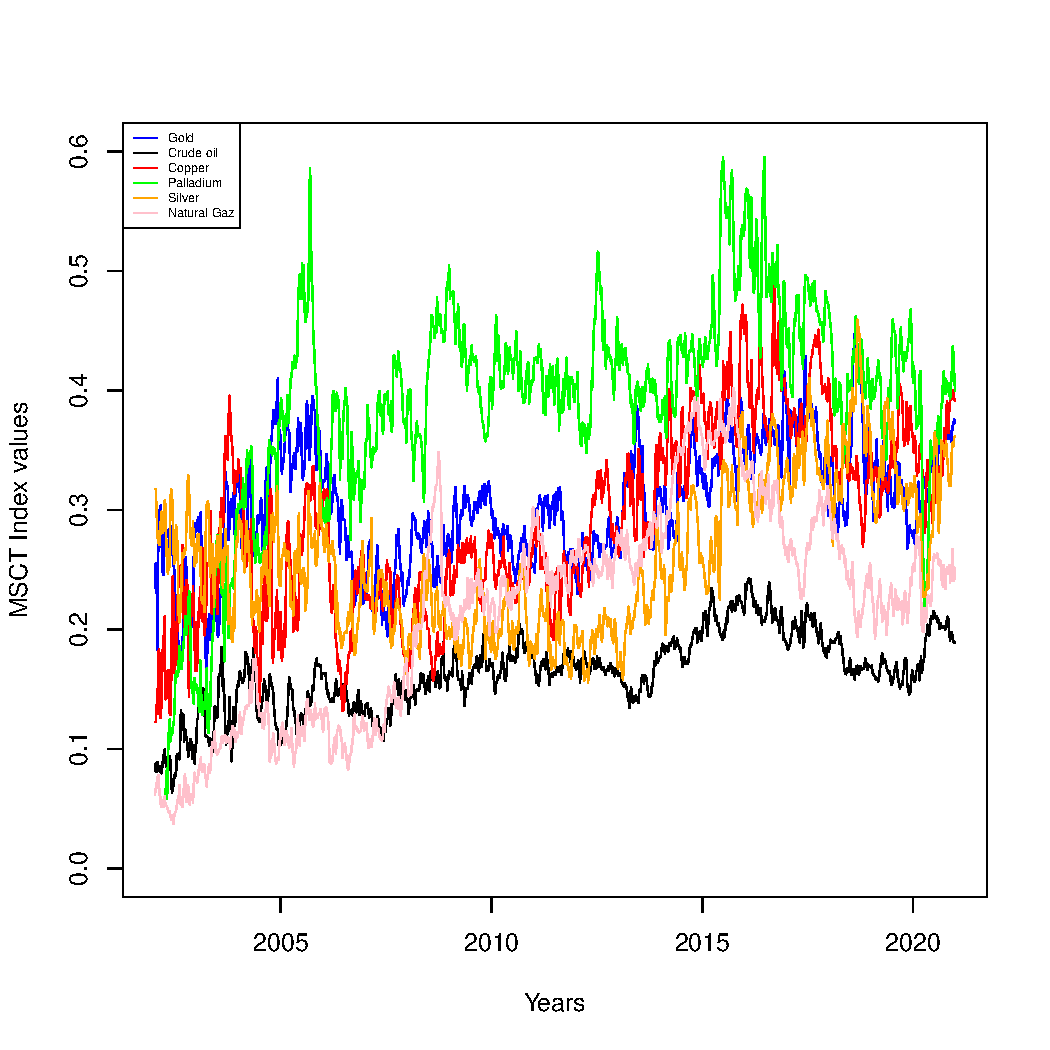
\includegraphics[scale=0.8]{FIG_MSCT}
		\caption{Time series showing the evolution of the Market Share of Non-Commercials (MSCT) index for all commodities in our sample, 4/2007--12/2020. }
		\label{fig:MSCT}
	\end{figure}


	\begin{figure}[h]
	\centering
		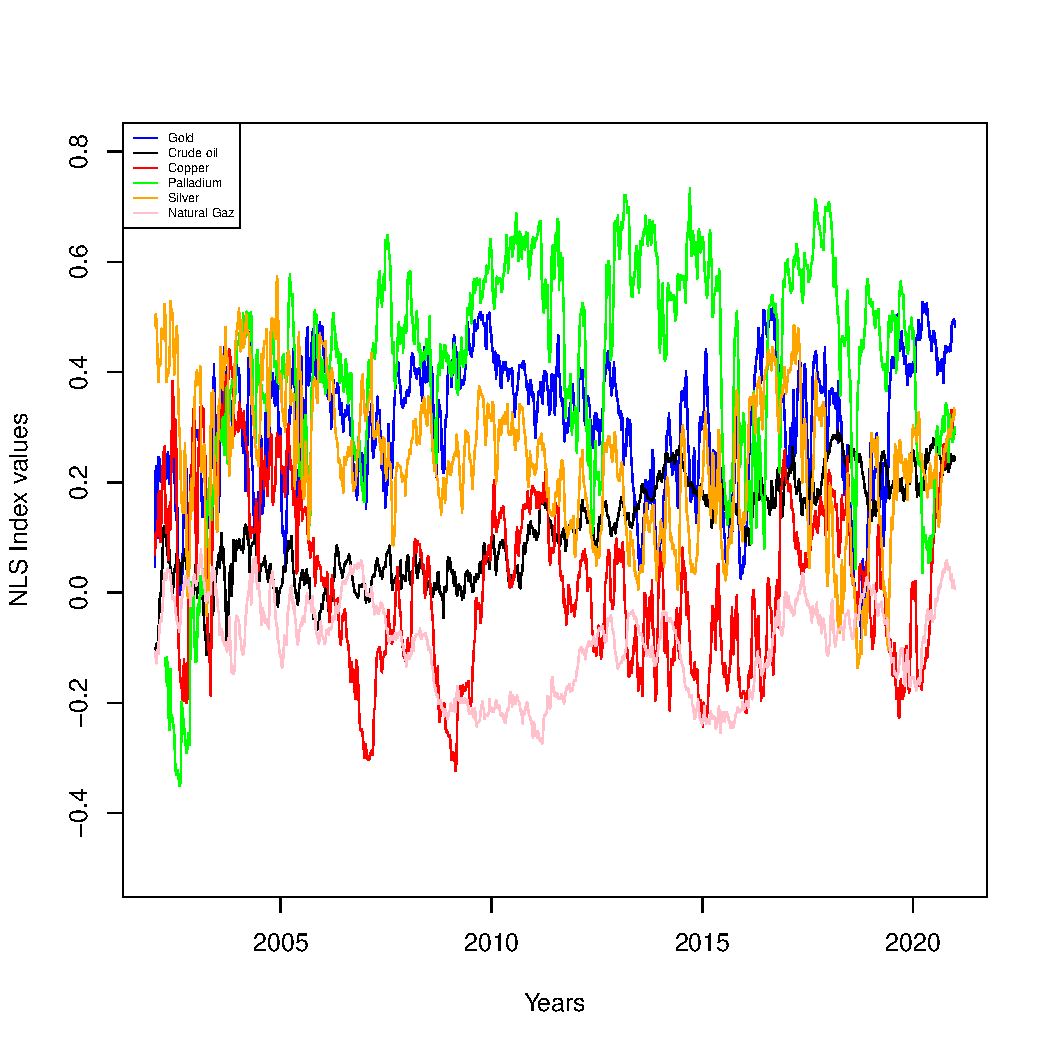
\includegraphics[scale=0.8]{FIG_NLS}
		\caption{Time series showing the evolution of the Net Long Short (NLS) index for all commodities in our sample, 4/2007--12/2020.}
		\label{fig:NLS}
	\end{figure}

	\begin{figure}[h]
	\centering
		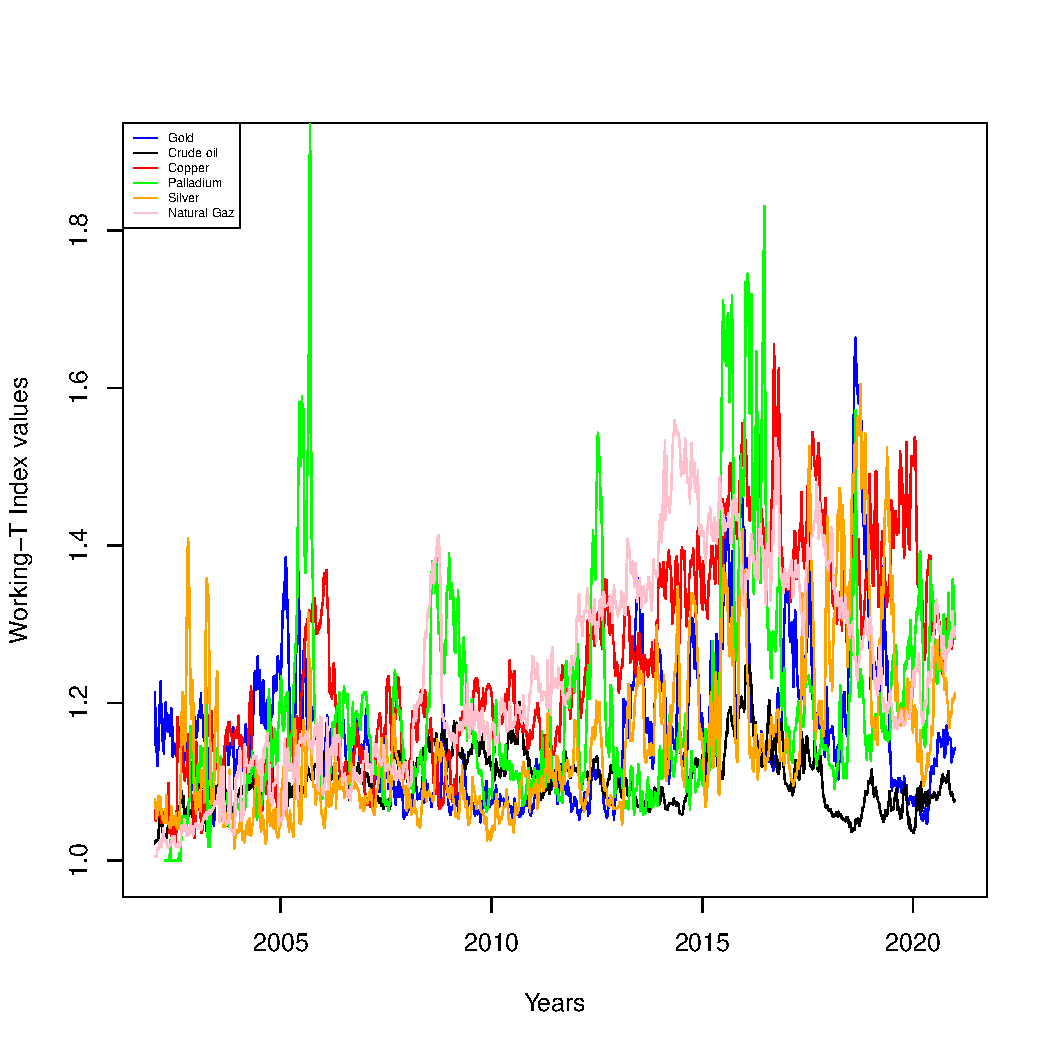
\includegraphics[scale=0.8]{FIG_WT}
		\caption{Time series showing the evolution of the Working's T index for all commodities in our sample, 4/2007--12/2020.}
		\label{fig:WT}
	\end{figure}
	
%% Auteur: Simon-Pierre Boucher, Université Laval, Chapitre 1 : thèse de doctorat

\begin{sidewaystable}
\caption{Announcement (macro \& commodity-specific) and financialization (MSCT) effects on futures returns (Kurov) - Full Sample}
\label{tab:return-fin-full}
\centering
\resizebox{\linewidth}{!}{%
\begin{tabular}{@{}lllllllllllll@{}}
\toprule
\textbf{Commodities}         & \multicolumn{2}{c}{\textbf{Crude Oil}}    & \multicolumn{2}{c}{\textbf{Gold}}          & \multicolumn{2}{c}{\textbf{Copper}}       & \multicolumn{2}{c}{\textbf{Silver}}  & \multicolumn{2}{c}{\textbf{Palladium}}    & \multicolumn{2}{c}{\textbf{Natural Gas}}       \\ \midrule
\textbf{Announcements}       & \multicolumn{1}{c}{$\gamma_m$} & \multicolumn{1}{c}{$\theta_m$} & \multicolumn{1}{c}{$\gamma_m$} & \multicolumn{1}{c}{$\theta_m$} & \multicolumn{1}{c}{$\gamma_m$} & \multicolumn{1}{c}{$\theta_m$} & \multicolumn{1}{c}{$\gamma_m$} & \multicolumn{1}{c}{$\theta_m$} & \multicolumn{1}{c}{$\gamma_m$} & \multicolumn{1}{c}{$\theta_m$} & \multicolumn{1}{c}{$\gamma_m$} & \multicolumn{1}{c}{$\theta_m$} \\ \midrule \multicolumn{13}{c}{\textbf{Macroeconomic News Announcements}} \\ \midrule \textbf{Initial jobless claims}& -0.17269 & 0.81785 & 0.35354*** & -1.16184*** & -0.597*** & 2.60183*** & -0.16447** & 0.52026** & -0.04601 & 0.16735 & 0.05394 & -0.22429 \\ \textbf{ADP Employment}& 0.4279** & -1.75229* & 0.17464 & -0.61362 & 0.99692*** & -3.82781*** & 0.73075*** & -2.26978*** & 0.54531** & -1.51275** & -0.31535 & 1.33729 \\ \textbf{CB Consumer}& 0.07308 & -0.18786 & -0.09105** & 0.38458*** & 0.08368** & -0.44916*** & 0.10301** & -0.30698** & -0.01444 & -0.01458 & 0.02629 & 0.0173 \\ \textbf{Advance retail sales}& 0.05386 & -0.08326 & -0.32683*** & 0.84558*** & -0.16195** & 0.50343** & 0.14357** & -0.42131** & 0.21525** & -0.63829*** & 0.11071 & -0.46188 \\ \textbf{Building permit}& 0.09826* & -0.60141** & 0.04186 & -0.1613 & 0.02706 & -0.18814 & 0.01576 & -0.02451 & 0.02636 & -0.09451 & 0.10885 & -0.37952 \\ \textbf{Construction spending}& 0.20815** & -1.18447** & -0.01436 & 0.01476 & 0.09145** & -0.36507** & -0.00913 & 0.02605 & -0.16893* & 0.41388* & -0.05998 & 0.18388 \\ \textbf{Consumer credit}& -0.07876 & 0.44776 & -0.00196 & -0.00444 & 0.06263** & -0.21898*** & 0.04169 & -0.11137 & -0.02386 & 0.07046 & -0.06683 & 0.26239 \\ \textbf{Consumer price index}& -0.24338*** & 1.22982*** & -0.38533*** & 1.3611*** & 0.32734*** & -1.56094*** & 0.07949* & -0.34742*** & -0.40191*** & 0.81992*** & -0.07215 & 0.26193 \\ \textbf{Durable goods orders}& 0.16941*** & -0.94154** & -0.1604*** & 0.5802*** & 0.20947*** & -0.89069*** & 0.22329*** & -0.64938*** & 0.07477 & -0.12421 & 0.06429 & -0.18845 \\ \textbf{Existing home sales}& 0.0335 & -0.09627 & 0.0082 & -0.04173 & 0.04969 & -0.18234 & 0.10458*** & -0.26099*** & 0.0618 & -0.16229 & 0.15671* & -0.56062* \\ \textbf{Factory orders}& 0.01132 & -0.07277 & 0.0475 & -0.23893* & 0.01524 & -0.17347 & -0.04658 & 0.17274 & 0.00563 & -0.05741 & -0.0032 & 0.08764 \\ \textbf{GDP}& 0.00103 & 0.06139 & -0.05741 & -0.06542 & -0.19739*** & 0.34948** & 0.21569*** & -0.61681*** & -0.09391 & 0.10342 & 0.08718 & -0.31827 \\ \textbf{Housing starts}& -0.05549 & 0.36742 & -0.07544** & 0.14313 & -0.15101*** & 0.35461*** & 0.0625 & -0.16238 & -0.27195*** & 0.59943*** & 0.07248 & -0.31492 \\ \textbf{Industrial production}& -0.05679 & 0.2785 & -0.02818 & 0.00664 & -0.06103 & 0.07782 & 0.03786 & -0.14009 & -0.01019 & -0.00621 & 0.02256 & -0.17454 \\ \textbf{New home sales}& 0.00174 & 0.0692 & -0.00999 & -0.04336 & -0.08205 & 0.12993 & 0.22676*** & -0.59818*** & 0.03259 & -0.07494 & -0.08409 & 0.32422 \\ \textbf{Non-farm employment}& 1.34991*** & -6.24169*** & -0.88205*** & 2.74985*** & 0.71245*** & -2.86793*** & 1.10871*** & -3.4861*** & 1.6227*** & -4.50881*** & -0.53455 & 2.41127 \\ \textbf{Pending home sales}& 0.10027 & -0.47927 & 0.02889 & -0.14231 & 0.04517 & -0.23134 & 0.01093 & 0.00559 & 0.13586 & -0.32594 & 0.0258 & 0.01288 \\ \textbf{Personal consumption}& -0.11005 & 0.60873 & -0.16737*** & 0.5439*** & 0.02927 & -0.10331 & 0.02524 & -0.07862 & 0.0782 & -0.21825 & 0.05713 & -0.33516 \\ \textbf{Personal income}& 0.19418 & -1.11513 & -0.26757* & 0.83348* & 0.08318 & -0.33622 & -0.22522* & 0.70561* & -0.05962 & 0.13436 & 0.1536 & -0.62287 \\ \textbf{Producer price index}& 0.08705 & -0.4889 & -0.07624** & 0.3112*** & 0.06089* & -0.3317** & 0.03516 & -0.12496 & 0.13857** & -0.35739** & -0.03556 & 0.06394 \\ \textbf{Trade balance}& 0.11354* & -0.76201* & 0.0375 & -0.13638 & -0.01022 & 0.05537 & 0.00892 & -0.0516 & -0.07984 & 0.19137 & -0.01249 & 0.10325 \\  \midrule \multicolumn{13}{c}{\textbf{Announcements specific to commodity markets}} \\ \midrule \textbf{Crude Oil Weekly inventory}& -0.02105 & -0.75799*** &  &  &  &  &  &  &  &  &  &  \\ \textbf{Natural Gas Weekly inventory}&  &  &  &  &  &  &  &  &  &  & 0.09661 & -1.73275*** \\  \midrule \textbf{Observations}             &\multicolumn{2}{c}{ 1193455 }                                                 & \multicolumn{2}{c}{ 1190001 }                                                 & \multicolumn{2}{c}{ 1180816 }                                                 & \multicolumn{2}{c}{ 1138696 }                                                 & \multicolumn{2}{c}{ 749168 }                                                   & \multicolumn{2}{c}{ 1101836 }                                                 \\ \textbf{$R^2$}             &\multicolumn{2}{c}{ 0.001836 }                                                 & \multicolumn{2}{c}{ 0.001414 }                                                 & \multicolumn{2}{c}{ 0.001048 }                                                 & \multicolumn{2}{c}{ 0.000379 }                                                 & \multicolumn{2}{c}{ 0.000266 }                                                   & \multicolumn{2}{c}{ 0.001196 }                                                 \\ \bottomrule 
\end{tabular}
}
\begin{tablenotes}\item 
    \singlespacing
    \footnotesize
    This table presents estimates of eq. \ref{eq:Model 1}, $R_{t}^{t+\tau}=\alpha+\sum_{m=1}^{22} \gamma_m S_{m,t}+ \delta X_{t,i} + \sum_{m=1}^{22} \theta_m (S_{m,t} \cdot X_t)+\beta R_{t-\tau}^{t}+\epsilon_{t}$ using the method proposed by \citet{kurov2019price} and financialization variable $MSCT_t$. The $\gamma_m$ coefficients capture the instantaneous change in return when an announcement has just occurred and especially if that announcement was unanticipated. The coefficients $\theta_m$ capture the instantaneous change in return when an announcement has just occurred in conjunction with the level of financialization.
\end{tablenotes}
\end{sidewaystable}

\begin{sidewaystable}
\caption{Announcement (macro \& commodity-specific) and financialization (WT) effects on futures returns (Kurov) - Full Sample}
\label{tab:return-fin-full}
\centering
\resizebox{\linewidth}{!}{%
\begin{tabular}{@{}lllllllllllll@{}}
\toprule
\textbf{Commodities}         & \multicolumn{2}{c}{\textbf{Crude Oil}}    & \multicolumn{2}{c}{\textbf{Gold}}          & \multicolumn{2}{c}{\textbf{Copper}}       & \multicolumn{2}{c}{\textbf{Silver}}  & \multicolumn{2}{c}{\textbf{Palladium}}    & \multicolumn{2}{c}{\textbf{Natural Gas}}       \\ \midrule
\textbf{Announcements}       & \multicolumn{1}{c}{$\gamma_m$} & \multicolumn{1}{c}{$\theta_m$} & \multicolumn{1}{c}{$\gamma_m$} & \multicolumn{1}{c}{$\theta_m$} & \multicolumn{1}{c}{$\gamma_m$} & \multicolumn{1}{c}{$\theta_m$} & \multicolumn{1}{c}{$\gamma_m$} & \multicolumn{1}{c}{$\theta_m$} & \multicolumn{1}{c}{$\gamma_m$} & \multicolumn{1}{c}{$\theta_m$} & \multicolumn{1}{c}{$\gamma_m$} & \multicolumn{1}{c}{$\theta_m$} \\ \midrule \multicolumn{13}{c}{\textbf{Macroeconomic News Announcements}} \\ \midrule \textbf{Initial jobless claims}& -2.72317*** & 2.54402*** & 1.95068*** & -1.85382*** & -2.73165*** & 2.48198*** & -0.51585*** & 0.39918** & 0.41845** & -0.35212** & 0.26294 & -0.21395 \\ \textbf{ADP Employment}& 0.42334 & -0.31925 & -1.87022*** & 1.70565*** & 3.16957*** & -2.80197*** & 1.40773*** & -0.99856*** & -0.34768 & 0.25256 & -0.30605 & 0.23151 \\ \textbf{CB Consumer}& -0.51008 & 0.50063 & -0.11058**& 0.12443***& 0.33198*** & -0.31746*** & 0.248*** & -0.18412*** & 0.09918 & -0.09728 & -0.0141 & 0.03475 \\ \textbf{Advance retail sales}& 2.61014*** & -2.44694*** & 0.1169 & -0.13731 & 0.10808 & -0.10441 & 0.71952*** & -0.54159*** & -0.22639 & 0.15872 & 0.29694 & -0.2362 \\ \textbf{Building permit}& -0.26396 & 0.24817 & 0.04458 & -0.0487 & 0.14859* & -0.14616** & -0.00195 & 0.00648 & -0.04085 & 0.01909 & 0.24231 & -0.17974 \\ \textbf{Construction spending}& 0.51461 & -0.47216 & 0.09324 & -0.08744* & 0.24955** & -0.21877*** & 0.05299 & -0.0402 & -0.20469** & 0.17555** & -0.10808 & 0.07458 \\ \textbf{Consumer credit}& -0.10509 & 0.09496 & 0.01988 & -0.01963 & 0.12335** & -0.10397*** & 0.05805 & -0.04096 & -0.1005 & 0.08898 & -0.09181 & 0.07137 \\ \textbf{Consumer price index}& 0.12419 & -0.14639 & -0.75336*** & 0.69558*** & 1.74249*** & -1.56473*** & 0.42986*** & -0.35482*** & -0.15683* & 0.08383 & -0.33289* & 0.25382* \\ \textbf{Durable goods orders}& 0.66055*** & -0.6145*** & -0.2421*** & 0.22889*** & 0.48551*** & -0.43654*** & 0.35842*** & -0.26175*** & 0.13976* & -0.10394* & 0.24398* & -0.17469 \\ \textbf{Existing home sales}& 0.81342*** & -0.73895*** & 0.02932 & -0.02948 & 0.12157 & -0.10252 & 0.2302*** & -0.15948** & 0.04782 & -0.04563 & 0.2283 & -0.17186 \\ \textbf{Factory orders}& -0.07882 & 0.0723 & 0.043 & -0.06182 & 0.08843 & -0.10148 & -0.11794 & 0.09612 & -0.0023 & -0.01385 & -0.15365 & 0.13642 \\ \textbf{GDP}& -0.29895 & 0.28467 & -0.13702* & 0.18425*** & -0.02867 & -0.06026 & 0.42527*** & -0.31542*** & 0.04028 & -0.07835 & 0.18286 & -0.13845 \\ \textbf{Housing starts}& -0.31531 & 0.29813 & 0.00216 & -0.0239 & -0.0774 & 0.02949 & 0.15035** & -0.10519** & -0.13741* & 0.10154* & 0.12223 & -0.10169 \\ \textbf{Industrial production}& -0.5416 & 0.49076 & -0.09771 & 0.06132 & -0.20799* & 0.14116 & 0.09847 & -0.08164 & 0.0231 & -0.03144 & 0.09067 & -0.08929 \\ \textbf{New home sales}& -0.51511 & 0.48718 & -0.11535* & 0.11647** & -0.14097 & 0.08081 & 0.40194*** & -0.28602*** & 0.10254 & -0.08375 & -0.21011 & 0.16145 \\ \textbf{Non-farm employment}& -0.64716 & 0.64998 & -3.93856*** & 3.59324*** & 2.96334*** & -2.64398*** & 1.79631*** & -1.28066*** & 0.47681 & -0.33898 & -0.4552 & 0.36905 \\ \textbf{Pending home sales}& -0.49865 & 0.46766 & 0.04389 & -0.05302 & 0.10203 & -0.10227 & -0.02135 & 0.02569 & 0.19396 & -0.1596 & 0.10408 & -0.05986 \\ \textbf{Personal consumption}& -0.0791 & 0.07278 & -0.12236** & 0.1171** & 0.01867 & -0.01621 & 0.02184 & -0.01697 & -0.24043** & 0.19378** & 0.00376 & -0.02339 \\ \textbf{Personal income}& 0.11852 & -0.1312 & -0.60773*** & 0.55793*** & 0.75563** & -0.67091** & -0.64049** & 0.46742** & 0.0692 & -0.06482 & 1.14311* & -0.91757* \\ \textbf{Producer price index}& -0.22354 & 0.2074 & -0.19504*** & 0.1896*** & 0.16443* & -0.16207** & 0.16863* & -0.1319* & 0.11889 & -0.10135 & 0.0306 & -0.03836 \\ \textbf{Trade balance}& 0.30554 & -0.27147 & -0.1287** & 0.12051** & 0.05369 & -0.04912 & 0.02587 & -0.02434 & -0.01768 & 0.01505 & -0.06141 & 0.06019 \\  \midrule \multicolumn{13}{c}{\textbf{Announcements specific to commodity markets}} \\ \midrule \textbf{Crude Oil Weekly inventory}& -0.11062 & -0.03484 &  &  &  &  &  &  &  &  &  &  \\ \textbf{Natural Gas Weekly inventory}&  &  &  &  &  &  &  &  &  &  & 0.31404*** & -0.52644*** \\  \midrule \textbf{Observations}             &\multicolumn{2}{c}{ 1193455 }                                                 & \multicolumn{2}{c}{ 1190001 }                                                 & \multicolumn{2}{c}{ 1180816 }                                                 & \multicolumn{2}{c}{ 1138696 }                                                 & \multicolumn{2}{c}{ 749168 }                                                   & \multicolumn{2}{c}{ 1101836 }                                                 \\ \textbf{$R^2$}             &\multicolumn{2}{c}{ 0.001788 }                                                 & \multicolumn{2}{c}{ 0.00183 }                                                 & \multicolumn{2}{c}{ 0.001339 }                                                 & \multicolumn{2}{c}{ 0.000396 }                                                 & \multicolumn{2}{c}{ 0.00022 }                                                   & \multicolumn{2}{c}{ 0.001204 }                                                 \\ \bottomrule 
\end{tabular}
}
\begin{tablenotes}\item 
    \singlespacing
    \footnotesize
    This table presents estimates of eq. \ref{eq:Model 1}, $R_{t}^{t+\tau}=\alpha+\sum_{m=1}^{22} \gamma_m S_{m,t}+ \delta X_{t,i} + \sum_{m=1}^{22} \theta_m (S_{m,t} \cdot X_t)+\beta R_{t-\tau}^{t}+\epsilon_{t}$ using the method proposed by \citet{kurov2019price} and financialization variable $WT_t$. The $\gamma_m$ coefficients capture the instantaneous change in return when an announcement has just occurred and especially if that announcement was unanticipated. The coefficients $\theta_m$ capture the instantaneous change in return when an announcement has just occurred in conjunction with the level of financialization.
\end{tablenotes}
\end{sidewaystable}


\begin{sidewaystable}
\caption{Announcement (macro \& commodity-specific) and financialization (PCA) effects on futures returns (Kurov) - Full Sample}
\label{tab:return-fin-full}
\centering
\resizebox{\linewidth}{!}{%
\begin{tabular}{@{}lllllllllllll@{}}
\toprule
\textbf{Commodities}         & \multicolumn{2}{c}{\textbf{Crude Oil}}    & \multicolumn{2}{c}{\textbf{Gold}}          & \multicolumn{2}{c}{\textbf{Copper}}       & \multicolumn{2}{c}{\textbf{Silver}}  & \multicolumn{2}{c}{\textbf{Palladium}}    & \multicolumn{2}{c}{\textbf{Natural Gas}}       \\ \midrule
\textbf{Announcements}       & \multicolumn{1}{c}{$\gamma_m$} & \multicolumn{1}{c}{$\theta_m$} & \multicolumn{1}{c}{$\gamma_m$} & \multicolumn{1}{c}{$\theta_m$} & \multicolumn{1}{c}{$\gamma_m$} & \multicolumn{1}{c}{$\theta_m$} & \multicolumn{1}{c}{$\gamma_m$} & \multicolumn{1}{c}{$\theta_m$} & \multicolumn{1}{c}{$\gamma_m$} & \multicolumn{1}{c}{$\theta_m$} & \multicolumn{1}{c}{$\gamma_m$} & \multicolumn{1}{c}{$\theta_m$} \\ \midrule \multicolumn{13}{c}{\textbf{Macroeconomic News Announcements}} \\ \midrule \textbf{Initial jobless claims}& -0.03678*** & 0.03459 & 0.17292*** & -2.3094*** & 0.18376*** & -2.01994*** & 0.00293 & -1.36178*** & -1e-05 & -0.07918 & -0.00556 & -0.01098 \\ \textbf{ADP Employment}& 0.14017*** & -0.0595* & -0.07777*** & 0.15403*** & -0.10969*** & 0.22191*** & 0.06766*** & 0.03644** & -0.00127 & 0.00059 & 0.0838 & 0.10394 \\ \textbf{CB Consumer}& 0.04236*** & -0.01208 & -0.03419*** & 0.13402*** & -0.04358*** & -0.25341*** & 0.00643 & -0.1673*** & -0.01969* & -0.01538 & 0.03057** & 0.00144 \\ \textbf{Advance retail sales}& 0.04375*** & -0.0088 & -0.0395*** & 0.01267*** & -0.01565 & -0.02849*** & 0.00998 & -0.01919*** & -0.02026** & -0.01189 & -0.00374 & -0.00494 \\ \textbf{Building permit}& 0.00298 & 0.01757* & -0.01135** & -0.00218 & -0.02413*** & 0.00056 & 0.00728 & -0.03935*** & -0.01645** & -0.01596 & 0.01235 & -0.02035* \\ \textbf{Construction spending}& 0.00809 & -0.03581** & -0.00832 & -0.00536 & -0.00981 & -0.01372** & -0.00062 & -5e-04 & 0.00913 & 0.00036 & -0.01243 & 0.01026 \\ \textbf{Consumer credit}& -0.00322 & 0.01332 & -0.00289 & -0.00601 & 7e-04 & -0.02031*** & 0.00559 & 0.00016 & 0.00679 & 0.02454** & 0.00143 & 0.01181 \\ \textbf{Consumer price index}& 0.03543*** & -0.03692*** & -0.05483*** & -0.00176 & -0.10937*** & -0.01011*** & -0.03288*** & -0.00609 & -0.05374*** & 0.00838 & -0.0047 & 0.01551 \\ \textbf{Durable goods orders}& 0.01368*** & -0.03864*** & -0.02515*** & 0.05928*** & -0.03261*** & -0.13181*** & 0.01623*** & -0.02752*** & 0.01345* & 0.014 & 0.01582 & -0.0087 \\ \textbf{Existing home sales}& 0.02008 & -0.01516 & -0.00522 & -0.02186*** & -0.00013 & -0.04068*** & 0.02136*** & -0.03333*** & -0.00779 & -0.01774* & 0.01211 & -0.02662* \\ \textbf{Factory orders}& -0.00062 & 0.00292 & -0.02925*** & -0.0037 & -0.03248*** & -0.00998 & 0.00852 & -0.01503*** & -0.01913 & -0.00578 & 0.01888 & -0.00238 \\ \textbf{GDP}& 0.01182 & -0.00052 & -0.07755*** & -0.00734 & -0.09985*** & -0.01094 & 0.01673** & 0.00996 & -0.0546*** & -0.00249 & 0.00176 & -0.00805 \\ \textbf{Housing starts}& 0.0065 & 0.00892 & -0.02528*** & 0.01492** & -0.04326*** & -0.00336 & 0.0123* & -0.03623*** & -0.01777** & -0.00571 & -0.00875 & -0.0161 \\ \textbf{Industrial production}& -0.00929 & 0.00483 & -0.02642*** & -0.00286 & -0.0404*** & 0.00425 & -0.00738 & -0.01099* & -0.01467 & 0.02633*** & -0.02329 & -0.00628 \\ \textbf{New home sales}& 0.01563 & -0.00546 & -0.01969*** & 0.00467 & -0.04503*** & -0.00625 & 0.03276*** & 0.0022 & 4e-05 & 0.00181 & 0.00065 & 0.01469 \\ \textbf{Non-farm employment}& 0.25893*** & -0.1586*** & -0.19512*** & 0.01115** & -0.14487*** & 0.00684 & 0.08789*** & -0.03551*** & 0.03755*** & -0.01164 & 0.11722* & 0.11886* \\ \textbf{Pending home sales}& 0.02108* & -0.02003 & -0.01773*** & 0.36735*** & -0.01907* & -0.30985*** & 0.01269* & -0.2521*** & -0.00489 & -0.14344*** & 0.02989 & 0.01237 \\ \textbf{Personal consumption}& -0.00695 & 0.01624 & -0.01415*** & -0.00473 & -0.00024 & -0.0081 & 4e-04 & 0.0019 & -0.00336 & -0.02761* & -0.0303* & -0.01222 \\ \textbf{Personal income}& 0.00392 & -0.03088 & -0.03459*** & 0.01316*** & -0.02589* & -0.00167 & -0.01428* & -0.00442 & -0.00842 & 0.00877 & -0.00307 & -0.01861 \\ \textbf{Producer price index}& 0.00342 & -0.01723 & -0.02587*** & 0.04961***& 0.02779*** & -0.04959* & -0.00437 & 0.05207** & -0.00873 & 0.01626 & -0.0194 & 0.00436 \\ \textbf{Trade balance}& -0.01634* & 0.01997** & -0.01255* & 0.01738***& -0.00187 & -0.01307* & -0.00699 & -0.0099 & -0.00033 & -0.02848*** & 0.01383 & 0.01053 \\  \midrule \multicolumn{13}{c}{\textbf{Announcements specific to commodity markets}} \\ \midrule \textbf{Crude Oil Weekly inventory}& -0.148*** & -0.02413*** &  &  &  &  &  &  &  &  &  &  \\ \textbf{Natural Gas Weekly inventory}&  &  &  &  &  &  &  &  &  &  & -0.00805 & 0.00195 \\  \midrule \textbf{Observations}             &\multicolumn{2}{c}{ 1193455 }                                                 & \multicolumn{2}{c}{ 1190001 }                                                 & \multicolumn{2}{c}{ 1180816 }                                                 & \multicolumn{2}{c}{ 1138696 }                                                 & \multicolumn{2}{c}{ 749168 }                                                   & \multicolumn{2}{c}{ 1101836 }                                                 \\ \textbf{$R^2$}             &\multicolumn{2}{c}{ 0.001845 }                                                 & \multicolumn{2}{c}{ 0.001809 }                                                 & \multicolumn{2}{c}{ 0.001278 }                                                 & \multicolumn{2}{c}{ 0.000449 }                                                 & \multicolumn{2}{c}{ 0.000228 }                                                   & \multicolumn{2}{c}{ 0.000483 }                                                 \\ \bottomrule 
\end{tabular}
}
\begin{tablenotes}\item 
    \singlespacing
    \footnotesize
    This table presents estimates of eq. \ref{eq:Model 1}, $R_{t}^{t+\tau}=\alpha+\sum_{m=1}^{22} \gamma_m S_{m,t}+ \delta X_{t,i} + \sum_{m=1}^{22} \theta_m (S_{m,t} \cdot X_t)+\beta R_{t-\tau}^{t}+\epsilon_{t}$ using the method proposed by \citet{kurov2019price} and financialization variable $PCA_t$. The $\gamma_m$ coefficients capture the instantaneous change in return when an announcement has just occurred and especially if that announcement was unanticipated. The coefficients $\theta_m$ capture the instantaneous change in return when an announcement has just occurred in conjunction with the level of financialization.
\end{tablenotes}
\end{sidewaystable}

\begin{sidewaystable}
\caption{Announcement (macro \& commodity-specific) and financialization (MSCT) effects on futures conditional variance - Full Sample}
\label{tab:return-fin-full}
\centering
\resizebox{\linewidth}{!}{%
\begin{tabular}{@{}lllllllllllll@{}}
\toprule
\textbf{Commodities}         & \multicolumn{2}{c}{\textbf{Crude Oil}}    & \multicolumn{2}{c}{\textbf{Gold}}          & \multicolumn{2}{c}{\textbf{Copper}}       & \multicolumn{2}{c}{\textbf{Silver}}  & \multicolumn{2}{c}{\textbf{Palladium}}    & \multicolumn{2}{c}{\textbf{Natural Gas}}       \\ \midrule
\textbf{Announcements}            & \multicolumn{1}{c}{\textbf{$\Phi_m$}} & \multicolumn{1}{c}{\textbf{$\phi_m$}} & \multicolumn{1}{c}{\textbf{$\Phi_m$}} & \multicolumn{1}{c}{\textbf{$\phi_m$}} & \multicolumn{1}{c}{\textbf{$\Phi_m$}} & \multicolumn{1}{c}{\textbf{$\phi_m$}} & \multicolumn{1}{c}{\textbf{$\Phi_m$}} & \multicolumn{1}{c}{\textbf{$\phi_m$}} & \multicolumn{1}{c}{\textbf{$\Phi_m$}} & \multicolumn{1}{c}{\textbf{$\phi_m$}} & \multicolumn{1}{c}{\textbf{$\Phi_m$}} & \multicolumn{1}{c}{\textbf{$\phi_m$}} \\ \midrule \multicolumn{13}{c}{\textbf{Macroeconomic News Announcements}} \\ \midrule \textbf{Initial jobless claims}& 0.05925* & -0.15137 & 0.10896*** & -0.1668*** & 0.09455*** & -0.05388 & 0.10238*** & -0.23646*** & 0.08883** & -0.0227 & 0.08759*** & -0.35915*** \\ \textbf{ADP Employment}& -0.04522 & 0.23501 & 1e-05 & 0.1115 & 0.00192 & 0.16495 & 0.10563*** & -0.23408*** & -0.18627** & 0.38112* & 0.09939 & -0.33362 \\ \textbf{CB Consumer}& 0.11565 & -0.44436 & 0.037 & -0.00272 & 0.11009*** & -0.20939** & 0.16917*** & -0.4302*** & 0.11164 & -0.19555 & 0.04412 & -0.18347 \\ \textbf{Advance retail sales}& -0.06522 & 0.60081 & 0.10903*** & -0.57308*** & -0.0059 & 0.42894*** & 0.12213*** & -0.28663*** & -0.11342 & 0.40553** & 0.18427*** & -0.58649** \\ \textbf{Building permit}& 0.13647** & -0.6803* & 0.15975*** & -0.40363*** & 0.13257*** & -0.37946*** & 0.09318*** & -0.26484*** & 0.06884 & -0.02091 & 0.09663 & -0.2679 \\ \textbf{Construction spending}& 0.17169** & -0.6718 & 0.06784** & -0.03464 & 0.08161*** & -0.04999 & 0.23574*** & -0.59357*** & 0.06108 & -0.0232 & 0.06011 & -0.14725 \\ \textbf{Consumer credit}& 0.02806 & -0.12063 & 0.00195 & 0.017 & 0.00768 & 0.03847 & 0.03244 & -0.08667 & 0.0302 & -0.05883 & -0.01208 & 0.04883 \\ \textbf{Consumer price index}& 0.505*** & -2.58419*** & 0.22236*** & -1.03864*** & -0.18351*** & 1.25727*** & -0.03708 & 0.42019*** & 0.4052*** & -0.73505*** & 0.15262* & -0.49541 \\ \textbf{Durable goods orders}& 0.05156 & -0.1188 & 0.07628*** & -0.14679* & 0.05991** & -0.0485 & 0.08978*** & -0.25025*** & -0.03253 & 0.21023 & 0.0481 & -0.14869 \\ \textbf{Existing home sales}& 0.09818 & -0.35134 & 0.08388*** & -0.15792* & 0.11222*** & -0.28496*** & 0.14518*** & -0.3764*** & 0.51154*** & -1.1596*** & 0.13083** & -0.35498 \\ \textbf{Factory orders}& -0.09301 & 0.76921* & 6e-05 & 0.14911** & 0.0174 & 0.11481 & 0.1282*** & -0.31586*** & 0.04772 & -0.04955 & -0.01208 & 0.24407 \\ \textbf{GDP}& -0.0099 & 0.17292 & 0.10772*** & -0.13234 & 0.17949*** & -0.33478*** & 0.10718*** & -0.25421*** & 0.15523 & -0.20066 & 0.01826 & -0.11232 \\ \textbf{Housing starts}& 0.11427 & -0.55905 & 0.11941*** & -0.28247*** & 0.09153*** & -0.23646** & 0.09612*** & -0.26577*** & 0.11155 & -0.15951 & 0.06725 & -0.19907 \\ \textbf{Industrial production}& 0.12609* & -0.74582* & 0.11232*** & -0.281*** & 0.05302* & -0.11705 & 0.07437** & -0.21906** & 0.04234 & -0.10858 & 0.10674 & -0.44216* \\ \textbf{New home sales}& 0.01205 & 0.027 & 0.10477*** & -0.1805** & 0.15113*** & -0.31343*** & 0.15373*** & -0.39662*** & -0.01773 & 0.11541 & 0.06611 & -0.23478 \\ \textbf{Non-farm employment}& 0.12564** & 0.33361 & 0.15492*** & 0.30003*** & 0.33147*** & 0.08 & 0.32639*** & -0.61599*** & 0.08488 & 0.17016 & 0.23229*** & -0.62294*** \\ \textbf{Pending home sales}& -0.023 & 0.30789 & 0.06577** & -0.15417* & 0.08007*** & -0.17627* & 0.18716*** & -0.47817*** & 0.1228 & -0.21443 & 0.27636*** & -0.93667*** \\ \textbf{Personal consumption}& -0.00889 & 0.10034 & 0.01476 & 0.06256 & -0.00567 & 0.19038 & 0.10021*** & -0.29489*** & 0.18689** & -0.29472 & 0.11014 & -0.13738 \\ \textbf{Personal income}& 0.0089 & 0.0197 & 0.09365*** & -0.1596* & 0.06349** & -0.02569 & 0.04245 & -0.09077 & 0.16881* & -0.2676 & 0.08754 & -0.12162 \\ \textbf{Producer price index}& 0.03537 & 0.05367 & 0.06354** & -0.05404 & 0.05567* & 0.05309 & 0.06971** & -0.18087* & 0.0547 & 0.10281 & 0.05762 & -0.18468 \\ \textbf{Trade balance}& -0.03747 & 0.55194 & -0.0377 & 0.30357*** & -0.01079 & 0.32545*** & -0.02921 & 0.12079 & -0.13435 & 0.49068** & 0.0182 & -0.04505 \\  \midrule \multicolumn{13}{c}{\textbf{Announcements specific to commodity markets}} \\ \midrule \textbf{Crude Oil Weekly inventory}& -0.12532** & 1.35013*** &  &  &  &  &  &  &  &  &  &  \\ \textbf{Natural Gas Weekly inventory}&  &  &  &  &  &  &  &  &  &  & 0.65248*** & -0.17546 \\  \midrule \textbf{Observations}             &\multicolumn{2}{c}{ 1193455 }                                                 & \multicolumn{2}{c}{ 1190001 }                                                 & \multicolumn{2}{c}{ 1180816 }                                                 & \multicolumn{2}{c}{ 1138696 }                                                 & \multicolumn{2}{c}{ 749168 }                                                   & \multicolumn{2}{c}{ 1101836 }                                                 \\ \textbf{$R^2$}             &\multicolumn{2}{c}{ 0.070041 }                                                 & \multicolumn{2}{c}{ 0.082937 }                                                 & \multicolumn{2}{c}{ 0.085948 }                                                 & \multicolumn{2}{c}{ 0.079205 }                                                 & \multicolumn{2}{c}{ 0.060702 }                                                   & \multicolumn{2}{c}{ 0.137585 }                                                 \\ \bottomrule 
\end{tabular}
}
\begin{tablenotes}\item 
        \singlespacing
        \footnotesize
        This table presents estimates of eq. \ref{eqn:VarianceEqn} using financialization variable $MSCT_t$. The equation is $\sigma_{t}^2=\alpha_0+\alpha_1 \sigma_{t-1}^2+\alpha_2 \epsilon_t^2 +\sum_{m=1}^{22} \Phi_m D_{m,t}+\beta X_{i,t}+\sum_{k=1}^n \phi_k I_{kt} + \sum_{h=1}^{23} \rho_h D_h$ where $I_{kt}=D_{m,t} \cdot X_{i,t}$ and $D_{m,t}$ is a macro announcement dummy variable for release $m$. The $\Phi_m$ coefficients capture the instantaneous change in the conditional variance when an announcement has just occurred. The $\phi_m$ coefficients capture the conditional variance when an announcement has just occurred in conjunction with the level of financialization.
\end{tablenotes}
\end{sidewaystable}


\begin{sidewaystable}
\caption{Announcement (macro \& commodity-specific) and financialization (WT) effects on futures conditional variance - Full Sample}
\label{tab:return-fin-full}
\centering
\resizebox{\linewidth}{!}{%
\begin{tabular}{@{}lllllllllllll@{}}
\toprule
\textbf{Commodities}         & \multicolumn{2}{c}{\textbf{Crude Oil}}    & \multicolumn{2}{c}{\textbf{Gold}}          & \multicolumn{2}{c}{\textbf{Copper}}       & \multicolumn{2}{c}{\textbf{Silver}}  & \multicolumn{2}{c}{\textbf{Palladium}}    & \multicolumn{2}{c}{\textbf{Natural Gas}}       \\ \midrule
\textbf{Announcements}            & \multicolumn{1}{c}{\textbf{$\Phi_m$}} & \multicolumn{1}{c}{\textbf{$\phi_m$}} & \multicolumn{1}{c}{\textbf{$\Phi_m$}} & \multicolumn{1}{c}{\textbf{$\phi_m$}} & \multicolumn{1}{c}{\textbf{$\Phi_m$}} & \multicolumn{1}{c}{\textbf{$\phi_m$}} & \multicolumn{1}{c}{\textbf{$\Phi_m$}} & \multicolumn{1}{c}{\textbf{$\phi_m$}} & \multicolumn{1}{c}{\textbf{$\Phi_m$}} & \multicolumn{1}{c}{\textbf{$\phi_m$}} & \multicolumn{1}{c}{\textbf{$\Phi_m$}} & \multicolumn{1}{c}{\textbf{$\phi_m$}} \\ \midrule \multicolumn{13}{c}{\textbf{Macroeconomic News Announcements}} \\ \midrule \textbf{Initial jobless claims}& 0.68002*** & -0.64614*** & 0.15281*** & -0.08378*** & 0.02652 & 0.04416 & 0.27579*** & -0.19031*** & -0.17239*** & 0.20423*** & 0.27005*** & -0.2139*** \\ \textbf{ADP Employment}& -0.47019 & 0.4223 & -0.01923 & 0.0472 & -0.00903 & 0.04749 & 0.34757*** & -0.24204*** & -0.0207 & -0.00301 & 0.20498 & -0.14969 \\ \textbf{CB Consumer}& -0.37554 & 0.37516 & 0.07012* & -0.02924 & 0.22177*** & -0.14299** & 0.42446*** & -0.30064*** & -0.07754 & 0.08641 & 0.07277 & -0.05972 \\ \textbf{Advance retail sales}& 1.70204*** & -1.5762*** & -0.05751 & 0.11507*** & -0.09332 & 0.17281*** & 0.37105*** & -0.26007*** & 0.02908 & 0.0227 & 0.3623** & -0.25696** \\ \textbf{Building permit}& 0.61283** & -0.57485** & 0.16763*** & -0.11916*** & 0.15161** & -0.10565* & 0.26454*** & -0.19526*** & -0.07725 & 0.11015 & 0.36884** & -0.26393** \\ \textbf{Construction spending}& 0.64259** & -0.63159** & 0.01139 & 0.03805 & 0.06963 & -0.00237 & 0.56592*** & -0.39937*** & 0.04072 & 0.00722 & 0.31258** & -0.22487* \\ \textbf{Consumer credit}& 0.48878* & -0.44884* & 0.01283 & -0.00477 & 0.03158 & -0.01134 & 0.1183* & -0.08681 & 0.01177 & -0.00621 & -0.00323 & 0.00332 \\ \textbf{Consumer price index}& 1.10977*** & -0.94981*** & -0.32847*** & 0.37753*** & -0.89008*** & 0.88131*** & -0.01885 & 0.08901 & -0.03522 & 0.10183 & 0.31497* & -0.2268 \\ \textbf{Durable goods orders}& 0.68382** & -0.64996** & 0.12086*** & -0.07851** & 0.11583 & -0.05799 & 0.25023*** & -0.18356*** & -0.08785 & 0.11699 & 0.16045 & -0.11669 \\ \textbf{Existing home sales}& 0.05573 & -0.01683 & 0.15381*** & -0.10313*** & 0.21457*** & -0.15195** & 0.41051*** & -0.29408*** & -0.0158 & 0.0342 & 0.36337** & -0.25174** \\ \textbf{Factory orders}& 0.22588* & -0.24242** & 0.06979** & -0.01869 & 0.07049 & -0.01823 & 0.1448*** & -0.09104** & -0.11259 & 0.11407* & 0.08856 & -0.02839 \\ \textbf{GDP}& 1.04776*** & -0.96689*** & 0.22276*** & -0.13497*** & 0.3015*** & -0.18094** & 0.29061*** & -0.20286*** & -0.17911* & 0.20479** & 0.25799* & -0.20698* \\ \textbf{Housing starts}& 0.75767** & -0.70342*** & 0.13556*** & -0.09225** & 0.07908 & -0.04521 & 0.25881*** & -0.18938*** & -0.01553 & 0.04758 & 0.27817* & -0.20299* \\ \textbf{Industrial production}& 0.6402** & -0.5778** & 0.11675*** & -0.0815** & 0.0834 & -0.05286 & 0.21529*** & -0.16092*** & -0.21996** & 0.17451** & 0.38129** & -0.30157*** \\ \textbf{New home sales}& 0.97426*** & -0.89951*** & 0.14685*** & -0.08583** & 0.2724*** & -0.17463*** & 0.39026*** & -0.27766*** & -0.30446*** & 0.2725*** & 0.22217 & -0.16814 \\ \textbf{Non-farm employment}& -0.0937 & 0.25642*** & 0.16498*** & 0.07474*** & 0.25466*** & 0.08385** & 0.30235*** & -0.13515*** & 0.04956 & 0.08889* & 0.17232*** & -0.08142 \\ \textbf{Pending home sales}& 1.18892*** & -1.10572*** & 0.07322* & -0.04953 & 0.167** & -0.11468* & 0.45683*** & -0.32407*** & -0.14452 & 0.14257* & 0.78572*** & -0.58446*** \\ \textbf{Personal consumption}& -0.31507 & 0.29275 & -0.05932 & 0.08078* & -0.21679** & 0.22255*** & 0.2456*** & -0.18434*** & -0.07594 & 0.11476 & 0.44399*** & -0.28606** \\ \textbf{Personal income}& -0.19473 & 0.18786 & -0.00613 & 0.04084 & -0.12053 & 0.14892** & 0.09199 & -0.06033 & -0.16891 & 0.18424** & 0.45814*** & -0.31138** \\ \textbf{Producer price index}& 0.78935** & -0.75476*** & 0.159*** & -0.0966** & 0.05385 & 0.01382 & 0.1851** & -0.13223** & -0.09369 & 0.15482* & 0.05409 & -0.0349 \\ \textbf{Trade balance}& 0.03272 & 0.0232 & 0.12294*** & -0.05258* & 0.15128*** & -0.0599 & -0.03514 & 0.03411 & -0.40529*** & 0.38817*** & 0.06636 & -0.04655 \\  \midrule \multicolumn{13}{c}{\textbf{Announcements specific to commodity markets}} \\ \midrule \textbf{Crude Oil Weekly inventory}& -0.70751*** & 0.74816*** &  &  &  &  &  &  &  &  &  &  \\ \textbf{Natural Gas Weekly inventory}&  &  &  &  &  &  &  &  &  &  & 0.40076*** & 0.15626*** \\  \midrule \textbf{Observations}             &\multicolumn{2}{c}{ 1193455 }                                                 & \multicolumn{2}{c}{ 1190001 }                                                 & \multicolumn{2}{c}{ 1180816 }                                                 & \multicolumn{2}{c}{ 1138696 }                                                 & \multicolumn{2}{c}{ 749168 }                                                   & \multicolumn{2}{c}{ 1101836 }                                                 \\ \textbf{$R^2$}             &\multicolumn{2}{c}{ 0.069734 }                                                 & \multicolumn{2}{c}{ 0.08076 }                                                 & \multicolumn{2}{c}{ 0.077465 }                                                 & \multicolumn{2}{c}{ 0.074334 }                                                 & \multicolumn{2}{c}{ 0.058964 }                                                   & \multicolumn{2}{c}{ 0.139725 }                                                 \\ \bottomrule 
\end{tabular}
}
\begin{tablenotes}\item 
        \singlespacing
        \footnotesize
        This table presents estimates of eq. \ref{eqn:VarianceEqn} using financialization variable $WT_t$. The equation is $\sigma_{t}^2=\alpha_0+\alpha_1 \sigma_{t-1}^2+\alpha_2 \epsilon_t^2 +\sum_{m=1}^{22} \Phi_m D_{m,t}+\beta X_{i,t}+\sum_{k=1}^n \phi_k I_{kt} + \sum_{h=1}^{23} \rho_h D_h$ where $I_{kt}=D_{m,t} \cdot X_{i,t}$ and $D_{m,t}$ is a macro announcement dummy variable for release $m$. The $\Phi_m$ coefficients capture the instantaneous change in the conditional variance when an announcement has just occurred. The $\phi_m$ coefficients capture the conditional variance when an announcement has just occurred in conjunction with the level of financialization.
\end{tablenotes}
\end{sidewaystable}

\begin{sidewaystable}
\caption{Announcement (macro \& commodity-specific) and financialization (PCA) effects on futures conditional variance - Full Sample}
\label{tab:return-fin-full}
\centering
\resizebox{\linewidth}{!}{%
\begin{tabular}{@{}lllllllllllll@{}}
\toprule
\textbf{Commodities}         & \multicolumn{2}{c}{\textbf{Crude Oil}}    & \multicolumn{2}{c}{\textbf{Gold}}          & \multicolumn{2}{c}{\textbf{Copper}}       & \multicolumn{2}{c}{\textbf{Silver}}  & \multicolumn{2}{c}{\textbf{Palladium}}    & \multicolumn{2}{c}{\textbf{Natural Gas}}       \\ \midrule
\textbf{Announcements}            & \multicolumn{1}{c}{\textbf{$\Phi_m$}} & \multicolumn{1}{c}{\textbf{$\phi_m$}} & \multicolumn{1}{c}{\textbf{$\Phi_m$}} & \multicolumn{1}{c}{\textbf{$\phi_m$}} & \multicolumn{1}{c}{\textbf{$\Phi_m$}} & \multicolumn{1}{c}{\textbf{$\phi_m$}} & \multicolumn{1}{c}{\textbf{$\Phi_m$}} & \multicolumn{1}{c}{\textbf{$\phi_m$}} & \multicolumn{1}{c}{\textbf{$\Phi_m$}} & \multicolumn{1}{c}{\textbf{$\phi_m$}} & \multicolumn{1}{c}{\textbf{$\Phi_m$}} & \multicolumn{1}{c}{\textbf{$\phi_m$}} \\ \midrule \multicolumn{13}{c}{\textbf{Macroeconomic News Announcements}} \\ \midrule \textbf{Initial jobless claims}& 0.03437*** & -0.00823 & 0.0552*** & -0.00654*** & 0.07888*** & 0.0059** & 0.0269*** & -0.01603*** & 0.0773*** & 0.02253*** & -0.00529 & -0.01618*** \\ \textbf{ADP Employment}& -0.00477 & 0.00458 & 0.03562*** & 0.00624** & 0.04721*** & 0.00693 & 0.03104*** & -0.01849*** & -0.02553** & 0.00988 & 0.01291 & -0.01455 \\ \textbf{CB Consumer}& 0.04128*** & -0.01778 & 0.03604*** & -0.00128 & 0.05207*** & -0.01068* & 0.03156*** & -0.02712*** & 0.02804*** & 0.00982 & -0.0037 & -0.00626 \\ \textbf{Advance retail sales}& 0.03765*** & 0.01023 & 0.0758*** & 0.01642*** & 0.11174*** & 0.01853*** & 0.03072*** & -0.02021*** & 0.05521*** & 0.02424** & 0.03283*** & -0.02836*** \\ \textbf{Building permit}& 0.02144** & -0.02233* & 0.029*** & -0.01037*** & 0.02609*** & -0.0075 & 0.00892 & -0.01717*** & 0.05739*** & 0.01372 & 0.02775*** & -0.01562 \\ \textbf{Construction spending}& 0.05934*** & -0.0268** & 0.05567*** & 0.00463 & 0.06674*** & 0.00187 & 0.04501*** & -0.0362*** & 0.04983*** & 0.00036 & 0.02164* & -0.00452 \\ \textbf{Consumer credit}& 0.00807 & -0.00504 & 0.0073* & 0.00036 & 0.01799** & 0.00085 & 0.0049 & -0.00703 & 0.00445 & -0.00307 & 0.00077 & 0.00164 \\ \textbf{Consumer price index}& 0.06615*** & -0.07188*** & 0.11143*** & 0.03583*** & 0.15711*** & 0.0776*** & 0.09737*** & 0.01921*** & 0.09002*** & 0.00887 & 0.02472* & -0.02282 \\ \textbf{Durable goods orders}& 0.03227*** & -0.00746 & 0.02929*** & -0.00587* & 0.04692*** & -0.00369 & 0.01002* & -0.01642*** & 0.05537*** & 0.01923* & 0.00906 & -0.00243 \\ \textbf{Existing home sales}& 0.03883*** & -0.01052 & 0.03349*** & -0.00791** & 0.03398*** & -0.0116** & 0.02534*** & -0.02499*** & 0.02676*** & -0.0231** & 0.03906*** & -0.01568 \\ \textbf{Factory orders}& 0.03896*** & 0.01378 & 0.04819*** & -0.00166 & 0.049*** & -0.00167 & 0.02633*** & -0.01345*** & 0.02636** & 0.00967 & 0.05118*** & 0.01343 \\ \textbf{GDP}& 0.02088* & -0.00101 & 0.06535*** & -0.00903** & 0.08673*** & -0.01293** & 0.02565*** & -0.01752*** & 0.06974*** & 0.02212* & -0.01102 & -0.0037 \\ \textbf{Housing starts}& 0.02013* & -0.02 & 0.02812*** & -0.00765** & 0.02527*** & -0.00191 & 0.01119* & -0.01676*** & 0.04328*** & 0.00276 & 0.01637 & -0.0132 \\ \textbf{Industrial production}& 0.00039 & -0.02707** & 0.02192*** & -0.00784** & 0.02073*** & -0.00423 & 0.00464 & -0.01413*** & -0.00553 & 0.01398 & -0.00774 & -0.01803* \\ \textbf{New home sales}& 0.01775* & -0.00382 & 0.04679*** & -0.00666** & 0.06506*** & -0.01446*** & 0.02708*** & -0.02534*** & 0.02931*** & 0.03269*** & 0.00492 & -0.0074 \\ \textbf{Non-farm employment}& 0.18348*** & 0.00754 & 0.25161*** & 0.00918*** & 0.35358*** & 0.00997** & 0.12672*** & -0.02233*** & 0.15749*** & 0.01124* & 0.06909*** & -0.01272** \\ \textbf{Pending home sales}& 0.02983*** & 0.00692 & 0.01562*** & -0.00387 & 0.03093*** & -0.00866 & 0.03397*** & -0.03016*** & 0.03012*** & 0.01139 & 0.03304*** & -0.03919*** \\ \textbf{Personal consumption}& 0.00782 & 0.00636 & 0.03474*** & 0.0066 & 0.04712*** & 0.02018*** & 0.00518 & -0.01792*** & 0.064*** & 0.01381 & 0.07445*** & -0.00539 \\ \textbf{Personal income}& 0.01186 & 0.00395 & 0.04151*** & 0.00312 & 0.05608*** & 0.01411** & 0.01327** & -0.00574 & 0.05648*** & 0.01527 & 0.05566*** & -0.00347 \\ \textbf{Producer price index}& 0.04478*** & 6e-05 & 0.04641*** & -0.00684** & 0.07015*** & 0.00472 & 0.01203** & -0.01164** & 0.09595*** & 0.01818* & 0.00957 & -0.00571 \\ \textbf{Trade balance}& 0.05754*** & 0.00611 & 0.06174*** & -0.00208 & 0.08048*** & -0.00478 & 0.0095* & 0.00518 & 0.06834*** & 0.04858*** & 0.00677 & -0.00458 \\  \midrule \multicolumn{13}{c}{\textbf{Announcements specific to commodity markets}} \\ \midrule \textbf{Crude Oil Weekly inventory}& 0.10054*** & 0.04502*** &  &  &  &  &  &  &  &  &  &  \\ \textbf{Natural Gas Weekly inventory}&  &  &  &  &  &  &  &  &  &  & 0.60201*** & 0.01299*** \\  \midrule \textbf{Observations}             &\multicolumn{2}{c}{ 1193455 }                                                 & \multicolumn{2}{c}{ 1190001 }                                                 & \multicolumn{2}{c}{ 1180816 }                                                 & \multicolumn{2}{c}{ 1138696 }                                                 & \multicolumn{2}{c}{ 749168 }                                                   & \multicolumn{2}{c}{ 1101836 }                                                 \\ \textbf{$R^2$}             &\multicolumn{2}{c}{ 0.069413 }                                                 & \multicolumn{2}{c}{ 0.083473 }                                                 & \multicolumn{2}{c}{ 0.080587 }                                                 & \multicolumn{2}{c}{ 0.077022 }                                                 & \multicolumn{2}{c}{ 0.057595 }                                                   & \multicolumn{2}{c}{ 0.138209 }                                                 \\ \bottomrule 
\end{tabular}
}
\begin{tablenotes}\item 
        \singlespacing
        \footnotesize
        This table presents estimates of eq. \ref{eqn:VarianceEqn} using financialization variable $PCA_t$. The equation is $\sigma_{t}^2=\alpha_0+\alpha_1 \sigma_{t-1}^2+\alpha_2 \epsilon_t^2 +\sum_{m=1}^{22} \Phi_m D_{m,t}+\beta X_{i,t}+\sum_{k=1}^n \phi_k I_{kt} + \sum_{h=1}^{23} \rho_h D_h$ where $I_{kt}=D_{m,t} \cdot X_{i,t}$ and $D_{m,t}$ is a macro announcement dummy variable for release $m$. The $\Phi_m$ coefficients capture the instantaneous change in the conditional variance when an announcement has just occurred. The $\phi_m$ coefficients capture the conditional variance when an announcement has just occurred in conjunction with the level of financialization.
\end{tablenotes}
\end{sidewaystable}


\begin{sidewaystable}
\caption{Announcement (macro \& commodity-specific) and financialization (NLS) effects on futures returns (Anderson) - Full Sample}
\label{tab:return-fin-full}
\centering
\resizebox{\linewidth}{!}{%
\begin{tabular}{@{}lllllllllllll@{}}
\toprule
\textbf{Commodities}         & \multicolumn{2}{c}{\textbf{Crude Oil}}    & \multicolumn{2}{c}{\textbf{Gold}}          & \multicolumn{2}{c}{\textbf{Copper}}       & \multicolumn{2}{c}{\textbf{Silver}}  & \multicolumn{2}{c}{\textbf{Palladium}}    & \multicolumn{2}{c}{\textbf{Natural Gas}}       \\ \midrule
\textbf{Announcements}       & \multicolumn{1}{c}{$\gamma_m$} & \multicolumn{1}{c}{$\theta_m$} & \multicolumn{1}{c}{$\gamma_m$} & \multicolumn{1}{c}{$\theta_m$} & \multicolumn{1}{c}{$\gamma_m$} & \multicolumn{1}{c}{$\theta_m$} & \multicolumn{1}{c}{$\gamma_m$} & \multicolumn{1}{c}{$\theta_m$} & \multicolumn{1}{c}{$\gamma_m$} & \multicolumn{1}{c}{$\theta_m$} & \multicolumn{1}{c}{$\gamma_m$} & \multicolumn{1}{c}{$\theta_m$} \\ \midrule \multicolumn{13}{c}{\textbf{Macroeconomic News Announcements}} \\ \midrule \textbf{Initial jobless claims}& -0.20891*** & 0.9061*** & 0.50731*** & -0.97114*** & 0.51063*** & -2.13981*** & 0.00021 & 0.07507 & 0.01039 & -0.032 & -0.00357 & -0.19485 \\ \textbf{ADP Employment}& 0.45173** & -1.46738* & -1.14222*** & 2.43057*** & -0.72094*** & 2.70248*** & 0.02497*** & 0.03865 & 0.00844 & -0.14542 & -0.07585* & -1.51614 \\ \textbf{CB Consumer}& 0.14484*** & -0.63881** & -0.08878*** & 0.16713*** & -0.10388*** & 0.29044** & 0.01533 & -0.05446 & -0.06249** & 0.1521** & 0.04502 & 0.01895 \\ \textbf{Advance retail sales}& 0.34355*** & -1.28088*** & -0.15814*** & 0.27864** & -0.10648 & 0.33985 & 0.01673*** & -0.17414** & -0.01786 & 0.12854 & -0.03098 & -0.31058 \\ \textbf{Building permit}& 0.00073 & 0.06874 & -0.04885** & 0.07564 & -0.08094*** & 0.2715** & 0.00333 & 0.04785 & -0.0267 & -0.01651 & 0.08406* & 0.44162 \\ \textbf{Construction spending}& 0.00543 & -0.27533 & -0.00355 & -0.04469 & -0.0406 & 0.10324 & -2e-05 & -0.2557*** & -0.02053 & 0.03996 & -0.02258 & -0.29357 \\ \textbf{Consumer credit}& 0.04711** & -0.24929** & 0.00315 & -0.00784 & -0.01675 & 0.08063 & 0.00687 & -0.00737 & 0.00862 & 0.00177 & -0.00368 & -0.01041 \\ \textbf{Consumer price index}& 0.15051***& -0.38807*& -0.23136*** & 0.50444*** & -0.34769*** & 1.08871*** & -0.04819*** & -0.2652*** & -0.14212*** & 0.33265*** & 0.01172 & 0.2972 \\ \textbf{Durable goods orders}& 0.15807*** & -0.85995*** & -0.09324*** & 0.21884*** & -0.12537*** & 0.48489*** & 0.01974* & -0.03208 & -0.03134 & 0.10911 & -0.00619 & -0.15486 \\ \textbf{Existing home sales}& 0.0952*** & -0.5194** & -0.02447 & 0.07352 & 0.01577 & 0.04042 & 0.03956*** & -0.18063** & 0.00982 & -0.01239 & 0.08939* & 0.43429 \\ \textbf{Factory orders}& 0.08365***& -0.64996***& -0.10092*** & 0.17834** & -0.07923** & 0.21294 & -0.00098 & 0.12717* & -0.02042 & -0.00144 & 0.15062*** & 1.0821*** \\ \textbf{GDP}& 0.05753 & -0.28002 & -0.20942*** & 0.42841*** & -0.21569*** & 0.64717*** & 0.02138* & -0.03772 & -0.06098*** & 0.04409 & -0.03729 & -0.34389 \\ \textbf{Housing starts}& 0.04015 & -0.2285 & -0.09896*** & 0.18737*** & -0.092*** & 0.21459 & 0.00985 & 0.04459 & -5e-04 & -0.02748 & 0.02681 & 0.449 \\ \textbf{Industrial production}& 0.0209 & -0.25746 & -0.01598 & -0.04692 & -0.00092 & -0.22265 & -0.00598 & -0.07704 & -0.02874 & 0.03408 & -0.02236 & -0.11466 \\ \textbf{New home sales}& 0.16685*** & -0.83721*** & -0.06506*** & 0.08061 & -0.03309 & -0.05022 & 0.04081*** & -0.13435* & 0.0218 & -0.06187 & -0.02786 & -0.06245 \\ \textbf{Non-farm employment}& 1.35726*** & -4.93248*** & -3.19871*** & 6.64971*** & -1.02677*** & 4.36787*** & 0.02693*** & 0.89542*** & -0.01806 & 0.52681 & -0.28623*** & -8.25547*** \\ \textbf{Pending home sales}& 0.04473 & -0.07683 & -0.03501 & 0.0416 & -0.02613 & 0.02513 & 0.01395 & -0.22954** & -0.04356* & 0.04623 & -0.03032 & -0.63082** \\ \textbf{Personal consumption}& -0.03606 & 0.0904 & -0.08001*** & 0.15362** & -0.01358 & 0.02453 & 0.00472 & 0.20674* & -0.01678 & 0.04889 & 0.0011 & 0.48395 \\ \textbf{Personal income}& -0.01867 & -0.04312 & -0.1523 & 0.32489 & -0.41786** & 1.73529** & -0.02497* & -0.39453* & -0.01398 & -0.01605 & -0.04883 & -1.39969 \\ \textbf{Producer price index}& 0.11721*** & -0.63144*** & -0.08903*** & 0.18925*** & 0.03121 & -0.21058 & 0.00955 & -0.04159 & -0.08073** & 0.14271** & -0.03766 & -0.19559 \\ \textbf{Trade balance}& 0.00912 & -0.23206 & -0.08945** & 0.23531** & -0.0647 & 0.26249 & -0.00284 & -0.1553 & -0.00057 & 0.04221 & -0.02635 & -0.17741 \\  \midrule \multicolumn{13}{c}{\textbf{Announcements specific to commodity markets}} \\ \midrule \textbf{Crude Oil Weekly inventory}& -0.11351*** & -0.356*** &  &  &  &  &  &  &  &  &  &  \\ \textbf{Natural Gas Weekly inventory}&  &  &  &  &  &  &  &  &  &  & -0.02081*** & -0.29209*** \\  \midrule \textbf{Observations}             &\multicolumn{2}{c}{ 1193455 }                                                 & \multicolumn{2}{c}{ 1190001 }                                                 & \multicolumn{2}{c}{ 1180816 }                                                 & \multicolumn{2}{c}{ 1138696 }                                                 & \multicolumn{2}{c}{ 749168 }                                                   & \multicolumn{2}{c}{ 1101836 }                                                 \\ \textbf{$R^2$}             &\multicolumn{2}{c}{ 0.063036 }                                                 & \multicolumn{2}{c}{ 0.003063 }                                                 & \multicolumn{2}{c}{ 0.000705 }                                                 & \multicolumn{2}{c}{ 0.000328 }                                                 & \multicolumn{2}{c}{ 0.000133 }                                                   & \multicolumn{2}{c}{ 0.001932 }                                                 \\ \bottomrule 
\end{tabular}
}
\begin{tablenotes}\item 
    \singlespacing
    \footnotesize
    This table presents estimates of eq. \ref{eq:Model 1}, $R_{t}^{t+\tau}=\alpha+\sum_{m=1}^{22} \gamma_m S_{m,t}+ \delta X_{t,i} + \sum_{m=1}^{22} \theta_m (S_{m,t} \cdot X_t)+\beta R_{t-\tau}^{t}+\epsilon_{t}$ using the method proposed by \citet{andersen2007real} and financialization variable $NLS_t$. The $\gamma_m$ coefficients capture the instantaneous change in return when an announcement has just occurred and especially if that announcement was unanticipated. The coefficients $\theta_m$ capture the instantaneous change in return when an announcement has just occurred in conjunction with the level of financialization.
\end{tablenotes}
\end{sidewaystable}

\begin{sidewaystable}
\caption{Announcement (macro \& commodity-specific) and financialization (MSCT) effects on futures returns (Anderson) - Full Sample}
\label{tab:return-fin-full}
\centering
\resizebox{\linewidth}{!}{%
\begin{tabular}{@{}lllllllllllll@{}}
\toprule
\textbf{Commodities}         & \multicolumn{2}{c}{\textbf{Crude Oil}}    & \multicolumn{2}{c}{\textbf{Gold}}          & \multicolumn{2}{c}{\textbf{Copper}}       & \multicolumn{2}{c}{\textbf{Silver}}  & \multicolumn{2}{c}{\textbf{Palladium}}    & \multicolumn{2}{c}{\textbf{Natural Gas}}       \\ \midrule
\textbf{Announcements}       & \multicolumn{1}{c}{$\gamma_m$} & \multicolumn{1}{c}{$\theta_m$} & \multicolumn{1}{c}{$\gamma_m$} & \multicolumn{1}{c}{$\theta_m$} & \multicolumn{1}{c}{$\gamma_m$} & \multicolumn{1}{c}{$\theta_m$} & \multicolumn{1}{c}{$\gamma_m$} & \multicolumn{1}{c}{$\theta_m$} & \multicolumn{1}{c}{$\gamma_m$} & \multicolumn{1}{c}{$\theta_m$} & \multicolumn{1}{c}{$\gamma_m$} & \multicolumn{1}{c}{$\theta_m$} \\ \midrule \multicolumn{13}{c}{\textbf{Macroeconomic News Announcements}} \\ \midrule \textbf{Initial jobless claims}& -0.67794*** & 3.12017*** & 0.03195 & 0.04917 & -0.20177** & 1.24934*** & -1.01824*** & 3.21269*** & -0.01397 & 0.02323 & 0.1097 & -0.43299 \\ \textbf{ADP Employment}& 0.50903 & -2.14381 & -0.4162 & 0.99778 & 0.64175** & -2.73129*** & 0.45531 & -1.38772 & 0.69 & -1.9272 & -0.47827 & 2.06259 \\ \textbf{CB Consumer}& 0.20013 & -0.84023 & 0.06419 & -0.2893** & 0.08507 & -0.48313** & 0.13493*** & -0.37092** & 0.01429 & -0.05217 & 0.02897 & 0.05342 \\ \textbf{Advance retail sales}& 0.14572 & -0.45335 & -0.25083*** & 0.64552** & -0.15033 & 0.42034 & 0.4699*** & -1.3663*** & 0.24274 & -0.69388 & 0.28765 & -1.2416 \\ \textbf{Building permit}& -0.10029 & 0.65151 & 0.04623 & -0.20712 & 0.0149 & -0.16046 & 0.00601 & -0.00704 & -0.04607 & 0.0378 & 0.12356 & -0.34344 \\ \textbf{Construction spending}& 0.16648 & -1.15194** & 0.04867* & -0.21332*** & 0.08287 & -0.39379* & 0.00917 & -0.03016 & -0.09164 & 0.20709 & 0.07985 & -0.25978 \\ \textbf{Consumer credit}& -0.05195 & 0.33235 & 0.04145 & -0.12255 & 0.07716** & -0.26229** & 0.07125*** & -0.19207** & -0.00352 & 0.02594 & -0.03806 & 0.13967 \\ \textbf{Consumer price index}& 0.60061***& -3.01995***& -0.46468***& 1.63686***& 0.36514*** & -1.90912*** & -0.27955*** & 0.77607*** & -0.56038*** & 1.15892*** & -0.12099 & 0.36218 \\ \textbf{Durable goods orders}& 0.30429** & -1.62314** & -0.20179***& 0.69858***& 0.20995*** & -0.9062*** & 0.21842*** & -0.61854*** & -0.14049 & 0.3662 & 0.10203 & -0.28336 \\ \textbf{Existing home sales}& 0.14684 & -0.58592 & 0.0955* & -0.3012* & 0.09509** & -0.2746 & 0.15792*** & -0.40824*** & 0.16495 & -0.37892 & 0.12119 & -0.42035 \\ \textbf{Factory orders}& 0.13238 & -1.19791** & 0.04561 & -0.26187* & -0.01704 & -0.05765 & -0.13725*** & 0.44763*** & 0.06013 & -0.1888 & -0.13539 & 0.48312 \\ \textbf{GDP}& 0.00368 & 0.06479 & -0.00351 & -0.13506 & -0.10752 & 0.14444 & 0.27624*** & -0.83459*** & -0.29761** & 0.59893* & 0.04384 & -0.16627 \\ \textbf{Housing starts}& -0.09604 & 0.56635 & -0.11326* & 0.23484 & -0.17337** & 0.42133 & 0.00727 & 0.00998 & -0.16449 & 0.36958 & 0.12802 & -0.55131 \\ \textbf{Industrial production}& -0.02707 & 0.03777 & -0.06771 & 0.10474 & -0.03191 & -0.05643 & 0.0651 & -0.23606* & -0.09152 & 0.17946 & 0.12858 & -0.54395 \\ \textbf{New home sales}& -0.01829 & 0.20587 & 0.07309 & -0.32865** & -0.0903 & 0.15357 & 0.39942*** & -1.07222*** & -0.02897 & 0.09453 & -0.09873 & 0.30031 \\ \textbf{Non-farm employment}& 1.30199** & -6.0231** & -1.13455***& 3.67459***& 0.7055*** & -2.89844*** & 1.45923*** & -4.58652*** & 1.66636*** & -4.62629*** & -0.54189 & 2.44873 \\ \textbf{Pending home sales}& 0.03996 & -0.06692 & -0.04549 & 0.08403 & 0.03316 & -0.21346 & 0.0297 & -0.07542 & 0.0453 & -0.1811 & 0.18045 & -0.52052 \\ \textbf{Personal consumption}& -0.11326 & 0.54016 & 0.03532 & -0.17393 & 0.08204 & -0.33125 & 0.06255 & -0.18948 & -0.06945 & 0.17314 & 0.08678 & -0.49539 \\ \textbf{Personal income}& 0.08176 & -0.55364 & 0.06409 & -0.22143 & 0.01066 & -0.08471 & -0.17353 & 0.53466 & -0.11162 & 0.28543 & 0.10521 & -0.40266 \\ \textbf{Producer price index}& 0.26912** & -1.40456* & 0.04989 & -0.21998 & 0.09831 & -0.45588* & 0.06832 & -0.19842 & 0.22144 & -0.59176 & 0.00695 & -0.06727 \\ \textbf{Trade balance}& 0.19506 & -1.29194 & -0.02406 & 0.06721 & -0.0383 & 0.16374 & 0.01369 & -0.07301 & -0.54948* & 1.31424* & -0.19903 & 0.74776 \\  \midrule \multicolumn{13}{c}{\textbf{Announcements specific to commodity markets}} \\ \midrule \textbf{Crude Oil Weekly inventory}& -0.08439*** & -0.48809*** &  &  &  &  &  &  &  &  &  &  \\ \textbf{Natural Gas Weekly inventory}&  &  &  &  &  &  &  &  &  &  & -0.01095 & 0.34479*** \\  \midrule \textbf{Observations}             &\multicolumn{2}{c}{ 1193455 }                                                 & \multicolumn{2}{c}{ 1190001 }                                                 & \multicolumn{2}{c}{ 1180816 }                                                 & \multicolumn{2}{c}{ 1138696 }                                                 & \multicolumn{2}{c}{ 749168 }                                                   & \multicolumn{2}{c}{ 1101836 }                                                 \\ \textbf{$R^2$}             &\multicolumn{2}{c}{ 0.031393 }                                                 & \multicolumn{2}{c}{ 0.001878 }                                                 & \multicolumn{2}{c}{ 0.000661 }                                                 & \multicolumn{2}{c}{ 0.001072 }                                                 & \multicolumn{2}{c}{ 0.000246 }                                                   & \multicolumn{2}{c}{ 0.001495 }                                                 \\ \bottomrule 
\end{tabular}
}
\begin{tablenotes}\item 
    \singlespacing
    \footnotesize
    This table presents estimates of eq. \ref{eq:Model 1}, $R_{t}^{t+\tau}=\alpha+\sum_{m=1}^{22} \gamma_m S_{m,t}+ \delta X_{t,i} + \sum_{m=1}^{22} \theta_m (S_{m,t} \cdot X_t)+\beta R_{t-\tau}^{t}+\epsilon_{t}$ using the method proposed by \citet{andersen2007real} and financialization variable $MSCT_t$. The $\gamma_m$ coefficients capture the instantaneous change in return when an announcement has just occurred and especially if that announcement was unanticipated. The coefficients $\theta_m$ capture the instantaneous change in return when an announcement has just occurred in conjunction with the level of financialization.
\end{tablenotes}
\end{sidewaystable}

\begin{sidewaystable}
\caption{Announcement (macro \& commodity-specific) and financialization (WT) effects on futures returns (Anderson) - Full Sample}
\label{tab:return-fin-full}
\centering
\resizebox{\linewidth}{!}{%
\begin{tabular}{@{}lllllllllllll@{}}
\toprule
\textbf{Commodities}         & \multicolumn{2}{c}{\textbf{Crude Oil}}    & \multicolumn{2}{c}{\textbf{Gold}}          & \multicolumn{2}{c}{\textbf{Copper}}       & \multicolumn{2}{c}{\textbf{Silver}}  & \multicolumn{2}{c}{\textbf{Palladium}}    & \multicolumn{2}{c}{\textbf{Natural Gas}}       \\ \midrule
\textbf{Announcements}       & \multicolumn{1}{c}{$\gamma_m$} & \multicolumn{1}{c}{$\theta_m$} & \multicolumn{1}{c}{$\gamma_m$} & \multicolumn{1}{c}{$\theta_m$} & \multicolumn{1}{c}{$\gamma_m$} & \multicolumn{1}{c}{$\theta_m$} & \multicolumn{1}{c}{$\gamma_m$} & \multicolumn{1}{c}{$\theta_m$} & \multicolumn{1}{c}{$\gamma_m$} & \multicolumn{1}{c}{$\theta_m$} & \multicolumn{1}{c}{$\gamma_m$} & \multicolumn{1}{c}{$\theta_m$} \\ \midrule \multicolumn{13}{c}{\textbf{Macroeconomic News Announcements}} \\ \midrule \textbf{Initial jobless claims}& -3.47061***& 3.22804***& 1.84374***& -1.75137***& -2.63853*** & 2.40855*** & -2.59579*** & 1.99658*** & 0.54231 & -0.4512 & 0.45536 & -0.36343 \\ \textbf{ADP Employment}& -3.61158 & 3.40549 & -1.5673***& 1.43545***& 2.85063*** & -2.53553*** & 1.09879* & -0.77484* & -0.24006 & 0.17386 & -1.71098 & 1.3632 \\ \textbf{CB Consumer}& -0.48537 & 0.48521 & -0.1653***& 0.16918***& 0.45761*** & -0.42633*** & 0.38805*** & -0.28484*** & 0.18649 & -0.15799 & 0.01478 & 0.02191 \\ \textbf{Advance retail sales}& 3.15747***& -2.97006***& -0.03381 & 0.00227 & -0.02843 & 0.00033 & 1.21178*** & -0.92125*** & -0.04007 & 0.02732 & 0.89494 & -0.7204 \\ \textbf{Building permit}& -0.35266 & 0.33254 & 0.07737 & -0.08488 & 0.20665 & -0.19446 & 0.00269 & 0.00067 & -0.09347 & 0.0493 & 0.26999 & -0.18369 \\ \textbf{Construction spending}& 0.1125 & -0.14464 & 0.1283* & -0.13716* & 0.23361 & -0.21661 & 0.18312 & -0.14072 & -0.16078 & 0.12773 & 0.23201 & -0.17145 \\ \textbf{Consumer credit}& 0.85062***& -0.78193***& 0.02635 & -0.02266 & 0.18063** & -0.15035** & 0.13612** & -0.09807* & -0.11349 & 0.09795 & -0.06043 & 0.04524 \\ \textbf{Consumer price index}& -1.01432* & 0.81256 & -1.2505***& 1.11319***& 2.13829*** & -1.89721*** & -0.50193*** & 0.36303*** & -0.38277*** & 0.27938*** & -0.48565 & 0.35943 \\ \textbf{Durable goods orders}& -0.55688 & 0.52276 & -0.37363***& 0.33823***& 0.77965*** & -0.68943*** & 0.42529*** & -0.30888** & 0.0384 & -0.02015 & 0.34374 & -0.24082 \\ \textbf{Existing home sales}& -0.42777 & 0.41474 & 0.11334 & -0.09753 & 0.18921 & -0.14135 & 0.29681** & -0.20607** & 0.20317 & -0.16211 & 0.09614 & -0.06617 \\ \textbf{Factory orders}& 1.20413*** & -1.09653*** & -0.15472**& 0.16836**& 0.05216 & -0.07301 & -0.28823*** & 0.22484*** & 0.03873 & -0.04821 & -0.50361* & 0.38887* \\ \textbf{GDP}& -0.29158 & 0.27786 & -0.41888***& 0.41137***& 0.32039* & -0.33029** & 0.479*** & -0.36378*** & -0.12033 & 0.0501 & 0.1211 & -0.09366 \\ \textbf{Housing starts}& -0.57454 & 0.52585 & 0.01904 & -0.04537 & -0.05356 & 0.00385 & 0.1091 & -0.0727 & -0.06636 & 0.04892 & 0.31498 & -0.25548 \\ \textbf{Industrial production}& -0.51596 & 0.45216 & -0.14871 & 0.09992 & -0.16737 & 0.10059 & 0.17216* & -0.14253* & -0.16905 & 0.1207 & 0.52585 & -0.42062 \\ \textbf{New home sales}& 1.59801**& -1.48008**& 0.07959 & -0.09916** & -0.13918 & 0.0785 & 0.73844*** & -0.53019*** & 0.0442 & -0.02764 & -0.17579 & 0.11994 \\ \textbf{Non-farm employment}& -1.90092 & 1.80994 & -3.58347***& 3.33853***& 2.48465*** & -2.23361*** & 1.90464*** & -1.35802*** & 2.02044*** & -1.46048*** & 0.20424 & -0.1547 \\ \textbf{Pending home sales}& -0.13715 & 0.14967 & -0.00245 & -0.01407 & 0.1226 & -0.12442 & 0.11809 & -0.08761 & 0.15832 & -0.15548 & 0.21358 & -0.12744 \\ \textbf{Personal consumption}& -0.19528 & 0.16415 & 0.16484 & -0.16107* & 0.21568 & -0.1889 & 0.05915 & -0.0437 & 0.00566 & -0.01195 & 0.14078 & -0.13384 \\ \textbf{Personal income}& 0.12618 & -0.14444 & 0.57765 & -0.53167 & 1.20574 & -1.06991 & -0.53722 & 0.39041 & -0.03633 & 0.01578 & 1.1627 & -0.93563 \\ \textbf{Producer price index}& -0.16761 & 0.18361 & -0.23966**& 0.22737**& 0.20676 & -0.19397 & 0.14576 & -0.10812 & 0.46253** & -0.39415** & 0.08435 & -0.07499 \\ \textbf{Trade balance}& 0.37669 & -0.3474 & -0.17267*& 0.16002*& 0.17967 & -0.16538 & 0.07577 & -0.06496 & -0.30491 & 0.25924 & -0.41404 & 0.32464 \\  \midrule \multicolumn{13}{c}{\textbf{Announcements specific to commodity markets}} \\ \midrule \textbf{Crude Oil Weekly inventory}& -0.53283*** & 0.3104*** &  &  &  &  &  &  &  &  &  &  \\ \textbf{Natural Gas Weekly inventory}&  &  &  &  &  &  &  &  &  &  & -0.03114*** & 0.10831*** \\  \midrule \textbf{Observations}             &\multicolumn{2}{c}{ 1193455 }                                                 & \multicolumn{2}{c}{ 1190001 }                                                 & \multicolumn{2}{c}{ 1180816 }                                                 & \multicolumn{2}{c}{ 1138696 }                                                 & \multicolumn{2}{c}{ 749168 }                                                   & \multicolumn{2}{c}{ 1101836 }                                                 \\ \textbf{$R^2$}             &\multicolumn{2}{c}{ 0.140568 }                                                 & \multicolumn{2}{c}{ 0.009386 }                                                 & \multicolumn{2}{c}{ 0.000801 }                                                 & \multicolumn{2}{c}{ 0.001013 }                                                 & \multicolumn{2}{c}{ 0.000115 }                                                   & \multicolumn{2}{c}{ 0.004021 }                                                 \\ \bottomrule 
\end{tabular}
}
\begin{tablenotes}\item 
    \singlespacing
    \footnotesize
    This table presents estimates of eq. \ref{eq:Model 1}, $R_{t}^{t+\tau}=\alpha+\sum_{m=1}^{22} \gamma_m S_{m,t}+ \delta X_{t,i} + \sum_{m=1}^{22} \theta_m (S_{m,t} \cdot X_t)+\beta R_{t-\tau}^{t}+\epsilon_{t}$ using the method proposed by \citet{andersen2007real} and financialization variable $WT_t$. The $\gamma_m$ coefficients capture the instantaneous change in return when an announcement has just occurred and especially if that announcement was unanticipated. The coefficients $\theta_m$ capture the instantaneous change in return when an announcement has just occurred in conjunction with the level of financialization.
\end{tablenotes}
\end{sidewaystable}


\begin{sidewaystable}
\caption{Announcement (macro \& commodity-specific) and financialization (PCA) effects on futures returns (Anderson) - Full Sample}
\label{tab:return-fin-full}
\centering
\resizebox{\linewidth}{!}{%
\begin{tabular}{@{}lllllllllllll@{}}
\toprule
\textbf{Commodities}         & \multicolumn{2}{c}{\textbf{Crude Oil}}    & \multicolumn{2}{c}{\textbf{Gold}}          & \multicolumn{2}{c}{\textbf{Copper}}       & \multicolumn{2}{c}{\textbf{Silver}}  & \multicolumn{2}{c}{\textbf{Palladium}}    & \multicolumn{2}{c}{\textbf{Natural Gas}}       \\ \midrule
\textbf{Announcements}       & \multicolumn{1}{c}{$\gamma_m$} & \multicolumn{1}{c}{$\theta_m$} & \multicolumn{1}{c}{$\gamma_m$} & \multicolumn{1}{c}{$\theta_m$} & \multicolumn{1}{c}{$\gamma_m$} & \multicolumn{1}{c}{$\theta_m$} & \multicolumn{1}{c}{$\gamma_m$} & \multicolumn{1}{c}{$\theta_m$} & \multicolumn{1}{c}{$\gamma_m$} & \multicolumn{1}{c}{$\theta_m$} & \multicolumn{1}{c}{$\gamma_m$} & \multicolumn{1}{c}{$\theta_m$} \\ \midrule \multicolumn{13}{c}{\textbf{Macroeconomic News Announcements}} \\ \midrule \textbf{Initial jobless claims}& -0.13513*** & 0.08657*** & 0.15458*** & -1.87969*** & 0.19819*** & -1.85525*** & 0.00617 & 0.01278 & -0.01364 & -0.22443* & -0.00185 & -0.01729 \\ \textbf{ADP Employment}& 0.15846** & -0.07297 & -0.07215*** & 0.13577*** & -0.12565*** & 0.199*** & 0.06688*** & 0.19864*** & 0.01848 & -0.00651 & 0.10142 & 0.12337 \\ \textbf{CB Consumer}& 0.05875** & -0.03365 & -0.03136*** & 0.09362**& -0.04756*** & -0.22774*** & 0.01607* & -0.1665** & -0.00647 & -0.08849 & 0.04277* & 0.00167 \\ \textbf{Advance retail sales}& 0.08357*** & -0.02976 & -0.03018*** & 0.01418***& -0.02831* & -0.0362*** & 0.03417** & -0.02488*** & -0.00711 & -0.01972 & -0.03443 & -0.03738 \\ \textbf{Building permit}& 0.00954 & 0.01929 & -0.02044** & 0.00311 & -0.02341 & 0.00886 & 0.0038 & -0.09985*** & -0.03241 & -0.04393 & 0.03492 & -0.0205 \\ \textbf{Construction spending}& 0.02834*& -0.03433** & -0.02877*** & -0.00902 & -0.0242* & -0.01826 & -0.00034 & -0.00056 & -0.0044 & 0.00476 & 0.01216 & -0.0059 \\ \textbf{Consumer credit}& 0.00418 & 0.00673 & 0.00014 & -0.01214** & 0.00274 & -0.02096 & 0.00887** & -0.00575 & 0.00762 & 0.01511 & -0.00173 & 0.00508 \\ \textbf{Consumer price index}& 0.08486***& -0.08789***& -0.0506*** & -0.00292 & -0.11663*** & -0.01411** & -0.02895*** & -0.01097** & -0.05214*** & 0.00393 & -0.02783 & 0.01997 \\ \textbf{Durable goods orders}& 0.03093 & -0.056** & -0.02039** & 0.08533***& -0.03905** & -0.15793*** & 0.02079* & 0.04409*** & 0.01384 & 0.04409*** & 0.02852 & -0.01286 \\ \textbf{Existing home sales}& 0.04783** & -0.02601 & -0.00043 & 0.03214***& 0.02117 & -0.06186*** & 0.02716** & -0.03423*** & 0.00545 & -0.00105 & 0.01367 & -0.02495 \\ \textbf{Factory orders}& -0.08318*** & -0.00175 & -0.04163*** & 0.01038*& -0.03594** & -0.01242 & 0.00605 & -0.0214** & -0.0196 & -0.02068 & -0.01075 & 0.00777 \\ \textbf{GDP}& 0.01518 & -0.00142 & -0.05769*** & 0.01576**& -0.07166*** & -0.00891 & 0.00598 & 0.02435*** & -0.05941*** & -0.00848 & -0.00114 & -0.00031 \\ \textbf{Housing starts}& -0.00028 & 0.01353 & -0.03369*** & 0.03332***& -0.04933*** & -0.02601* & 0.0125 & -0.04486*** & -0.01139 & 0.02165 & -0.01453 & -0.02931 \\ \textbf{Industrial production}& -0.02018 & -0.00474 & -0.03281*** & -0.00365 & -0.04812*** & 0.00151 & -0.01255 & -0.00431 & -0.01828 & 0.01813 & -0.01337 & -0.02283 \\ \textbf{New home sales}& 0.01816 & -0.00369 & -0.03503*** & 0.00514 & -0.04639*** & -0.01113* & 0.05155*** & -0.00117 & 0.00923 & -0.00208 & -0.02057 & 0.01338 \\ \textbf{Non-farm employment}& 0.25602*** & -0.15809** & -0.28367*** & 0.01019**& -0.13607*** & 0.00735 & 0.09312*** & -0.05929*** & 0.05851*** & 0.00905 & 0.14526 & 0.14724 \\ \textbf{Pending home sales}& 0.03069 & -0.00326 & -0.0183** & 0.34619***& -0.0249* & -0.24573*** & 0.00513 & -0.27239*** & -0.03514* & -0.24792*** & 0.05463*** & -0.00096 \\ \textbf{Personal consumption}& -0.02194 & 0.0146 & -0.02245** & 0.00012 & -0.00704 & -0.00992 & 0.00269 & -0.00485 & -0.00455 & -0.02459 & -0.0433* & -0.01986 \\ \textbf{Personal income}& -0.01339 & -0.01494 & -0.0314 & -0.01718** & -0.03863 & -0.01598 & -0.01387 & -0.01025 & 0.00302 & 0.00884 & 0.01514 & -0.00127 \\ \textbf{Producer price index}& 0.02905 & -0.0465** & -0.02507*** & -0.04096 & -0.02266 & -0.06869 & 0.00437 & 0.04345 & -0.01805 & 0.0478 & -0.0101 & 4e-05 \\ \textbf{Trade balance}& -0.02518 & -0.03231 & -0.01348 & -0.01915** & -0.01292 & -0.01465 & -0.01013 & -0.01131 & 0.00941 & -0.06897*** & -0.00599 & 0.03325 \\  \midrule \multicolumn{13}{c}{\textbf{Announcements specific to commodity markets}} \\ \midrule \textbf{Crude Oil Weekly inventory}& -0.16627*** & -0.01642*** &  &  &  &  &  &  &  &  &  &  \\ \textbf{Natural Gas Weekly inventory}&  &  &  &  &  &  &  &  &  &  & -0.01292* & 0.00612 \\  \midrule \textbf{Observations}             &\multicolumn{2}{c}{ 1193455 }                                                 & \multicolumn{2}{c}{ 1190001 }                                                 & \multicolumn{2}{c}{ 1180816 }                                                 & \multicolumn{2}{c}{ 1138696 }                                                 & \multicolumn{2}{c}{ 749168 }                                                   & \multicolumn{2}{c}{ 1101836 }                                                 \\ \textbf{$R^2$}             &\multicolumn{2}{c}{ 0.041716 }                                                 & \multicolumn{2}{c}{ 0.004614 }                                                 & \multicolumn{2}{c}{ 0.00076 }                                                 & \multicolumn{2}{c}{ 0.001469 }                                                 & \multicolumn{2}{c}{ 0.000105 }                                                   & \multicolumn{2}{c}{ 0.000779 }                                                 \\ \bottomrule 
\end{tabular}
}
\begin{tablenotes}\item 
    \singlespacing
    \footnotesize
    This table presents estimates of eq. \ref{eq:Model 1}, $R_{t}^{t+\tau}=\alpha+\sum_{m=1}^{22} \gamma_m S_{m,t}+ \delta X_{t,i} + \sum_{m=1}^{22} \theta_m (S_{m,t} \cdot X_t)+\beta R_{t-\tau}^{t}+\epsilon_{t}$ using the method proposed by \citet{andersen2007real} and financialization variable $PCA_t$. The $\gamma_m$ coefficients capture the instantaneous change in return when an announcement has just occurred and especially if that announcement was unanticipated. The coefficients $\theta_m$ capture the instantaneous change in return when an announcement has just occurred in conjunction with the level of financialization.
\end{tablenotes}
\end{sidewaystable}

 \begin{sidewaystable}
\caption{Announcement (macro \& commodity-specific) and financialization (MM-NLS) effects on futures returns (Anderson) - Full Sample}
\label{tab:return-fin-full}
\centering
\resizebox{\linewidth}{!}{%
\begin{tabular}{@{}lllllllllllll@{}}
\toprule
\textbf{Commodities}         & \multicolumn{2}{c}{\textbf{Crude Oil}}    & \multicolumn{2}{c}{\textbf{Gold}}          & \multicolumn{2}{c}{\textbf{Copper}}       & \multicolumn{2}{c}{\textbf{Silver}}  & \multicolumn{2}{c}{\textbf{Palladium}}    & \multicolumn{2}{c}{\textbf{Natural Gas}}       \\ \midrule
\textbf{Announcements}       & \multicolumn{1}{c}{$\gamma_m$} & \multicolumn{1}{c}{$\theta_m$} & \multicolumn{1}{c}{$\gamma_m$} & \multicolumn{1}{c}{$\theta_m$} & \multicolumn{1}{c}{$\gamma_m$} & \multicolumn{1}{c}{$\theta_m$} & \multicolumn{1}{c}{$\gamma_m$} & \multicolumn{1}{c}{$\theta_m$} & \multicolumn{1}{c}{$\gamma_m$} & \multicolumn{1}{c}{$\theta_m$} & \multicolumn{1}{c}{$\gamma_m$} & \multicolumn{1}{c}{$\theta_m$} \\ \midrule \multicolumn{13}{c}{\textbf{Macroeconomic News Announcements}} \\ \midrule \textbf{Initial jobless claims}& -0.20242*** & 1.01667*** & 0.25785*** & -0.81011*** & 0.10396*** & -0.11235 & -0.01124 & -0.0128 & 0.01266 & -0.03962 & 0.01652 & 0.01015 \\ \textbf{ADP Employment}& 0.48914** & -2.31874** & -0.01683 & -0.25338 & -0.24641** & 0.37395 & 0.02418*** & 0.04222 & 0.0103 & -0.11809 & -0.02352** & 0.16498 \\ \textbf{CB Consumer}& 0.12569** & -0.70946 & -0.04564*** & 0.07152 & -0.09001*** & 0.30448*** & 0.01633 & -0.00368 & -0.06253** & 0.1589** & 0.0519* & 0.14898 \\ \textbf{Advance retail sales}& 0.31825*** & -1.69284*** & 0.00671 & -0.191* & -0.10003** & 0.434 & 0.01506*** & -0.14096** & -0.02226 & 0.12988 & -0.03119 & -0.52237 \\ \textbf{Building permit}& -0.03869 & 0.45079 & -0.02632** & 0.00916 & -0.05823*** & 0.20741* & 0.00189 & 0.0407 & -0.02542 & -0.0214 & 0.04766* & 0.19613 \\ \textbf{Construction spending}& 0.03005 & -0.58232* & -0.04197*** & 0.08019** & -0.04184* & 0.15241 & 0.00932 & -0.17474** & -0.0275 & 0.05636 & 0.00261 & -0.19424 \\ \textbf{Consumer credit}& 0.07103*** & -0.54514*** & -0.0085 & 0.04117 & -0.00872 & 0.06168 & 0.00669 & -0.00023 & 0.009 & 0.00757 & -0.00053 & -0.10741 \\ \textbf{Consumer price index}& 0.18511***& -0.93891***& -0.21462*** & 0.80433*** & -0.26627*** & 1.01547*** & -0.04049*** & -0.25289*** & -0.15049*** & 0.33834*** & -0.01163 & 0.26804 \\ \textbf{Durable goods orders}& 0.1092** & -0.81831* & -0.07391*** & 0.24626*** & -0.08985*** & 0.41502*** & 0.02343* & -0.06541 & -0.03627 & 0.13155 & 0.01645 & -0.20552 \\ \textbf{Existing home sales}& 0.12911*** & -0.96966** & -0.00526 & 0.02752 & 0.02508 & 0.00254 & 0.04408*** & -0.15252** & 0.01668 & -0.033 & 0.04665 & 0.1885 \\ \textbf{Factory orders}& 0.08536***& -0.75417***& -0.07905*** & 0.16492*** & -0.06879*** & 0.2381* & -0.00578 & 0.11293 & -0.02378 & 0.00894 & 0.05684* & 0.76126*** \\ \textbf{GDP}& 0.04587 & -0.28182 & -0.08037*** & 0.14573* & -0.14955*** & 0.44934*** & 0.02136* & 0.01229 & -0.07214*** & 0.07859 & -0.00455 & -0.24054 \\ \textbf{Housing starts}& -0.02158 & 0.20016 & -0.03906** & 0.02361 & -0.05419** & 0.03659 & 0.00704 & 0.05658 & -0.0014 & -0.02186 & -0.02248 & 0.15942 \\ \textbf{Industrial production}& -0.03726 & 0.15147 & -0.02532 & -0.04084 & -0.03094 & -0.11772 & -0.00361 & -0.07949 & -0.03216 & 0.04662 & -0.01494 & 0.06097 \\ \textbf{New home sales}& 0.17659*** & -1.28535** & -0.05462*** & 0.08864** & -0.03662* & -0.04532 & 0.04551*** & -0.11982* & 0.0301 & -0.08228 & -0.03857 & -0.35081 \\ \textbf{Non-farm employment}& 0.44031* & -2.1398 & -0.5988*** & 2.16072*** & -0.5084*** & 2.77282*** & 0.00994** & 0.87883*** & 0.00207 & 0.14618 & -0.00017 & -3.42111* \\ \textbf{Pending home sales}& 0.04825 & -0.13035 & -0.02602 & 0.03032 & -0.02676 & 0.03559 & 0.01716 & -0.16025* & -0.04606 & 0.05728 & 0.02235 & -0.4842** \\ \textbf{Personal consumption}& -0.09307 & 0.57545 & -0.02589 & 0.01737 & -0.01249 & 0.02432 & -0.0016 & 0.17719* & -0.02114 & 0.06181 & -0.01332 & 0.28635 \\ \textbf{Personal income}& -0.01054 & -0.10882 & 0.0135 & -0.09583 & -0.24985* & 1.44771* & -0.01432* & -0.36944 & -0.02048 & 0.0284 & 0.00765 & -1.52064 \\ \textbf{Producer price index}& 0.10005** & -0.7136* & -0.06214*** & 0.16732*** & 0.02754 & -0.27997* & 0.01292 & -0.07199 & -0.09377*** & 0.18959** & -0.02862 & -0.24588 \\ \textbf{Trade balance}& 0.02664 & -0.45682 & -0.06245** & 0.20809** & -0.06079 & 0.32216 & 0.00671 & -0.15975 & -0.01326 & 0.08297 & 0.01086 & 0.15833 \\  \midrule \multicolumn{13}{c}{\textbf{Announcements specific to commodity markets}} \\ \midrule \textbf{Crude Oil Weekly inventory}& -0.1957*** & 0.07786** &  &  &  &  &  &  &  &  &  &  \\ \textbf{Natural Gas Weekly inventory}&  &  &  &  &  &  &  &  &  &  & 0.20751*** & 1.84355*** \\  \midrule \textbf{Observations}             &\multicolumn{2}{c}{ 1193455 }                                                 & \multicolumn{2}{c}{ 1190001 }                                                 & \multicolumn{2}{c}{ 1180816 }                                                 & \multicolumn{2}{c}{ 1138696 }                                                 & \multicolumn{2}{c}{ 749168 }                                                   & \multicolumn{2}{c}{ 1101836 }                                                 \\ \textbf{$R^2$}             &\multicolumn{2}{c}{ 0.142498 }                                                 & \multicolumn{2}{c}{ 0.001073 }                                                 & \multicolumn{2}{c}{ 0.000662 }                                                 & \multicolumn{2}{c}{ 0.003324 }                                                 & \multicolumn{2}{c}{ 0.000116 }                                                   & \multicolumn{2}{c}{ 0.65202 }                                                 \\ \bottomrule 
\end{tabular}
}
\begin{tablenotes}\item 
    \singlespacing
    \footnotesize
    This table presents estimates of eq. \ref{eq:Model 1}, $R_{t}^{t+\tau}=\alpha+\sum_{m=1}^{22} \gamma_m S_{m,t}+ \delta X_{t,i} + \sum_{m=1}^{22} \theta_m (S_{m,t} \cdot X_t)+\beta R_{t-\tau}^{t}+\epsilon_{t}$ using the method proposed by \citet{andersen2007real} and financialization variable $MM_NLS_t$. The $\gamma_m$ coefficients capture the instantaneous change in return when an announcement has just occurred and especially if that announcement was unanticipated. The coefficients $\theta_m$ capture the instantaneous change in return when an announcement has just occurred in conjunction with the level of financialization.
\end{tablenotes}
\end{sidewaystable}


\begin{sidewaystable}
\caption{Announcement (macro \& commodity-specific) and financialization (SWAP-NLS) effects on futures returns (Anderson) - Full Sample}
\label{tab:return-fin-full}
\centering
\resizebox{\linewidth}{!}{%
\begin{tabular}{@{}lllllllllllll@{}}
\toprule
\textbf{Commodities}         & \multicolumn{2}{c}{\textbf{Crude Oil}}    & \multicolumn{2}{c}{\textbf{Gold}}          & \multicolumn{2}{c}{\textbf{Copper}}       & \multicolumn{2}{c}{\textbf{Silver}}  & \multicolumn{2}{c}{\textbf{Palladium}}    & \multicolumn{2}{c}{\textbf{Natural Gas}}       \\ \midrule
\textbf{Announcements}       & \multicolumn{1}{c}{$\gamma_m$} & \multicolumn{1}{c}{$\theta_m$} & \multicolumn{1}{c}{$\gamma_m$} & \multicolumn{1}{c}{$\theta_m$} & \multicolumn{1}{c}{$\gamma_m$} & \multicolumn{1}{c}{$\theta_m$} & \multicolumn{1}{c}{$\gamma_m$} & \multicolumn{1}{c}{$\theta_m$} & \multicolumn{1}{c}{$\gamma_m$} & \multicolumn{1}{c}{$\theta_m$} & \multicolumn{1}{c}{$\gamma_m$} & \multicolumn{1}{c}{$\theta_m$} \\ \midrule \multicolumn{13}{c}{\textbf{Macroeconomic News Announcements}} \\ \midrule \textbf{Initial jobless claims}& -0.14864*** & -0.60666*** & 0.19349*** & 0.51435*** & 0.09237*** & 0.15456 & 0.46654*** & -2.56504*** & -0.01509 & 0.08848 & -0.0246 & 0.64524 \\ \textbf{ADP Employment}& 0.4254** & 1.79301** & -0.67729*** & -1.78049*** & -0.27319*** & -3.35954*** & 0.05423 & -0.1536 & -0.09736 & 0.42441 & -0.05017* & 1.01695 \\ \textbf{CB Consumer}& 0.09623*** & 0.47601*** & -0.03545*** & -0.0421 & -0.04457*** & -0.0308 & -0.0739*** & 0.36874*** & -0.00455 & -0.24118** & 0.042 & 0.01055 \\ \textbf{Advance retail sales}& 0.25601*** & 1.11639*** & -0.19789*** & -0.48037*** & -0.03356* & -0.14731 & -0.11299*** & 0.68148*** & 0.0096 & -0.06952 & -0.00483 & -0.23615 \\ \textbf{Building permit}& 0.01802 & 0.04389 & -0.03723*** & -0.06536 & -0.04022*** & -0.32503* & 0.01251 & -0.04071 & -0.0305 & 0.01137 & 0.07886 & -0.40128 \\ \textbf{Construction spending}& -0.02537 & 0.15315 & -0.00856 & 0.04284** & -0.01751 & 0.05903 & -0.09978*** & 0.41311*** & -0.00324 & 0.0123 & 0.0098 & 0.02101 \\ \textbf{Consumer credit}& 0.02945** & 0.18469** & 0.00898 & 0.03672 & 0.00054 & -0.0064 & 0.00075 & 0.0264 & 0.01195 & -0.01427 & -0.00613 & 0.03329 \\ \textbf{Consumer price index}& -0.11153*** & -0.07785 & -0.0266* & 0.18965** & -0.12615*** & -0.79148*** & 0.225*** & -0.79399*** & -0.02565*** & -0.42502*** & 0.04658 & -0.61827 \\ \textbf{Durable goods orders}& 0.07578*** & 0.47102*** & -0.02242 & -0.01391 & -0.01892 & 0.30065 & -0.01914 & 0.15399 & 0.00858 & -0.13958 & -0.01039 & 0.21955 \\ \textbf{Existing home sales}& 0.04085** & 0.22984* & -0.01057 & -0.06783 & 0.02462** & 0.25469* & -0.05471 & 0.33434*** & 0.00503 & 0.02697 & 0.09304 & -0.49052 \\ \textbf{Factory orders}& 0.0207***& -0.38575*** & -0.03265** & 0.01858 & -0.03136** & -0.36103** & 0.05369 & -0.22151* & -0.02092 & 0.00273 & 0.12918** & -1.02335*** \\ \textbf{GDP}& 0.0486* & 0.28249** & -0.06873*** & -0.11962* & -0.08305*** & -0.46152** & -0.06497** & 0.30501** & -0.04807** & -0.08042 & -0.02689 & 0.2451 \\ \textbf{Housing starts}& 0.0347 & 0.23457 & -0.07533*** & -0.1858*** & -0.05753*** & -0.21871 & -0.0277 & 0.18483 & -0.00579 & -0.0063 & 0.04074 & -0.54474 \\ \textbf{Industrial production}& 0.01742 & 0.31459* & -0.00806 & 0.11534* & -0.04233*** & 0.36991 & -0.05013** & 0.20094** & -0.01588 & -0.07185 & -0.02868 & 0.18796 \\ \textbf{New home sales}& 0.08253** & 0.44129** & -0.04018*** & 0.00259 & -0.04148*** & 0.06581 & -0.0718*** & 0.5137*** & 0.00061 & 0.10055 & -0.00463 & -0.14823 \\ \textbf{Non-farm employment}& 1.9032*** & 9.20725*** & -2.62787*** & -7.03122*** & -0.11022** & -0.76238 & -0.63048*** & 3.45374*** & -0.0833 & 0.44676 & -0.07988* & 3.14144* \\ \textbf{Pending home sales}& 0.04645* & 0.11855 & -0.02068 & -0.00798 & -0.02019 & 0.07623 & -0.0489 & 0.22531* & -0.02484 & -0.07093 & -0.01009 & 0.49729 \\ \textbf{Personal consumption}& -0.01475 & 0.01747 & -0.05086** & -0.11983 & -0.00927 & 0.06295 & 0.04163 & -0.18788 & 0.00418 & -0.10939 & -0.00199 & -0.59521* \\ \textbf{Personal income}& -0.02297 & 0.03287 & -0.10292* & -0.28281* & -0.11325*** & -2.59509*** & -0.0864 & 0.39238 & -0.01589 & -2e-04 & -0.01486 & 0.84751 \\ \textbf{Producer price index}& 0.06728*** & 0.38254*** & -0.02129 & -0.01006 & -0.01358 & 0.30528 & -0.01609 & 0.09381 & -0.02586 & -0.09538 & -0.01704 & 0.05411 \\ \textbf{Trade balance}& -0.0096 & 0.17997 & -0.06659** & -0.37748** & -0.02033 & -0.60028** & -0.06779 & 0.22022 & 0.01191 & -0.31699* & -0.02525 & 0.19043 \\  \midrule \multicolumn{13}{c}{\textbf{Announcements specific to commodity markets}} \\ \midrule \textbf{Crude Oil Weekly inventory}& -0.15006*** & 0.19882*** &  &  &  &  &  &  &  &  &  &  \\ \textbf{Natural Gas Weekly inventory}&  &  &  &  &  &  &  &  &  &  & -0.04181*** & 0.73971*** \\  \midrule \textbf{Observations}             &\multicolumn{2}{c}{ 1193455 }                                                 & \multicolumn{2}{c}{ 1190001 }                                                 & \multicolumn{2}{c}{ 1180816 }                                                 & \multicolumn{2}{c}{ 1138696 }                                                 & \multicolumn{2}{c}{ 749168 }                                                   & \multicolumn{2}{c}{ 1101836 }                                                 \\ \textbf{$R^2$}             &\multicolumn{2}{c}{ 0.106204 }                                                 & \multicolumn{2}{c}{ 0.002541 }                                                 & \multicolumn{2}{c}{ 0.000608 }                                                 & \multicolumn{2}{c}{ 0.003449 }                                                 & \multicolumn{2}{c}{ 1e-04 }                                                   & \multicolumn{2}{c}{ 0.002815 }                                                 \\ \bottomrule 
\end{tabular}
}
\begin{tablenotes}\item 
    \singlespacing
    \footnotesize
    This table presents estimates of eq. \ref{eq:Model 1}, $R_{t}^{t+\tau}=\alpha+\sum_{m=1}^{22} \gamma_m S_{m,t}+ \delta X_{t,i} + \sum_{m=1}^{22} \theta_m (S_{m,t} \cdot X_t)+\beta R_{t-\tau}^{t}+\epsilon_{t}$ using the method proposed by \citet{andersen2007real} and financialization variable $_SWAP_NLS_t$. The $\gamma_m$ coefficients capture the instantaneous change in return when an announcement has just occurred and especially if that announcement was unanticipated. The coefficients $\theta_m$ capture the instantaneous change in return when an announcement has just occurred in conjunction with the level of financialization.
\end{tablenotes}
\end{sidewaystable}

%% Auteur: Simon-Pierre Boucher, Université Laval, Chapitre 1 : thèse de doctorat


\begin{sidewaystable}
\caption{Announcement (macro \& commodity-specific) and financialization (NLS) effects on futures returns (Kurov) - ZLB Sample}
\label{tab:return-fin-full}
\centering
\resizebox{\linewidth}{!}{%
\begin{tabular}{@{}lllllllllllll@{}}
\toprule
\textbf{Commodities}         & \multicolumn{2}{c}{\textbf{Crude Oil}}    & \multicolumn{2}{c}{\textbf{Gold}}          & \multicolumn{2}{c}{\textbf{Copper}}       & \multicolumn{2}{c}{\textbf{Silver}}  & \multicolumn{2}{c}{\textbf{Palladium}}    & \multicolumn{2}{c}{\textbf{Natural Gas}}       \\ \midrule
\textbf{Announcements}       & \multicolumn{1}{c}{$\gamma_m$} & \multicolumn{1}{c}{$\theta_m$} & \multicolumn{1}{c}{$\gamma_m$} & \multicolumn{1}{c}{$\theta_m$} & \multicolumn{1}{c}{$\gamma_m$} & \multicolumn{1}{c}{$\theta_m$} & \multicolumn{1}{c}{$\gamma_m$} & \multicolumn{1}{c}{$\theta_m$} & \multicolumn{1}{c}{$\gamma_m$} & \multicolumn{1}{c}{$\theta_m$} & \multicolumn{1}{c}{$\gamma_m$} & \multicolumn{1}{c}{$\theta_m$} \\ \midrule \multicolumn{13}{c}{\textbf{Macroeconomic News Announcements}} \\ \midrule \textbf{Initial jobless claims}& -0.70429*** & 3.78529*** & 1.09087*** & -2.25841*** & 1.39832*** & -4.71356*** & -0.12351*** & 0.17344 & 0.12053 & -0.00437 & -0.0518 & 0.20917 \\ \textbf{ADP Employment}& 1.39435*** & -7.12987*** & -3.84009*** & 8.90483*** & -1.98621*** & 5.40179*** & 0.24898** & -1.03637 & 0.04779 & -0.64322 & 1.06705* & 2.42274 \\ \textbf{CB Consumer}& 0.25256*** & -1.62456*** & -0.04746** & 0.08402 & -0.06657** & 0.29594* & 0.03378*** & -0.06595 & -0.11484** & 0.19093* & 0.0321 & -0.07378 \\ \textbf{Advance retail sales}& 0.50785*** & -2.82851*** & -0.65198*** & 1.35297*** & -0.51345*** & 1.65641*** & 0.00957 & -0.64197*** & -0.15308 & 0.2109 & 0.22209* & 0.79246 \\ \textbf{Building permit}& 0.03023 & -0.13412 & -0.01199 & -0.05338 & -0.04015 & 0.00913 & -0.00318 & -0.03226 & -0.01608 & -0.03873 & -0.00869 & 0.09105 \\ \textbf{Construction spending}& 0.03806 & -0.44559* & 0.04202 & -0.121 & 0.06492 & -0.22008 & -0.00302 & -0.37014*** & 0.09459 & -0.13789 & -0.11753* & -0.51691 \\ \textbf{Consumer credit}& -0.01035 & 0.01027 & -0.03464** & 0.10232** & -0.02475* & 0.18162*** & 0.00614 & 0.10737 & 0.04239 & -0.0683 & 0.04942 & 0.2199 \\ \textbf{Consumer price index}& -0.05367* & 0.22486 & -0.05491** & 0.14857* & -0.0711** & 0.2472 & -0.00286 & -0.27025** & 0.02297 & -0.1113 & 0.05088 & 0.20721 \\ \textbf{Durable goods orders}& 0.22761*** & -1.12323*** & -0.1184*** & 0.34599*** & -0.10638*** & 0.58869*** & 0.02373*** & 0.15346 & 0.1488*** & -0.18161** & -0.03788 & -0.34522 \\ \textbf{Existing home sales}& 0.06734*** & -0.1611 & -0.09425*** & 0.24307*** & -0.07379 & 0.34111* & 0.05257*** & -0.15687* & -0.05244 & 0.0895 & 0.094 & 0.47253 \\ \textbf{Factory orders}& -0.02188 & 0.16758 & -0.06297* & 0.11496 & -0.07732* & 0.21643 & -0.00072 & -0.03245 & 0.00867 & -0.03692 & 0.08812 & 0.56325 \\ \textbf{GDP}& 0.09399*** & -0.41028** & -0.19392*** & 0.29743*** & -0.33782*** & 1.01923*** & 0.04529*** & 0.16728 & -0.26445*** & 0.37966** & -0.01533 & -0.24002 \\ \textbf{Housing starts}& 0.15596*** & -0.7602*** & -0.11085*** & 0.14525** & -0.1609*** & 0.39369** & 0.02807** & 0.1126 & -0.01944 & 0.01178 & -0.02819 & -0.12451 \\ \textbf{Industrial production}& 0.12147** & -0.60138** & -0.04582 & 0.08981 & -0.08024* & 0.23464 & 0.00612 & -0.08287 & -0.14273* & 0.21769 & 0.029 & -0.01512 \\ \textbf{New home sales}& 0.15372*** & -0.69244*** & -0.20306*** & 0.48779*** & -0.11643*** & 0.33441* & 0.0736*** & -0.00415 & -0.17056 & 0.28999 & 0.04644 & 0.13686 \\ \textbf{Non-farm employment}& 6.45167*** & -25.2801*** & -8.95331*** & 18.07887*** & -7.96384*** & 27.72306*** & 1.57712*** & 0.35965 & -0.74642 & 1.70491 & -1.55898** & -17.77143*** \\ \textbf{Pending home sales}& 0.14767*** & -0.90112*** & 0.00245 & -0.02759 & -0.01856 & 0.09937 & 0.03845*** & -0.20744* & -0.11909 & 0.21728 & -0.01862 & -0.31759 \\ \textbf{Personal consumption}& 0.00221 & 0.19129 & -0.07321* & 0.19355* & 0.02273 & -0.12291 & 0.02338 & 0.18267 & -0.03361 & 0.02948 & -0.04455 & -0.20038 \\ \textbf{Personal income}& -0.16673 & 1.15899 & 0.0385 & -0.14958 & -0.25816 & 1.09273 & 0.01267 & -0.53643 & -0.31864 & 0.56008 & -0.62609*** & -4.00139*** \\ \textbf{Producer price index}& 0.07284*** & -0.42142*** & -0.06599*** & 0.14536** & -0.06633** & 0.24047* & 0.00701 & -0.08332 & 0.02887 & -0.00862 & -0.0945** & -0.41908 \\ \textbf{Trade balance}& -0.00985 & -0.00227 & -0.04424 & 0.07583 & -0.02616 & 0.09349 & -0.0116 & 0.03755 & 0.07156 & -0.1219 & -0.02821 & -0.32178 \\  \midrule \multicolumn{13}{c}{\textbf{Announcements specific to commodity markets}} \\ \midrule \textbf{Crude Oil Weekly inventory}& -0.14108*** & -0.0825 &  &  &  &  &  &  &  &  &  &  \\ \textbf{Natural Gas Weekly inventory}&  &  &  &  &  &  &  &  &  &  & -0.98452*** & -2.09043*** \\  \midrule \textbf{Observations}             &\multicolumn{2}{c}{ 495652 }                                                 & \multicolumn{2}{c}{ 500857 }                                                 & \multicolumn{2}{c}{ 492438 }                                                 & \multicolumn{2}{c}{ 485244 }                                                 & \multicolumn{2}{c}{ 315201 }                                                   & \multicolumn{2}{c}{ 448530 }                                                 \\ \textbf{$R^2$}             &\multicolumn{2}{c}{ 0.003123 }                                                 & \multicolumn{2}{c}{ 0.003413 }                                                 & \multicolumn{2}{c}{ 0.001762 }                                                 & \multicolumn{2}{c}{ 0.000693 }                                                 & \multicolumn{2}{c}{ 0.000439 }                                                   & \multicolumn{2}{c}{ 0.002058 }                                                 \\ \bottomrule 
\end{tabular}
}
\begin{tablenotes}\item 
    \singlespacing
    \footnotesize
    This table presents estimates of eq. \ref{eq:Model 1}, $R_{t}^{t+\tau}=\alpha+\sum_{m=1}^{22} \gamma_m S_{m,t}+ \delta X_{t,i} + \sum_{m=1}^{22} \theta_m (S_{m,t} \cdot X_t)+\beta R_{t-\tau}^{t}+\epsilon_{t}$ using the method proposed by \citet{kurov2019price} and financialization variable $NLS_t$. The $\gamma_m$ coefficients capture the instantaneous change in return when an announcement has just occurred and especially if that announcement was unanticipated. The coefficients $\theta_m$ capture the instantaneous change in return when an announcement has just occurred in conjunction with the level of financialization.
\end{tablenotes}
\end{sidewaystable}




 \begin{sidewaystable}
\caption{Announcement (macro \& commodity-specific) and financialization (NLS) effects on futures conditional variance - ZLB Sample}
\label{tab:return-fin-full}
\centering
\resizebox{\linewidth}{!}{%
\begin{tabular}{@{}lllllllllllll@{}}
\toprule
\textbf{Commodities}         & \multicolumn{2}{c}{\textbf{Crude Oil}}    & \multicolumn{2}{c}{\textbf{Gold}}          & \multicolumn{2}{c}{\textbf{Copper}}       & \multicolumn{2}{c}{\textbf{Silver}}  & \multicolumn{2}{c}{\textbf{Palladium}}    & \multicolumn{2}{c}{\textbf{Natural Gas}}       \\ \midrule
\textbf{Announcements}            & \multicolumn{1}{c}{\textbf{$\Phi_m$}} & \multicolumn{1}{c}{\textbf{$\phi_m$}} & \multicolumn{1}{c}{\textbf{$\Phi_m$}} & \multicolumn{1}{c}{\textbf{$\phi_m$}} & \multicolumn{1}{c}{\textbf{$\Phi_m$}} & \multicolumn{1}{c}{\textbf{$\phi_m$}} & \multicolumn{1}{c}{\textbf{$\Phi_m$}} & \multicolumn{1}{c}{\textbf{$\phi_m$}} & \multicolumn{1}{c}{\textbf{$\Phi_m$}} & \multicolumn{1}{c}{\textbf{$\phi_m$}} & \multicolumn{1}{c}{\textbf{$\Phi_m$}} & \multicolumn{1}{c}{\textbf{$\phi_m$}} \\ \midrule \multicolumn{13}{c}{\textbf{Macroeconomic News Announcements}} \\ \midrule \textbf{Initial jobless claims}& 0.10694*** & -0.42408*** & 0.05269*** & -0.00488 & 0.10043*** & -0.16325*** & 0.03223*** & -0.03834 & 0.16713*** & -0.16984*** & -0.02784 & -0.05767 \\ \textbf{ADP Employment}& 0.06941*** & -0.53219*** & 0.10252*** & -0.2171*** & 0.07215*** & -0.272** & 0.03539*** & -0.05173 & 0.00482 & 0.01455 & -0.00141 & -0.08407 \\ \textbf{CB Consumer}& 0.16537*** & -0.87541*** & 0.05819*** & -0.07511 & 0.04967** & 0.07337 & 0.0439*** & -0.14431** & 0.09397* & -0.1162 & -0.00335 & -0.01169 \\ \textbf{Advance retail sales}& 0.18938*** & -0.86228*** & 0.13967*** & -0.23979*** & 0.13996*** & -0.30885*** & 0.05161*** & -0.25845*** & 0.06489 & -0.00631 & -0.04253 & -0.33072 \\ \textbf{Building permit}& 0.09698*** & -0.52935*** & 0.12162*** & -0.24222*** & 0.14168*** & -0.4931*** & 0.02762*** & -0.11219 & 0.03091 & 0.05324 & -0.04738 & -0.30239 \\ \textbf{Construction spending}& 0.2325*** & -1.18295*** & 0.15062*** & -0.30249*** & 0.12038*** & -0.33192*** & 0.066*** & -0.07152 & 0.02884 & 0.03642 & 0.03301 & 0.02156 \\ \textbf{Consumer credit}& 0.0453** & -0.22174 & 0.02772* & -0.06164 & 0.03052 & -0.05207 & 0.00668 & 0.10916 & -0.07063 & 0.13114 & 0.01441 & 0.06766 \\ \textbf{Consumer price index}& 0.04682 & -0.40441* & 0.14873*** & -0.30026*** & 0.11292*** & -0.23301 & 0.01046 & -0.05358 & 0.05319 & -0.0272 & -0.00815 & -0.03531 \\ \textbf{Durable goods orders}& 0.14852*** & -0.70578*** & 0.04542*** & 0.00033 & 0.01576 & 0.27348** & 0.02838*** & -0.06921 & 0.1074** & -0.06132 & 0.01688 & 0.0068 \\ \textbf{Existing home sales}& 0.02751 & -0.05921 & 0.06524*** & -0.06524 & 0.05876** & -0.00113 & 0.02689*** & -0.17408** & 0.00283 & 0.00325 & 0.04728 & 0.08737 \\ \textbf{Factory orders}& 0.06571*** & -0.3652** & -0.00722 & 0.10438** & -0.02243 & 0.23381** & 0.02224** & 0.03656 & 0.10924** & -0.16832* & -0.06361 & -0.68095*** \\ \textbf{GDP}& 0.16121*** & -0.91541*** & 0.11461*** & -0.16196*** & 0.15722*** & -0.29682** & 0.04996*** & -0.04091 & 0.26447*** & -0.37431*** & -0.06994 & -0.2124 \\ \textbf{Housing starts}& 0.08035*** & -0.40519** & 0.08746*** & -0.15567*** & 0.10646*** & -0.32943*** & 0.0307*** & -0.14564** & 0.02419 & 0.06669 & -0.05308 & -0.30261 \\ \textbf{Industrial production}& 0.0652*** & -0.56456*** & 0.0062 & 0.03609 & 0.03259 & -0.11575 & 0.00655 & -2e-04 & 0.0695 & -0.16238* & -0.04995 & -0.19915 \\ \textbf{New home sales}& 0.11635*** & -0.51095*** & 0.07002*** & -0.04171 & 0.06764*** & -0.03879 & 0.04642*** & 0.04233 & 0.32761*** & -0.53084*** & -0.01708 & -0.16199 \\ \textbf{Non-farm employment}& 0.41625*** & -1.34407*** & 0.42629*** & -0.49897*** & 0.5661*** & -1.06553*** & 0.18526*** & 0.15465** & 0.18194*** & -0.01315 & 0.02026 & -0.49134** \\ \textbf{Pending home sales}& 0.14487*** & -0.8662*** & 0.03822** & -0.08605* & -0.00309 & 0.1383 & 0.04684*** & -0.03212 & 0.05059 & -0.0823 & -0.08788** & -0.70701*** \\ \textbf{Personal consumption}& -0.02318 & 0.15519 & 0.05627*** & -0.109* & 0.09287*** & -0.29668** & -0.00731 & 0.10063 & 0.14937** & -0.16345 & -0.06411 & -0.60997** \\ \textbf{Personal income}& -0.00477 & 0.16598 & 0.16396*** & -0.34493*** & 0.2105*** & -0.73824*** & 0.01295 & -0.02388 & 0.16505*** & -0.19673* & -0.09811** & -0.76453*** \\ \textbf{Producer price index}& 0.12583*** & -0.51275*** & 0.04942*** & -0.01475 & 0.14451*** & -0.47612*** & 0.02331** & 0.02659 & 0.2776*** & -0.25324*** & 0.07495* & 0.29216 \\ \textbf{Trade balance}& 0.08875*** & -0.24 & 0.04125*** & 0.00637 & 0.02838 & 0.08788 & 0.01139 & 0.03537 & 0.01691 & 0.05017 & -0.03151 & -0.11329 \\  \midrule \multicolumn{13}{c}{\textbf{Announcements specific to commodity markets}} \\ \midrule \textbf{Crude Oil Weekly inventory}& 0.0962*** & 0.15058 &  &  &  &  &  &  &  &  &  &  \\ \textbf{Natural Gas Weekly inventory}&  &  &  &  &  &  &  &  &  &  & 0.9177*** & 1.06866*** \\  \midrule \textbf{Observations}             &\multicolumn{2}{c}{ 495652 }                                                 & \multicolumn{2}{c}{ 500857 }                                                 & \multicolumn{2}{c}{ 492438 }                                                 & \multicolumn{2}{c}{ 485244 }                                                 & \multicolumn{2}{c}{ 315201 }                                                   & \multicolumn{2}{c}{ 448530 }                                                 \\ \textbf{$R^2$}             &\multicolumn{2}{c}{ 0.15738 }                                                 & \multicolumn{2}{c}{ 0.084362 }                                                 & \multicolumn{2}{c}{ 0.071708 }                                                 & \multicolumn{2}{c}{ 0.064643 }                                                 & \multicolumn{2}{c}{ 0.058782 }                                                   & \multicolumn{2}{c}{ 0.161297 }                                                 \\ \bottomrule 
\end{tabular}
}
\begin{tablenotes}\item 
        \singlespacing
        \footnotesize
        This table presents estimates of eq. \ref{eqn:VarianceEqn} using financialization variable $NLS_t$. The equation is $\sigma_{t}^2=\alpha_0+\alpha_1 \sigma_{t-1}^2+\alpha_2 \epsilon_t^2 +\sum_{m=1}^{22} \Phi_m D_{m,t}+\beta X_{i,t}+\sum_{k=1}^n \phi_k I_{kt} + \sum_{h=1}^{23} \rho_h D_h$ where $I_{kt}=D_{m,t} \cdot X_{i,t}$ and $D_{m,t}$ is a macro announcement dummy variable for release $m$. The $\Phi_m$ coefficients capture the instantaneous change in the conditional variance when an announcement has just occurred. The $\phi_m$ coefficients capture the conditional variance when an announcement has just occurred in conjunction with the level of financialization.
\end{tablenotes}
\end{sidewaystable}

\begin{sidewaystable}
\caption{Announcement (macro \& commodity-specific) and financialization (MM-NLS) effects on futures returns (Kurov) - ZLB Sample}

\label{tab:return-fin-full}
\centering
\resizebox{\linewidth}{!}{%
\begin{tabular}{@{}lllllllllllll@{}}
\toprule
\textbf{Commodities}         & \multicolumn{2}{c}{\textbf{Crude Oil}}    & \multicolumn{2}{c}{\textbf{Gold}}          & \multicolumn{2}{c}{\textbf{Copper}}       & \multicolumn{2}{c}{\textbf{Silver}}  & \multicolumn{2}{c}{\textbf{Palladium}}    & \multicolumn{2}{c}{\textbf{Natural Gas}}       \\ \midrule
\textbf{Announcements}       & \multicolumn{1}{c}{$\gamma_m$} & \multicolumn{1}{c}{$\theta_m$} & \multicolumn{1}{c}{$\gamma_m$} & \multicolumn{1}{c}{$\theta_m$} & \multicolumn{1}{c}{$\gamma_m$} & \multicolumn{1}{c}{$\theta_m$} & \multicolumn{1}{c}{$\gamma_m$} & \multicolumn{1}{c}{$\theta_m$} & \multicolumn{1}{c}{$\gamma_m$} & \multicolumn{1}{c}{$\theta_m$} & \multicolumn{1}{c}{$\gamma_m$} & \multicolumn{1}{c}{$\theta_m$} \\ \midrule \multicolumn{13}{c}{\textbf{Macroeconomic News Announcements}} \\ \midrule \textbf{Initial jobless claims}& -0.61873*** & 3.79363*** & 0.82122*** & -1.83823*** & 0.9461*** & -3.51646*** & -0.13481*** & 0.2624 & -0.30845 & 0.89588* & -0.06368 & 0.28495 \\ \textbf{ADP Employment}& 1.44785*** & -7.85026*** & -2.63505*** & 6.5434*** & -1.65861*** & 5.12131*** & 0.29183** & -0.98879 & 0.09768 & -0.81895 & 0.66288** & 0.35649 \\ \textbf{CB Consumer}& 0.23286*** & -1.72586*** & -0.02786* & 0.03013 & -0.03949* & 0.20351 & 0.03721*** & -0.1228 & -0.10851* & 0.19894* & 0.06576** & 0.22021 \\ \textbf{Advance retail sales}& 0.72061*** & -5.2157*** & -0.48559*** & 1.07889*** & -0.40723*** & 1.59806*** & 0.04838* & -0.51979** & -0.1449 & 0.22726 & 0.10462* & 0.03384 \\ \textbf{Building permit}& 0.00943 & -0.03507 & -0.01738 & -0.04424 & -0.03626* & -0.02107 & -0.00067 & -0.01652 & 0.00852 & -0.09906 & -0.03031 & -0.14419 \\ \textbf{Construction spending}& -0.01686 & -0.07735 & 0.00554 & -0.0168 & 0.03991 & -0.13778 & 0.01419 & -0.253*** & 0.09235 & -0.15374 & -0.04047 & -0.07342 \\ \textbf{Consumer credit}& -0.00935 & 0.00035 & -0.02739** & 0.10286** & -0.01537 & 0.18194*** & 0.00156 & 0.05545 & 0.05113 & -0.09891 & 0.02655 & 0.14118 \\ \textbf{Consumer price index}& 0.00068 & -0.148 & -0.04091** & 0.12628 & -0.0445* & 0.12259 & 0.00586 & -0.31484*** & 0.00768 & -0.09833 & 0.03047 & 0.18925 \\ \textbf{Durable goods orders}& 0.20737*** & -1.59397*** & -0.08826*** & 0.32878*** & -0.06089*** & 0.45767*** & 0.02528** & -0.04901 & 0.0729 & -0.06165 & 0.00919 & -0.30145 \\ \textbf{Existing home sales}& 0.09446** & -0.43011 & -0.07796*** & 0.23737*** & -0.04781 & 0.30091 & 0.05891*** & -0.13818 & -0.05208 & 0.10284 & 0.00204 & -0.03008 \\ \textbf{Factory orders}& -0.05469 & 0.45466 & -0.05182* & 0.10148 & -0.0753** & 0.27928 & 0.00053 & -0.02256 & 0.02337 & -0.07138 & 0.02626 & 0.38077 \\ \textbf{GDP}& 0.09203** & -0.51635** & -0.1617*** & 0.24657** & -0.25379*** & 0.84989*** & 0.02338* & 0.24025** & -0.23846*** & 0.38337** & 0.01852 & -0.117 \\ \textbf{Housing starts}& 0.10174** & -0.67073** & -0.08595*** & 0.07723 & -0.12082*** & 0.23702 & 0.02456** & -0.00819 & -0.06445 & 0.10574 & -0.01387 & -0.26555 \\ \textbf{Industrial production}& 0.13054** & -0.83082* & -0.03781 & 0.08352 & -0.05807* & 0.16764 & 0.01605 & -0.17091 & -0.15723** & 0.27747* & 0.03047 & 0.02433 \\ \textbf{New home sales}& 0.11875** & -0.61516 & -0.16013*** & 0.41718*** & -0.08742*** & 0.26801 & 0.07452*** & -0.01334 & -0.13515 & 0.25862 & 0.02251 & -0.06486 \\ \textbf{Non-farm employment}& 8.42886*** & -45.72262*** & -7.18381*** & 15.6598*** & -5.9562*** & 24.71473*** & 1.55073*** & -2.37769** & -0.02971 & 0.41305 & 0.48504 & -11.46876*** \\ \textbf{Pending home sales}& 0.23739*** & -1.67951*** & 0.01256 & -0.06539 & -0.00922 & 0.078 & 0.0393*** & -0.06399 & -0.1564* & 0.32581* & -0.00562 & -0.42268 \\ \textbf{Personal consumption}& -0.01615 & 0.35868 & -0.06144* & 0.19471* & 0.02187 & -0.1603 & 0.0097 & 0.19646 & -0.08276 & 0.13089 & -0.02085 & -0.11183 \\ \textbf{Personal income}& -0.12451 & 1.0659 & 0.07096 & -0.31886 & -0.21668 & 1.21137 & 0.02078 & -0.32997 & -0.38298 & 0.75093 & -0.29178** & -3.32571*** \\ \textbf{Producer price index}& 0.1211*** & -0.87303*** & -0.05265*** & 0.13217** & -0.04707* & 0.21052 & 0.01299 & -0.11666 & 0.09948* & -0.16284 & -0.03937 & -0.19326 \\ \textbf{Trade balance}& -0.02921 & 0.14179 & -0.02691 & 0.0261 & -0.02325 & 0.10813 & -0.01952 & 0.11285 & 0.08551 & -0.16591 & 0.02784 & 0.06101 \\  \midrule \multicolumn{13}{c}{\textbf{Announcements specific to commodity markets}} \\ \midrule \textbf{Crude Oil Weekly inventory}& -0.14249*** & -0.10192 &  &  &  &  &  &  &  &  &  &  \\ \textbf{Natural Gas Weekly inventory}&  &  &  &  &  &  &  &  &  &  & -0.69681*** & -0.87379*** \\  \midrule \textbf{Observations}             &\multicolumn{2}{c}{ 495652 }                                                 & \multicolumn{2}{c}{ 500857 }                                                 & \multicolumn{2}{c}{ 492438 }                                                 & \multicolumn{2}{c}{ 485244 }                                                 & \multicolumn{2}{c}{ 315201 }                                                   & \multicolumn{2}{c}{ 448530 }                                                 \\ \textbf{$R^2$}             &\multicolumn{2}{c}{ 0.002881 }                                                 & \multicolumn{2}{c}{ 0.003122 }                                                 & \multicolumn{2}{c}{ 0.001578 }                                                 & \multicolumn{2}{c}{ 0.000642 }                                                 & \multicolumn{2}{c}{ 0.000452 }                                                   & \multicolumn{2}{c}{ 0.001913 }                                                 \\ \bottomrule 
\end{tabular}
}
\begin{tablenotes}\item 
    \singlespacing
    \footnotesize
    This table presents estimates of eq. \ref{eq:Model 1}, $R_{t}^{t+\tau}=\alpha+\sum_{m=1}^{22} \gamma_m S_{m,t}+ \delta X_{t,i} + \sum_{m=1}^{22} \theta_m (S_{m,t} \cdot X_t)+\beta R_{t-\tau}^{t}+\epsilon_{t}$ using the method proposed by \citet{kurov2019price} and financialization variable $MM_NLS_t$. The $\gamma_m$ coefficients capture the instantaneous change in return when an announcement has just occurred and especially if that announcement was unanticipated. The coefficients $\theta_m$ capture the instantaneous change in return when an announcement has just occurred in conjunction with the level of financialization.
\end{tablenotes}
\end{sidewaystable}

\begin{sidewaystable}
\caption{Announcement (macro \& commodity-specific) and financialization (SWAP-NLS) effects on futures returns (Kurov) - ZLB Sample}
\label{tab:return-fin-full}
\centering
\resizebox{\linewidth}{!}{%
\begin{tabular}{@{}lllllllllllll@{}}
\toprule
\textbf{Commodities}         & \multicolumn{2}{c}{\textbf{Crude Oil}}    & \multicolumn{2}{c}{\textbf{Gold}}          & \multicolumn{2}{c}{\textbf{Copper}}       & \multicolumn{2}{c}{\textbf{Silver}}  & \multicolumn{2}{c}{\textbf{Palladium}}    & \multicolumn{2}{c}{\textbf{Natural Gas}}       \\ \midrule
\textbf{Announcements}       & \multicolumn{1}{c}{$\gamma_m$} & \multicolumn{1}{c}{$\theta_m$} & \multicolumn{1}{c}{$\gamma_m$} & \multicolumn{1}{c}{$\theta_m$} & \multicolumn{1}{c}{$\gamma_m$} & \multicolumn{1}{c}{$\theta_m$} & \multicolumn{1}{c}{$\gamma_m$} & \multicolumn{1}{c}{$\theta_m$} & \multicolumn{1}{c}{$\gamma_m$} & \multicolumn{1}{c}{$\theta_m$} & \multicolumn{1}{c}{$\gamma_m$} & \multicolumn{1}{c}{$\theta_m$} \\ \midrule \multicolumn{13}{c}{\textbf{Macroeconomic News Announcements}} \\ \midrule \textbf{Initial jobless claims}& -0.32056*** & -1.72794*** & 0.38264*** & 0.42661 & 0.40779*** & 1.27055 & 0.13737 & -0.87888 & 0.14847** & 0.45145 & -0.0701 & -0.1039 \\ \textbf{ADP Employment}& 0.69846*** & 3.71649*** & -0.85488*** & -1.58718 & -0.853*** & 0.48351 & -0.99839 & 4.17881* & -0.16141 & 1.79936* & 0.90271* & -1.93898 \\ \textbf{CB Consumer}& 0.10301*** & 0.87977*** & -0.01011 & 0.10979 & -0.01216 & -0.10324 & -0.14402* & 0.57572** & -0.02866* & -0.14917 & 0.11438 & -0.43482 \\ \textbf{Advance retail sales}& 0.24843*** & 1.51216*** & -0.28012*** & -0.97235*** & -0.13895*** & -0.56864 & -0.63271*** & 2.12932*** & -0.07521** & -0.39294 & 0.46335*** & -2.78721*** \\ \textbf{Building permit}& 0.02936 & 0.18263 & -0.02238** & 0.03441 & -0.03317** & 0.25235 & -0.22253*** & 0.75451*** & -0.03283*** & 0.00983 & 0.01802 & -0.28407 \\ \textbf{Construction spending}& 0.00556 & 0.30199** & 0.01642 & 0.13233 & 0.0163 & 0.12278 & -0.29005*** & 0.96048*** & 0.03267 & 0.13762 & -0.01452 & -0.12698 \\ \textbf{Consumer credit}& -0.00969 & -0.01432 & -0.00832 & -0.07044 & 0.01001 & -0.1192 & 0.02716 & -0.07626 & 0.00857 & 0.07192 & 0.04016 & -0.17524 \\ \textbf{Consumer price index}& -0.0476*** & -0.23974** & 0.02015 & 0.31684 & -0.01748 & -0.44052* & -0.11054 & 0.39 & -0.03451** & 0.05952 & 0.05187 & -0.23282 \\ \textbf{Durable goods orders}& 0.11917*** & 0.59693*** & -0.05002*** & -0.26004*** & 0.00327 & 0.25498* & 0.08716** & -0.20937* & 0.0913*** & 0.25771*** & 0.00296 & 0.12176 \\ \textbf{Existing home sales}& 0.0546*** & 0.01145 & -0.02656 & -0.13171 & -0.00135 & 0.15546 & -0.07654 & 0.40998* & -0.01008 & -0.08721 & 0.15042* & -0.85454* \\ \textbf{Factory orders}& -0.00835 & -0.14771 & -0.04126* & -0.14039 & -0.02815* & -0.11486 & -0.06044 & 0.19988 & -0.01459 & -0.03536 & 0.07999 & -0.5316 \\ \textbf{GDP}& 0.06167*** & 0.3174*** & -0.04749** & 0.37778*** & -0.14238*** & -0.34776* & -0.03946 & 0.23063 & -0.07962*** & -0.16292 & -0.03689 & 0.44542 \\ \textbf{Housing starts}& 0.09313*** & 0.48485*** & -0.09264*** & -0.16993 & -0.09609*** & -0.25287 & -0.0246 & 0.15814 & -0.03424** & -0.19375** & -0.01233 & 0.00095 \\ \textbf{Industrial production}& 0.07388*** & 0.42044** & 0.00084 & 0.14587 & -0.03551* & 0.23188 & -0.00288 & 0.0343 & -0.03194 & -0.07516 & 0.07229 & -0.2827 \\ \textbf{New home sales}& 0.09002*** & 0.44011*** & -0.03834 & 0.11355 & -0.04672** & 0.06064 & 0.01671 & 0.17876 & -0.00305 & 0.01911 & 0.09846 & -0.50693 \\ \textbf{Non-farm employment}& 3.88185*** & 13.80768*** & -4.82381*** & -15.84916*** & -2.103*** & -8.70416** & -0.61228 & 6.83749*** & 0.3563 & 2.6998 & 0.22581 & 5.96351 \\ \textbf{Pending home sales}& 0.05149*** & 0.45606*** & 0.00041 & 0.05162 & 0.01186 & -0.51632** & -0.00387 & 0.12369 & -0.00455 & -0.07283 & 0.08726 & -0.27124 \\ \textbf{Personal consumption}& 0.03372 & -0.02065 & 0.00836 & 0.12445 & 0.00736 & 0.54898* & 0.1011 & -0.27521 & -0.0175 & -0.00691 & -0.05347 & 0.27416 \\ \textbf{Personal income}& -0.05994 & -0.50016 & -0.02996 & -0.1618 & 0.0143 & -2.79718** & -0.10297 & 0.411 & -0.05688 & -0.65726 & -0.46663 & 3.32969 \\ \textbf{Producer price index}& 0.02268* & 0.11458 & -0.0054 & 0.08145 & -0.01398 & -0.34543** & -0.0017 & 0.03633 & 0.01875 & -0.08175 & -0.06659 & 0.3003 \\ \textbf{Trade balance}& -0.02017 & -0.09883 & -0.00403 & 0.14655 & -0.00768 & -0.21584 & -0.06485 & 0.18213 & 0.01558 & 0.10698 & 0.01481 & 0.04146 \\  \midrule \multicolumn{13}{c}{\textbf{Announcements specific to commodity markets}} \\ \midrule \textbf{Crude Oil Weekly inventory}& -0.25063*** & -0.60613*** &  &  &  &  &  &  &  &  &  &  \\ \textbf{Natural Gas Weekly inventory}&  &  &  &  &  &  &  &  &  &  & -1.20271*** & 3.39611*** \\  \midrule \textbf{Observations}             &\multicolumn{2}{c}{ 495652 }                                                 & \multicolumn{2}{c}{ 500857 }                                                 & \multicolumn{2}{c}{ 492438 }                                                 & \multicolumn{2}{c}{ 485244 }                                                 & \multicolumn{2}{c}{ 315201 }                                                   & \multicolumn{2}{c}{ 448530 }                                                 \\ \textbf{$R^2$}             &\multicolumn{2}{c}{ 0.002955 }                                                 & \multicolumn{2}{c}{ 0.002525 }                                                 & \multicolumn{2}{c}{ 0.001046 }                                                 & \multicolumn{2}{c}{ 0.000681 }                                                 & \multicolumn{2}{c}{ 0.000478 }                                                   & \multicolumn{2}{c}{ 0.002085 }                                                 \\ \bottomrule 
\end{tabular}
}
\begin{tablenotes}\item 
    \singlespacing
    \footnotesize
    This table presents estimates of eq. \ref{eq:Model 1}, $R_{t}^{t+\tau}=\alpha+\sum_{m=1}^{22} \gamma_m S_{m,t}+ \delta X_{t,i} + \sum_{m=1}^{22} \theta_m (S_{m,t} \cdot X_t)+\beta R_{t-\tau}^{t}+\epsilon_{t}$ using the method proposed by \citet{kurov2019price} and financialization variable $SWAP_NLS_t$. The $\gamma_m$ coefficients capture the instantaneous change in return when an announcement has just occurred and especially if that announcement was unanticipated. The coefficients $\theta_m$ capture the instantaneous change in return when an announcement has just occurred in conjunction with the level of financialization.
\end{tablenotes}
\end{sidewaystable}

\begin{sidewaystable}
\caption{Announcement (macro \& commodity-specific) and financialization (MM-NLS) effects on futures conditional variance - ZLB Sample}
\label{tab:return-fin-full}
\centering
\resizebox{\linewidth}{!}{%
\begin{tabular}{@{}lllllllllllll@{}}
\toprule
\textbf{Commodities}         & \multicolumn{2}{c}{\textbf{Crude Oil}}    & \multicolumn{2}{c}{\textbf{Gold}}          & \multicolumn{2}{c}{\textbf{Copper}}       & \multicolumn{2}{c}{\textbf{Silver}}  & \multicolumn{2}{c}{\textbf{Palladium}}    & \multicolumn{2}{c}{\textbf{Natural Gas}}       \\ \midrule
\textbf{Announcements}            & \multicolumn{1}{c}{\textbf{$\Phi_m$}} & \multicolumn{1}{c}{\textbf{$\phi_m$}} & \multicolumn{1}{c}{\textbf{$\Phi_m$}} & \multicolumn{1}{c}{\textbf{$\phi_m$}} & \multicolumn{1}{c}{\textbf{$\Phi_m$}} & \multicolumn{1}{c}{\textbf{$\phi_m$}} & \multicolumn{1}{c}{\textbf{$\Phi_m$}} & \multicolumn{1}{c}{\textbf{$\phi_m$}} & \multicolumn{1}{c}{\textbf{$\Phi_m$}} & \multicolumn{1}{c}{\textbf{$\phi_m$}} & \multicolumn{1}{c}{\textbf{$\Phi_m$}} & \multicolumn{1}{c}{\textbf{$\phi_m$}} \\ \midrule \multicolumn{13}{c}{\textbf{Macroeconomic News Announcements}} \\ \midrule \textbf{Initial jobless claims}& 0.11042*** & -0.51631*** & 0.05263*** & -0.00595 & 0.08731*** & -0.12781** & 0.03485*** & -0.06463* & 0.17234*** & -0.20324*** & -0.02869*** & -0.13137 \\ \textbf{ADP Employment}& 0.06053** & -0.52779** & 0.07769*** & -0.17422*** & 0.06459*** & -0.31473*** & 0.03757*** & -0.03711 & 0.00838 & 0.00886 & 0.01206 & -0.00492 \\ \textbf{CB Consumer}& 0.20124*** & -1.3458*** & 0.05019*** & -0.06305 & 0.05986*** & 0.02708 & 0.05096*** & -0.132* & 0.09902** & -0.14213 & -0.00238 & -0.01103 \\ \textbf{Advance retail sales}& 0.20892*** & -1.16165*** & 0.12186*** & -0.22994*** & 0.12102*** & -0.28523** & 0.06519*** & -0.25509*** & 0.06152 & -4e-05 & -0.00614 & -0.23023 \\ \textbf{Building permit}& 0.10335*** & -0.6773** & 0.08754*** & -0.16183*** & 0.10387*** & -0.38658*** & 0.0323*** & -0.08438 & 0.05805 & 5e-04 & -0.01453 & -0.22983 \\ \textbf{Construction spending}& 0.30662*** & -2.0092*** & 0.10043*** & -0.17977*** & 0.09162*** & -0.24762** & 0.07129*** & -0.15578** & 0.03585 & 0.0262 & 0.01936 & -0.11956 \\ \textbf{Consumer credit}& 0.06781** & -0.45377* & 0.01954 & -0.04524 & 0.02045 & -0.00112 & 0.00041 & 0.13979** & -0.07108 & 0.14854 & 0.00592 & 0.03352 \\ \textbf{Consumer price index}& 0.03264 & -0.30328 & 0.10382*** & -0.19722*** & 0.09979*** & -0.21962 & 0.01185 & -0.02195 & 0.02337 & 0.03283 & -0.02505 & -0.27462 \\ \textbf{Durable goods orders}& 0.16495*** & -0.98185*** & 0.05274*** & -0.02911 & 0.03975** & 0.19593 & 0.03304*** & -0.11622 & 0.11101** & -0.0775 & 0.02164 & 0.07533 \\ \textbf{Existing home sales}& 0.06024** & -0.37169 & 0.06853*** & -0.09569** & 0.07145*** & -0.09328 & 0.03615*** & -0.1979*** & 0.02413 & -0.0428 & 0.03945* & 0.08293 \\ \textbf{Factory orders}& 0.08018*** & -0.53355** & 0.00713 & 0.07431 & -0.00389 & 0.18423 & 0.02073** & 0.01816 & 0.10843** & -0.18796* & 0.00491 & -0.51457*** \\ \textbf{GDP}& 0.19148*** & -1.31834*** & 0.08641*** & -0.09203* & 0.13275*** & -0.23199* & 0.05266*** & -0.04615 & 0.24948*** & -0.39107*** & -0.04221* & -0.10882 \\ \textbf{Housing starts}& 0.07005** & -0.38038 & 0.05814*** & -0.07651 & 0.07579*** & -0.22709* & 0.03668*** & -0.11181 & 0.04081 & 0.0384 & -0.01655 & -0.17388 \\ \textbf{Industrial production}& 0.07962** & -0.78674*** & 0.01453 & 0.01179 & 0.04212** & -0.22839* & 0.00789 & -0.0558 & 0.07086 & -0.18734* & -0.04399** & -0.34835** \\ \textbf{New home sales}& 0.13*** & -0.72125*** & 0.05974*** & -0.01109 & 0.06094*** & -0.00298 & 0.04619*** & -0.06623 & 0.27489*** & -0.48294*** & -0.00206 & -0.15513 \\ \textbf{Non-farm employment}& 0.41187*** & -1.49559*** & 0.38777*** & -0.47071*** & 0.46246*** & -0.70966*** & 0.1787*** & 0.07823 & 0.13212*** & 0.09361 & 0.07222*** & -0.36383** \\ \textbf{Pending home sales}& 0.16519*** & -1.17845*** & 0.02729** & -0.0649 & -0.00125 & 0.17222 & 0.0491*** & -0.05658 & 0.04843 & -0.08794 & -0.02888 & -0.72767*** \\ \textbf{Personal consumption}& 0.00594 & -0.09037 & 0.06558*** & -0.17108*** & 0.07976*** & -0.31621** & -0.01151 & 0.07871 & 0.16883*** & -0.22576* & 0.01929 & -0.26873 \\ \textbf{Personal income}& 0.0335 & -0.15354 & 0.15047*** & -0.37937*** & 0.17321*** & -0.73187*** & 0.01627* & -0.11945 & 0.17525*** & -0.2426** & -0.00037 & -0.36836** \\ \textbf{Producer price index}& 0.17157*** & -1.00764*** & 0.07182*** & -0.10851** & 0.12842*** & -0.53013*** & 0.0216** & 0.04167 & 0.28218*** & -0.29799*** & 0.03465 & 0.10017 \\ \textbf{Trade balance}& 0.11056*** & -0.48706** & 0.06293*** & -0.08213* & 0.038** & 0.04965 & 0.01111 & -0.02654 & 0.02059 & 0.04861 & -0.02653 & -0.17166 \\  \midrule \multicolumn{13}{c}{\textbf{Announcements specific to commodity markets}} \\ \midrule \textbf{Crude Oil Weekly inventory}& 0.10301*** & 0.10001 &  &  &  &  &  &  &  &  &  &  \\ \textbf{Natural Gas Weekly inventory}&  &  &  &  &  &  &  &  &  &  & 0.80936*** & 0.99041*** \\  \midrule \textbf{Observations}             &\multicolumn{2}{c}{ 495652 }                                                 & \multicolumn{2}{c}{ 500857 }                                                 & \multicolumn{2}{c}{ 492438 }                                                 & \multicolumn{2}{c}{ 485244 }                                                 & \multicolumn{2}{c}{ 315201 }                                                   & \multicolumn{2}{c}{ 448530 }                                                 \\ \textbf{$R^2$}             &\multicolumn{2}{c}{ 0.16859 }                                                 & \multicolumn{2}{c}{ 0.085873 }                                                 & \multicolumn{2}{c}{ 0.071917 }                                                 & \multicolumn{2}{c}{ 0.072993 }                                                 & \multicolumn{2}{c}{ 0.05873 }                                                   & \multicolumn{2}{c}{ 0.162315 }                                                 \\ \bottomrule 
\end{tabular}
}
\begin{tablenotes}\item 
        \singlespacing
        \footnotesize
        This table presents estimates of eq. \ref{eqn:VarianceEqn} using financialization variable $MM_NLS_t$. The equation is $\sigma_{t}^2=\alpha_0+\alpha_1 \sigma_{t-1}^2+\alpha_2 \epsilon_t^2 +\sum_{m=1}^{22} \Phi_m D_{m,t}+\beta X_{i,t}+\sum_{k=1}^n \phi_k I_{kt} + \sum_{h=1}^{23} \rho_h D_h$ where $I_{kt}=D_{m,t} \cdot X_{i,t}$ and $D_{m,t}$ is a macro announcement dummy variable for release $m$. The $\Phi_m$ coefficients capture the instantaneous change in the conditional variance when an announcement has just occurred. The $\phi_m$ coefficients capture the conditional variance when an announcement has just occurred in conjunction with the level of financialization.
\end{tablenotes}
\end{sidewaystable}

\begin{sidewaystable}
\caption{Announcement (macro \& commodity-specific) and financialization (SWAP-NLS) effects on futures conditional variance - ZLB Sample}
\label{tab:return-fin-full}
\centering
\resizebox{\linewidth}{!}{%
\begin{tabular}{@{}lllllllllllll@{}}
\toprule
\textbf{Commodities}         & \multicolumn{2}{c}{\textbf{Crude Oil}}    & \multicolumn{2}{c}{\textbf{Gold}}          & \multicolumn{2}{c}{\textbf{Copper}}       & \multicolumn{2}{c}{\textbf{Silver}}  & \multicolumn{2}{c}{\textbf{Palladium}}    & \multicolumn{2}{c}{\textbf{Natural Gas}}       \\ \midrule
\textbf{Announcements}            & \multicolumn{1}{c}{\textbf{$\Phi_m$}} & \multicolumn{1}{c}{\textbf{$\phi_m$}} & \multicolumn{1}{c}{\textbf{$\Phi_m$}} & \multicolumn{1}{c}{\textbf{$\phi_m$}} & \multicolumn{1}{c}{\textbf{$\Phi_m$}} & \multicolumn{1}{c}{\textbf{$\phi_m$}} & \multicolumn{1}{c}{\textbf{$\Phi_m$}} & \multicolumn{1}{c}{\textbf{$\phi_m$}} & \multicolumn{1}{c}{\textbf{$\Phi_m$}} & \multicolumn{1}{c}{\textbf{$\phi_m$}} & \multicolumn{1}{c}{\textbf{$\Phi_m$}} & \multicolumn{1}{c}{\textbf{$\phi_m$}} \\ \midrule \multicolumn{13}{c}{\textbf{Macroeconomic News Announcements}} \\ \midrule \textbf{Initial jobless claims}& 0.06549*** & 0.23925*** & 0.03655*** & -0.12678*** & 0.06619*** & 0.167** & -0.08182*** & 0.37478*** & 0.09328*** & 0.229*** & 0.00441 & -0.14759 \\ \textbf{ADP Employment}& 0.01409 & 0.23268*** & 0.05449*** & 0.17291** & 0.01648 & 0.17252 & -0.09995** & 0.43807*** & 0.00677 & -0.08376 & 0.0172 & -0.03058 \\ \textbf{CB Consumer}& 0.07658*** & 0.4458*** & 0.0511*** & 0.14388* & 0.06286*** & 0.03792 & -0.1184** & 0.53857*** & 0.03987*** & 0.1067 & 0.01192 & -0.0844 \\ \textbf{Advance retail sales}& 0.10253*** & 0.4136*** & 0.06959*** & 0.03131 & 0.07934*** & 0.12412 & -0.16067*** & 0.71939*** & 0.06466*** & 0.05069 & 0.00636 & 0.0367 \\ \textbf{Building permit}& 0.04852*** & 0.34467*** & 0.05713*** & 0.07698 & 0.04958*** & 0.14126 & -0.16538*** & 0.65673*** & 0.05851*** & 0.00501 & -0.01757 & 0.12566 \\ \textbf{Construction spending}& 0.11014*** & 0.54991*** & 0.09045*** & 0.30367*** & 0.04787*** & 0.38803*** & -0.17841*** & 0.78982*** & 0.0554*** & 0.1119 & 0.16948*** & -0.89328*** \\ \textbf{Consumer credit}& 0.02295** & 0.10146 & 0.02228** & 0.118 & 0.02205** & -0.07699 & 0.09392* & -0.2947* & -0.01962 & -0.24147* & 0.0139 & -0.06912 \\ \textbf{Consumer price index}& 0.00803 & 0.17941 & 0.06524*** & 0.10223 & 0.0807*** & -0.35766* & -0.05375 & 0.21154 & 0.03108* & -0.11694 & 0.01028 & -0.08624 \\ \textbf{Durable goods orders}& 0.07999*** & 0.42086*** & 0.03571*** & -0.08651 & 0.06175*** & 0.14099 & -0.00805 & 0.12492 & 0.08454*** & 0.14655 & 0.0136 & 0.01322 \\ \textbf{Existing home sales}& 0.01941* & 0.00449 & 0.06046*** & 0.13692* & 0.0595*** & -0.05527 & -0.09607** & 0.42236*** & 0.00571 & 0.02091 & 0.09926** & -0.42834 \\ \textbf{Factory orders}& 0.03087*** & 0.21435** & 0.03428*** & 0.06602 & 0.0256** & -0.14294 & -0.11869*** & 0.45413*** & 0.04081*** & 0.31705*** & -0.04324 & 0.5969** \\ \textbf{GDP}& 0.06672*** & 0.47858*** & 0.04323*** & -0.16305* & 0.09343*** & 0.38106*** & -0.00081 & 0.16193 & 0.09609*** & 0.4349*** & -0.02224 & -0.0661 \\ \textbf{Housing starts}& 0.0434*** & 0.28794*** & 0.0351*** & -0.03896 & 0.04387*** & 0.05641 & -0.12478*** & 0.53005*** & 0.05811*** & -0.00276 & -0.03612 & 0.21804 \\ \textbf{Industrial production}& 0.01151 & 0.33085*** & 0.02356** & 0.05644 & 0.00956 & 0.08248 & 0.02927 & -0.07343 & -0.00602 & 0.11675 & 0.00339 & -0.13793 \\ \textbf{New home sales}& 0.06516*** & 0.30707*** & 0.09172*** & 0.30519*** & 0.05405*** & 0.28987** & 0.00163 & 0.14223 & 0.08315*** & 0.44694*** & 0.00018 & 0.06456 \\ \textbf{Non-farm employment}& 0.28112*** & 0.64937*** & 0.27301*** & 0.02822 & 0.32165*** & 2.05556*** & 0.10034** & 0.25963** & 0.20289*** & 0.43864*** & 0.13651*** & -0.2385 \\ \textbf{Pending home sales}& 0.05843*** & 0.46806*** & 0.03808*** & 0.22974*** & 0.02312** & 0.01365 & -0.15574*** & 0.65543*** & 0.01164 & 0.0586 & 0.0324 & -0.01779 \\ \textbf{Personal consumption}& -0.00771 & -0.05499 & 0.06986*** & 0.4015*** & 0.02991** & 0.30442* & 0.02375 & -0.11179 & 0.08672*** & 0.33367*** & -0.0348 & 0.49927* \\ \textbf{Personal income}& 0.01155 & -0.0877 & 0.15783*** & 0.89515*** & 0.05059*** & 0.66424*** & 0.09887* & -0.27659* & 0.07954*** & 0.29818** & -0.09135* & 0.7902*** \\ \textbf{Producer price index}& 0.07622*** & 0.29168*** & 0.05587*** & 0.10034 & 0.04884*** & 0.2141 & -0.02427 & 0.15638 & 0.16635*** & 0.31874*** & 0.12565*** & -0.65777** \\ \textbf{Trade balance}& 0.06486*** & 0.08942 & 0.00256 & -0.36379*** & 0.05518*** & -0.56239*** & -0.01684 & 0.0922 & 0.04085*** & -0.03389 & -0.02124 & 0.04951 \\  \midrule \multicolumn{13}{c}{\textbf{Announcements specific to commodity markets}} \\ \midrule \textbf{Crude Oil Weekly inventory}& 0.27209*** & 1.11802*** &  &  &  &  &  &  &  &  &  &  \\ \textbf{Natural Gas Weekly inventory}&  &  &  &  &  &  &  &  &  &  & 0.91556*** & -1.06191*** \\  \midrule \textbf{Observations}             &\multicolumn{2}{c}{ 495652 }                                                 & \multicolumn{2}{c}{ 500857 }                                                 & \multicolumn{2}{c}{ 492438 }                                                 & \multicolumn{2}{c}{ 485244 }                                                 & \multicolumn{2}{c}{ 315201 }                                                   & \multicolumn{2}{c}{ 448530 }                                                 \\ \textbf{$R^2$}             &\multicolumn{2}{c}{ 0.164857 }                                                 & \multicolumn{2}{c}{ 0.084522 }                                                 & \multicolumn{2}{c}{ 0.08036 }                                                 & \multicolumn{2}{c}{ 0.081774 }                                                 & \multicolumn{2}{c}{ 0.06056 }                                                   & \multicolumn{2}{c}{ 0.15983 }                                                 \\ \bottomrule 
\end{tabular}
}
\begin{tablenotes}\item 
        \singlespacing
        \footnotesize
        This table presents estimates of eq. \ref{eqn:VarianceEqn} using financialization variable $SWAP_NLS_t$. The equation is $\sigma_{t}^2=\alpha_0+\alpha_1 \sigma_{t-1}^2+\alpha_2 \epsilon_t^2 +\sum_{m=1}^{22} \Phi_m D_{m,t}+\beta X_{i,t}+\sum_{k=1}^n \phi_k I_{kt} + \sum_{h=1}^{23} \rho_h D_h$ where $I_{kt}=D_{m,t} \cdot X_{i,t}$ and $D_{m,t}$ is a macro announcement dummy variable for release $m$. The $\Phi_m$ coefficients capture the instantaneous change in the conditional variance when an announcement has just occurred. The $\phi_m$ coefficients capture the conditional variance when an announcement has just occurred in conjunction with the level of financialization.
\end{tablenotes}
\end{sidewaystable}


\begin{sidewaystable}
\caption{Announcement (macro \& commodity-specific) and financialization (MSCT) effects on futures returns (Kurov) - ZLB Sample}

\label{tab:return-fin-full}
\centering
\resizebox{\linewidth}{!}{%
\begin{tabular}{@{}lllllllllllll@{}}
\toprule
\textbf{Commodities}         & \multicolumn{2}{c}{\textbf{Crude Oil}}    & \multicolumn{2}{c}{\textbf{Gold}}          & \multicolumn{2}{c}{\textbf{Copper}}       & \multicolumn{2}{c}{\textbf{Silver}}  & \multicolumn{2}{c}{\textbf{Palladium}}    & \multicolumn{2}{c}{\textbf{Natural Gas}}       \\ \midrule
\textbf{Announcements}       & \multicolumn{1}{c}{$\gamma_m$} & \multicolumn{1}{c}{$\theta_m$} & \multicolumn{1}{c}{$\gamma_m$} & \multicolumn{1}{c}{$\theta_m$} & \multicolumn{1}{c}{$\gamma_m$} & \multicolumn{1}{c}{$\theta_m$} & \multicolumn{1}{c}{$\gamma_m$} & \multicolumn{1}{c}{$\theta_m$} & \multicolumn{1}{c}{$\gamma_m$} & \multicolumn{1}{c}{$\theta_m$} & \multicolumn{1}{c}{$\gamma_m$} & \multicolumn{1}{c}{$\theta_m$} \\ \midrule \multicolumn{13}{c}{\textbf{Macroeconomic News Announcements}} \\ \midrule \textbf{Initial jobless claims}& -1.71973*** & 9.28344*** & -0.91441*** & 4.21497*** & -1.02425*** & 6.79495*** & -0.39482* & 0.93032 & 1.31696** & -2.84719** & -0.2349 & 0.56685 \\ \textbf{ADP Employment}& 8.07066*** & -44.88752*** & 3.17561*** & -13.24287*** & 2.52752*** & -16.12411*** & 2.64996*** & -8.36139*** & 1.58765 & -4.45632 & 3.161*** & -10.37936** \\ \textbf{CB Consumer}& 0.17654 & -0.74454 & -0.00956 & -0.035 & 0.11414* & -0.55998* & 0.15241** & -0.37292** & 0.0886 & -0.25073 & 0.10174 & -0.19806 \\ \textbf{Advance retail sales}& 0.1058 & 0.48659 & 0.50046*** & -2.24716*** & 0.39276** & -2.54387*** & 0.69355*** & -2.1373*** & -0.06239 & 0.04124 & 0.87691*** & -3.00086*** \\ \textbf{Building permit}& -0.09 & 0.53675 & -0.0325 & 0.02426 & 0.01462 & -0.20638 & 0.1468** & -0.43595** & 0.01669 & -0.10879 & 0.06545 & -0.28127 \\ \textbf{Construction spending}& -0.0012 & -0.14224 & -0.07115 & 0.23705 & 0.04104 & -0.1055 & -0.12168* & 0.39471* & -0.08547 & 0.24123 & -0.17037 & 0.47716 \\ \textbf{Consumer credit}& -0.08654 & 0.45807 & 0.03694 & -0.13068 & 0.09489** & -0.37016** & 0.12201** & -0.38111** & 0.12631 & -0.2911 & -0.02814 & 0.15615 \\ \textbf{Consumer price index}& 0.04337 & -0.34602 & -0.0316 & 0.0577 & -0.03607 & 0.03117 & -0.02764 & 0.12674 & -0.20791 & 0.394 & 0.00426 & 0.05715 \\ \textbf{Durable goods orders}& 0.54914*** & -3.12777*** & 0.22266*** & -0.76274*** & 0.21322*** & -0.90494*** & 0.38391*** & -1.14466*** & 0.33132** & -0.6961* & 0.0988 & -0.26276 \\ \textbf{Existing home sales}& 0.24675* & -1.07121 & 0.37124*** & -1.3363*** & 0.26191** & -1.25529** & 0.09843* & -0.18226 & 0.19025 & -0.46693 & 0.14329 & -0.52618 \\ \textbf{Factory orders}& -0.07414 & 0.42715 & -0.01306 & -0.03367 & 0.03423 & -0.30014 & -0.06355 & 0.21434 & 0.04709 & -0.1386 & -0.04909 & 0.17753 \\ \textbf{GDP}& -0.02686 & 0.25162 & 0.11664 & -0.7099** & -0.0411 & -0.44891 & 0.13149* & -0.29654 & 0.11842 & -0.42688 & 0.2227** & -0.67233* \\ \textbf{Housing starts}& 0.14917 & -0.77103 & 0.05149 & -0.39192 & -0.09145 & -0.00807 & 0.34113*** & -0.97498*** & -0.33029*** & 0.73007*** & 0.17745* & -0.62051* \\ \textbf{Industrial production}& 0.11601 & -0.5159 & 0.04066 & -0.19206 & 0.00719 & -0.1764 & 0.09965 & -0.29628 & 0.06819 & -0.21688 & 0.03917 & -0.03547 \\ \textbf{New home sales}& 0.3107 & -1.47859 & 0.28545** & -1.13583*** & 0.16778 & -0.8966* & 0.37966*** & -0.98329*** & 0.24311 & -0.58978 & 0.03243 & -0.02457 \\ \textbf{Non-farm employment}& 9.79004*** & -40.97038*** & -1.82124 & -3.45392 & 2.99347** & -23.23717*** & 7.71578*** & -20.18605*** & 7.72731*** & -18.23266*** & 5.83291*** & -16.87916*** \\ \textbf{Pending home sales}& 0.54179*** & -2.90363*** & -0.12564 & 0.42013 & -0.00597 & 0.05032 & -0.04734 & 0.27994 & 0.28184 & -0.67743 & 0.21718 & -0.70562 \\ \textbf{Personal consumption}& -0.52742*** & 3.1126*** & 0.39776*** & -1.37757*** & 0.03387 & -0.13776 & 0.01056 & 0.0228 & -0.02271 & 0.00932 & 0.016 & -0.11051 \\ \textbf{Personal income}& 0.42185 & -2.59771 & 0.20766 & -0.75782 & 0.08973 & -0.58179 & -0.54035* & 1.89537** & -0.93786 & 2.23746 & 0.9588 & -3.7023 \\ \textbf{Producer price index}& 0.08176 & -0.34513 & -0.06844 & 0.1759 & -0.0574 & 0.18991 & 0.08301 & -0.23833 & 0.20086 & -0.40838 & -0.06531 & 0.1586 \\ \textbf{Trade balance}& 0.46086*** & -2.72338*** & 0.11542* & -0.46495** & 0.13136 & -0.64057* & 0.03607 & -0.15274 & 0.12132 & -0.28636 & 0.00194 & 0.06937 \\  \midrule \multicolumn{13}{c}{\textbf{Announcements specific to commodity markets}} \\ \midrule \textbf{Crude Oil Weekly inventory}& 0.13938*** & -1.68554*** &  &  &  &  &  &  &  &  &  &  \\ \textbf{Natural Gas Weekly inventory}&  &  &  &  &  &  &  &  &  &  & -0.8396*** & 0.67447 \\  \midrule \textbf{Observations}             &\multicolumn{2}{c}{ 495652 }                                                 & \multicolumn{2}{c}{ 500857 }                                                 & \multicolumn{2}{c}{ 492438 }                                                 & \multicolumn{2}{c}{ 485244 }                                                 & \multicolumn{2}{c}{ 315201 }                                                   & \multicolumn{2}{c}{ 448530 }                                                 \\ \textbf{$R^2$}             &\multicolumn{2}{c}{ 0.002665 }                                                 & \multicolumn{2}{c}{ 0.002578 }                                                 & \multicolumn{2}{c}{ 0.001292 }                                                 & \multicolumn{2}{c}{ 0.000896 }                                                 & \multicolumn{2}{c}{ 0.000483 }                                                   & \multicolumn{2}{c}{ 0.001888 }                                                 \\ \bottomrule 
\end{tabular}
}
\begin{tablenotes}\item 
    \singlespacing
    \footnotesize
    This table presents estimates of eq. \ref{eq:Model 1}, $R_{t}^{t+\tau}=\alpha+\sum_{m=1}^{22} \gamma_m S_{m,t}+ \delta X_{t,i} + \sum_{m=1}^{22} \theta_m (S_{m,t} \cdot X_t)+\beta R_{t-\tau}^{t}+\epsilon_{t}$ using the method proposed by \citet{kurov2019price} and financialization variable $MSCT_t$. The $\gamma_m$ coefficients capture the instantaneous change in return when an announcement has just occurred and especially if that announcement was unanticipated. The coefficients $\theta_m$ capture the instantaneous change in return when an announcement has just occurred in conjunction with the level of financialization.
\end{tablenotes}
\end{sidewaystable}

 \begin{sidewaystable}
\caption{Announcement (macro \& commodity-specific) and financialization (WT) effects on futures returns (Kurov) - ZLB Sample}
\label{tab:return-fin-full}
\centering
\resizebox{\linewidth}{!}{%
\begin{tabular}{@{}lllllllllllll@{}}
\toprule
\textbf{Commodities}         & \multicolumn{2}{c}{\textbf{Crude Oil}}    & \multicolumn{2}{c}{\textbf{Gold}}          & \multicolumn{2}{c}{\textbf{Copper}}       & \multicolumn{2}{c}{\textbf{Silver}}  & \multicolumn{2}{c}{\textbf{Palladium}}    & \multicolumn{2}{c}{\textbf{Natural Gas}}       \\ \midrule
\textbf{Announcements}       & \multicolumn{1}{c}{$\gamma_m$} & \multicolumn{1}{c}{$\theta_m$} & \multicolumn{1}{c}{$\gamma_m$} & \multicolumn{1}{c}{$\theta_m$} & \multicolumn{1}{c}{$\gamma_m$} & \multicolumn{1}{c}{$\theta_m$} & \multicolumn{1}{c}{$\gamma_m$} & \multicolumn{1}{c}{$\theta_m$} & \multicolumn{1}{c}{$\gamma_m$} & \multicolumn{1}{c}{$\theta_m$} & \multicolumn{1}{c}{$\gamma_m$} & \multicolumn{1}{c}{$\theta_m$} \\ \midrule \multicolumn{13}{c}{\textbf{Macroeconomic News Announcements}} \\ \midrule \textbf{Initial jobless claims}& 3.39462** & -3.23512** & -3.01503*** & 2.97992*** & -5.49073*** & 5.28711*** & -0.68199 & 0.44501 & 0.62226 & -0.43444 & -0.32713 & 0.18921 \\ \textbf{ADP Employment}& -1.16392 & 1.55706 & 11.49566*** & -11.00441*** & 10.42548*** & -10.10442*** & 5.76404*** & -4.4542*** & -0.72646 & 0.38707 & 3.93156* & -2.66921 \\ \textbf{CB Consumer}& -1.1706** & 1.0929** & 0.02322 & -0.03801 & 0.39487** & -0.35516** & 0.28444* & -0.19318 & 0.15792 & -0.14776 & 0.15098 & -0.0805 \\ \textbf{Advance retail sales}& -5.42646*** & 5.02585*** & 1.65831*** & -1.6416*** & 2.84821*** & -2.69891*** & 1.7175*** & -1.32075*** & 0.15097 & -0.16248 & 1.02456* & -0.71632 \\ \textbf{Building permit}& -0.34808 & 0.32212 & -0.07719 & 0.04263 & 0.02222 & -0.05114 & 0.25677* & -0.19469* & -0.00723 & -0.02101 & 0.12863 & -0.10986 \\ \textbf{Construction spending}& -0.89333 & 0.78745 & -0.12876 & 0.11443 & -0.06766 & 0.07651 & -0.03553 & 0.02725 & -0.20575 & 0.19331 & -0.23647 & 0.15277 \\ \textbf{Consumer credit}& -0.20981 & 0.18129 & 0.1046 & -0.09394 & 0.24744*** & -0.20575** & 0.27121** & -0.20762** & -0.01881 & 0.0221 & -0.08457 & 0.07584 \\ \textbf{Consumer price index}& 0.45303 & -0.42962 & 0.05867 & -0.06169 & 0.12832 & -0.1382 & 0.09522 & -0.06727 & -0.26433* & 0.1953 & -0.09185 & 0.08488 \\ \textbf{Durable goods orders}& -1.55968*** & 1.44626*** & 0.58268*** & -0.51978*** & 0.80566*** & -0.69869*** & 0.73704*** & -0.5479*** & -0.01431 & 0.04921 & 0.32456* & -0.22437* \\ \textbf{Existing home sales}& 0.12058 & -0.05681 & 0.60687*** & -0.55669*** & 0.75062*** & -0.6795*** & -0.01487 & 0.0527 & 0.15269 & -0.13553 & 0.15689 & -0.12032 \\ \textbf{Factory orders}& -0.08006 & 0.07173 & 0.01812 & -0.03731 & 0.02948 & -0.05441 & -0.09798 & 0.0784 & 0.05428 & -0.05723 & -0.15227 & 0.11768 \\ \textbf{GDP}& -1.10365** & 1.02841** & 0.34139** & -0.38562*** & 0.60805*** & -0.66148*** & 0.17439 & -0.10685 & 0.47806** & -0.47129** & 0.40391** & -0.27781** \\ \textbf{Housing starts}& -0.70147* & 0.65898* & 0.09934 & -0.14474 & 0.11688 & -0.18042 & 0.56837*** & -0.41422*** & -0.14328 & 0.10955 & 0.50539** & -0.37037** \\ \textbf{Industrial production}& -1.21214* & 1.12939* & 0.08607 & -0.09045 & 0.18116 & -0.18889 & 0.08563 & -0.06099 & 0.14239 & -0.14204 & 0.0357 & -0.00631 \\ \textbf{New home sales}& -0.43644 & 0.4349 & 0.62834*** & -0.59747*** & 0.45064 & -0.4375* & 0.93247*** & -0.66244*** & 0.29874 & -0.26655 & -0.0343 & 0.04349 \\ \textbf{Non-farm employment}& -39.68668*** & 38.39415*** & 20.49453*** & -20.83639*** & 34.82862*** & -32.87117*** & 18.45511*** & -13.27375*** & 5.74779** & -4.85405** & 14.49872*** & -10.16519*** \\ \textbf{Pending home sales}& -1.2668** & 1.17107** & -0.13796 & 0.11965 & 0.12077 & -0.10575 & -0.29999** & 0.26192** & 0.39471* & -0.34479* & 0.29354 & -0.20447 \\ \textbf{Personal consumption}& -0.5167 & 0.50004 & 0.44707*** & -0.40643*** & -0.03112 & 0.02735 & -0.06617 & 0.0646 & -0.08671 & 0.06045 & 0.02373 & -0.02962 \\ \textbf{Personal income}& 1.90403 & -1.73721 & -0.02353 & 0.0091 & 1.20802 & -1.1314 & -0.77454 & 0.62039 & 0.52308 & -0.43791 & 2.86821** & -2.24368** \\ \textbf{Producer price index}& -0.82775** & 0.76535** & 0.12283 & -0.12248 & 0.13944 & -0.13689 & 0.12555 & -0.09122 & 0.13515 & -0.09263 & 0.04446 & -0.05139 \\ \textbf{Trade balance}& 0.5433** & -0.50659** & 0.14784** & -0.15094** & 0.24934 & -0.22783* & 0.08049 & -0.07268 & -0.06368 & 0.05708 & -0.07667 & 0.07719 \\  \midrule \multicolumn{13}{c}{\textbf{Announcements specific to commodity markets}} \\ \midrule \textbf{Crude Oil Weekly inventory}& 1.08679*** & -1.14084*** &  &  &  &  &  &  &  &  &  &  \\ \textbf{Natural Gas Weekly inventory}&  &  &  &  &  &  &  &  &  &  & 0.31446 & -0.71889*** \\  \midrule \textbf{Observations}             &\multicolumn{2}{c}{ 495652 }                                                 & \multicolumn{2}{c}{ 500857 }                                                 & \multicolumn{2}{c}{ 492438 }                                                 & \multicolumn{2}{c}{ 485244 }                                                 & \multicolumn{2}{c}{ 315201 }                                                   & \multicolumn{2}{c}{ 448530 }                                                 \\ \textbf{$R^2$}             &\multicolumn{2}{c}{ 0.002703 }                                                 & \multicolumn{2}{c}{ 0.003152 }                                                 & \multicolumn{2}{c}{ 0.001692 }                                                 & \multicolumn{2}{c}{ 0.000841 }                                                 & \multicolumn{2}{c}{ 0.000436 }                                                   & \multicolumn{2}{c}{ 0.001957 }                                                 \\ \bottomrule 
\end{tabular}
}
\begin{tablenotes}\item 
    \singlespacing
    \footnotesize
    This table presents estimates of eq. \ref{eq:Model 1}, $R_{t}^{t+\tau}=\alpha+\sum_{m=1}^{22} \gamma_m S_{m,t}+ \delta X_{t,i} + \sum_{m=1}^{22} \theta_m (S_{m,t} \cdot X_t)+\beta R_{t-\tau}^{t}+\epsilon_{t}$ using the method proposed by \citet{kurov2019price} and financialization variable $WT_t$. The $\gamma_m$ coefficients capture the instantaneous change in return when an announcement has just occurred and especially if that announcement was unanticipated. The coefficients $\theta_m$ capture the instantaneous change in return when an announcement has just occurred in conjunction with the level of financialization.
\end{tablenotes}
\end{sidewaystable}

\begin{sidewaystable}
\caption{Announcement (macro \& commodity-specific) and financialization (PCA) effects on futures returns (Kurov) - ZLB Sample}
\label{tab:return-fin-ZLB}
\centering
\resizebox{\linewidth}{!}{%
\begin{tabular}{@{}lllllllllllll@{}}
\toprule
\textbf{Commodities}         & \multicolumn{2}{c}{\textbf{Crude Oil}}    & \multicolumn{2}{c}{\textbf{Gold}}          & \multicolumn{2}{c}{\textbf{Copper}}       & \multicolumn{2}{c}{\textbf{Silver}}  & \multicolumn{2}{c}{\textbf{Palladium}}    & \multicolumn{2}{c}{\textbf{Natural Gas}}       \\ \midrule
\textbf{Announcements}       & \multicolumn{1}{c}{$\gamma_m$} & \multicolumn{1}{c}{$\theta_m$} & \multicolumn{1}{c}{$\gamma_m$} & \multicolumn{1}{c}{$\theta_m$} & \multicolumn{1}{c}{$\gamma_m$} & \multicolumn{1}{c}{$\theta_m$} & \multicolumn{1}{c}{$\gamma_m$} & \multicolumn{1}{c}{$\theta_m$} & \multicolumn{1}{c}{$\gamma_m$} & \multicolumn{1}{c}{$\theta_m$} & \multicolumn{1}{c}{$\gamma_m$} & \multicolumn{1}{c}{$\theta_m$} \\ \midrule \multicolumn{13}{c}{\textbf{Macroeconomic News Announcements}} \\ \midrule \textbf{Initial jobless claims}& -0.13544*** & 0.03145 & 0.38937*** & -2.2018*** & 0.52935*** & -1.69862*** & -0.11665*** & -0.93702*** & 0.10728** & 0.09333 & -0.07764 & 0.02027 \\ \textbf{ADP Employment}& 0.40401*** & -0.34661** & -1.04667*** & 0.17884*** & -1.09465*** & 0.30735*** & 0.18981 & 0.02337 & -0.27832** & -0.04634 & 0.35566* & -0.30378* \\ \textbf{CB Consumer}& 0.04738*** & 0.01175 & -0.02012** & -0.62504*** & -0.00886 & -0.59504*** & 0.04047*** & -0.21153** & -0.01632 & 0.00898 & 0.04587** & -0.00829 \\ \textbf{Advance retail sales}& 0.19924*** & 0.13052*** & -0.21536*** & -0.00301 & -0.21829*** & -0.02132** & 0.06358** & -0.01148 & -0.04149 & -0.0147 & 0.07127 & -0.08261** \\ \textbf{Building permit}& 0.00876 & 0.01262 & -0.02796*** & -0.09826*** & -0.03448* & -0.14706*** & 0.01076 & -0.06447*** & -0.03238*** & -0.01135 & -0.01339 & -0.01139 \\ \textbf{Construction spending}& -0.0169 & 0.01949 & 0.00174 & 0.00232 & 0.01964 & -0.00415 & -0.00216 & -0.01157 & 0.0219 & -0.00176 & -0.03652 & 0.01486 \\ \textbf{Consumer credit}& -0.00477 & 0.01247 & -0.00297 & 0.00767 & 0.01331 & 0.00498 & 0.00779 & 0.02053** & 0.00688 & 0.01732 & 0.01528 & 0.00689 \\ \textbf{Consumer price index}& -0.02604* & -0.01915 & -0.01121 & -0.00595* & -0.02882* & -0.01229*** & 0.00962 & -0.01451** & -0.03467** & 0.00074 & 0.01985 & 0.00602 \\ \textbf{Durable goods orders}& 0.01955* & 0.0084 & -0.00926 & -0.00451 & 0.01189 & -0.00811 & 0.04012*** & 0.00826 & 0.04348*** & 0.01607 & 0.02851* & -0.01551 \\ \textbf{Existing home sales}& 0.05956*** & -0.00741 & -0.03056*** & -0.02765*** & -0.02193 & -0.03688*** & 0.052*** & -0.04313*** & -0.00767 & 0.00402 & -0.00295 & -0.01494 \\ \textbf{Factory orders}& 0.00032 & 0.00381 & -0.02526*** & -0.0339*** & -0.03445** & -0.0375*** & 0.00079 & 0.00265 & -0.01269 & -0.01291 & 0.00259 & 0.01178 \\ \textbf{GDP}& 0.03011** & 0.03081** & -0.09874*** & -0.00417 & -0.14231*** & -0.00916 & 0.04358*** & 0.00699 & -0.0766*** & -0.00398 & 0.03823* & -0.02532** \\ \textbf{Housing starts}& 0.01897 & 0.00464 & -0.0646*** & -0.02261*** & -0.08712*** & -0.036*** & 0.04787*** & -0.01312 & -0.0146 & -0.03896** & 0.01486 & -0.03128** \\ \textbf{Industrial production}& 0.03864* & 0.02468 & -0.01743* & -0.01087* & -0.03365* & -0.01217 & 0.00807 & -0.03854*** & -0.02556 & 0.01029 & 0.02772 & -0.00121 \\ \textbf{New home sales}& 0.04508** & 0.00345 & -0.05411*** & 0.00318 & -0.04529** & 0.00117 & 0.08631*** & 0.00136 & -0.01694 & 0.00085 & 0.02382 & 0.00223 \\ \textbf{Non-farm employment}& 2.88465*** & 0.58559*** & -3.26273*** & -0.03767*** & -2.54446*** & -0.02702** & 1.63634*** & -0.03802*** & 0.00194 & -0.0264 & 1.13985*** & -0.86544*** \\ \textbf{Pending home sales}& 0.03575** & 0.00827 & -0.00068 & -1.18804*** & 0.00061 & -1.77992*** & 0.03715*** & -0.72042*** & -0.01184 & -0.46442** & 0.02185 & -0.02241 \\ \textbf{Personal consumption}& 0.05077*** & 0.06441** & -0.01743 & 0.00769 & 0.00016 & -0.00554 & 0.01817 & 0.01877** & -0.0169 & -0.0308* & -0.01447 & -0.00431 \\ \textbf{Personal income}& -0.05408 & -0.07328 & -0.01315 & -0.02674*** & -0.07365 & 0.00118 & 0.02456 & -0.00143 & 0.00748 & 0.00283 & -0.07876 & -0.18097** \\ \textbf{Producer price index}& 0.02545** & 0.01051 & -0.01703** & -2e-04 & -0.01533 & -0.05688 & 0.00989 & 0.07844** & 0.02613** & -0.03985 & -0.02221 & -0.00095 \\ \textbf{Trade balance}& -0.02379 & -0.03072*** & -0.02416** & -0.0075 & -0.00933 & -0.00533 & -0.01005 & -0.00455 & 0.00269 & -0.00794 & 0.02307 & 0.00533 \\  \midrule \multicolumn{13}{c}{\textbf{Announcements specific to commodity markets}} \\ \midrule \textbf{Crude Oil Weekly inventory}& -0.18216*** & -0.04537*** &  &  &  &  &  &  &  &  &  &  \\ \textbf{Natural Gas Weekly inventory}&  &  &  &  &  &  &  &  &  &  & -0.01427 & 0.00311 \\  \midrule \textbf{Observations}             &\multicolumn{2}{c}{ 495652 }                                                 & \multicolumn{2}{c}{ 500857 }                                                 & \multicolumn{2}{c}{ 492438 }                                                 & \multicolumn{2}{c}{ 485244 }                                                 & \multicolumn{2}{c}{ 315201 }                                                   & \multicolumn{2}{c}{ 448530 }                                                 \\ \textbf{$R^2$}             &\multicolumn{2}{c}{ 0.00258 }                                                 & \multicolumn{2}{c}{ 0.003119 }                                                 & \multicolumn{2}{c}{ 0.001676 }                                                 & \multicolumn{2}{c}{ 0.000838 }                                                 & \multicolumn{2}{c}{ 0.000442 }                                                   & \multicolumn{2}{c}{ 0.000339 }                                                 \\ \bottomrule 
\end{tabular}
}
\begin{tablenotes}\item 
    \singlespacing
    \footnotesize
    This table presents estimates of eq. \ref{eq:Model 1}, $R_{t}^{t+\tau}=\alpha+\sum_{m=1}^{22} \gamma_m S_{m,t}+ \delta X_{t,i} + \sum_{m=1}^{22} \theta_m (S_{m,t} \cdot X_t)+\beta R_{t-\tau}^{t}+\epsilon_{t}$ using the method proposed by \citet{kurov2019price} and financialization variable $PCA_t$. The $\gamma_m$ coefficients capture the instantaneous change in return when an announcement has just occurred and especially if that announcement was unanticipated. The coefficients $\theta_m$ capture the instantaneous change in return when an announcement has just occurred in conjunction with the level of financialization.
\end{tablenotes}
\end{sidewaystable}
\begin{sidewaystable}
\caption{Announcement (macro \& commodity-specific) and financialization (MSCT) effects on futures conditional variance - ZLB Sample}
\label{tab:return-fin-full}
\centering
\resizebox{\linewidth}{!}{%
\begin{tabular}{@{}lllllllllllll@{}}
\toprule
\textbf{Commodities}         & \multicolumn{2}{c}{\textbf{Crude Oil}}    & \multicolumn{2}{c}{\textbf{Gold}}          & \multicolumn{2}{c}{\textbf{Copper}}       & \multicolumn{2}{c}{\textbf{Silver}}  & \multicolumn{2}{c}{\textbf{Palladium}}    & \multicolumn{2}{c}{\textbf{Natural Gas}}       \\ \midrule
\textbf{Announcements}            & \multicolumn{1}{c}{\textbf{$\Phi_m$}} & \multicolumn{1}{c}{\textbf{$\phi_m$}} & \multicolumn{1}{c}{\textbf{$\Phi_m$}} & \multicolumn{1}{c}{\textbf{$\phi_m$}} & \multicolumn{1}{c}{\textbf{$\Phi_m$}} & \multicolumn{1}{c}{\textbf{$\phi_m$}} & \multicolumn{1}{c}{\textbf{$\Phi_m$}} & \multicolumn{1}{c}{\textbf{$\phi_m$}} & \multicolumn{1}{c}{\textbf{$\Phi_m$}} & \multicolumn{1}{c}{\textbf{$\phi_m$}} & \multicolumn{1}{c}{\textbf{$\Phi_m$}} & \multicolumn{1}{c}{\textbf{$\phi_m$}} \\ \midrule \multicolumn{13}{c}{\textbf{Macroeconomic News Announcements}} \\ \midrule \textbf{Initial jobless claims}& 0.00067 & 0.29644 & 0.09626*** & -0.15008* & 0.08817*** & -0.08424 & 0.10213*** & -0.23246*** & -0.0447 & 0.28893** & 0.07561** & -0.33789** \\ \textbf{ADP Employment}& 0.01387 & -0.07365 & -0.15567*** & 0.62969*** & -0.08278 & 0.45713** & 0.12931*** & -0.3071** & -0.07343 & 0.19972 & 0.12453 & -0.40146 \\ \textbf{CB Consumer}& 0.28985*** & -1.33132** & -0.07 & 0.3489** & 0.11241** & -0.21997 & 0.13335*** & -0.28441** & 0.03373 & 0.00098 & 0.0434 & -0.15996 \\ \textbf{Advance retail sales}& 0.19026** & -0.61925 & -0.18835*** & 0.84268*** & -0.00694 & 0.39169* & 0.12864*** & -0.23311 & 0.00045 & 0.14264 & 0.09667 & -0.30361 \\ \textbf{Building permit}& -0.00919 & 0.20486 & -0.08105 & 0.43175*** & 0.00546 & 0.20854 & 0.07911* & -0.16034 & 0.01921 & 0.09217 & 0.09476 & -0.33514 \\ \textbf{Construction spending}& 0.15443 & -0.40957 & -0.07308 & 0.42442*** & 0.11616** & -0.25802 & 0.26934*** & -0.66648*** & 0.17296 & -0.29346 & 0.16002** & -0.46706* \\ \textbf{Consumer credit}& -0.00445 & 0.12246 & -0.048 & 0.18621 & -0.01358 & 0.15256 & -0.02371 & 0.09285 & 0.0593 & -0.14238 & 0.00099 & 0.0092 \\ \textbf{Consumer price index}& 0.07933 & -0.44419 & -0.01333 & 0.2292 & -0.34667*** & 1.95161*** & 0.0601 & -0.17856 & -0.09213 & 0.30629 & 0.0897 & -0.34899 \\ \textbf{Durable goods orders}& -0.14213 & 1.13315** & -0.11035** & 0.52408*** & -0.06373 & 0.58762** & 0.12156*** & -0.3088** & -0.10461 & 0.42743 & 0.04751 & -0.1165 \\ \textbf{Existing home sales}& -0.12486 & 0.81827 & -0.14073*** & 0.62128*** & -0.04321 & 0.45926* & 0.18972*** & -0.54089*** & 0.09354 & -0.21046 & 0.21703*** & -0.66879** \\ \textbf{Factory orders}& -0.02855 & 0.29295 & -0.01168 & 0.12795 & 0.02942 & -0.03306 & 0.12413*** & -0.3511*** & 0.06304 & -0.09926 & 0.0685 & -0.08354 \\ \textbf{GDP}& -0.16888* & 1.21032** & -0.09307* & 0.52215*** & 0.04008 & 0.26304 & 0.14369*** & -0.31879** & -0.24089 & 0.71818* & 0.01008 & -0.15367 \\ \textbf{Housing starts}& -0.00598 & 0.19843 & -0.07328 & 0.37481** & 0.02053 & 0.10681 & 0.04997 & -0.05186 & 0.00132 & 0.13335 & 0.05583 & -0.21434 \\ \textbf{Industrial production}& 0.09111 & -0.54971 & -0.04187 & 0.19651 & -0.0354 & 0.20862 & 0.02111 & -0.0503 & -0.18831 & 0.40637 & 0.19983** & -0.7836*** \\ \textbf{New home sales}& -0.08739 & 0.77029 & 0.06138 & -0.01481 & 0.06926 & -0.04026 & 0.16927*** & -0.41686*** & -0.37801*** & 1.02545*** & 0.15444** & -0.52217* \\ \textbf{Non-farm employment}& 0.27952*** & -0.16761 & -0.0595* & 1.10012*** & 0.23734*** & 0.55864*** & 0.38509*** & -0.68856*** & 0.20857** & -0.07884 & 0.28453*** & -0.67399*** \\ \textbf{Pending home sales}& -0.02266 & 0.30678 & 0.08713* & -0.25361 & 0.12748** & -0.46099** & 0.19617*** & -0.49191*** & 0.07595 & -0.16014 & 0.46561*** & -1.5594*** \\ \textbf{Personal consumption}& -0.29782*** & 1.63841*** & 0.02332 & -0.01085 & 0.10181* & -0.3078 & 0.07088 & -0.27738* & 0.09707 & -0.08047 & 0.05828 & -0.04285 \\ \textbf{Personal income}& -0.25545** & 1.52877** & 0.04322 & 0.03061 & 0.06496 & 0.00396 & 0.00349 & 0.03366 & -0.02381 & 0.19923 & 0.06088 & -0.10842 \\ \textbf{Producer price index}& 0.096 & -0.17986 & 0.00802 & 0.12227 & -0.04859 & 0.45434* & 0.10659** & -0.28362** & -0.05341 & 0.46894 & 0.1838** & -0.56959** \\ \textbf{Trade balance}& 0.23401*** & -1.00185*** & -0.04929 & 0.30876*** & 0.02721 & 0.07844 & 0.04018 & -0.09738 & -0.12106 & 0.38251 & 0.10175 & -0.41902* \\  \midrule \multicolumn{13}{c}{\textbf{Announcements specific to commodity markets}} \\ \midrule \textbf{Crude Oil Weekly inventory}& -0.52797*** & 3.5487*** &  &  &  &  &  &  &  &  &  &  \\ \textbf{Natural Gas Weekly inventory}&  &  &  &  &  &  &  &  &  &  & 1.19046*** & -1.46609*** \\  \midrule \textbf{Observations}             &\multicolumn{2}{c}{ 495652 }                                                 & \multicolumn{2}{c}{ 500857 }                                                 & \multicolumn{2}{c}{ 492438 }                                                 & \multicolumn{2}{c}{ 485244 }                                                 & \multicolumn{2}{c}{ 315201 }                                                   & \multicolumn{2}{c}{ 448530 }                                                 \\ \textbf{$R^2$}             &\multicolumn{2}{c}{ 0.130978 }                                                 & \multicolumn{2}{c}{ 0.083053 }                                                 & \multicolumn{2}{c}{ 0.08038 }                                                 & \multicolumn{2}{c}{ 0.078504 }                                                 & \multicolumn{2}{c}{ 0.056402 }                                                   & \multicolumn{2}{c}{ 0.162665 }                                                 \\ \bottomrule 
\end{tabular}
}
\begin{tablenotes}\item 
        \singlespacing
        \footnotesize
        This table presents estimates of eq. \ref{eqn:VarianceEqn} using financialization variable $MSCT_t$. The equation is $\sigma_{t}^2=\alpha_0+\alpha_1 \sigma_{t-1}^2+\alpha_2 \epsilon_t^2 +\sum_{m=1}^{22} \Phi_m D_{m,t}+\beta X_{i,t}+\sum_{k=1}^n \phi_k I_{kt} + \sum_{h=1}^{23} \rho_h D_h$ where $I_{kt}=D_{m,t} \cdot X_{i,t}$ and $D_{m,t}$ is a macro announcement dummy variable for release $m$. The $\Phi_m$ coefficients capture the instantaneous change in the conditional variance when an announcement has just occurred. The $\phi_m$ coefficients capture the conditional variance when an announcement has just occurred in conjunction with the level of financialization.
\end{tablenotes}
\end{sidewaystable}

\begin{sidewaystable}
\caption{Announcement (macro \& commodity-specific) and financialization (WT) effects on futures conditional variance - ZLB Sample}
\label{tab:return-fin-full}
\centering
\resizebox{\linewidth}{!}{%
\begin{tabular}{@{}lllllllllllll@{}}
\toprule
\textbf{Commodities}         & \multicolumn{2}{c}{\textbf{Crude Oil}}    & \multicolumn{2}{c}{\textbf{Gold}}          & \multicolumn{2}{c}{\textbf{Copper}}       & \multicolumn{2}{c}{\textbf{Silver}}  & \multicolumn{2}{c}{\textbf{Palladium}}    & \multicolumn{2}{c}{\textbf{Natural Gas}}       \\ \midrule
\textbf{Announcements}            & \multicolumn{1}{c}{\textbf{$\Phi_m$}} & \multicolumn{1}{c}{\textbf{$\phi_m$}} & \multicolumn{1}{c}{\textbf{$\Phi_m$}} & \multicolumn{1}{c}{\textbf{$\phi_m$}} & \multicolumn{1}{c}{\textbf{$\Phi_m$}} & \multicolumn{1}{c}{\textbf{$\phi_m$}} & \multicolumn{1}{c}{\textbf{$\Phi_m$}} & \multicolumn{1}{c}{\textbf{$\phi_m$}} & \multicolumn{1}{c}{\textbf{$\Phi_m$}} & \multicolumn{1}{c}{\textbf{$\phi_m$}} & \multicolumn{1}{c}{\textbf{$\Phi_m$}} & \multicolumn{1}{c}{\textbf{$\phi_m$}} \\ \midrule \multicolumn{13}{c}{\textbf{Macroeconomic News Announcements}} \\ \midrule \textbf{Initial jobless claims}& -1.21153*** & 1.13298*** & 0.09954*** & -0.04231 & -0.00259 & 0.06342 & 0.21483*** & -0.14415*** & -0.09709* & 0.1488*** & 0.18374** & -0.15439** \\ \textbf{ADP Employment}& -1.28282*** & 1.14925*** & -0.2666*** & 0.26325*** & -0.31676** & 0.29602** & 0.39149*** & -0.28059*** & -0.02362 & 0.03027 & 0.2584 & -0.18791 \\ \textbf{CB Consumer}& -1.0095*** & 0.95291*** & -0.1208* & 0.13634** & 0.23476 & -0.15096 & 0.35533*** & -0.24319*** & -0.06261 & 0.08215 & 0.03993 & -0.03143 \\ \textbf{Advance retail sales}& -1.44751*** & 1.36922*** & -0.26827*** & 0.29118*** & -0.23984 & 0.28191** & 0.27824** & -0.17361* & 0.04551 & 0.01344 & 0.24711 & -0.17905 \\ \textbf{Building permit}& -1.45002*** & 1.32627*** & -0.22186*** & 0.23564*** & -0.31214** & 0.3194** & 0.20586* & -0.13806 & 0.07374 & -0.01304 & 0.348* & -0.26397* \\ \textbf{Construction spending}& -2.30569*** & 2.13809*** & -0.23935*** & 0.25757*** & -0.02117 & 0.0686 & 0.64867*** & -0.46006*** & 0.12297 & -0.06384 & 0.28373 & -0.19459 \\ \textbf{Consumer credit}& -0.79955** & 0.73032** & -0.10758 & 0.10135* & -0.14318 & 0.14386 & -0.03395 & 0.02996 & 0.11497 & -0.09873 & -0.00563 & 0.00698 \\ \textbf{Consumer price index}& -1.01447* & 0.91337* & -0.28263*** & 0.29696*** & -0.7987*** & 0.77006*** & 0.19019 & -0.14663 & -0.05376 & 0.07838 & 0.2773 & -0.21835 \\ \textbf{Durable goods orders}& -2.15349*** & 1.98627*** & -0.06914 & 0.10072 & 0.11715 & -0.04542 & 0.17983 & -0.11856 & -0.02163 & 0.08301 & 0.01347 & 0.00171 \\ \textbf{Existing home sales}& -1.06498*** & 0.97209*** & -0.16011** & 0.17956*** & -0.0873 & 0.12859 & 0.45233*** & -0.33502*** & 0.07425 & -0.0591 & 0.35467** & -0.24744* \\ \textbf{Factory orders}& 0.12437 & -0.09016 & -0.01203 & 0.03389 & 0.02938 & -0.00671 & 0.017 & 0.00185 & -0.00773 & 0.02579 & 0.07383 & -0.02227 \\ \textbf{GDP}& -2.33991*** & 2.13709*** & -0.15648** & 0.19296*** & -0.20107 & 0.26537* & 0.23283* & -0.14512 & -0.42491*** & 0.41968*** & 0.10617 & -0.10666 \\ \textbf{Housing starts}& -1.1428*** & 1.04986*** & -0.12799* & 0.14615** & -0.15675 & 0.17689 & 0.12599 & -0.07216 & 0.06574 & -0.00634 & 0.27081 & -0.20975 \\ \textbf{Industrial production}& -0.93279** & 0.83091** & 0.0163 & 0.00098 & -0.15669 & 0.14745 & -0.01285 & 0.0154 & -0.21672** & 0.17017* & 0.47438*** & -0.37574*** \\ \textbf{New home sales}& -1.73073*** & 1.59581*** & 0.0124 & 0.03909 & 0.0316 & 0.02547 & 0.32965*** & -0.22504*** & -0.56512*** & 0.52614*** & 0.37812** & -0.28167** \\ \textbf{Non-farm employment}& 0.03987 & 0.19314** & -0.08842** & 0.31695*** & -0.07465 & 0.38804*** & 0.20012*** & -0.01693 & 0.13554* & 0.03437 & 0.18153* & -0.06383 \\ \textbf{Pending home sales}& -2.00334*** & 1.82328*** & 0.0023 & 0.00759 & 0.35399** & -0.29061** & 0.42544*** & -0.29754*** & -0.0408 & 0.04121 & 1.07261*** & -0.79564*** \\ \textbf{Personal consumption}& -1.23574*** & 1.09775*** & -0.09228 & 0.09922 & -0.10453 & 0.12118 & 0.15379 & -0.13091 & -0.0152 & 0.06666 & 0.26107 & -0.16543 \\ \textbf{Personal income}& -1.13167*** & 1.02676*** & -0.29254*** & 0.30452*** & -0.64513*** & 0.63106*** & -0.06091 & 0.05909 & -0.15716 & 0.18682 & 0.37832* & -0.26719* \\ \textbf{Producer price index}& -1.18141*** & 1.11464*** & -0.01249 & 0.05014 & -0.47764*** & 0.46739*** & 0.22127* & -0.15756* & -0.12373 & 0.22807** & 0.25436 & -0.17472 \\ \textbf{Trade balance}& 0.46931*** & -0.36887*** & 0.00694 & 0.03173 & 0.07888 & -0.03074 & -0.06512 & 0.05952 & 0.01704 & 0.02185 & 0.13914 & -0.11843 \\  \midrule \multicolumn{13}{c}{\textbf{Announcements specific to commodity markets}} \\ \midrule \textbf{Crude Oil Weekly inventory}& -2.37324*** & 2.24469*** &  &  &  &  &  &  &  &  &  &  \\ \textbf{Natural Gas Weekly inventory}&  &  &  &  &  &  &  &  &  &  & 0.77405*** & -0.01119 \\  \midrule \textbf{Observations}             &\multicolumn{2}{c}{ 495652 }                                                 & \multicolumn{2}{c}{ 500857 }                                                 & \multicolumn{2}{c}{ 492438 }                                                 & \multicolumn{2}{c}{ 485244 }                                                 & \multicolumn{2}{c}{ 315201 }                                                   & \multicolumn{2}{c}{ 448530 }                                                 \\ \textbf{$R^2$}             &\multicolumn{2}{c}{ 0.143723 }                                                 & \multicolumn{2}{c}{ 0.084065 }                                                 & \multicolumn{2}{c}{ 0.07403 }                                                 & \multicolumn{2}{c}{ 0.080273 }                                                 & \multicolumn{2}{c}{ 0.057804 }                                                   & \multicolumn{2}{c}{ 0.163442 }                                                 \\ \bottomrule 
\end{tabular}
}
\begin{tablenotes}\item 
        \singlespacing
        \footnotesize
        This table presents estimates of eq. \ref{eqn:VarianceEqn} using financialization variable $WT_t$. The equation is $\sigma_{t}^2=\alpha_0+\alpha_1 \sigma_{t-1}^2+\alpha_2 \epsilon_t^2 +\sum_{m=1}^{22} \Phi_m D_{m,t}+\beta X_{i,t}+\sum_{k=1}^n \phi_k I_{kt} + \sum_{h=1}^{23} \rho_h D_h$ where $I_{kt}=D_{m,t} \cdot X_{i,t}$ and $D_{m,t}$ is a macro announcement dummy variable for release $m$. The $\Phi_m$ coefficients capture the instantaneous change in the conditional variance when an announcement has just occurred. The $\phi_m$ coefficients capture the conditional variance when an announcement has just occurred in conjunction with the level of financialization.
\end{tablenotes}
\end{sidewaystable}

\begin{sidewaystable}
\caption{Announcement (macro \& commodity-specific) and financialization (PCA) effects on futures conditional variance - ZLB Sample}

\label{tab:return-fin-ZLB}
\centering
\resizebox{\linewidth}{!}{%
\begin{tabular}{@{}lllllllllllll@{}}
\toprule
\textbf{Commodities}         & \multicolumn{2}{c}{\textbf{Crude Oil}}    & \multicolumn{2}{c}{\textbf{Gold}}          & \multicolumn{2}{c}{\textbf{Copper}}       & \multicolumn{2}{c}{\textbf{Silver}}  & \multicolumn{2}{c}{\textbf{Palladium}}    & \multicolumn{2}{c}{\textbf{Natural Gas}}       \\ \midrule
\textbf{Announcements}            & \multicolumn{1}{c}{\textbf{$\Phi_m$}} & \multicolumn{1}{c}{\textbf{$\phi_m$}} & \multicolumn{1}{c}{\textbf{$\Phi_m$}} & \multicolumn{1}{c}{\textbf{$\phi_m$}} & \multicolumn{1}{c}{\textbf{$\Phi_m$}} & \multicolumn{1}{c}{\textbf{$\phi_m$}} & \multicolumn{1}{c}{\textbf{$\Phi_m$}} & \multicolumn{1}{c}{\textbf{$\phi_m$}} & \multicolumn{1}{c}{\textbf{$\Phi_m$}} & \multicolumn{1}{c}{\textbf{$\phi_m$}} & \multicolumn{1}{c}{\textbf{$\Phi_m$}} & \multicolumn{1}{c}{\textbf{$\phi_m$}} \\ \midrule \multicolumn{13}{c}{\textbf{Macroeconomic News Announcements}} \\ \midrule \textbf{Initial jobless claims}& 0.0523*** & 0.0239*** & 0.0512*** & -0.00208 & 0.06948*** & 0.00435 & 0.03286*** & -0.00654** & 0.07873*** & 0.01437*** & -0.01883*** & -0.01405*** \\ \textbf{ADP Employment}& -0.00064 & 0.02039** & 0.03401*** & 0.01693*** & 0.01975* & 0.01844*** & 0.03716*** & -0.01102* & 0.01213 & 0.00286 & 0.01214 & -0.01709 \\ \textbf{CB Consumer}& 0.05423*** & 0.00382 & 0.03491*** & 0.00805** & 0.06318*** & -0.00753 & 0.04855*** & -0.00729 & 0.03441*** & 0.00766 & -0.00136 & -0.00468 \\ \textbf{Advance retail sales}& 0.08163*** & 0.01716 & 0.06425*** & 0.02067*** & 0.08051*** & 0.01868** & 0.05908*** & -0.00111 & 0.06138*** & 0.00211 & 0.01204 & -0.01596 \\ \textbf{Building permit}& 0.02824*** & 0.02616** & 0.0471*** & 0.01613*** & 0.05076*** & 0.0212*** & 0.031*** & -0.00311 & 0.05838*** & -0.00125 & 0.00152 & -0.02018* \\ \textbf{Construction spending}& 0.07983*** & 0.03904*** & 0.05463*** & 0.01756*** & 0.0567*** & 0.00613 & 0.06941*** & -0.02122*** & 0.04758*** & -0.00686 & 0.02882* & -0.01822 \\ \textbf{Consumer credit}& 0.01569 & 0.01426 & 0.00817 & 0.00565 & 0.02038* & 0.00663 & 0.00402 & -0.00019 & -0.0017 & -0.00942 & 0.00357 & 9e-04 \\ \textbf{Consumer price index}& 0.00563 & 0.01145 & 0.05637*** & 0.0168*** & 0.077*** & 0.04432*** & 0.0089 & -0.00318 & 0.03889** & 0.00686 & -0.00879 & -0.01715 \\ \textbf{Durable goods orders}& 0.05961*** & 0.05183*** & 0.04597*** & 0.00691* & 0.06557*** & -0.00012 & 0.03034*** & -0.00654 & 0.07662*** & 0.01014 & 0.0154 & -0.002 \\ \textbf{Existing home sales}& 0.01855* & 0.02477** & 0.04511*** & 0.01162*** & 0.05889*** & 0.0088 & 0.03025*** & -0.0135** & 0.00448 & -0.0045 & 0.02979** & -0.02428** \\ \textbf{Factory orders}& 0.02384** & -0.00138 & 0.02625*** & 0.00064 & 0.0211* & -0.00514 & 0.01934** & -0.00737 & 0.02307* & 0.00569 & 0.04423*** & -0.00473 \\ \textbf{GDP}& 0.04255*** & 0.05356*** & 0.0641*** & 0.01349*** & 0.10056*** & 0.0168** & 0.04971*** & -0.00819 & 0.07056*** & 0.03732*** & -0.03347** & -0.00852 \\ \textbf{Housing starts}& 0.02871*** & 0.02024** & 0.0389*** & 0.01092*** & 0.04433*** & 0.01277* & 0.03447*** & 0.00137 & 0.0583*** & -0.00097 & -0.00431 & -0.01496 \\ \textbf{Industrial production}& -0.00494 & 0.00948 & 0.01734*** & 0.00079 & 0.01097 & 0.00834 & 0.00637 & -0.00028 & -0.01547 & 0.01559* & -0.01885 & -0.03405*** \\ \textbf{New home sales}& 0.04713*** & 0.0378*** & 0.05702*** & 0.00197 & 0.06054*** & 0.00135 & 0.04559*** & -0.01446** & 0.05664*** & 0.05001*** & 0.00841 & -0.02391** \\ \textbf{Non-farm employment}& 0.25386*** & 0.00842** & 0.2731*** & 0.03339*** & 0.36578*** & 0.03915*** & 0.17894*** & -0.01511*** & 0.17564*** & 0.00139 & 0.09638*** & -0.01587* \\ \textbf{Pending home sales}& 0.02915*** & 0.03815*** & 0.01095* & 0.00048 & 0.02361** & -0.01508** & 0.04939*** & -0.0162*** & 0.00786 & 0.00298 & 0.0293** & -0.07122*** \\ \textbf{Personal consumption}& -0.01296 & 0.03662*** & 0.02088*** & 0.00532 & 0.03304*** & 0.00595 & -0.01157 & -0.01046* & 0.06353*** & 0.0071 & 0.04514*** & -0.01013 \\ \textbf{Personal income}& 0.01238 & 0.03356*** & 0.05491*** & 0.01713*** & 0.07143*** & 0.03372*** & 0.01392 & 0.00363 & 0.06359*** & 0.01845 & 0.02882* & -0.01777 \\ \textbf{Producer price index}& 0.06409*** & 0.01709 & 0.04481*** & 0.00272 & 0.05388*** & 0.02738*** & 0.02235** & -0.00973 & 0.14576*** & 0.02135** & 0.02488 & -0.01853 \\ \textbf{Trade balance}& 0.05802*** & -0.01613*** & 0.04319*** & 0.00406 & 0.04435*** & -0.00285 & 0.01022 & -0.00094 & 0.04279*** & 0.00306 & -0.01591 & -0.01452* \\  \midrule \multicolumn{13}{c}{\textbf{Announcements specific to commodity markets}} \\ \midrule \textbf{Crude Oil Weekly inventory}& 0.11581*** & 0.07104*** &  &  &  &  &  &  &  &  &  &  \\ \textbf{Natural Gas Weekly inventory}&  &  &  &  &  &  &  &  &  &  & 0.77055*** & -0.02633*** \\  \midrule \textbf{Observations}             &\multicolumn{2}{c}{ 495652 }                                                 & \multicolumn{2}{c}{ 500857 }                                                 & \multicolumn{2}{c}{ 492438 }                                                 & \multicolumn{2}{c}{ 485244 }                                                 & \multicolumn{2}{c}{ 315201 }                                                   & \multicolumn{2}{c}{ 448530 }                                                 \\ \textbf{$R^2$}             &\multicolumn{2}{c}{ 0.143674 }                                                 & \multicolumn{2}{c}{ 0.084117 }                                                 & \multicolumn{2}{c}{ 0.074892 }                                                 & \multicolumn{2}{c}{ 0.068345 }                                                 & \multicolumn{2}{c}{ 0.057901 }                                                   & \multicolumn{2}{c}{ 0.163648 }                                                 \\ \bottomrule 
\end{tabular}
}
\begin{tablenotes}\item 
        \singlespacing
        \footnotesize
        This table presents estimates of eq. \ref{eqn:VarianceEqn} using financialization variable $PCA_t$. The equation is $\sigma_{t}^2=\alpha_0+\alpha_1 \sigma_{t-1}^2+\alpha_2 \epsilon_t^2 +\sum_{m=1}^{22} \Phi_m D_{m,t}+\beta X_{i,t}+\sum_{k=1}^n \phi_k I_{kt} + \sum_{h=1}^{23} \rho_h D_h$ where $I_{kt}=D_{m,t} \cdot X_{i,t}$ and $D_{m,t}$ is a macro announcement dummy variable for release $m$. The $\Phi_m$ coefficients capture the instantaneous change in the conditional variance when an announcement has just occurred. The $\phi_m$ coefficients capture the conditional variance when an announcement has just occurred in conjunction with the level of financialization.
\end{tablenotes}
\end{sidewaystable}

\begin{sidewaystable}
\caption{Announcement (macro \& commodity-specific) and financialization (NLS) effects on futures returns (Anderson) - ZLB Sample}
\label{tab:return-fin-full}
\centering
\resizebox{\linewidth}{!}{%
\begin{tabular}{@{}lllllllllllll@{}}
\toprule
\textbf{Commodities}         & \multicolumn{2}{c}{\textbf{Crude Oil}}    & \multicolumn{2}{c}{\textbf{Gold}}          & \multicolumn{2}{c}{\textbf{Copper}}       & \multicolumn{2}{c}{\textbf{Silver}}  & \multicolumn{2}{c}{\textbf{Palladium}}    & \multicolumn{2}{c}{\textbf{Natural Gas}}       \\ \midrule
\textbf{Announcements}       & \multicolumn{1}{c}{$\gamma_m$} & \multicolumn{1}{c}{$\theta_m$} & \multicolumn{1}{c}{$\gamma_m$} & \multicolumn{1}{c}{$\theta_m$} & \multicolumn{1}{c}{$\gamma_m$} & \multicolumn{1}{c}{$\theta_m$} & \multicolumn{1}{c}{$\gamma_m$} & \multicolumn{1}{c}{$\theta_m$} & \multicolumn{1}{c}{$\gamma_m$} & \multicolumn{1}{c}{$\theta_m$} & \multicolumn{1}{c}{$\gamma_m$} & \multicolumn{1}{c}{$\theta_m$} \\ \midrule \multicolumn{13}{c}{\textbf{Macroeconomic News Announcements}} \\ \midrule \textbf{Initial jobless claims}& -0.83304*** & 4.80872*** & 1.30136*** & -2.76998*** & 1.51351*** & -5.41528*** & -0.18094*** & -0.44161 & -0.03951 & -0.03905 & -0.17615 & -0.65806 \\ \textbf{ADP Employment}& 1.45481*** & -9.64607*** & -3.47772*** & 8.19803*** & -0.85588* & -0.27397 & 0.18819 & -3.25471*** & 0.90641*** & -2.02449*** & 1.6377 & 6.55943 \\ \textbf{CB Consumer}& 0.32601*** & -2.19784*** & -0.08654*** & 0.16747* & -0.09333** & 0.48159** & 0.0532*** & -0.05202 & -0.12535* & 0.24381* & 0.00916 & -0.21813 \\ \textbf{Advance retail sales}& 0.61228*** & -3.48993*** & -0.69401*** & 1.37295*** & -0.58668*** & 1.60178*** & 0.22233*** & -0.99377*** & -0.11579 & 0.0038 & 0.24154 & 1.02516 \\ \textbf{Building permit}& 0.0613 & -0.3238 & -0.09834*** & 0.26647** & -0.05844 & 0.05574 & -0.01267 & 0.0853 & -0.02208 & -0.07134 & 0.00333 & 0.16231 \\ \textbf{Construction spending}& 0.02571 & -0.37552*** & -0.04335** & 0.06124 & 0.14485** & -0.49983* & 0.00169 & -0.43534*** & 0.06251 & -0.09691 & -0.11982 & -0.66133 \\ \textbf{Consumer credit}& 0.05511*** & -0.32602** & 0.03181 & -0.05195 & -0.02117 & 0.21001 & 0.00903 & -0.02882 & 0.05186 & -0.09531 & 0.10573*** & 0.49068** \\ \textbf{Consumer price index}& -0.01576 & -0.10973 & -0.13723*** & 0.45268*** & -0.13122** & 0.56479* & -0.00316 & -0.47023*** & 0.0203 & -0.10918 & 0.09427 & 0.45338 \\ \textbf{Durable goods orders}& 0.25801*** & -1.43914*** & -0.17342*** & 0.54398*** & -0.20687*** & 1.41255*** & 0.046*** & 0.09077 & 0.12065 & -0.13494 & -0.0957 & -0.63709 \\ \textbf{Existing home sales}& 0.08048** & -0.19113 & -0.07608** & 0.17506* & 0.02678 & 0.01989 & 0.05858*** & -0.27141** & -0.03255 & 0.09035 & 0.16546 & 0.82944 \\ \textbf{Factory orders}& -0.06407** & 0.41905 & -0.05965 & 0.10411 & -0.05681 & 0.14727 & 0.00558 & 0.00517 & 0.04761 & -0.08616 & 0.06404 & 0.5244 \\ \textbf{GDP}& 0.14299*** & -0.57705*** & -0.22919*** & 0.49235*** & -0.51135*** & 1.86747*** & 0.0553*** & 0.01044 & -0.11526 & 0.11455 & -0.01148 & -0.24575 \\ \textbf{Housing starts}& 0.21014*** & -1.20246*** & -0.13752*** & 0.20306 & -0.18062*** & 0.3336 & 0.03393* & 0.10134 & -0.14373 & 0.28336 & -0.07807 & -0.47118 \\ \textbf{Industrial production}& 0.27782*** & -1.61472*** & -0.03733 & 0.07998 & -0.06987 & 0.24839 & 0.02064 & -0.05783 & -0.13892 & 0.19445 & -0.1203 & -0.84494 \\ \textbf{New home sales}& 0.19379*** & -1.04484*** & -0.11904*** & 0.28827** & -0.10453 & 0.38801 & 0.10887*** & -0.02466 & -0.25714* & 0.42813* & 0.06861 & 0.33318 \\ \textbf{Non-farm employment}& 6.8008*** & -28.80869*** & -4.18699*** & 2.42785*** & -8.39761*** & 31.08609*** & 1.86738*** & -1.87189 & -0.33425 & 1.12279 & 0.72664*** & 6.79461*** \\ \textbf{Pending home sales}& 0.17443*** & -1.35488*** & -0.04301 & 0.07965 & -0.05661 & 0.1933 & 0.0172 & -0.38*** & -0.15474 & 0.24132 & 0.05142 & -0.11034 \\ \textbf{Personal consumption}& 0.02469 & -0.05946 & -0.09105 & 0.22025 & -0.00139 & -0.02684 & 0.01243 & 0.31257 & -0.10885 & 0.2518 & -0.0913 & -0.55506 \\ \textbf{Personal income}& -0.13809 & 1.29681 & -0.15589 & 0.30882 & -0.52382 & 2.29384 & -0.01377 & -0.38751 & -0.91839 & 1.47612 & -0.41495 & -3.37394 \\ \textbf{Producer price index}& 0.10841*** & -0.57131** & -0.07614** & 0.1613* & 0.06026 & -0.2587 & 0.01921 & -0.07759 & 0.19627*** & -0.34206** & -0.0633 & -0.34248 \\ \textbf{Trade balance}& -0.00625 & -0.39315 & -0.05142 & 0.06554 & 0.01023 & -0.14311 & -0.01747 & -0.02871 & -0.0533 & 0.11882 & 0.0098 & 0.05177 \\  \midrule \multicolumn{13}{c}{\textbf{Announcements specific to commodity markets}} \\ \midrule \textbf{Crude Oil Weekly inventory}& 0.09247*** & -1.13483*** &  &  &  &  &  &  &  &  &  &  \\ \textbf{Natural Gas Weekly inventory}&  &  &  &  &  &  &  &  &  &  & -0.41305*** & -1.15814*** \\  \midrule \textbf{Observations}             &\multicolumn{2}{c}{ 495652 }                                                 & \multicolumn{2}{c}{ 500857 }                                                 & \multicolumn{2}{c}{ 492438 }                                                 & \multicolumn{2}{c}{ 485244 }                                                 & \multicolumn{2}{c}{ 315201 }                                                   & \multicolumn{2}{c}{ 448530 }                                                 \\ \textbf{$R^2$}             &\multicolumn{2}{c}{ 0.027288 }                                                 & \multicolumn{2}{c}{ 0.094458 }                                                 & \multicolumn{2}{c}{ 0.001131 }                                                 & \multicolumn{2}{c}{ 0.000753 }                                                 & \multicolumn{2}{c}{ 0.000466 }                                                   & \multicolumn{2}{c}{ 0.02946 }                                                 \\ \bottomrule 
\end{tabular}
}
\begin{tablenotes}\item 
    \singlespacing
    \footnotesize
    This table presents estimates of eq. \ref{eq:Model 1}, $R_{t}^{t+\tau}=\alpha+\sum_{m=1}^{22} \gamma_m S_{m,t}+ \delta X_{t,i} + \sum_{m=1}^{22} \theta_m (S_{m,t} \cdot X_t)+\beta R_{t-\tau}^{t}+\epsilon_{t}$ using the method proposed by \citet{kurov2019price} and financialization variable $NLS_t$. The $\gamma_m$ coefficients capture the instantaneous change in return when an announcement has just occurred and especially if that announcement was unanticipated. The coefficients $\theta_m$ capture the instantaneous change in return when an announcement has just occurred in conjunction with the level of financialization.
\end{tablenotes}
\end{sidewaystable}


 \begin{sidewaystable}
\caption{Announcement (macro \& commodity-specific) and financialization (MSCT) effects on futures returns (Anderson) - ZLB Sample}

\label{tab:return-fin-full}
\centering
\resizebox{\linewidth}{!}{%
\begin{tabular}{@{}lllllllllllll@{}}
\toprule
\textbf{Commodities}         & \multicolumn{2}{c}{\textbf{Crude Oil}}    & \multicolumn{2}{c}{\textbf{Gold}}          & \multicolumn{2}{c}{\textbf{Copper}}       & \multicolumn{2}{c}{\textbf{Silver}}  & \multicolumn{2}{c}{\textbf{Palladium}}    & \multicolumn{2}{c}{\textbf{Natural Gas}}       \\ \midrule
\textbf{Announcements}       & \multicolumn{1}{c}{$\gamma_m$} & \multicolumn{1}{c}{$\theta_m$} & \multicolumn{1}{c}{$\gamma_m$} & \multicolumn{1}{c}{$\theta_m$} & \multicolumn{1}{c}{$\gamma_m$} & \multicolumn{1}{c}{$\theta_m$} & \multicolumn{1}{c}{$\gamma_m$} & \multicolumn{1}{c}{$\theta_m$} & \multicolumn{1}{c}{$\gamma_m$} & \multicolumn{1}{c}{$\theta_m$} & \multicolumn{1}{c}{$\gamma_m$} & \multicolumn{1}{c}{$\theta_m$} \\ \midrule \multicolumn{13}{c}{\textbf{Macroeconomic News Announcements}} \\ \midrule \textbf{Initial jobless claims}& -3.49855*** & 18.90092*** & -1.2614*** & 5.38556*** & -1.57234*** & 9.3705*** & -0.69489** & 1.90344 & 0.85523 & -2.12814 & -0.20246 & 0.5405 \\ \textbf{ADP Employment}& 12.16782*** & -68.5529*** & 1.1199 & -6.91631*** & 2.38213* & -16.17849** & 2.47621*** & -8.32237** & -1.14221 & 2.23028 & 3.55202* & -12.76095 \\ \textbf{CB Consumer}& 0.42923*** & -2.00483** & 0.04019 & -0.23643 & 0.1961** & -0.90222** & 0.28626*** & -0.75678*** & 0.13955 & -0.34506 & 0.05092 & -3e-04 \\ \textbf{Advance retail sales}& -0.83045 & 6.08455** & 0.22582 & -1.36142 & 0.25212 & -2.17511 & 1.2003*** & -3.84049*** & 0.25492 & -0.93943 & 0.80905* & -2.93905* \\ \textbf{Building permit}& -0.04888 & 0.32251 & 0.04956 & -0.26896 & 0.00389 & -0.2006 & 0.09601 & -0.3224 & -0.11114 & 0.12247 & 0.14392 & -0.53205 \\ \textbf{Construction spending}& -0.50806*** & 2.70059*** & 0.02047 & -0.11327 & 0.13097 & -0.51089 & -0.00817 & 0.07064 & -0.11255 & 0.27895 & 0.10314 & -0.39062 \\ \textbf{Consumer credit}& -0.30767*** & 1.9366*** & -0.10764 & 0.40943* & 0.09849 & -0.33065 & 0.13615*** & -0.43231*** & -0.00482 & 0.01806 & 0.00364 & 0.0901 \\ \textbf{Consumer price index}& -0.01685 & -0.0622 & 0.15814 & -0.50904 & 0.11808 & -0.70676 & -0.01168 & 0.10971 & -0.37368 & 0.79481 & 0.03663 & -0.05085 \\ \textbf{Durable goods orders}& 0.73686*** & -4.00038*** & 0.34027*** & -1.12842*** & 0.37588*** & -1.50935*** & 0.36649*** & -1.03676*** & 0.61114* & -1.38579* & 0.12079 & -0.32727 \\ \textbf{Existing home sales}& 0.408* & -1.9713 & 0.40344*** & -1.46019*** & 0.1797 & -0.74553 & 0.23716** & -0.67822* & 0.34447 & -0.78701 & 0.16795 & -0.66551 \\ \textbf{Factory orders}& -0.00398 & -0.13317 & 0.01404 & -0.12267 & -0.02418 & -0.00072 & -0.07721 & 0.29447 & -0.0261 & 0.07023 & -0.07215 & 0.16059 \\ \textbf{GDP}& 0.08699 & -0.22551 & 0.51088*** & -1.83947*** & 0.07864 & -0.81745 & 0.25422** & -0.66606** & 0.12538 & -0.4128 & 0.10129 & -0.25845 \\ \textbf{Housing starts}& 0.38009** & -1.9577** & 0.07925 & -0.53593 & -0.01453 & -0.48056 & 0.31232** & -0.89205** & -0.48741* & 1.17585* & 0.23858 & -0.8245 \\ \textbf{Industrial production}& 0.40763 & -1.99943 & 0.142 & -0.52726 & 0.09281 & -0.50746 & 0.11369 & -0.30047 & 0.0561 & -0.21217 & 0.15558 & -0.49951 \\ \textbf{New home sales}& 0.44752 & -2.09028 & 0.14022 & -0.5444 & 0.15222 & -0.79358 & 0.5021*** & -1.31525*** & 0.53311** & -1.27238** & 0.03119 & -0.06902 \\ \textbf{Non-farm employment}& 10.83042*** & -40.68727*** & -5.53137*** & 14.98096*** & 17.39855*** & -66.23306*** & 9.83986*** & -25.4294*** & 7.70857** & -18.04679** & 14.27429*** & -55.84325*** \\ \textbf{Pending home sales}& 0.67428** & -3.67205** & -0.20438* & 0.67763* & -0.1071 & 0.46758 & -0.02457 & 0.15603 & 0.29649 & -0.76922 & 0.43603** & -1.5062* \\ \textbf{Personal consumption}& -0.78074** & 4.48005** & 0.41303** & -1.45033** & 0.00886 & -0.06612 & -0.01348 & 0.05848 & -0.1073 & 0.30859 & 0.02985 & -0.11199 \\ \textbf{Personal income}& 0.44784 & -2.71098 & -0.06707 & 0.05507 & 0.1196 & -0.974 & -0.34479 & 1.22193 & -2.76826 & 6.4935 & 1.44668* & -5.01004* \\ \textbf{Producer price index}& 0.21874 & -0.99707 & -0.09526 & 0.25653 & 0.01538 & -0.06249 & 0.15014* & -0.45001* & 0.06375 & -0.09269 & 0.02875 & -0.1114 \\ \textbf{Trade balance}& 0.59926*** & -3.63413*** & 0.09718 & -0.43174 & 0.11275 & -0.57538 & 0.0398 & -0.19529 & -0.09628 & 0.24428 & -0.17501 & 0.63244 \\  \midrule \multicolumn{13}{c}{\textbf{Announcements specific to commodity markets}} \\ \midrule \textbf{Crude Oil Weekly inventory}& -0.40884*** & 1.77785*** &  &  &  &  &  &  &  &  &  &  \\ \textbf{Natural Gas Weekly inventory}&  &  &  &  &  &  &  &  &  &  & -0.74091*** & 2.56048*** \\  \midrule \textbf{Observations}             &\multicolumn{2}{c}{ 495652 }                                                 & \multicolumn{2}{c}{ 500857 }                                                 & \multicolumn{2}{c}{ 492438 }                                                 & \multicolumn{2}{c}{ 485244 }                                                 & \multicolumn{2}{c}{ 315201 }                                                   & \multicolumn{2}{c}{ 448530 }                                                 \\ \textbf{$R^2$}             &\multicolumn{2}{c}{ 0.108159 }                                                 & \multicolumn{2}{c}{ 0.005869 }                                                 & \multicolumn{2}{c}{ 0.001405 }                                                 & \multicolumn{2}{c}{ 0.000996 }                                                 & \multicolumn{2}{c}{ 0.000218 }                                                   & \multicolumn{2}{c}{ 0.011047 }                                                 \\ \bottomrule 
\end{tabular}
}
\begin{tablenotes}\item 
    \singlespacing
    \footnotesize
    This table presents estimates of eq. \ref{eq:Model 1}, $R_{t}^{t+\tau}=\alpha+\sum_{m=1}^{22} \gamma_m S_{m,t}+ \delta X_{t,i} + \sum_{m=1}^{22} \theta_m (S_{m,t} \cdot X_t)+\beta R_{t-\tau}^{t}+\epsilon_{t}$ using the method proposed by \citet{kurov2019price} and financialization variable $MSCT_t$. The $\gamma_m$ coefficients capture the instantaneous change in return when an announcement has just occurred and especially if that announcement was unanticipated. The coefficients $\theta_m$ capture the instantaneous change in return when an announcement has just occurred in conjunction with the level of financialization.
\end{tablenotes}
\end{sidewaystable}


 \begin{sidewaystable}
\caption{Announcement (macro \& commodity-specific) and financialization (WT) effects on futures returns (Anderson) - ZLB Sample}

\label{tab:return-fin-full}
\centering
\resizebox{\linewidth}{!}{%
\begin{tabular}{@{}lllllllllllll@{}}
\toprule
\textbf{Commodities}         & \multicolumn{2}{c}{\textbf{Crude Oil}}    & \multicolumn{2}{c}{\textbf{Gold}}          & \multicolumn{2}{c}{\textbf{Copper}}       & \multicolumn{2}{c}{\textbf{Silver}}  & \multicolumn{2}{c}{\textbf{Palladium}}    & \multicolumn{2}{c}{\textbf{Natural Gas}}       \\ \midrule
\textbf{Announcements}       & \multicolumn{1}{c}{$\gamma_m$} & \multicolumn{1}{c}{$\theta_m$} & \multicolumn{1}{c}{$\gamma_m$} & \multicolumn{1}{c}{$\theta_m$} & \multicolumn{1}{c}{$\gamma_m$} & \multicolumn{1}{c}{$\theta_m$} & \multicolumn{1}{c}{$\gamma_m$} & \multicolumn{1}{c}{$\theta_m$} & \multicolumn{1}{c}{$\gamma_m$} & \multicolumn{1}{c}{$\theta_m$} & \multicolumn{1}{c}{$\gamma_m$} & \multicolumn{1}{c}{$\theta_m$} \\ \midrule \multicolumn{13}{c}{\textbf{Macroeconomic News Announcements}} \\ \midrule \textbf{Initial jobless claims}& 1.36855 & -1.51436 & -4.07104*** & 3.9523*** & -6.72173*** & 6.37861*** & -0.31758 & 0.13314 & 0.31097 & -0.31234 & -0.10276 & 0.02844 \\ \textbf{ADP Employment}& 1.60289 & -0.92537 & 10.2349*** & -9.87601*** & 6.19737 & -6.35252 & 3.77054* & -2.91593 & -1.8723 & 1.45818 & 2.33429 & -1.59022 \\ \textbf{CB Consumer}& 0.39648 & -0.28755 & 0.14997 & -0.16026 & 0.64709** & -0.57255** & 0.5926*** & -0.42227*** & 0.24767 & -0.21095 & 0.05556 & -0.00389 \\ \textbf{Advance retail sales}& -6.0821*** & 5.59967*** & 2.20452*** & -2.15848*** & 3.07237*** & -2.95933*** & 2.90303*** & -2.23494*** & 0.098 & -0.18911 & 1.31687 & -0.99203 \\ \textbf{Building permit}& -0.64345 & 0.58394 & 0.1187 & -0.12784 & 0.00122 & -0.04243 & 0.1792 & -0.14614 & -0.116 & 0.04751 & 0.32806 & -0.25879 \\ \textbf{Construction spending}& 2.15148*** & -2.03026*** & -0.09717 & 0.07386 & -0.28443 & 0.28268 & 0.40211* & -0.30942* & -0.17737 & 0.16003 & 0.26949 & -0.21135 \\ \textbf{Consumer credit}& -5.3691*** & 4.7513*** & -0.2422** & 0.23177** & 0.33799* & -0.28055 & 0.21116** & -0.15767** & -0.09852 & 0.08686 & -0.13025 & 0.12316 \\ \textbf{Consumer price index}& -0.53607 & 0.45701 & 0.66508*** & -0.57874*** & 0.72311 & -0.66783* & 0.23678 & -0.17501 & -0.31976 & 0.24254 & -0.11449 & 0.10691 \\ \textbf{Durable goods orders}& -0.81589 & 0.77461 & 0.86028*** & -0.75652*** & 1.41428*** & -1.20315*** & 0.68589*** & -0.50179*** & 0.13517 & -0.08363 & 0.44277 & -0.30611 \\ \textbf{Existing home sales}& 0.36055 & -0.26099 & 0.71454*** & -0.65953*** & 0.2777 & -0.22602 & 0.24358 & -0.15483 & 0.24503 & -0.19762 & 0.00109 & 0.00185 \\ \textbf{Factory orders}& 0.1665 & -0.17409 & 0.0448 & -0.06086 & -0.06571 & 0.03739 & -0.14775 & 0.12626 & -0.02696 & 0.02604 & -0.22217 & 0.15387 \\ \textbf{GDP}& -1.67479** & 1.56933*** & 0.69183*** & -0.66795*** & 1.26345*** & -1.24969*** & 0.32524 & -0.21685 & 0.11912 & -0.14467 & 0.19693 & -0.12666 \\ \textbf{Housing starts}& 0.07792 & -0.04167 & 0.16069 & -0.21043 & 0.05287 & -0.15565 & 0.46636* & -0.33871* & -0.08721 & 0.08225 & 0.78122 & -0.57938 \\ \textbf{Industrial production}& -2.16304* & 2.00931* & 0.13339 & -0.12851 & 0.28812 & -0.27283 & 0.06923 & -0.03626 & 0.14998 & -0.15798 & 0.46663 & -0.34506 \\ \textbf{New home sales}& -0.73674 & 0.71969 & 0.34835* & -0.33096* & 0.46072 & -0.43331 & 1.17232*** & -0.82994*** & 0.41321* & -0.37187* & -0.08132 & 0.07209 \\ \textbf{Non-farm employment}& -32.76694*** & 32.70746*** & -15.90653*** & 11.07642*** & 73.73413*** & -63.48282*** & 36.35009*** & -26.66175*** & 5.71951 & -4.78353 & 12.32236*** & -9.71167*** \\ \textbf{Pending home sales}& -1.21873 & 1.12059 & -0.10586 & 0.08514 & 0.22009 & -0.21162 & -0.16364 & 0.14935 & 0.41185 & -0.38062 & 0.25709 & -0.14914 \\ \textbf{Personal consumption}& -2.25553* & 2.04298* & 0.44357 & -0.40978 & 0.02019 & -0.02345 & -0.2252 & 0.18198 & 0.07674 & -0.04764 & 0.20153 & -0.15132 \\ \textbf{Personal income}& 2.47045 & -2.21379 & 0.3578 & -0.35631 & 2.58339 & -2.41388 & -0.25889 & 0.20678 & 1.63787 & -1.4689 & 3.63358** & -2.76451* \\ \textbf{Producer price index}& -0.76248 & 0.71215 & 0.11668 & -0.12031 & -0.10513 & 0.09619 & 0.17951 & -0.12803 & -0.23958 & 0.22102 & 0.15646 & -0.12522 \\ \textbf{Trade balance}& 0.58026** & -0.58679*** & 0.15017 & -0.16161** & 0.25595 & -0.24403 & 0.11813 & -0.10933 & 0.04415 & -0.03025 & -0.3688 & 0.28819 \\  \midrule \multicolumn{13}{c}{\textbf{Announcements specific to commodity markets}} \\ \midrule \textbf{Crude Oil Weekly inventory}& -1.56992*** & 1.29326*** &  &  &  &  &  &  &  &  &  &  \\ \textbf{Natural Gas Weekly inventory}&  &  &  &  &  &  &  &  &  &  & -0.0844 & -0.12707 \\  \midrule \textbf{Observations}             &\multicolumn{2}{c}{ 495652 }                                                 & \multicolumn{2}{c}{ 500857 }                                                 & \multicolumn{2}{c}{ 492438 }                                                 & \multicolumn{2}{c}{ 485244 }                                                 & \multicolumn{2}{c}{ 315201 }                                                   & \multicolumn{2}{c}{ 448530 }                                                 \\ \textbf{$R^2$}             &\multicolumn{2}{c}{ 0.123462 }                                                 & \multicolumn{2}{c}{ 0.241583 }                                                 & \multicolumn{2}{c}{ 0.00372 }                                                 & \multicolumn{2}{c}{ 0.003665 }                                                 & \multicolumn{2}{c}{ 0.000198 }                                                   & \multicolumn{2}{c}{ 0.00638 }                                                 \\ \bottomrule 
\end{tabular}
}
\begin{tablenotes}\item 
    \singlespacing
    \footnotesize
    This table presents estimates of eq. \ref{eq:Model 1}, $R_{t}^{t+\tau}=\alpha+\sum_{m=1}^{22} \gamma_m S_{m,t}+ \delta X_{t,i} + \sum_{m=1}^{22} \theta_m (S_{m,t} \cdot X_t)+\beta R_{t-\tau}^{t}+\epsilon_{t}$ using the method proposed by \citet{kurov2019price} and financialization variable $WT_t$. The $\gamma_m$ coefficients capture the instantaneous change in return when an announcement has just occurred and especially if that announcement was unanticipated. The coefficients $\theta_m$ capture the instantaneous change in return when an announcement has just occurred in conjunction with the level of financialization.
\end{tablenotes}
\end{sidewaystable}


 \begin{sidewaystable}
\caption{Announcement (macro \& commodity-specific) and financialization (PCA) effects on futures returns (Anderson) - ZLB Sample}

\label{tab:return-fin-ZLB}
\centering
\resizebox{\linewidth}{!}{%
\begin{tabular}{@{}lllllllllllll@{}}
\toprule
\textbf{Commodities}         & \multicolumn{2}{c}{\textbf{Crude Oil}}    & \multicolumn{2}{c}{\textbf{Gold}}          & \multicolumn{2}{c}{\textbf{Copper}}       & \multicolumn{2}{c}{\textbf{Silver}}  & \multicolumn{2}{c}{\textbf{Palladium}}    & \multicolumn{2}{c}{\textbf{Natural Gas}}       \\ \midrule
\textbf{Announcements}       & \multicolumn{1}{c}{$\gamma_m$} & \multicolumn{1}{c}{$\theta_m$} & \multicolumn{1}{c}{$\gamma_m$} & \multicolumn{1}{c}{$\theta_m$} & \multicolumn{1}{c}{$\gamma_m$} & \multicolumn{1}{c}{$\theta_m$} & \multicolumn{1}{c}{$\gamma_m$} & \multicolumn{1}{c}{$\theta_m$} & \multicolumn{1}{c}{$\gamma_m$} & \multicolumn{1}{c}{$\theta_m$} & \multicolumn{1}{c}{$\gamma_m$} & \multicolumn{1}{c}{$\theta_m$} \\ \midrule \multicolumn{13}{c}{\textbf{Macroeconomic News Announcements}} \\ \midrule \textbf{Initial jobless claims}& -0.29204*** & 0.16437* & 0.44648*** & -1.31662*** & 0.53806*** & -1.61289*** & -0.13729** & -0.7536*** & -0.058 & -0.33967* & -0.06101 & 0.00913 \\ \textbf{ADP Employment}& 0.50686*** & -0.40116 & -1.05149*** & 0.23119*** & -1.06189*** & 0.36744*** & 0.33236** & 0.06709 & -0.15599 & -0.03367 & 0.12639 & -0.26939 \\ \textbf{CB Consumer}& 0.07707*** & -0.02505 & -0.03302*** & -0.54668*** & -0.0041 & -0.40451* & 0.06322*** & 0.03165 & -0.00102 & 0.12269 & 0.04987 & -9e-05 \\ \textbf{Advance retail sales}& 0.11067*** & 0.16374*** & -0.25618*** & -0.00929 & -0.29142*** & -0.03377*** & 0.13171*** & -0.02635** & -0.12486** & -0.01996 & 0.00116 & -0.09997 \\ \textbf{Building permit}& 0.00575 & 0.0148 & -0.02338 & -0.1285*** & -0.04432 & -0.16544*** & -0.00302 & -0.1218*** & -0.05977* & -0.01459 & -0.00698 & -0.02396 \\ \textbf{Construction spending}& -0.03861*** & 0.0202*** & -0.01106 & -0.01109 & 0.03554 & -0.0043 & 0.01247 & -0.01106 & 0.0116 & 0.00457 & -0.00789 & -0.02055 \\ \textbf{Consumer credit}& 0.01533** & 0.07042*** & 0.02128*** & 0.00585 & 0.01816 & 0.01413 & 0.00917 & 0.01776 & 0.00392 & 0.01498 & 0.03135** & 0.00988 \\ \textbf{Consumer price index}& -0.02594 & 0.00738 & 0.0069 & 0.01225** & -0.03611 & -0.01725* & 0.02231 & -0.01207** & -0.03373 & 0.00742 & 0.02521 & 0.00604 \\ \textbf{Durable goods orders}& 0.04041** & -0.017 & 0.00021 & -0.0327*** & 0.04958*** & -0.03628 & 0.05682*** & 0.01236 & 0.03574 & 0.02003 & 0.03701 & -0.0194 \\ \textbf{Existing home sales}& 0.07033*** & -0.02089 & -0.0398*** & -0.04192*** & 0.02065 & -0.06483*** & 0.05277*** & -0.03684*** & 0.01155 & -0.00896 & -0.00599 & -0.0095 \\ \textbf{Factory orders}& -0.02715 & -0.00649 & -0.02539** & -0.04024*** & -0.02513 & -0.01197 & 0.00939 & -0.00394 & 0.00309 & -0.01819 & -0.02066 & 0.01346 \\ \textbf{GDP}& 0.05654** & 0.04005 & -0.06963*** & -0.00603 & -0.15341*** & -0.00134 & 0.0567*** & 0.01045 & -0.05198** & 0.00451 & 0.03009 & -0.01096 \\ \textbf{Housing starts}& 0.03054 & -0.01984 & -0.07694*** & -0.03922*** & -0.12238*** & -0.06755*** & 0.04677** & -0.01931 & 0.01041 & -0.01275 & 0.01717 & -0.04565 \\ \textbf{Industrial production}& 0.06505* & 0.01644 & -0.01448 & -0.01488 & -0.02281 & -0.01211 & 0.02414 & -0.03934** & -0.03749 & 0.01063 & 0.01441 & -0.02931 \\ \textbf{New home sales}& 0.07022** & 0.00014 & -0.02903* & 0.00535 & -0.03202 & -0.00129 & 0.11377*** & 0.00017 & -0.02707 & -0.01602 & 0.01258 & 0.00291 \\ \textbf{Non-farm employment}& 3.82753*** & 0.32153 & -1.76724*** & -0.02047** & 1.70039*** & -0.02689 & 2.38256*** & -0.04844*** & 0.06805 & -0.03663* & -0.11164** & -1.39839*** \\ \textbf{Pending home sales}& 0.03391 & -0.00958 & -0.00701 & -0.70403*** & -0.01932 & -3.67969*** & 0.03295 & -0.71165*** & -0.0372* & -0.43146 & 0.04803 & -0.02898 \\ \textbf{Personal consumption}& 0.01577 & 0.0987*** & -0.02446 & 0.00675 & -0.00639 & -0.01023 & 0.00346 & 0.02546 & 0.02042 & -0.03447 & 0.00204 & -0.01146 \\ \textbf{Personal income}& -0.03213 & -0.08062 & -0.04735 & -0.02858* & -0.16087 & -0.00059 & 0.01778 & -0.00205 & -0.09333 & -0.00411 & 0.01728 & -0.22637* \\ \textbf{Producer price index}& 0.03607** & 0.00543 & -0.02068* & -0.0224 & 0.00527 & -0.13204 & 0.01895 & 0.06484 & 0.02103 & -0.13514 & -0.00605 & -0.00893 \\ \textbf{Trade balance}& -0.06041*** & -0.03634*** & -0.03215** & -0.0069 & -0.01908 & 0.00747 & -0.0189 & -0.00985 & 0.00847 & 0.01948 & 0.00688 & 0.02774 \\  \midrule \multicolumn{13}{c}{\textbf{Announcements specific to commodity markets}} \\ \midrule \textbf{Crude Oil Weekly inventory}& -0.12217*** & 0.04822*** &  &  &  &  &  &  &  &  &  &  \\ \textbf{Natural Gas Weekly inventory}&  &  &  &  &  &  &  &  &  &  & -0.01973 & 0.00443 \\  \midrule \textbf{Observations}             &\multicolumn{2}{c}{ 495652 }                                                 & \multicolumn{2}{c}{ 500857 }                                                 & \multicolumn{2}{c}{ 492438 }                                                 & \multicolumn{2}{c}{ 485244 }                                                 & \multicolumn{2}{c}{ 315201 }                                                   & \multicolumn{2}{c}{ 448530 }                                                 \\ \textbf{$R^2$}             &\multicolumn{2}{c}{ 0.019709 }                                                 & \multicolumn{2}{c}{ 0.030138 }                                                 & \multicolumn{2}{c}{ 0.005286 }                                                 & \multicolumn{2}{c}{ 0.000913 }                                                 & \multicolumn{2}{c}{ 0.000208 }                                                   & \multicolumn{2}{c}{ 0.009579 }                                                 \\ \bottomrule 
\end{tabular}
}
\begin{tablenotes}\item 
    \singlespacing
    \footnotesize
    This table presents estimates of eq. \ref{eq:Model 1}, $R_{t}^{t+\tau}=\alpha+\sum_{m=1}^{22} \gamma_m S_{m,t}+ \delta X_{t,i} + \sum_{m=1}^{22} \theta_m (S_{m,t} \cdot X_t)+\beta R_{t-\tau}^{t}+\epsilon_{t}$ using the method proposed by \citet{kurov2019price} and financialization variable $PCA_t$. The $\gamma_m$ coefficients capture the instantaneous change in return when an announcement has just occurred and especially if that announcement was unanticipated. The coefficients $\theta_m$ capture the instantaneous change in return when an announcement has just occurred in conjunction with the level of financialization.
\end{tablenotes}
\end{sidewaystable}

 \begin{sidewaystable}
\caption{Announcement (macro \& commodity-specific) and financialization (MM-NLS) effects on futures returns (Anderson) - ZLB Sample}
\label{tab:return-fin-full}
\centering
\resizebox{\linewidth}{!}{%
\begin{tabular}{@{}lllllllllllll@{}}
\toprule
\textbf{Commodities}         & \multicolumn{2}{c}{\textbf{Crude Oil}}    & \multicolumn{2}{c}{\textbf{Gold}}          & \multicolumn{2}{c}{\textbf{Copper}}       & \multicolumn{2}{c}{\textbf{Silver}}  & \multicolumn{2}{c}{\textbf{Palladium}}    & \multicolumn{2}{c}{\textbf{Natural Gas}}       \\ \midrule
\textbf{Announcements}       & \multicolumn{1}{c}{$\gamma_m$} & \multicolumn{1}{c}{$\theta_m$} & \multicolumn{1}{c}{$\gamma_m$} & \multicolumn{1}{c}{$\theta_m$} & \multicolumn{1}{c}{$\gamma_m$} & \multicolumn{1}{c}{$\theta_m$} & \multicolumn{1}{c}{$\gamma_m$} & \multicolumn{1}{c}{$\theta_m$} & \multicolumn{1}{c}{$\gamma_m$} & \multicolumn{1}{c}{$\theta_m$} & \multicolumn{1}{c}{$\gamma_m$} & \multicolumn{1}{c}{$\theta_m$} \\ \midrule \multicolumn{13}{c}{\textbf{Macroeconomic News Announcements}} \\ \midrule \textbf{Initial jobless claims}& -0.68438*** & 3.97081** & 1.01755*** & -2.55875*** & 0.99883*** & -3.91163*** & -0.16075*** & -0.52121 & -0.28024 & 0.48209 & -0.09415 & -0.28484 \\ \textbf{ADP Employment}& 1.82745*** & -12.51046*** & -2.25487*** & 5.91499*** & -1.12463** & 1.43037 & 0.31441** & -2.7241*** & 0.79763** & -2.09857*** & 0.74104 & 2.53537 \\ \textbf{CB Consumer}& 0.22258*** & -1.53166*** & -0.04711* & 0.06552 & -0.05459 & 0.38676* & 0.05638*** & -0.01042 & -0.09299 & 0.19939 & 0.06397 & 0.12364 \\ \textbf{Advance retail sales}& 0.82418*** & -6.25378*** & -0.54632*** & 1.17704*** & -0.51514*** & 1.68241*** & 0.19115*** & -0.80562** & -0.10987 & -0.0025 & 0.04954 & -0.16674 \\ \textbf{Building permit}& 0.03068 & -0.16626 & -0.05359** & 0.09315 & -0.04978 & -0.0128 & -0.01503 & 0.11262 & -0.01313 & -0.09849 & -0.04234 & -0.18124 \\ \textbf{Construction spending}& -0.143*** & 0.68335*** & -0.00334 & -0.03155 & 0.10576** & -0.42762 & 0.02155 & -0.36911*** & 0.04666 & -0.07778 & -0.02734 & -0.26316 \\ \textbf{Consumer credit}& 0.08185*** & -0.58718** & 0.02708 & -0.04739 & -0.00591 & 0.19061 & 0.01297* & -0.10677 & 0.04417 & -0.09082 & 0.04381** & 0.15005 \\ \textbf{Consumer price index}& 0.04962 & -0.76691 & -0.11427*** & 0.44495*** & -0.09185* & 0.45303 & 0.01402 & -0.49608*** & 0.01567 & -0.11579 & 0.04299 & 0.27267 \\ \textbf{Durable goods orders}& 0.21008*** & -1.54801*** & -0.13212*** & 0.51623*** & -0.11479*** & 1.22123*** & 0.04921*** & -0.03479 & 0.03248 & 0.01758 & 0.00696 & -0.53114 \\ \textbf{Existing home sales}& 0.10898** & -0.49021 & -0.08103** & 0.22872** & 0.02601 & 0.0342 & 0.06833*** & -0.27187** & -0.02006 & 0.07805 & 0.01952 & 0.11153 \\ \textbf{Factory orders}& -0.07307** & 0.50287 & -0.0462 & 0.08112 & -0.06943 & 0.27166 & 0.00613 & 0.02457 & 0.05257 & -0.10942 & 0.02659 & 0.55278 \\ \textbf{GDP}& 0.15102*** & -0.77865*** & -0.14163*** & 0.36659*** & -0.44047*** & 2.05661*** & 0.05428*** & 0.11586 & -0.11181 & 0.12588 & 0.02537 & -0.04198 \\ \textbf{Housing starts}& 0.19712*** & -1.4364** & -0.10806*** & 0.11121 & -0.13196*** & 0.07424 & 0.02684 & 0.00487 & -0.2459 & 0.52494* & -0.02819 & -0.43265 \\ \textbf{Industrial production}& 0.33463*** & -2.48975*** & -0.02609 & 0.06038 & -0.04484 & 0.1747 & 0.0242 & -0.14378 & -0.15372 & 0.25071 & -0.01979 & -0.41996 \\ \textbf{New home sales}& 0.21978*** & -1.41502** & -0.07643** & 0.19144* & -0.08983* & 0.41574 & 0.11216*** & -0.07659 & -0.2031 & 0.37289 & 0.00843 & -0.05567 \\ \textbf{Non-farm employment}& 9.11237*** & -51.89885*** & -1.63537*** & -2.91428*** & -5.66391*** & 31.3036*** & 2.01702*** & -3.74282** & 0.1968 & 0.1527 & -0.93204*** & -32.24331*** \\ \textbf{Pending home sales}& 0.30814*** & -2.36437*** & -0.01799 & 0.01608 & -0.04575 & 0.19848 & 0.02773 & -0.24074 & -0.19165* & 0.35923* & 0.04942 & -0.22529 \\ \textbf{Personal consumption}& 0.0234 & -0.05907 & -0.06801 & 0.17782 & 0.00154 & -0.05318 & -0.00503 & 0.30856 & -0.17134 & 0.42517 & -0.02169 & -0.30693 \\ \textbf{Personal income}& -0.16414 & 1.70624 & -0.01802 & -0.13317 & -0.41291 & 2.33423* & -0.00152 & -0.50577 & -0.95184* & 1.7327* & -0.13516 & -2.87258* \\ \textbf{Producer price index}& 0.12712*** & -0.90385** & -0.07109** & 0.18082** & 0.04713 & -0.27861 & 0.02462* & -0.14949 & 0.24757*** & -0.49273*** & -0.02209 & -0.19336 \\ \textbf{Trade balance}& -0.02521 & -0.25224 & -0.05098* & 0.07376 & -0.00693 & -0.07648 & -0.01693 & 0.01296 & -0.00989 & 0.03982 & 0.05012 & 0.56668 \\  \midrule \multicolumn{13}{c}{\textbf{Announcements specific to commodity markets}} \\ \midrule \textbf{Crude Oil Weekly inventory}& 0.05152*** & -1.35704*** &  &  &  &  &  &  &  &  &  &  \\ \textbf{Natural Gas Weekly inventory}&  &  &  &  &  &  &  &  &  &  & -0.0973*** & -0.03727 \\  \midrule \textbf{Observations}             &\multicolumn{2}{c}{ 495652 }                                                 & \multicolumn{2}{c}{ 500857 }                                                 & \multicolumn{2}{c}{ 492438 }                                                 & \multicolumn{2}{c}{ 485244 }                                                 & \multicolumn{2}{c}{ 315201 }                                                   & \multicolumn{2}{c}{ 448530 }                                                 \\ \textbf{$R^2$}             &\multicolumn{2}{c}{ 0.016512 }                                                 & \multicolumn{2}{c}{ 0.00701 }                                                 & \multicolumn{2}{c}{ 0.001077 }                                                 & \multicolumn{2}{c}{ 0.000611 }                                                 & \multicolumn{2}{c}{ 0.000313 }                                                   & \multicolumn{2}{c}{ 0.041974 }                                                 \\ \bottomrule 
\end{tabular}
}
\begin{tablenotes}\item 
    \singlespacing
    \footnotesize
    This table presents estimates of eq. \ref{eq:Model 1}, $R_{t}^{t+\tau}=\alpha+\sum_{m=1}^{22} \gamma_m S_{m,t}+ \delta X_{t,i} + \sum_{m=1}^{22} \theta_m (S_{m,t} \cdot X_t)+\beta R_{t-\tau}^{t}+\epsilon_{t}$ using the method proposed by \citet{kurov2019price} and financialization variable $MM_NLS_t$. The $\gamma_m$ coefficients capture the instantaneous change in return when an announcement has just occurred and especially if that announcement was unanticipated. The coefficients $\theta_m$ capture the instantaneous change in return when an announcement has just occurred in conjunction with the level of financialization.
\end{tablenotes}
\end{sidewaystable}

 \begin{sidewaystable}
\caption{Announcement (macro \& commodity-specific) and financialization (SWAP-NLS) effects on futures returns (Anderson) - ZLB Sample}

\label{tab:return-fin-full}
\centering
\resizebox{\linewidth}{!}{%
\begin{tabular}{@{}lllllllllllll@{}}
\toprule
\textbf{Commodities}         & \multicolumn{2}{c}{\textbf{Crude Oil}}    & \multicolumn{2}{c}{\textbf{Gold}}          & \multicolumn{2}{c}{\textbf{Copper}}       & \multicolumn{2}{c}{\textbf{Silver}}  & \multicolumn{2}{c}{\textbf{Palladium}}    & \multicolumn{2}{c}{\textbf{Natural Gas}}       \\ \midrule
\textbf{Announcements}       & \multicolumn{1}{c}{$\gamma_m$} & \multicolumn{1}{c}{$\theta_m$} & \multicolumn{1}{c}{$\gamma_m$} & \multicolumn{1}{c}{$\theta_m$} & \multicolumn{1}{c}{$\gamma_m$} & \multicolumn{1}{c}{$\theta_m$} & \multicolumn{1}{c}{$\gamma_m$} & \multicolumn{1}{c}{$\theta_m$} & \multicolumn{1}{c}{$\gamma_m$} & \multicolumn{1}{c}{$\theta_m$} & \multicolumn{1}{c}{$\gamma_m$} & \multicolumn{1}{c}{$\theta_m$} \\ \midrule \multicolumn{13}{c}{\textbf{Macroeconomic News Announcements}} \\ \midrule \textbf{Initial jobless claims}& -0.36281*** & -2.12355*** & 0.32456*** & 0.20717 & 0.39281*** & 1.3399 & 0.17576 & -1.0134 & -0.02533 & 0.52431 & -0.14714 & 0.62975 \\ \textbf{ADP Employment}& 0.5616*** & 5.23587*** & -0.42897*** & 2.85314** & -0.87291*** & -1.03987 & -2.49247*** & 8.43173*** & 0.30496*** & 1.07811*** & 1.39904 & -6.84697 \\ \textbf{CB Consumer}& 0.11196*** & 1.16421*** & -0.03471** & -0.05687 & -0.00481 & 0.13018 & -0.29254*** & 1.08168*** & -0.0186 & -0.22709 & 0.10859 & -0.36466 \\ \textbf{Advance retail sales}& 0.27972*** & 1.5413*** & -0.3755*** & -1.47817*** & -0.16201*** & -1.51737* & -0.74434*** & 2.72878*** & -0.12917*** & 0.42039 & 0.49704** & -3.04969* \\ \textbf{Building permit}& 0.03498 & 0.29624 & -0.05542*** & -0.2359 & -0.05048** & 0.05055 & -0.23098** & 0.7185** & -0.06159* & -0.10171 & 0.03633 & -0.37051 \\ \textbf{Construction spending}& -0.00756 & 0.16703*** & 0.00027 & 0.15791 & 0.01155 & 0.64604** & -0.35198*** & 1.20002*** & 0.01385 & 0.07682 & 0.0935 & -0.62822 \\ \textbf{Consumer credit}& 0.02668*** & 0.05586 & 0.00861 & -0.0212 & 0.038** & -0.22879 & 0.00387 & 0.01245 & 0.00403 & 0.11066 & 0.08107** & -0.36385 \\ \textbf{Consumer price index}& -0.02666 & 0.03193 & 0.04081 & 0.35755 & -0.01604 & -0.41542 & -0.18099 & 0.63212 & -0.03604 & 0.05128 & 0.12759 & -0.7202 \\ \textbf{Durable goods orders}& 0.11431*** & 0.66031*** & -0.06043** & -0.37533** & 0.02071 & 0.49184* & 0.02315 & 0.07841 & 0.07932** & 0.21227 & -0.05683 & 0.49766 \\ \textbf{Existing home sales}& 0.06505*** & 0.00725 & -0.05304** & -0.3115* & 0.02061 & 0.26733 & -0.11076 & 0.52756** & 0.00874 & -0.10682 & 0.23104* & -1.27083* \\ \textbf{Factory orders}& -0.02112 & -0.27588 & -0.06242*** & -0.30493* & -0.01748 & -0.38562 & -0.00078 & 0.02001 & 0.00373 & -0.02391 & 0.05218 & -0.52558 \\ \textbf{GDP}& 0.08319*** & 0.38172*** & 0.05263** & 0.76858*** & -0.11258*** & -0.72428** & -0.1328 & 0.55911** & -0.06471** & -0.04633 & 0.01102 & 0.12929 \\ \textbf{Housing starts}& 0.0806*** & 0.5533*** & -0.11529*** & -0.25664 & -0.1211*** & -0.05881 & -0.03683 & 0.20477 & -0.05517 & -0.58867** & -0.04651 & 0.28377 \\ \textbf{Industrial production}& 0.12301*** & 0.89448*** & 0.02574 & 0.32497 & -0.03363 & 0.4781 & 0.02248 & 0.00233 & -0.03146 & -0.0043 & -0.01611 & 0.26109 \\ \textbf{New home sales}& 0.08485*** & 0.53509** & 0.00924 & 0.0916 & -0.02107 & -0.13324 & -0.13811 & 0.79645* & -0.05028 & -0.31789 & 0.17205 & -1.03772 \\ \textbf{Non-farm employment}& 3.87146*** & 14.09082*** & 4.21556*** & 18.32286*** & -0.09 & 0.3778 & -1.62424 & 11.25285*** & 0.52316 & 5.117* & -1.80719*** & 16.5071*** \\ \textbf{Pending home sales}& 0.03365 & 0.663*** & -0.02571 & -0.09408 & 0.00499 & -0.51128* & -0.1719* & 0.56838* & -0.03353 & -0.17116 & 0.10792 & -0.27849 \\ \textbf{Personal consumption}& 0.0256 & 0.1319 & -0.03178 & -0.1017 & -0.00404 & -0.13447 & 0.1406 & -0.43797 & -0.01465 & -0.60254* & -0.06481 & 0.41234 \\ \textbf{Personal income}& -0.01499 & -0.50675 & -0.18947 & -1.55497 & -0.01254 & -4.48045*** & -0.14615 & 0.47103 & -0.1683 & -1.42535 & 0.27426 & -1.50931 \\ \textbf{Producer price index}& 0.04937*** & 0.18983 & -0.01745 & 0.00806 & -8e-05 & 0.19908 & 0.05317 & -0.09847 & 0.02457* & 0.17915 & -0.00678 & 0.04192 \\ \textbf{Trade balance}& -0.05719** & -0.0566 & -0.05018* & -0.10312 & -0.01844 & -0.12961 & -0.10502 & 0.27898 & -0.01295 & -0.3 & -0.07108 & 0.45906 \\  \midrule \multicolumn{13}{c}{\textbf{Announcements specific to commodity markets}} \\ \midrule \textbf{Crude Oil Weekly inventory}& 0.04706*** & 1.1379*** &  &  &  &  &  &  &  &  &  &  \\ \textbf{Natural Gas Weekly inventory}&  &  &  &  &  &  &  &  &  &  & -0.85375*** & 2.78544*** \\  \midrule \textbf{Observations}             &\multicolumn{2}{c}{ 495652 }                                                 & \multicolumn{2}{c}{ 500857 }                                                 & \multicolumn{2}{c}{ 492438 }                                                 & \multicolumn{2}{c}{ 485244 }                                                 & \multicolumn{2}{c}{ 315201 }                                                   & \multicolumn{2}{c}{ 448530 }                                                 \\ \textbf{$R^2$}             &\multicolumn{2}{c}{ 0.013739 }                                                 & \multicolumn{2}{c}{ 0.00373 }                                                 & \multicolumn{2}{c}{ 0.000622 }                                                 & \multicolumn{2}{c}{ 0.000748 }                                                 & \multicolumn{2}{c}{ 0.000591 }                                                   & \multicolumn{2}{c}{ 0.005998 }                                                 \\ \bottomrule 
\end{tabular}
}
\begin{tablenotes}\item 
    \singlespacing
    \footnotesize
    This table presents estimates of eq. \ref{eq:Model 1}, $R_{t}^{t+\tau}=\alpha+\sum_{m=1}^{22} \gamma_m S_{m,t}+ \delta X_{t,i} + \sum_{m=1}^{22} \theta_m (S_{m,t} \cdot X_t)+\beta R_{t-\tau}^{t}+\epsilon_{t}$ using the method proposed by \citet{kurov2019price} and financialization variable $SWAP_NLS_t$. The $\gamma_m$ coefficients capture the instantaneous change in return when an announcement has just occurred and especially if that announcement was unanticipated. The coefficients $\theta_m$ capture the instantaneous change in return when an announcement has just occurred in conjunction with the level of financialization.
\end{tablenotes}
\end{sidewaystable}

%% Auteur: Simon-Pierre Boucher, Université Laval, Chapitre 1 : thèse de doctorat

\begin{sidewaystable}
\caption{Announcement (macro \& commodity-specific) and financialization (NLS) effects on futures returns (Kurov) - COVID Sample}
\label{tab:return-fin-full}
\centering
\resizebox{\linewidth}{!}{%
\begin{tabular}{@{}lllllllllllll@{}}
\toprule
\textbf{Commodities}         & \multicolumn{2}{c}{\textbf{Crude Oil}}    & \multicolumn{2}{c}{\textbf{Gold}}          & \multicolumn{2}{c}{\textbf{Copper}}       & \multicolumn{2}{c}{\textbf{Silver}}  & \multicolumn{2}{c}{\textbf{Palladium}}    & \multicolumn{2}{c}{\textbf{Natural Gas}}       \\ \midrule
\textbf{Announcements}       & \multicolumn{1}{c}{$\gamma_m$} & \multicolumn{1}{c}{$\theta_m$} & \multicolumn{1}{c}{$\gamma_m$} & \multicolumn{1}{c}{$\theta_m$} & \multicolumn{1}{c}{$\gamma_m$} & \multicolumn{1}{c}{$\theta_m$} & \multicolumn{1}{c}{$\gamma_m$} & \multicolumn{1}{c}{$\theta_m$} & \multicolumn{1}{c}{$\gamma_m$} & \multicolumn{1}{c}{$\theta_m$} & \multicolumn{1}{c}{$\gamma_m$} & \multicolumn{1}{c}{$\theta_m$} \\ \midrule \multicolumn{13}{c}{\textbf{Macroeconomic News Announcements}} \\ \midrule \textbf{Initial jobless claims}& -0.05304 & 0.15319 & 0.67456*** & -1.29179*** & 0.07436 & -0.34916 & -0.01207 & -0.07707 & -0.01584 & 0.07139 & -0.11231** & -1.56397*** \\ \textbf{ADP Employment}& 0.22435 & -0.60967 & -0.44274*** & 0.90844*** & -0.70483*** & 3.01802*** & 0.02568*** & 0.16286 & 0.00351 & -0.01967 & -0.1205** & -2.93345** \\ \textbf{CB Consumer}& 0.01593 & -0.05564 & -0.3178*** & 0.71482** & -0.00624 & 0.06684 & -0.02688 & 0.13241 & -0.02079 & 0.10325 & 0.06404 & 0.39286 \\ \textbf{Advance retail sales}& -0.05187 & 0.33324 & -0.4164***& 0.961***& 0.20226** & -0.82729* & 0.0121 & -0.07264 & -0.01557 & 0.09594 & -0.02402 & -0.34742 \\ \textbf{Building permit}& 0.03941 & 0.03705 & -0.05159 & 0.11245 & -0.11363* & 0.40468 & 0.03852** & -0.16867** & 0.0112 & 0.00524 & 0.14075*** & 0.99814* \\ \textbf{Construction spending}& 0.65898** & -2.88345** & -0.0363 & 0.03066 & 0.07823 & -0.48804 & 0.01588 & -0.16719 & 0.01435 & 0.114 & -0.13218* & -2.26882** \\ \textbf{Consumer credit}& -0.0394 & 0.12984 & -0.04807 & 0.10213 & 0.09214** & -0.39242** & -0.00315 & 0.06116 & -0.01061 & 0.13497 & -0.01933 & -0.12264 \\ \textbf{Consumer price index}& 0.31416*& -1.56755**& -1.09536*** & 2.65481*** & -0.19543** & 0.46196 & -0.08642*** & 0.4635** & -0.08641*** & 0.22573* & -0.01456 & 0.15191 \\ \textbf{Durable goods orders}& 0.3507 & -1.58708 & -0.48512*** & 1.08308*** & -0.22685* & 1.10379* & -0.03552 & 0.1118 & 0.0217 & -0.3454 & 0.00889 & -0.33582 \\ \textbf{Existing home sales}& 0.37743 & -1.8963* & -0.1024 & 0.30048 & -0.24303** & 1.09853** & -0.02365 & 0.1084 & 0.03241 & -0.18899 & 0.08941 & -0.06124 \\ \textbf{Factory orders}& 0.20435 & -0.68398 & -0.02856 & 0.01114 & -0.06706 & 0.21191 & 0.04305* & 0.09729 & 0.02654 & -0.31984 & 0.26264** & 0.86038 \\ \textbf{GDP}& -0.20342 & 0.86461 & -0.67894*** & 1.57151*** & -0.18048 & 0.75512 & -0.05325*** & 0.21315** & -0.0513** & -0.03363 & -0.055** & -0.40989 \\ \textbf{Housing starts}& 0.36735**& -1.8038**& -0.03907 & 0.08773 & -0.04173 & 0.00353 & -0.02956 & 0.16777 & 0.02437 & -0.28613 & 0.16296*** & 2.02325*** \\ \textbf{Industrial production}& -0.17304 & 0.64564 & -0.17486**& 0.50872***& -0.00921 & -0.19491 & -0.02577 & 0.08019 & 0.00533 & 0.04843 & -0.04705 & -0.36049 \\ \textbf{New home sales}& -0.23104 & 0.98392 & -0.25247**& 0.63549**& 0.06011 & -0.42542 & -0.00855 & 0.01137 & 0.02505 & -0.06303 & 0.00508 & 1.08808* \\ \textbf{Non-farm employment}& -0.2731 & 1.19546 & -2.14386*** & 4.54338*** & -0.78667*** & 3.34173** & 0.0252*** & 0.52836* & 0.02156 & -0.18188 & -0.19984** & -5.81269** \\ \textbf{Pending home sales}& -0.06442 & 0.34858 & -0.03672 & 0.05687 & -0.00501 & 0.03113 & 0.00715 & -0.00186 & -0.01095 & 0.15398 & -0.05828 & -0.67781 \\ \textbf{Personal consumption}& 0.11481 & -0.56463 & -0.24542*** & 0.49336*** & -0.00707 & 0.05437 & 0.00234 & -0.00638 & 0.01645 & 0.12192 & 0.05777 & 2.02525** \\ \textbf{Personal income}& -0.04283 & 0.0547 & 0.39444 & -0.86742 & -0.01019 & 0.01571 & -0.01784* & -0.27411* & -0.00134 & -0.13281 & -0.13135 & -3.1879 \\ \textbf{Producer price index}& -0.16712 & 0.84336 & -0.15421 & 0.30151 & -0.03584 & 0.11642 & 0.00967 & -0.04937 & 0.02245 & 0.20957 & -0.03629 & 0.43642 \\ \textbf{Trade balance}& -0.73246 & 2.12028 & -0.33167 & 0.53286 & -0.21421 & -0.08428 & -0.04745 & -0.53524 & -0.58781*** & 0.6007** & -0.07978 & 6.76062** \\  \midrule \multicolumn{13}{c}{\textbf{Announcements specific to commodity markets}} \\ \midrule \textbf{Crude Oil Weekly inventory}& -0.06204 & -0.71763** &  &  &  &  &  &  &  &  &  &  \\ \textbf{Natural Gas Weekly inventory}&  &  &  &  &  &  &  &  &  &  & -0.14237*** & 0.47267 \\  \midrule \textbf{Observations}             &\multicolumn{2}{c}{ 167663 }                                                 & \multicolumn{2}{c}{ 167808 }                                                 & \multicolumn{2}{c}{ 167513 }                                                 & \multicolumn{2}{c}{ 167800 }                                                 & \multicolumn{2}{c}{ 99525 }                                                   & \multicolumn{2}{c}{ 167472 }                                                 \\ \textbf{$R^2$}             &\multicolumn{2}{c}{ 0.004142 }                                                 & \multicolumn{2}{c}{ 0.003897 }                                                 & \multicolumn{2}{c}{ 0.001678 }                                                 & \multicolumn{2}{c}{ 0.000988 }                                                 & \multicolumn{2}{c}{ 0.001109 }                                                   & \multicolumn{2}{c}{ 0.001805 }                                                 \\ \bottomrule 
\end{tabular}
}
\begin{tablenotes}\item 
    \singlespacing
    \footnotesize
    This table presents estimates of eq. \ref{eq:Model 1}, $R_{t}^{t+\tau}=\alpha+\sum_{m=1}^{22} \gamma_m S_{m,t}+ \delta X_{t,i} + \sum_{m=1}^{22} \theta_m (S_{m,t} \cdot X_t)+\beta R_{t-\tau}^{t}+\epsilon_{t}$ using the method proposed by \citet{kurov2019price} and financialization variable $NLS_t$. The $\gamma_m$ coefficients capture the instantaneous change in return when an announcement has just occurred and especially if that announcement was unanticipated. The coefficients $\theta_m$ capture the instantaneous change in return when an announcement has just occurred in conjunction with the level of financialization.
\end{tablenotes}
\end{sidewaystable}


 \begin{sidewaystable}
\caption{Announcement (macro \& commodity-specific) and financialization (NLS) effects on futures conditional variance - COVID Sample}
\label{tab:return-fin-full}
\centering
\resizebox{\linewidth}{!}{%
\begin{tabular}{@{}lllllllllllll@{}}
\toprule
\textbf{Commodities}         & \multicolumn{2}{c}{\textbf{Crude Oil}}    & \multicolumn{2}{c}{\textbf{Gold}}          & \multicolumn{2}{c}{\textbf{Copper}}       & \multicolumn{2}{c}{\textbf{Silver}}  & \multicolumn{2}{c}{\textbf{Palladium}}    & \multicolumn{2}{c}{\textbf{Natural Gas}}       \\ \midrule
\textbf{Announcements}            & \multicolumn{1}{c}{\textbf{$\Phi_m$}} & \multicolumn{1}{c}{\textbf{$\phi_m$}} & \multicolumn{1}{c}{\textbf{$\Phi_m$}} & \multicolumn{1}{c}{\textbf{$\phi_m$}} & \multicolumn{1}{c}{\textbf{$\Phi_m$}} & \multicolumn{1}{c}{\textbf{$\phi_m$}} & \multicolumn{1}{c}{\textbf{$\Phi_m$}} & \multicolumn{1}{c}{\textbf{$\phi_m$}} & \multicolumn{1}{c}{\textbf{$\Phi_m$}} & \multicolumn{1}{c}{\textbf{$\phi_m$}} & \multicolumn{1}{c}{\textbf{$\Phi_m$}} & \multicolumn{1}{c}{\textbf{$\phi_m$}} \\ \midrule \multicolumn{13}{c}{\textbf{Macroeconomic News Announcements}} \\ \midrule \textbf{Initial jobless claims}& -0.09636 & 3.35298* & 0.02294 & -0.15107 & 0.19983*** & -1.07585*** & 0.01309 & -0.04209 & 0.0834*** & -0.14983 & 0.00017 & 0.15059 \\ \textbf{ADP Employment}& 0.65757*& -4.72734***& 0.06518 & -0.34747* & 0.28162*** & -0.14248 & 0.06963*** & -0.06428 & -0.09531** & -0.20166 & 0.0188 & 0.66031 \\ \textbf{CB Consumer}& -0.94417*** & -0.62403 & 0.21887*** & -0.52652** & 0.10017 & -1.30271*** & 0.00055 & -0.06044 & 0.03359 & -0.23366 & 0.02124 & 0.0448 \\ \textbf{Advance retail sales}& 0.12243 & -2.33292 & 0.26516** & -0.68949***& 0.41279*** & -0.5248 & 0.02151 & -0.28203*** & 0.00377 & -0.2267 & 0.05886 & -0.29694 \\ \textbf{Building permit}& 0.48651 & 1.59467 & -0.28847*** & -0.00757 & 0.11495 & 0.26274 & 0.02049 & 0.04902 & 0.04828 & -0.03058 & 0.03644 & -0.69603 \\ \textbf{Construction spending}& -0.30513 & -1.01085 & 0.0425 & -0.05809 & -0.03163 & -0.22089 & -0.00162 & 0.07112 & -0.00531 & 0.16762 & 0.00908 & -0.03468 \\ \textbf{Consumer credit}& 0.2047 & -1.53043 & 0.02835 & -0.10382 & 0.09498 & -0.71454* & -0.01401 & -0.32437*** & 0.02753 & 0.08909 & 0.01673 & -0.33224 \\ \textbf{Consumer price index}& 0.30876 & 0.6181 & 0.14219 & -0.02822 & 0.26772*** & 0.15355 & 0.13431*** & 0.17237* & -0.02796 & -0.04975 & 0.01102 & -0.71745 \\ \textbf{Durable goods orders}& -0.14714 & 1.43927 & 0.03029 & 0.21013 & 0.00619 & -0.58963* & -0.0313* & -0.07651 & 0.0497 & -0.06524 & -0.10203** & -0.07702 \\ \textbf{Existing home sales}& -0.21432 & 0.77755 & -0.04377 & 0.29942 & 0.18678** & 0.04353 & 0.0559*** & -0.09597 & 0.18962*** & -0.06904 & 0.08217* & -1.33778** \\ \textbf{Factory orders}& -0.10802 & -0.49357 & -0.09774 & 0.1993 & 0.01168 & 0.57755 & 0.03064* & 0.21455* & 0.0198 & 0.13061 & -0.03477 & -0.97256 \\ \textbf{GDP}& 0.08325 & -2.59059 & -0.02549 & 0.62377*** & -0.03792 & -0.55955* & -0.01721 & -0.34547*** & 0.00297 & -0.23786 & -0.11512** & -0.71962 \\ \textbf{Housing starts}& 0.54768 & 1.97644 & -0.26025*** & 0.05228 & 0.12271 & 0.48892 & 0.02738* & -0.06923 & 0.04611 & -0.37882* & 0.01934 & 0.67079 \\ \textbf{Industrial production}& -0.45243 & -0.1923 & -0.03451 & 0.27323* & -0.15184 & -0.36886 & -0.0113 & -0.07301 & 0.08228* & 0.01327 & 0.00786 & -0.48328 \\ \textbf{New home sales}& 0.08668 & -0.4191 & 0.07095 & -1.44824*** & 0.23089*** & -0.99621*** & -0.01913 & -0.04275 & 0.02849 & 0.3294** & -0.01434 & 1.36646*** \\ \textbf{Non-farm employment}& 0.17025 & 1.42351 & 0.80207*** & -0.65071*** & 0.54701*** & -0.73662** & 0.12699*** & 0.1289 & 0.04275 & 0.27753 & 0.09921** & -0.59763 \\ \textbf{Pending home sales}& -0.29046 & -0.7952 & 0.31423*** & -0.29805 & 0.20897*** & -0.03802 & -9e-04 & -0.06165 & 0.06603 & -0.06209 & 0.03494 & -3.1579*** \\ \textbf{Personal consumption}& 0.14833 & -1.21877 & 0.14734 & -0.22859 & 0.04742 & 0.24194 & 0.00385 & -0.0286 & 0.06989 & -0.03114 & -0.07238 & -2.00898*** \\ \textbf{Personal income}& 0.25973 & -0.28073 & 0.12412 & 0.46855** & -0.00291 & -0.54811 & 0.00321 & -0.00955 & 0.0741* & -0.51366** & -0.06398 & 0.07551 \\ \textbf{Producer price index}& 0.08816 & 0.43065 & -0.15708 & -0.35724* & 0.22355*** & -0.59363* & -0.00614 & -0.03986 & 0.09817** & -0.15742 & -0.04277 & 0.93243* \\ \textbf{Trade balance}& -0.01952 & 0.74449 & 0.17818** & 0.0001& 0.17335** & 0.0001& 0.03429** & NA & 0.10701*** & 0.0001& 0.07544* & -0.17694 \\  \midrule \multicolumn{13}{c}{\textbf{Announcements specific to commodity markets}} \\ \midrule \textbf{Crude Oil Weekly inventory}& -0.00049 & 0.0001&  &  &  &  &  &  &  &  &  &  \\ \textbf{Natural Gas Weekly inventory}&  &  &  &  &  &  &  &  &  &  & 0.53992*** & 0.0001\\  \midrule \textbf{Observations}             &\multicolumn{2}{c}{ 167663 }                                                 & \multicolumn{2}{c}{ 167808 }                                                 & \multicolumn{2}{c}{ 167513 }                                                 & \multicolumn{2}{c}{ 167800 }                                                 & \multicolumn{2}{c}{ 99525 }                                                   & \multicolumn{2}{c}{ 167472 }                                                 \\ \textbf{$R^2$}             &\multicolumn{2}{c}{ 0.026858 }                                                 & \multicolumn{2}{c}{ 0.104799 }                                                 & \multicolumn{2}{c}{ 0.072185 }                                                 & \multicolumn{2}{c}{ 0.086944 }                                                 & \multicolumn{2}{c}{ 0.047558 }                                                   & \multicolumn{2}{c}{ 0.137333 }                                                 \\ \bottomrule 
\end{tabular}
}
\begin{tablenotes}\item 
        \singlespacing
        \footnotesize
        This table presents estimates of eq. \ref{eqn:VarianceEqn} using financialization variable $NLS_t$. The equation is $\sigma_{t}^2=\alpha_0+\alpha_1 \sigma_{t-1}^2+\alpha_2 \epsilon_t^2 +\sum_{m=1}^{22} \Phi_m D_{m,t}+\beta X_{i,t}+\sum_{k=1}^n \phi_k I_{kt} + \sum_{h=1}^{23} \rho_h D_h$ where $I_{kt}=D_{m,t} \cdot X_{i,t}$ and $D_{m,t}$ is a macro announcement dummy variable for release $m$. The $\Phi_m$ coefficients capture the instantaneous change in the conditional variance when an announcement has just occurred. The $\phi_m$ coefficients capture the conditional variance when an announcement has just occurred in conjunction with the level of financialization.
\end{tablenotes}
\end{sidewaystable}

\begin{sidewaystable}
\caption{Announcement (macro \& commodity-specific) and financialization (MM-NLS) effects on futures returns (Kurov) - COVID Sample}

\label{tab:return-fin-full}
\centering
\resizebox{\linewidth}{!}{%
\begin{tabular}{@{}lllllllllllll@{}}
\toprule
\textbf{Commodities}         & \multicolumn{2}{c}{\textbf{Crude Oil}}    & \multicolumn{2}{c}{\textbf{Gold}}          & \multicolumn{2}{c}{\textbf{Copper}}       & \multicolumn{2}{c}{\textbf{Silver}}  & \multicolumn{2}{c}{\textbf{Palladium}}    & \multicolumn{2}{c}{\textbf{Natural Gas}}       \\ \midrule
\textbf{Announcements}       & \multicolumn{1}{c}{$\gamma_m$} & \multicolumn{1}{c}{$\theta_m$} & \multicolumn{1}{c}{$\gamma_m$} & \multicolumn{1}{c}{$\theta_m$} & \multicolumn{1}{c}{$\gamma_m$} & \multicolumn{1}{c}{$\theta_m$} & \multicolumn{1}{c}{$\gamma_m$} & \multicolumn{1}{c}{$\theta_m$} & \multicolumn{1}{c}{$\gamma_m$} & \multicolumn{1}{c}{$\theta_m$} & \multicolumn{1}{c}{$\gamma_m$} & \multicolumn{1}{c}{$\theta_m$} \\ \midrule \multicolumn{13}{c}{\textbf{Macroeconomic News Announcements}} \\ \midrule \textbf{Initial jobless claims}& 0.01284 & -0.42931 & 0.18523*** & -0.60124*** & -0.18006*** & 1.43876*** & -0.01157 & -0.0734 & -0.01816 & 0.06554 & -0.01707 & -0.54064 \\ \textbf{ADP Employment}& 0.29525 & -1.27353 & -0.20069*** & 0.83071** & -0.00499 & -0.26184 & 0.02301*** & 0.13008 & 0.00089 & 0.0084 & -0.02549* & -0.41182 \\ \textbf{CB Consumer}& 0.07655 & -0.51606 & -0.09771** & 0.47099* & -0.06772 & 0.46189 & -0.04213 & 0.17658 & -0.03088 & 0.10234 & -0.01077 & 1.92141* \\ \textbf{Advance retail sales}& -0.02923 & 0.34904 & -0.07305***& 0.4339***& -0.01274 & 0.2268 & 0.01271 & -0.0694 & -0.01833 & 0.09338 & -0.00873 & 0.00984 \\ \textbf{Building permit}& -0.09509 & 1.00771 & 0.02568 & -0.19516 & -0.09011* & 0.39078 & 0.04005** & -0.13851* & 0.00371 & 0.04582 & 0.08024** & 0.86233** \\ \textbf{Construction spending}& 0.41652** & -2.77195** & -0.0419 & 0.08539 & 0.02789 & -0.34852 & 0.01859 & -0.13908 & 0.01249 & 0.09305 & -0.0121 & -1.19446** \\ \textbf{Consumer credit}& -0.00923 & -0.01745 & -0.02585 & 0.12077 & 0.05161** & -0.29881** & -0.00532 & 0.0638 & -0.03173 & 0.19807 & -0.01666 & 0.08127 \\ \textbf{Consumer price index}& -0.24917 & 1.86806* & -0.43977*** & 2.23921*** & -0.19333*** & 0.58014** & -0.07806*** & 0.27258* & -0.10369** & 0.20287 & -0.03498 & 0.23866 \\ \textbf{Durable goods orders}& 0.09373 & -0.74428 & -0.13019*** & 0.56867** & -0.04308 & 0.18076 & -0.0335 & 0.07762 & 0.02374 & -0.23976 & 0.04727 & -0.54832 \\ \textbf{Existing home sales}& 0.74825*** & -5.48168*** & -0.10481 & 0.80092* & -0.13335 & 0.7541 & -0.01008 & 0.04062 & 0.03378 & -0.12891 & 0.1072 & -0.39774 \\ \textbf{Factory orders}& 0.00864 & 0.26749 & -0.05923 & 0.18085 & -0.00838 & -0.08036 & 0.04497 & 0.03837 & 0.08834 & -0.5174** & 0.21529*** & 1.18248 \\ \textbf{GDP}& -0.01706 & -0.08802 & -0.33648*** & 1.71065*** & -0.00324 & -0.10068 & -0.0603*** & 0.19003*** & -0.04116 & -0.0659 & 0.01248 & -0.86484 \\ \textbf{Housing starts}& 0.21757**& -1.76668***& -0.01221 & 0.05853 & 0.00456 & -0.24308 & -0.03423* & 0.15038* & 0.03046 & -0.22306 & 0.03863 & 0.9263*** \\ \textbf{Industrial production}& 0.34103**& -2.13714*& -0.00293 & -0.20915* & -0.07816 & 0.16609 & -0.02928* & 0.09407 & 0.00574 & 0.03016 & -0.02946 & -0.32844 \\ \textbf{New home sales}& -0.23837 & 1.50728 & -0.12033***& 0.7806***& 0.04347 & -0.47414** & -0.00786 & 0.00541 & 0.03361 & -0.07157 & -0.05379 & 0.74563 \\ \textbf{Non-farm employment}& -0.38931 & 2.35649* & -0.68355*** & 2.98988*** & -0.4105*** & 2.25335*** & 0.01543* & 0.49231* & 0.07231** & -0.68623* & 0.01033 & 1.53154 \\ \textbf{Pending home sales}& -0.00301 & 0.15189 & -0.04072 & 0.13567 & -0.05453 & 0.29881 & 0.00433 & 0.02053 & -0.01675 & 0.15366 & -0.01676 & -0.80029 \\ \textbf{Personal consumption}& 0.04548 & -0.40212 & -0.12306*** & 0.46241*** & 0.01365 & -0.07518 & 0.00234 & -0.00958 & 0.02166 & 0.048 & -0.03182 & 0.06593 \\ \textbf{Personal income}& -0.05495 & 0.14342 & 0.00497 & -0.03505 & 0.14836 & -0.94084 & -0.01037 & -0.2533* & -0.05332 & 0.26052 & 0.01097 & -0.98839 \\ \textbf{Producer price index}& -0.10278 & 0.85437 & -0.06206 & 0.2268 & 0.03505 & -0.32221 & 0.0107 & -0.04785 & 0.02766 & 0.1277 & -0.06587* & 0.44089 \\ \textbf{Trade balance}& -1.09678* & 5.61848 & 0.00987 & -0.7717 & -0.28472* & 0.23575 & -0.02639 & -0.50428 & -0.67818*** & 0.80536** & -0.66975*** & 7.55158*** \\  \midrule \multicolumn{13}{c}{\textbf{Announcements specific to commodity markets}} \\ \midrule \textbf{Crude Oil Weekly inventory}& 0.03025 & -1.67095*** &  &  &  &  &  &  &  &  &  &  \\ \textbf{Natural Gas Weekly inventory}&  &  &  &  &  &  &  &  &  &  & -0.18997*** & 0.6371 \\  \midrule \textbf{Observations}             &\multicolumn{2}{c}{ 167663 }                                                 & \multicolumn{2}{c}{ 167808 }                                                 & \multicolumn{2}{c}{ 167513 }                                                 & \multicolumn{2}{c}{ 167800 }                                                 & \multicolumn{2}{c}{ 99525 }                                                   & \multicolumn{2}{c}{ 167472 }                                                 \\ \textbf{$R^2$}             &\multicolumn{2}{c}{ 0.004087 }                                                 & \multicolumn{2}{c}{ 0.003488 }                                                 & \multicolumn{2}{c}{ 0.001728 }                                                 & \multicolumn{2}{c}{ 0.000983 }                                                 & \multicolumn{2}{c}{ 0.001166 }                                                   & \multicolumn{2}{c}{ 0.001653 }                                                 \\ \bottomrule 
\end{tabular}
}
\begin{tablenotes}\item 
    \singlespacing
    \footnotesize
    This table presents estimates of eq. \ref{eq:Model 1}, $R_{t}^{t+\tau}=\alpha+\sum_{m=1}^{22} \gamma_m S_{m,t}+ \delta X_{t,i} + \sum_{m=1}^{22} \theta_m (S_{m,t} \cdot X_t)+\beta R_{t-\tau}^{t}+\epsilon_{t}$ using the method proposed by \citet{kurov2019price} and financialization variable $MM_NLS_t$. The $\gamma_m$ coefficients capture the instantaneous change in return when an announcement has just occurred and especially if that announcement was unanticipated. The coefficients $\theta_m$ capture the instantaneous change in return when an announcement has just occurred in conjunction with the level of financialization.
\end{tablenotes}
\end{sidewaystable}


\begin{sidewaystable}
\caption{Announcement (macro \& commodity-specific) and financialization (SWAP-NLS) effects on futures returns (Kurov) - COVID Sample}
\label{tab:return-fin-full}
\centering
\resizebox{\linewidth}{!}{%
\begin{tabular}{@{}lllllllllllll@{}}
\toprule
\textbf{Commodities}         & \multicolumn{2}{c}{\textbf{Crude Oil}}    & \multicolumn{2}{c}{\textbf{Gold}}          & \multicolumn{2}{c}{\textbf{Copper}}       & \multicolumn{2}{c}{\textbf{Silver}}  & \multicolumn{2}{c}{\textbf{Palladium}}    & \multicolumn{2}{c}{\textbf{Natural Gas}}       \\ \midrule
\textbf{Announcements}       & \multicolumn{1}{c}{$\gamma_m$} & \multicolumn{1}{c}{$\theta_m$} & \multicolumn{1}{c}{$\gamma_m$} & \multicolumn{1}{c}{$\theta_m$} & \multicolumn{1}{c}{$\gamma_m$} & \multicolumn{1}{c}{$\theta_m$} & \multicolumn{1}{c}{$\gamma_m$} & \multicolumn{1}{c}{$\theta_m$} & \multicolumn{1}{c}{$\gamma_m$} & \multicolumn{1}{c}{$\theta_m$} & \multicolumn{1}{c}{$\gamma_m$} & \multicolumn{1}{c}{$\theta_m$} \\ \midrule \multicolumn{13}{c}{\textbf{Macroeconomic News Announcements}} \\ \midrule \textbf{Initial jobless claims}& -0.35559 & -1.52603 & 0.01394 & 0.02196 & -0.00342 & -2.17155*** & -0.08446* & 0.41894* & -0.1916*** & 1.05912*** & -0.08847** & 1.77686** \\ \textbf{ADP Employment}& 0.08035 & 0.06661 & -0.31471** & -0.78958* & -0.11333** & -1.6728 & 0.22634*** & -1.05459*** & 0.00289 & -0.00433 & -0.05779** & 1.40793 \\ \textbf{CB Consumer}& 0.54866 & 2.62593 & -0.24794* & -0.7008* & 0.0655 & 1.59409* & 0.08546 & -0.61999 & 0.02718 & -0.20183 & 0.0479 & 0.01052 \\ \textbf{Advance retail sales}& 0.83956*** & 4.05137*** & -0.30872***& -0.94688***& 0.03121* & 0.27971 & -0.03042 & 0.22433 & 0.02659 & -0.15492 & -0.01285 & 0.09216 \\ \textbf{Building permit}& 0.44978**& 2.31848**& -0.13443 & -0.39083 & -0.0493** & -0.60257* & -0.06394** & 0.53905** & 0.01289 & -0.0059 & 0.16126*** & -1.0246** \\ \textbf{Construction spending}& 0.27632 & 1.39045 & 0.23373 & 0.72075 & -0.00773 & 0.60794 & -0.14991** & 0.8877** & 0.05101 & -0.12208 & -0.11196 & 1.69267* \\ \textbf{Consumer credit}& 0.00461 & 0.08012 & -0.04758 & -0.12187 & 0.01797 & 0.32756* & 0.03715 & -0.19518 & 0.02984 & -0.17111 & -0.0298 & 0.23179 \\ \textbf{Consumer price index}& -0.05112 & -0.32176 & -0.57345*** & -1.58847** & -0.12469*** & -0.6901* & 0.28822*** & -1.98064*** & 0.0068 & -0.4177* & -0.00893 & -0.14206 \\ \textbf{Durable goods orders}& 0.13207 & 0.71558 & -0.38513*** & -1.10042*** & -0.03065 & -0.83509 & 0.06604 & -0.59511 & 0.01982 & -0.40849 & 0.01972 & -0.35887 \\ \textbf{Existing home sales}& -0.04459 & -0.02126 & 0.11253 & 0.26883 & -0.04172 & -1.15384 & 0.09829* & -0.67851* & -0.01171 & 0.10709 & 0.11297 & -0.25142 \\ \textbf{Factory orders}& 0.18355 & 0.64725 & 0.25872 & 0.84187 & -0.029 & -0.14117 & 0.0834 & -0.20274 & -0.14787* & 0.80132* & 0.21908** & -0.23554 \\ \textbf{GDP}& 0.46231*** & 2.30788*** & 0.19991 & 0.68373 & 0.05351 & 1.71279 & 0.05994** & -0.56015*** & -0.052 & 0.00596 & -0.05958* & 0.2858 \\ \textbf{Housing starts}& -0.32851 & -1.71555 & -0.07149 & -0.21937 & -0.03948 & 0.03702 & -0.01791 & 0.10276 & -0.10283* & 0.58656* & 0.16249*** & -1.56023*** \\ \textbf{Industrial production}& 0.17043 & 1.00224 & 0.08398 & 0.37057* & -0.06373*** & -0.34937 & -0.08247* & 0.46599 & 0.04412 & -0.20798 & -0.00941 & -0.37177 \\ \textbf{New home sales}& -0.03078 & -0.06343 & 0.18592 & 0.58193 & -0.01074 & 0.53075 & 0.01912 & -0.18141 & 0.01301 & 0.02973 & 0.02364 & -0.82941* \\ \textbf{Non-farm employment}& 2.07613*& 10.49944*& -3.88548*** & -10.45671*** & -0.14035** & -2.11552 & 0.39987** & -1.96803** & -0.38964** & 1.75421** & -0.04663 & 1.68979 \\ \textbf{Pending home sales}& 0.13424 & 0.54767 & 0.02888 & 0.11045 & 0.02128 & 0.43282 & 0.00606 & 0.00543 & 0.06637 & -0.30888 & -0.01983 & -0.0278 \\ \textbf{Personal consumption}& 0.23334 & 1.13462 & -0.34704*** & -0.96377*** & 0.01301 & 0.48689 & -0.02546 & 0.13933 & 0.14246** & -0.56744 & 0.00804 & -1.01067 \\ \textbf{Personal income}& 0.48466 & 2.52886 & -0.07014 & -0.18887 & -0.08014 & -1.76992 & -0.20808* & 1.03538* & 4e-04 & -0.07478 & -0.09644 & 3.03041* \\ \textbf{Producer price index}& -0.37035 & -1.91965 & 0.22676 & 0.72619 & 2e-04 & 0.30589 & -0.0294 & 0.22461 & 0.04012 & 0.04467 & -0.04055 & -0.30514 \\ \textbf{Trade balance}& -2.43297 & -9.82726 & -0.2231 & -0.3476 & -0.22495** & 0.04987 & -0.31868* & 1.15728 & -0.17144 & -1.82171*** & -0.13828 & -3.43949* \\  \midrule \multicolumn{13}{c}{\textbf{Announcements specific to commodity markets}} \\ \midrule \textbf{Crude Oil Weekly inventory}& -0.71319*** & -2.29368*** &  &  &  &  &  &  &  &  &  &  \\ \textbf{Natural Gas Weekly inventory}&  &  &  &  &  &  &  &  &  &  & -0.13552** & -0.31667 \\  \midrule \textbf{Observations}             &\multicolumn{2}{c}{ 167663 }                                                 & \multicolumn{2}{c}{ 167808 }                                                 & \multicolumn{2}{c}{ 167513 }                                                 & \multicolumn{2}{c}{ 167800 }                                                 & \multicolumn{2}{c}{ 99525 }                                                   & \multicolumn{2}{c}{ 167472 }                                                 \\ \textbf{$R^2$}             &\multicolumn{2}{c}{ 0.00438 }                                                 & \multicolumn{2}{c}{ 0.00342 }                                                 & \multicolumn{2}{c}{ 0.001651 }                                                 & \multicolumn{2}{c}{ 0.001399 }                                                 & \multicolumn{2}{c}{ 0.001579 }                                                   & \multicolumn{2}{c}{ 0.001734 }                                                 \\ \bottomrule 
\end{tabular}
}
\begin{tablenotes}\item 
    \singlespacing
    \footnotesize
    This table presents estimates of eq. \ref{eq:Model 1}, $R_{t}^{t+\tau}=\alpha+\sum_{m=1}^{22} \gamma_m S_{m,t}+ \delta X_{t,i} + \sum_{m=1}^{22} \theta_m (S_{m,t} \cdot X_t)+\beta R_{t-\tau}^{t}+\epsilon_{t}$ using the method proposed by \citet{kurov2019price} and financialization variable $SWAP_NLS_t$. The $\gamma_m$ coefficients capture the instantaneous change in return when an announcement has just occurred and especially if that announcement was unanticipated. The coefficients $\theta_m$ capture the instantaneous change in return when an announcement has just occurred in conjunction with the level of financialization.
\end{tablenotes}
\end{sidewaystable}

\begin{sidewaystable}
\caption{Announcement (macro \& commodity-specific) and financialization (MM-NLS) effects on futures conditional variance - COVID Sample}
\label{tab:return-fin-full}
\centering
\resizebox{\linewidth}{!}{%
\begin{tabular}{@{}lllllllllllll@{}}
\toprule
\textbf{Commodities}         & \multicolumn{2}{c}{\textbf{Crude Oil}}    & \multicolumn{2}{c}{\textbf{Gold}}          & \multicolumn{2}{c}{\textbf{Copper}}       & \multicolumn{2}{c}{\textbf{Silver}}  & \multicolumn{2}{c}{\textbf{Palladium}}    & \multicolumn{2}{c}{\textbf{Natural Gas}}       \\ \midrule
\textbf{Announcements}            & \multicolumn{1}{c}{\textbf{$\Phi_m$}} & \multicolumn{1}{c}{\textbf{$\phi_m$}} & \multicolumn{1}{c}{\textbf{$\Phi_m$}} & \multicolumn{1}{c}{\textbf{$\phi_m$}} & \multicolumn{1}{c}{\textbf{$\Phi_m$}} & \multicolumn{1}{c}{\textbf{$\phi_m$}} & \multicolumn{1}{c}{\textbf{$\Phi_m$}} & \multicolumn{1}{c}{\textbf{$\phi_m$}} & \multicolumn{1}{c}{\textbf{$\Phi_m$}} & \multicolumn{1}{c}{\textbf{$\phi_m$}} & \multicolumn{1}{c}{\textbf{$\Phi_m$}} & \multicolumn{1}{c}{\textbf{$\phi_m$}} \\ \midrule \multicolumn{13}{c}{\textbf{Macroeconomic News Announcements}} \\ \midrule \textbf{Initial jobless claims}& -0.04461 & 2.85159* & -0.00467 & -0.05895 & 0.15242*** & -0.16088 & 0.01131 & 0.0023 & 0.08837*** & -0.09377 & -0.00605 & 0.21895 \\ \textbf{ADP Employment}& -0.34572 & 4.05873** & 0.01157 & -0.11669 & 0.05935 & 0.18762 & 0.06509*** & -0.05024 & -0.08643* & -0.20231 & 0.006 & 0.14602 \\ \textbf{CB Consumer}& -0.49745* & 1.3217 & 0.09255*** & -0.17445 & 0.033 & -1.30168*** & 0.00077 & -0.05129 & 0.05362 & -0.20067 & -0.02037 & 0.32092 \\ \textbf{Advance retail sales}& -0.18724 & -0.76763 & 0.07227** & -0.53535***& 0.34259*** & -0.62714** & 0.02209 & -0.22841*** & 0.01804 & -0.26755 & 0.04779 & 0.50548 \\ \textbf{Building permit}& 0.10048 & 1.66375 & -0.09165*** & 0.14266 & 0.10536** & 0.33833 & 0.02134 & 0.06065 & 0.07337 & -0.07325 & 0.04532 & -0.4211 \\ \textbf{Construction spending}& -0.19798 & 0.62185 & 0.01384 & 0.02905 & -0.03106 & 0.10504 & -0.0047 & 0.06039 & 0.00351 & 0.21481 & 0.05824* & 0.03839 \\ \textbf{Consumer credit}& -0.09134 & 1.2164 & -0.00171 & 0.00941 & 0.02411 & -0.86118*** & -0.01479 & -0.26289*** & 0.0054 & 0.13574 & 0.01831 & 0.1331 \\ \textbf{Consumer price index}& -0.16864 & 2.371 & 0.09632*** & -0.4022** & 0.25226*** & 0.04154 & 0.13703*** & 0.14927* & -0.0415 & -0.13397 & 0.03385 & -0.36319 \\ \textbf{Durable goods orders}& -0.33507 & -3.41535* & 0.08977*** & -0.29773*& 0.03393 & -0.50163* & -0.0334* & -0.06481 & 0.06564 & -0.19562 & -0.05252 & 0.06643 \\ \textbf{Existing home sales}& 0.56294** & 1.05599 & -0.00734 & 0.18055 & 0.13902*** & -0.09197 & 0.05677*** & -0.10169 & 0.21109*** & -0.12753 & 0.08619*** & -0.60224 \\ \textbf{Factory orders}& -0.08984 & 1.60278 & -0.00245 & 0.27924 & 0.03794 & 0.72946** & 0.03449** & 0.22021** & 0.03417 & 0.1381 & 0.05311* & -0.39455 \\ \textbf{GDP}& -0.23953 & -0.41313 & 0.01217 & 0.5264*** & -0.03592 & -0.69722*** & -0.02595 & -0.2736*** & -0.01096 & -0.2769 & -0.04993 & 0.0364 \\ \textbf{Housing starts}& 0.0599 & 1.01861 & -0.0897*** & 0.19485 & 0.11759** & 0.16098 & 0.0276 & -0.06027 & 0.07192 & -0.3868* & 0.06048* & 0.68109 \\ \textbf{Industrial production}& -0.17177 & -3.74853*** & -0.04685 & -0.3567***& -0.06541 & -0.53071*** & -0.01066 & -0.06344 & 0.10981** & 0.0315 & -0.03748 & -0.14918 \\ \textbf{New home sales}& -0.01003 & 0.17466 & 0.08614*** & -0.57164*** & 0.1953*** & 0.03185 & -0.02271 & -0.00031 & 0.03605 & 0.3872** & -0.00739 & 0.72281* \\ \textbf{Non-farm employment}& 0.05604 & 3.04568 & 0.28587*** & -0.41916** & 0.30708*** & 0.00215 & 0.12292*** & 0.10831 & 0.00414 & 0.23142 & 0.0035 & 0.36589 \\ \textbf{Pending home sales}& -0.40328 & -0.36436 & 0.11405*** & -0.34236* & 0.03729 & -0.29147 & -0.00213 & -0.07714 & 0.0475 & -0.06213 & 0.06356* & -2.0588*** \\ \textbf{Personal consumption}& 0.03999 & -2.13154 & 0.08202** & -0.28124* & 0.09221 & -0.17986 & 0.00857 & -0.04301 & 0.07635 & -0.09191 & 0.13395*** & -0.64605 \\ \textbf{Personal income}& 0.29453 & -0.5006 & 0.07845*** & -0.74149***& 0.08435 & -0.51294* & 0.00589 & 0.00579 & 0.08636* & -0.41902* & 0.06267* & 0.26214 \\ \textbf{Producer price index}& 0.09115 & -0.1613 & 0.09431***& -0.52717*** & 0.18854*** & -0.68457** & -0.00799 & 0.01655 & 0.12402** & -0.19304 & -0.05209 & 0.16588 \\ \textbf{Trade balance}& 0.08689 & -1.05789 & 0.12133*** & 0.0001& 0.15697*** & 0.0001& 0.02785 & 0.0001& 0.12659*** & 0.0001& 0.01636 & 0.97422*** \\  \midrule \multicolumn{13}{c}{\textbf{Announcements specific to commodity markets}} \\ \midrule \textbf{Crude Oil Weekly inventory}& 0.31257 & 0.0001&  &  &  &  &  &  &  &  &  &  \\ \textbf{Natural Gas Weekly inventory}&  &  &  &  &  &  &  &  &  &  & 0.53582*** & 0.0001\\  \midrule \textbf{Observations}             &\multicolumn{2}{c}{ 167663 }                                                 & \multicolumn{2}{c}{ 167808 }                                                 & \multicolumn{2}{c}{ 167513 }                                                 & \multicolumn{2}{c}{ 167800 }                                                 & \multicolumn{2}{c}{ 99525 }                                                   & \multicolumn{2}{c}{ 167472 }                                                 \\ \textbf{$R^2$}             &\multicolumn{2}{c}{ 0.036079 }                                                 & \multicolumn{2}{c}{ 0.110085 }                                                 & \multicolumn{2}{c}{ 0.072735 }                                                 & \multicolumn{2}{c}{ 0.087602 }                                                 & \multicolumn{2}{c}{ 0.04779 }                                                   & \multicolumn{2}{c}{ 0.135707 }                                                 \\ \bottomrule 
\end{tabular}
}
\begin{tablenotes}\item 
        \singlespacing
        \footnotesize
        This table presents estimates of eq. \ref{eqn:VarianceEqn} using financialization variable $NN_NLS_t$. The equation is $\sigma_{t}^2=\alpha_0+\alpha_1 \sigma_{t-1}^2+\alpha_2 \epsilon_t^2 +\sum_{m=1}^{22} \Phi_m D_{m,t}+\beta X_{i,t}+\sum_{k=1}^n \phi_k I_{kt} + \sum_{h=1}^{23} \rho_h D_h$ where $I_{kt}=D_{m,t} \cdot X_{i,t}$ and $D_{m,t}$ is a macro announcement dummy variable for release $m$. The $\Phi_m$ coefficients capture the instantaneous change in the conditional variance when an announcement has just occurred. The $\phi_m$ coefficients capture the conditional variance when an announcement has just occurred in conjunction with the level of financialization.
\end{tablenotes}
\end{sidewaystable}

\begin{sidewaystable}
\caption{Announcement (macro \& commodity-specific) and financialization (SWAP-NLS) effects on futures conditional variance - COVID Sample}
\label{tab:return-fin-full}
\centering
\resizebox{\linewidth}{!}{%
\begin{tabular}{@{}lllllllllllll@{}}
\toprule
\textbf{Commodities}         & \multicolumn{2}{c}{\textbf{Crude Oil}}    & \multicolumn{2}{c}{\textbf{Gold}}          & \multicolumn{2}{c}{\textbf{Copper}}       & \multicolumn{2}{c}{\textbf{Silver}}  & \multicolumn{2}{c}{\textbf{Palladium}}    & \multicolumn{2}{c}{\textbf{Natural Gas}}       \\ \midrule
\textbf{Announcements}            & \multicolumn{1}{c}{\textbf{$\Phi_m$}} & \multicolumn{1}{c}{\textbf{$\phi_m$}} & \multicolumn{1}{c}{\textbf{$\Phi_m$}} & \multicolumn{1}{c}{\textbf{$\phi_m$}} & \multicolumn{1}{c}{\textbf{$\Phi_m$}} & \multicolumn{1}{c}{\textbf{$\phi_m$}} & \multicolumn{1}{c}{\textbf{$\Phi_m$}} & \multicolumn{1}{c}{\textbf{$\phi_m$}} & \multicolumn{1}{c}{\textbf{$\Phi_m$}} & \multicolumn{1}{c}{\textbf{$\phi_m$}} & \multicolumn{1}{c}{\textbf{$\Phi_m$}} & \multicolumn{1}{c}{\textbf{$\phi_m$}} \\ \midrule \multicolumn{13}{c}{\textbf{Macroeconomic News Announcements}} \\ \midrule \textbf{Initial jobless claims}& -0.02922 & 4.03858 & -0.00383 & -0.44581* & 0.13311*** & 0.68878 & 0.01537 & 0.61188** & 0.08235** & 0.3035 & -0.00311 & -0.38407 \\ \textbf{ADP Employment}& 0.89022 & -1.01674 & -0.14995* & -0.24589 & 0.06432** & -0.03518 & -0.03627 & 0.12394 & -0.15721* & 0.71733* & 0.04367 & -0.88879** \\ \textbf{CB Consumer}& -0.16354 & 2.14791 & -0.01169 & 0.24884 & 0.0654** & 1.38311*** & -0.02742 & 0.18772 & -0.11676 & 0.71702 & 0.05968 & 0.12444 \\ \textbf{Advance retail sales}& 0.44938 & -0.51159 & 0.12493 & -0.71539* & 0.18362*** & 0.93335** & -0.0161 & 0.80474*** & -0.14029 & 0.38779 & 0.04598 & 0.72141* \\ \textbf{Building permit}& -0.11462 & 1.52827 & -0.2366* & 0.13656 & 0.04223 & -0.36732 & -0.13936*** & -0.15939 & -0.03245 & 0.18738 & -0.0072 & 0.68219 \\ \textbf{Construction spending}& 0.35162 & -0.3077 & 0.08577 & 0.04062 & 0.01138 & 0.2621 & 0.02996 & -0.18551 & -0.04229 & -0.26997 & -0.00935 & 0.07279 \\ \textbf{Consumer credit}& -0.06546 & -0.55449 & 0.01866 & -1.87127*** & 0.05736* & 0.01452 & 0.02409 & 2.08176*** & 0.08719 & 0.01319 & 0.01232 & 0.49723 \\ \textbf{Consumer price index}& -0.11343 & 1.27139 & -0.5234*** & -0.22151 & 0.11112*** & -0.57925 & -0.25742*** & -0.01637 & -0.02735 & 0.16253 & -0.01576 & 0.43095 \\ \textbf{Durable goods orders}& 0.25844 & -3.94367 & -0.05658 & 0.27322 & 0.01283 & 0.81324** & -0.00975 & -0.03792 & 0.01667 & 0.8857** & -0.09599* & -0.18731 \\ \textbf{Existing home sales}& -0.77611 & 4.12467 & 0.13657 & -0.31927 & 0.0933*** & -0.22595 & 0.05463 & 0.31807 & 0.01878 & 0.0258 & 0.10396** & 0.92352** \\ \textbf{Factory orders}& 0.9199 & 1.70409 & -0.07701 & -0.03624 & 0.01073 & -0.67484 & -0.03092 & -0.44596* & 0.01082 & -0.22664 & -0.03744 & 1.0731** \\ \textbf{GDP}& 0.34501 & -1.88465 & 0.04424 & -0.64959* & 0.06082* & 1.02371*** & 0.08284* & 1.10052*** & 0.05347 & 0.40694 & -0.15514*** & 0.946** \\ \textbf{Housing starts}& -0.40274 & 0.0779 & -0.21414* & -0.03151 & 0.04666 & -0.53977 & -0.18703*** & 0.05743 & -0.03861 & 0.80121* & -0.0186 & -0.43125 \\ \textbf{Industrial production}& -0.0123 & -2.49043 & -0.02319 & 0.20445 & -0.06506** & 0.25795 & -0.02684 & 0.15867 & -0.08525 & 0.04713 & 0.00632 & 0.29616 \\ \textbf{New home sales}& -0.07277 & 1.40281 & 0.4137*** & 1.62105*** & 0.16036*** & 0.36746 & 0.02375 & 0.47451* & 0.0387 & -0.38979 & -0.01679 & -0.90365** \\ \textbf{Non-farm employment}& 0.38153 & -0.79927 & 0.73582*** & 0.87849*** & 0.33138*** & 1.02249** & 0.04335 & -0.45437* & 0.1309 & -0.34504 & 0.09655* & 0.6631 \\ \textbf{Pending home sales}& -0.16135 & 2.17731 & 0.33625*** & -0.09161 & 0.08945*** & -0.37429 & 0.0886** & 0.17491 & 0.1461* & 0.30697 & 0.01209 & 2.49867*** \\ \textbf{Personal consumption}& 0.4467 & -0.26628 & -0.0097 & -0.25217 & 0.01905 & -0.42262 & -0.03202 & 0.21254 & 0.00779 & 0.2457 & -0.10497** & 2.07186*** \\ \textbf{Personal income}& -0.05879 & -3.6405 & -0.05739 & 1.06157*** & 0.03155 & 1.21226*** & -0.03398 & -0.03706 & 0.02667 & 0.69591 & -0.11986** & -0.22351 \\ \textbf{Producer price index}& -0.7306 & 3.86034 & 0.40256*** & -0.23286 & 0.1636*** & 1.00912** & -0.00112 & 0.23935 & -0.07333 & 0.37691 & -0.02853 & -0.98772** \\ \textbf{Trade balance}& 0.88337 & 0.15135 & -0.05401 & 0.0001& 0.08634*** & 0.0001& -0.0093 & 0.0001& 0.02746 & 0.0001& 0.10671** & -0.02417 \\  \midrule \multicolumn{13}{c}{\textbf{Announcements specific to commodity markets}} \\ \midrule \textbf{Crude Oil Weekly inventory}& 0.18957 & 0.0001&  &  &  &  &  &  &  &  &  &  \\ \textbf{Natural Gas Weekly inventory}&  &  &  &  &  &  &  &  &  &  & 0.55306*** & 0.0001\\  \midrule \textbf{Observations}             &\multicolumn{2}{c}{ 167663 }                                                 & \multicolumn{2}{c}{ 167808 }                                                 & \multicolumn{2}{c}{ 167513 }                                                 & \multicolumn{2}{c}{ 167800 }                                                 & \multicolumn{2}{c}{ 99525 }                                                   & \multicolumn{2}{c}{ 167472 }                                                 \\ \textbf{$R^2$}             &\multicolumn{2}{c}{ 0.031995 }                                                 & \multicolumn{2}{c}{ 0.09131 }                                                 & \multicolumn{2}{c}{ 0.073455 }                                                 & \multicolumn{2}{c}{ 0.085618 }                                                 & \multicolumn{2}{c}{ 0.04391 }                                                   & \multicolumn{2}{c}{ 0.135931 }                                                 \\ \bottomrule 
\end{tabular}
}
\begin{tablenotes}\item 
        \singlespacing
        \footnotesize
        This table presents estimates of eq. \ref{eqn:VarianceEqn} using financialization variable $SWAP_NLS_t$. The equation is $\sigma_{t}^2=\alpha_0+\alpha_1 \sigma_{t-1}^2+\alpha_2 \epsilon_t^2 +\sum_{m=1}^{22} \Phi_m D_{m,t}+\beta X_{i,t}+\sum_{k=1}^n \phi_k I_{kt} + \sum_{h=1}^{23} \rho_h D_h$ where $I_{kt}=D_{m,t} \cdot X_{i,t}$ and $D_{m,t}$ is a macro announcement dummy variable for release $m$. The $\Phi_m$ coefficients capture the instantaneous change in the conditional variance when an announcement has just occurred. The $\phi_m$ coefficients capture the conditional variance when an announcement has just occurred in conjunction with the level of financialization.
\end{tablenotes}
\end{sidewaystable}

\begin{sidewaystable}
\caption{Announcement (macro \& commodity-specific) and financialization (MSCT) effects on futures returns (Kurov) - COVID Sample}
\label{tab:return-fin-full}
\centering
\resizebox{\linewidth}{!}{%
\begin{tabular}{@{}lllllllllllll@{}}
\toprule
\textbf{Commodities}         & \multicolumn{2}{c}{\textbf{Crude Oil}}    & \multicolumn{2}{c}{\textbf{Gold}}          & \multicolumn{2}{c}{\textbf{Copper}}       & \multicolumn{2}{c}{\textbf{Silver}}  & \multicolumn{2}{c}{\textbf{Palladium}}    & \multicolumn{2}{c}{\textbf{Natural Gas}}       \\ \midrule
\textbf{Announcements}       & \multicolumn{1}{c}{$\gamma_m$} & \multicolumn{1}{c}{$\theta_m$} & \multicolumn{1}{c}{$\gamma_m$} & \multicolumn{1}{c}{$\theta_m$} & \multicolumn{1}{c}{$\gamma_m$} & \multicolumn{1}{c}{$\theta_m$} & \multicolumn{1}{c}{$\gamma_m$} & \multicolumn{1}{c}{$\theta_m$} & \multicolumn{1}{c}{$\gamma_m$} & \multicolumn{1}{c}{$\theta_m$} & \multicolumn{1}{c}{$\gamma_m$} & \multicolumn{1}{c}{$\theta_m$} \\ \midrule \multicolumn{13}{c}{\textbf{Macroeconomic News Announcements}} \\ \midrule \textbf{Initial jobless claims}& 0.13198 & -0.89167 & 0.75825***& -2.38471***& -0.44239*** & 1.88489*** & -0.03294 & 0.09596 & 0.05016 & -0.23826 & -0.09469 & 0.51222 \\ \textbf{ADP Employment}& 0.3105 & -1.19895 & -0.89875***& 2.69649***& 0.95103*** & -3.61079*** & -0.77417*** & 2.57231*** & -0.0583 & 0.16649 & -0.62045* & 2.70332* \\ \textbf{CB Consumer}& -0.19138 & 1.10809 & -0.5967***& 1.68458***& 0.12454 & -0.35178 & 0.13403 & -0.39036 & -0.05893 & 0.14392 & -0.28734 & 1.35531 \\ \textbf{Advance retail sales}& -0.0938 & 0.63296 & -0.31652*** & 0.88684*** & -0.39136*** & 1.39529*** & 0.03401 & -0.08693 & 0.08863 & -0.2599 & -0.03563 & 0.11417 \\ \textbf{Building permit}& 0.10277 & -0.33505 & -0.1686 & 0.45503 & -0.02434 & -0.00364 & 0.18963 & -0.49737 & -0.45458* & 1.185** & -0.1847 & 1.0412 \\ \textbf{Construction spending}& 0.97804*** & -5.22214*** & 0.11672 & -0.41037 & -0.01243 & -0.05033 & -0.0398 & 0.16554 & -0.40634 & 1.17915 & 0.13166 & -0.61341 \\ \textbf{Consumer credit}& -0.0502 & 0.21911 & 0.03153 & -0.10108 & 0.08747 & -0.29231 & -0.0825 & 0.24368 & -0.05262 & 0.13832 & -0.11739 & 0.43156 \\ \textbf{Consumer price index}& 0.24328& -1.53437*& -1.37437***& 3.91773***& 1.9462*** & -6.08094*** & -0.35916* & 0.90777 & -0.01306 & -0.08622 & -0.42558 & 1.46361 \\ \textbf{Durable goods orders}& 0.0906 & -0.57533 & 0.3926 & -1.19827 & 0.5758* & -1.90841* & 0.25047 & -0.81826 & -0.31315 & 0.70768 & 0.43701 & -1.66876 \\ \textbf{Existing home sales}& 0.27546 & -1.75493 & 0.49924 & -1.29635 & 0.06082 & -0.19358 & -0.40825** & 1.15617** & 0.13995 & -0.35373 & 0.33952 & -0.93811 \\ \textbf{Factory orders}& 0.36928 & -1.73781 & -0.41132 & 1.09827 & -0.27811 & 0.84983 & 0.12578 & -0.2229 & 0.13311 & -0.38171 & 0.40911 & -0.8182 \\ \textbf{GDP}& 0.27304**& -1.44263**& -0.2203 & 0.52119 & -0.67243*** & 1.98282*** & -0.11596 & 0.24842 & -0.45861*** & 1.05238** & -0.10297 & 0.23893 \\ \textbf{Housing starts}& 0.2868*& -1.75826*& -0.0507 & 0.13799 & -0.0275 & -0.03906 & -0.19999 & 0.55627 & 0.10733 & -0.33886 & 0.26675 & -0.90836 \\ \textbf{Industrial production}& -0.08836 & 0.30044 & -0.10637 & 0.20564 & -0.17936 & 0.38491 & 0.02343 & -0.10811 & -0.25494 & 0.68852 & -0.15077 & 0.48996 \\ \textbf{New home sales}& -0.27019 & 1.44591 & -0.09014 & 0.22751 & -0.66304** & 1.8802** & -0.08688 & 0.22063 & 0.06537 & -0.11141 & 0.14313 & -0.69484 \\ \textbf{Non-farm employment}& -0.03247 & 0.36723 & -3.45276***& 10.23516***& 0.32525 & -1.39517 & 0.63869** & -1.98084** & 1.57672*** & -4.37915*** & -0.63582* & 2.86028* \\ \textbf{Pending home sales}& -0.10776 & 0.66155 & 0.18411 & -0.54798 & 0.07994 & -0.24176 & 0.09694 & -0.27873 & 0.03917 & -0.08124 & 0.03792 & -0.24007 \\ \textbf{Personal consumption}& 0.11213 & -0.69655 & -0.30092***& 0.93831***& 0.1253 & -0.47127 & 0.25741 & -0.76884 & -0.01565 & 0.1265 & 0.31231 & -1.52086 \\ \textbf{Personal income}& 0.06222 & -0.45753 & -0.45649**& 1.40626**& 0.13947 & -0.53468 & 0.03663 & -0.12869 & -0.21351 & 0.60211 & -0.34551 & 1.63323 \\ \textbf{Producer price index}& -0.09906 & 0.65089 & -0.34361*& 1.03072**& 0.42331*** & -1.44845*** & -0.21304 & 0.62436 & 0.14048 & -0.23972 & -0.11209 & 0.17695 \\ \textbf{Trade balance}& -0.72113 & 2.44951 & -1.00928* & 2.45073* & -4.54179*** & 12.69701*** & -1.10271 & 2.83246 & 0.91093 & -3.8825 & 6.8615*** & -28.40156*** \\  \midrule \multicolumn{13}{c}{\textbf{Announcements specific to commodity markets}} \\ \midrule \textbf{Crude Oil Weekly inventory}& 0.00162 & -1.23055** &  &  &  &  &  &  &  &  &  &  \\ \textbf{Natural Gas Weekly inventory}&  &  &  &  &  &  &  &  &  &  & 0.62771** & -3.12701*** \\  \midrule \textbf{Observations}             &\multicolumn{2}{c}{ 167663 }                                                 & \multicolumn{2}{c}{ 167808 }                                                 & \multicolumn{2}{c}{ 167513 }                                                 & \multicolumn{2}{c}{ 167800 }                                                 & \multicolumn{2}{c}{ 99525 }                                                   & \multicolumn{2}{c}{ 167472 }                                                 \\ \textbf{$R^2$}             &\multicolumn{2}{c}{ 0.004081 }                                                 & \multicolumn{2}{c}{ 0.00369 }                                                 & \multicolumn{2}{c}{ 0.002518 }                                                 & \multicolumn{2}{c}{ 0.000935 }                                                 & \multicolumn{2}{c}{ 0.001136 }                                                   & \multicolumn{2}{c}{ 0.001678 }                                                 \\ \bottomrule 
\end{tabular}
}
\begin{tablenotes}\item 
    \singlespacing
    \footnotesize
    This table presents estimates of eq. \ref{eq:Model 1}, $R_{t}^{t+\tau}=\alpha+\sum_{m=1}^{22} \gamma_m S_{m,t}+ \delta X_{t,i} + \sum_{m=1}^{22} \theta_m (S_{m,t} \cdot X_t)+\beta R_{t-\tau}^{t}+\epsilon_{t}$ using the method proposed by \citet{kurov2019price} and financialization variable $MSCT_t$. The $\gamma_m$ coefficients capture the instantaneous change in return when an announcement has just occurred and especially if that announcement was unanticipated. The coefficients $\theta_m$ capture the instantaneous change in return when an announcement has just occurred in conjunction with the level of financialization.
\end{tablenotes}
\end{sidewaystable}

 \begin{sidewaystable}
\caption{Announcement (macro \& commodity-specific) and financialization (WT) effects on futures returns (Kurov) - COVID Sample}
\label{tab:return-fin-full}
\centering
\resizebox{\linewidth}{!}{%
\begin{tabular}{@{}lllllllllllll@{}}
\toprule
\textbf{Commodities}         & \multicolumn{2}{c}{\textbf{Crude Oil}}    & \multicolumn{2}{c}{\textbf{Gold}}          & \multicolumn{2}{c}{\textbf{Copper}}       & \multicolumn{2}{c}{\textbf{Silver}}  & \multicolumn{2}{c}{\textbf{Palladium}}    & \multicolumn{2}{c}{\textbf{Natural Gas}}       \\ \midrule
\textbf{Announcements}       & \multicolumn{1}{c}{$\gamma_m$} & \multicolumn{1}{c}{$\theta_m$} & \multicolumn{1}{c}{$\gamma_m$} & \multicolumn{1}{c}{$\theta_m$} & \multicolumn{1}{c}{$\gamma_m$} & \multicolumn{1}{c}{$\theta_m$} & \multicolumn{1}{c}{$\gamma_m$} & \multicolumn{1}{c}{$\theta_m$} & \multicolumn{1}{c}{$\gamma_m$} & \multicolumn{1}{c}{$\theta_m$} & \multicolumn{1}{c}{$\gamma_m$} & \multicolumn{1}{c}{$\theta_m$} \\ \midrule \multicolumn{13}{c}{\textbf{Macroeconomic News Announcements}} \\ \midrule \textbf{Initial jobless claims}& -3.36421*& 3.1362*& 1.19264***& -1.133***& -1.73313*** & 1.56843*** & -0.12121 & 0.09174 & 0.30378 & -0.26496 & 0.32524 & -0.26608 \\ \textbf{ADP Employment}& 2.47917 & -2.23049 & -1.04846***& 0.96392***& 2.88399*** & -2.54596*** & -0.10564 & 0.09452 & 0.13276 & -0.09554 & -1.95149 & 1.55688 \\ \textbf{CB Consumer}& -2.63441 & 2.44403 & -0.89349***& 0.78027***& 0.24099 & -0.18939 & 0.96701* & -0.7408* & -0.04715 & 0.03157 & -0.84812 & 0.70505 \\ \textbf{Advance retail sales}& -2.14253 & 2.01337 & -0.76226*** & 0.66498*** & -1.39058*** & 1.19211*** & 0.08776 & -0.06178 & 0.19619 & -0.15052 & 0.83378 & -0.66819 \\ \textbf{Building permit}& 1.41552 & -1.27471 & -0.08942 & 0.07252 & 0.17615 & -0.16391 & 0.12099 & -0.08309 & -0.98573** & 0.7384** & -3.1797** & 2.5572** \\ \textbf{Construction spending}& 13.77231*** & -12.77697*** & 0.11686 & -0.12555 & -0.20135 & 0.15122 & -0.5141 & 0.39409 & -0.20647 & 0.18348 & 1.98614 & -1.59548 \\ \textbf{Consumer credit}& -0.55325 & 0.50376 & 0.10694 & -0.09633 & 0.12592 & -0.10659 & 0.10524 & -0.07721 & -0.47863 & 0.37733 & -0.17425 & 0.12762 \\ \textbf{Consumer price index}& -1.85801 & 1.75023 & -3.07316***& 2.63087***& 3.03931*** & -2.56644*** & -1.72311*** & 1.2628*** & -0.19342 & 0.1108 & -2.19912 & 1.66722 \\ \textbf{Durable goods orders}& -2.659 & 2.42914 & -0.96588**& 0.86621***& 1.43817** & -1.1886** & 1.2544** & -0.98882** & -0.74974 & 0.54201 & 1.38562 & -1.06858 \\ \textbf{Existing home sales}& 1.43681 & -1.36897 & 0.60543 & -0.49574 & 2.06593** & -1.6931** & -2.42558*** & 1.86813*** & 0.16488 & -0.12407 & 4.5182* & -3.46046* \\ \textbf{Factory orders}& 4.89235 & -4.49028 & -0.41963 & 0.34323 & -0.22881 & 0.17208 & 0.07568 & -0.02006 & -0.1355 & 0.09571 & -1.50027 & 1.33999 \\ \textbf{GDP}& 2.59298**& -2.38546**& -1.01106**& 0.90265***& -0.66001 & 0.51836 & 0.36002* & -0.28981* & -0.18863 & 0.10386 & -0.44397 & 0.31361 \\ \textbf{Housing starts}& -1.6479 & 1.55633 & 0.01502 & -0.01454 & -0.05043 & 0.00845 & 0.15992 & -0.12389 & 0.13411 & -0.11992 & -1.55562 & 1.24567 \\ \textbf{Industrial production}& 0.0922 & -0.12081 & -0.41758** & 0.32955** & -0.45425 & 0.32669 & 0.61398 & -0.48181 & -0.6047 & 0.46185 & 0.61485 & -0.51343 \\ \textbf{New home sales}& -2.7621 & 2.55763 & -0.72644** & 0.61667** & -1.29869*** & 1.02612*** & -0.15849 & 0.11476 & 0.01932 & 1e-05 & 0.26586 & -0.231 \\ \textbf{Non-farm employment}& 11.26608 & -10.39516 & -5.72684***& 5.1926***& 2.31243*** & -2.06409*** & 1.24419** & -0.88215** & 0.90338 & -0.64785 & -2.02813 & 1.63544 \\ \textbf{Pending home sales}& -2.15399 & 2.01476 & 0.15336 & -0.14427 & 0.40143 & -0.3286 & 0.27123 & -0.20291 & 0.07083 & -0.04594 & 0.38348 & -0.3178 \\ \textbf{Personal consumption}& 1.46542 & -1.3783 & -0.47815***& 0.44587***& 0.5288 & -0.45934 & 0.26953 & -0.19813 & -0.12627 & 0.11914 & 0.43755 & -0.38371 \\ \textbf{Personal income}& 6.60825 & -6.15324 & 0.51008 & -0.46839 & 0.42935 & -0.38285 & -1.88328** & 1.37558** & -1.75527 & 1.33503 & -1.00585 & 0.83333 \\ \textbf{Producer price index}& 2.06636 & -1.90368 & -0.46209*& 0.42447*& 1.3869*** & -1.17081*** & -0.49795 & 0.37793 & 0.65511* & -0.45953 & -1.58706 & 1.19422 \\ \textbf{Trade balance}& -3.63536 & 3.09571 & -0.61123 & 0.42016 & -5.7307*** & 4.37109*** & -2.03929 & 1.48377 & -2.77008* & 1.72891 & -3.28218 & 2.27926 \\  \midrule \multicolumn{13}{c}{\textbf{Announcements specific to commodity markets}} \\ \midrule \textbf{Crude Oil Weekly inventory}& 1.63868* & -1.72555** &  &  &  &  &  &  &  &  &  &  \\ \textbf{Natural Gas Weekly inventory}&  &  &  &  &  &  &  &  &  &  & 4.07984*** & -3.32498*** \\  \midrule \textbf{Observations}             &\multicolumn{2}{c}{ 167663 }                                                 & \multicolumn{2}{c}{ 167808 }                                                 & \multicolumn{2}{c}{ 167513 }                                                 & \multicolumn{2}{c}{ 167800 }                                                 & \multicolumn{2}{c}{ 99525 }                                                   & \multicolumn{2}{c}{ 167472 }                                                 \\ \textbf{$R^2$}             &\multicolumn{2}{c}{ 0.004053 }                                                 & \multicolumn{2}{c}{ 0.004118 }                                                 & \multicolumn{2}{c}{ 0.002548 }                                                 & \multicolumn{2}{c}{ 0.001073 }                                                 & \multicolumn{2}{c}{ 0.001149 }                                                   & \multicolumn{2}{c}{ 0.001692 }                                                 \\ \bottomrule 
\end{tabular}
}
\begin{tablenotes}\item 
    \singlespacing
    \footnotesize
    This table presents estimates of eq. \ref{eq:Model 1}, $R_{t}^{t+\tau}=\alpha+\sum_{m=1}^{22} \gamma_m S_{m,t}+ \delta X_{t,i} + \sum_{m=1}^{22} \theta_m (S_{m,t} \cdot X_t)+\beta R_{t-\tau}^{t}+\epsilon_{t}$ using the method proposed by \citet{kurov2019price} and financialization variable $WT_t$. The $\gamma_m$ coefficients capture the instantaneous change in return when an announcement has just occurred and especially if that announcement was unanticipated. The coefficients $\theta_m$ capture the instantaneous change in return when an announcement has just occurred in conjunction with the level of financialization.
\end{tablenotes}
\end{sidewaystable}

\begin{sidewaystable}
\caption{Announcement (macro \& commodity-specific) and financialization (PCA) effects on futures returns (Kurov) - COVID Sample}
\label{tab:return-fin-COVID}
\centering
\resizebox{\linewidth}{!}{%
\begin{tabular}{@{}lllllllllllll@{}}
\toprule
\textbf{Commodities}         & \multicolumn{2}{c}{\textbf{Crude Oil}}    & \multicolumn{2}{c}{\textbf{Gold}}          & \multicolumn{2}{c}{\textbf{Copper}}       & \multicolumn{2}{c}{\textbf{Silver}}  & \multicolumn{2}{c}{\textbf{Palladium}}    & \multicolumn{2}{c}{\textbf{Natural Gas}}       \\ \midrule
\textbf{Announcements}       & \multicolumn{1}{c}{$\gamma_m$} & \multicolumn{1}{c}{$\theta_m$} & \multicolumn{1}{c}{$\gamma_m$} & \multicolumn{1}{c}{$\theta_m$} & \multicolumn{1}{c}{$\gamma_m$} & \multicolumn{1}{c}{$\theta_m$} & \multicolumn{1}{c}{$\gamma_m$} & \multicolumn{1}{c}{$\theta_m$} & \multicolumn{1}{c}{$\gamma_m$} & \multicolumn{1}{c}{$\theta_m$} & \multicolumn{1}{c}{$\gamma_m$} & \multicolumn{1}{c}{$\theta_m$} \\ \midrule \multicolumn{13}{c}{\textbf{Macroeconomic News Announcements}} \\ \midrule \textbf{Initial jobless claims}& -0.02432** & -0.01818 & 0.12506*** & -2.80729*** & 0.17005*** & -2.79627*** & -0.0171 & -1.80177*** & -0.04697* & 0.50617 & 0.0213 & 0.00395 \\ \textbf{ADP Employment}& 0.10493** & -0.01992 & -0.07145*** & 0.03843*** & -0.20312*** & 0.07302*** & 0.05359** & -0.00743 & 0.00293 & -0.01197 & 0.06487 & 0.05085* \\ \textbf{CB Consumer}& -0.00014 & 0.0173 & -0.01156 & -0.03514*** & 0.01126 & -0.12638*** & -0.01154 & 0.01428 & -0.00428 & -0.00635 & 0.05444 & 0.01849 \\ \textbf{Advance retail sales}& 0.01675 & 0.00934 & 0.00999 & -0.02615*** & 0.05658*** & -0.00972 & 0.00271 & 0.01182 & -0.00801 & 0.00407 & -0.01226 & -0.0054 \\ \textbf{Building permit}& 0.04472*** & -0.00473 & -0.00506 & 0.02308*** & -0.02296 & 0.06065*** & 0.01689* & -0.0046 & -0.00525 & -0.01228 & 0.08097** & 0.02061 \\ \textbf{Construction spending}& 0.07403 & -0.08007*** & -0.02819* & 0.00141 & -0.01867 & -0.0088 & -0.00176 & -0.01373* & 0.0432 & 0.04773** & -0.02909 & -0.01744 \\ \textbf{Consumer credit}& -0.01203 & 0.00357 & -0.00482 & -0.00376 & -0.00308 & 0.00661 & 0.00403 & -0.01316 & 0.0151 & 0.03158 & -0.00888 & 0.00622 \\ \textbf{Consumer price index}& 0.0237 & 0.0227* & 0.02254 & -0.00306 & -0.08259*** & -0.00465 & -0.03278** & 0.00641 & -0.04731*** & 0.01463 & -0.06911 & 0.03523 \\ \textbf{Durable goods orders}& -0.01326 & -0.00519 & -0.03861** & -0.09163*** & -0.00732 & -0.11911*** & -0.0181 & 0.02209 & -0.03421 & 0.00352 & 0.01278 & -0.02896 \\ \textbf{Existing home sales}& -0.02893 & -0.02409 & 0.03032* & -0.03031*** & 0.00957 & -0.05879** & -0.01252 & 0.00328 & 0.00121 & 0.03252 & 0.10149* & -0.04166 \\ \textbf{Factory orders}& 0.06701 & -0.02383 & -0.0214 & -0.01821 & -0.01981 & -0.0817** & 0.05127* & 0.01387 & -0.01113 & -0.01429 & 0.20189*** & -0.00073 \\ \textbf{GDP}& -0.02344 & 0.01999** & -0.03597*** & 0.01002 & -0.03173 & 0.00734 & -0.02807*** & 0.00406 & -0.05014** & -0.0029 & -0.04468 & 0.01072 \\ \textbf{Housing starts}& 0.01845 & 0.02643* & -0.00186 & -0.03386*** & -0.04042** & 0.02865 & -0.00735 & 0.02018** & -0.02342 & 0.01822 & 0.03539 & -0.00961 \\ \textbf{Industrial production}& 0.03643**& 0.00465 & -0.03529*** & -0.00053 & -0.05792*** & 0.00069 & -0.015 & 0.01881 & 0.00841 & -0.00974 & -0.03503 & -0.00202 \\ \textbf{New home sales}& -0.01988 & 0.02155 & -0.01107 & -0.00021 & -0.05154** & -0.01592 & -0.00762 & 0.01283 & 0.02024 & -0.00408 & -0.03319 & -0.01629 \\ \textbf{Non-farm employment}& 0.02498 & 0.00862 & -0.2769*** & 0.02188** & -0.17649*** & 0.04451** & 0.06183 & 0.0016 & 0.02** & -0.00112 & 0.08142 & 0.04914 \\ \textbf{Pending home sales}& 0.00688 & 0.01007 & -0.01427 & -0.16695*** & 0.00245 & -0.09205*** & 0.00528 & 0.01944 & 0.0086 & -0.07946** & -0.02308 & -0.00338 \\ \textbf{Personal consumption}& -0.00795 & -0.0116 & -0.03914*** & -0.00496 & -0.03188 & -0.01156 & -0.00356 & -0.00346 & 0.03274 & -0.00329 & -0.06953* & -0.02143 \\ \textbf{Personal income}& -0.01321 & -0.00959 & -0.02591 & -0.01454*** & -0.03079 & -0.02411* & -0.04359 & -0.0041 & 0.02955 & 0.00582 & 0.07648 & 0.03243 \\ \textbf{Producer price index}& 0.01504 & 0.00858 & -0.03052** & -0.01257 & -0.03537 & -0.0158 & 0.00541 & -0.01962 & 0.04519* & 0.04732 & -0.06727* & 0.00949 \\ \textbf{Trade balance}& 0.29865***& 0.03278 & -0.122*** & -0.01377* & -0.41798*** & -0.05178*** & -0.11417** & 0.00071 & -0.56894*** & -0.01681 & -0.36628** & -0.363** \\  \midrule \multicolumn{13}{c}{\textbf{Announcements specific to commodity markets}} \\ \midrule \textbf{Crude Oil Weekly inventory}& -0.21132*** & -0.01899*** &  &  &  &  &  &  &  &  &  &  \\ \textbf{Natural Gas Weekly inventory}&  &  &  &  &  &  &  &  &  &  & -0.01789 & 0.01571 \\  \midrule \textbf{Observations}             &\multicolumn{2}{c}{ 167663 }                                                 & \multicolumn{2}{c}{ 167808 }                                                 & \multicolumn{2}{c}{ 167513 }                                                 & \multicolumn{2}{c}{ 167800 }                                                 & \multicolumn{2}{c}{ 99525 }                                                   & \multicolumn{2}{c}{ 167472 }                                                 \\ \textbf{$R^2$}             &\multicolumn{2}{c}{ 0.004106 }                                                 & \multicolumn{2}{c}{ 0.00411 }                                                 & \multicolumn{2}{c}{ 0.002538 }                                                 & \multicolumn{2}{c}{ 0.000898 }                                                 & \multicolumn{2}{c}{ 0.001077 }                                                   & \multicolumn{2}{c}{ 0.001355 }                                                 \\ \bottomrule 
\end{tabular}
}
\begin{tablenotes}\item 
    \singlespacing
    \footnotesize
    This table presents estimates of eq. \ref{eq:Model 1}, $R_{t}^{t+\tau}=\alpha+\sum_{m=1}^{22} \gamma_m S_{m,t}+ \delta X_{t,i} + \sum_{m=1}^{22} \theta_m (S_{m,t} \cdot X_t)+\beta R_{t-\tau}^{t}+\epsilon_{t}$ using the method proposed by \citet{kurov2019price} and financialization variable $PCA_t$. The $\gamma_m$ coefficients capture the instantaneous change in return when an announcement has just occurred and especially if that announcement was unanticipated. The coefficients $\theta_m$ capture the instantaneous change in return when an announcement has just occurred in conjunction with the level of financialization.
\end{tablenotes}
\end{sidewaystable}

\begin{sidewaystable}
\caption{Announcement (macro \& commodity-specific) and financialization (MSCT) effects on futures conditional variance - COVID Sample}
\label{tab:return-fin-full}
\centering
\resizebox{\linewidth}{!}{%
\begin{tabular}{@{}lllllllllllll@{}}
\toprule
\textbf{Commodities}         & \multicolumn{2}{c}{\textbf{Crude Oil}}    & \multicolumn{2}{c}{\textbf{Gold}}          & \multicolumn{2}{c}{\textbf{Copper}}       & \multicolumn{2}{c}{\textbf{Silver}}  & \multicolumn{2}{c}{\textbf{Palladium}}    & \multicolumn{2}{c}{\textbf{Natural Gas}}       \\ \midrule
\textbf{Announcements}            & \multicolumn{1}{c}{\textbf{$\Phi_m$}} & \multicolumn{1}{c}{\textbf{$\phi_m$}} & \multicolumn{1}{c}{\textbf{$\Phi_m$}} & \multicolumn{1}{c}{\textbf{$\phi_m$}} & \multicolumn{1}{c}{\textbf{$\Phi_m$}} & \multicolumn{1}{c}{\textbf{$\phi_m$}} & \multicolumn{1}{c}{\textbf{$\Phi_m$}} & \multicolumn{1}{c}{\textbf{$\phi_m$}} & \multicolumn{1}{c}{\textbf{$\Phi_m$}} & \multicolumn{1}{c}{\textbf{$\phi_m$}} & \multicolumn{1}{c}{\textbf{$\Phi_m$}} & \multicolumn{1}{c}{\textbf{$\phi_m$}} \\ \midrule \multicolumn{13}{c}{\textbf{Macroeconomic News Announcements}} \\ \midrule \textbf{Initial jobless claims}& -0.04792 & 5.35099** & 0.10316* & 0.43076 & 0.39597*** & -0.20563 & 0.13925* & -0.10069 & 0.03985 & 0.42454 & -0.07999 & 1.75939 \\ \textbf{ADP Employment}& 0.89457**& -4.17518*& -0.15413 & -0.13971 & 0.09709 & 0.49655 & 0.10108 & -0.47949 & -0.26053 & -0.14685 & -0.4362 & -0.40491 \\ \textbf{CB Consumer}& -0.67057* & -0.4998 & 0.12167 & 0.76361** & -0.09214 & -0.83315* & 0.16233 & 0.27873 & 0.08557 & 0.1697 & 0.08551 & -0.55753 \\ \textbf{Advance retail sales}& 0.07813 & -3.05594 & 0.23491*& -0.61806* & 0.37779** & -0.73095 & -0.08461 & -0.94465** & -0.07911 & -1.36672* & 0.19574 & 0.14653 \\ \textbf{Building permit}& 0.52344 & 2.78857 & 0.22759* & -0.46421 & 0.2285 & 1.34952** & 0.32362** & 0.31343 & 0.55941** & 0.65837 & 0.01621 & -0.56422 \\ \textbf{Construction spending}& -0.45886 & -1.09549 & 0.20715* & -0.0031 & -0.40483** & -0.02147 & -0.10679 & -0.12288 & -0.26027 & 0.59527 & 0.19344 & 0.43975 \\ \textbf{Consumer credit}& 0.18405 & -2.04703 & 0.0063 & 2.06388*** & 0.05027 & 2.00485** & 0.03681 & -1.39891** & -0.19596 & 0.66332 & -0.09293 & -6.19985*** \\ \textbf{Consumer price index}& 0.34584 & 0.59177 & 0.64958***& 0.47638 & -0.55225** & 2.28717*** & 0.59538*** & -0.0725 & -0.28343 & 1.12431 & 1.63878*** & 2.31344* \\ \textbf{Durable goods orders}& -0.11604 & 0.98463 & -0.15349 & -1.86794*** & -0.68762*** & -1.23594** & 0.01312 & 0.53445 & -0.38397 & -5.10164*** & -0.64919** & -1.08551 \\ \textbf{Existing home sales}& -0.0751 & 2.01052 & 0.72093*** & 0.39518 & 0.4476*** & 1.61051*** & -0.14119 & -0.56729 & 2.12678*** & -0.38261 & 0.36475 & 3.28727** \\ \textbf{Factory orders}& -0.2993 & -0.61284 & -0.1116 & -0.02826 & -0.49927*** & -2.61031*** & 0.2215 & 0.14953 & 0.16353 & -0.18674 & -0.78632** & 2.66912 \\ \textbf{GDP}& 0.08616 & -3.56678 & 0.06728 & -0.65895* & 0.94125*** & -0.76332 & -0.04329 & -1.20654*** & 0.07801 & -1.48139** & -0.74085* & 0.95236 \\ \textbf{Housing starts}& 0.61837 & 2.65335 & 0.24271* & -0.30086 & 0.23863 & -0.49043 & 0.4161*** & -0.43399 & 0.60065** & -0.13591 & -0.18099 & -0.41409 \\ \textbf{Industrial production}& -0.49537 & 0.42368 & 0.09504 & -0.54124** & 0.12139 & -0.57481 & 0.13532 & -0.40983 & 0.09614 & 1.04834* & 0.07228 & -0.39298 \\ \textbf{New home sales}& 0.10552 & 0.17094 & 0.18756 & 3.37*** & -0.04123 & 4.89347*** & 0.23042 & -0.29786 & 0.24871 & -0.34879 & -0.21056 & -3.25416** \\ \textbf{Non-farm employment}& 0.05173 & 1.06281 & 1.0308***& -0.58976*& -1.26326*** & 0.38907 & 0.22801 & -0.33884 & 0.18867 & -0.35144 & 0.84295** & 1.59485 \\ \textbf{Pending home sales}& -0.17363 & -0.93349 & 0.17398& 0.93912** & -0.08739 & 2.05375*** & 0.13346 & -0.60371 & 0.214 & 1.19662 & -0.33653 & 6.67818*** \\ \textbf{Personal consumption}& 0.14249 & -1.68861 & 0.3155**& -0.91741***& -0.61373*** & 0.80232 & 0.21088 & -0.73104 & -0.39233 & 0.34418 & -1.61524*** & 4.00934*** \\ \textbf{Personal income}& 0.29482 & -0.68979 & 0.30039***& -1.43267*** & -0.20334 & -2.0129*** & 0.25897 & 0.34591 & -0.0627 & -0.87025 & -0.96558*** & -0.69251 \\ \textbf{Producer price index}& 0.14855 & 2.35352 & 0.56147*** & -1.17659***& 0.74178*** & 0.25623 & -0.12924 & 0.08417 & 0.37145 & 0.30132 & 0.13116 & 0.76268 \\ \textbf{Trade balance}& -0.34125 & 1.70386 & -0.4*** & 0.0001& -0.04734 & 0.0001& 0.00052 & NA & -0.01634 & 0.0001& -0.17483 & -1.91834*** \\  \midrule \multicolumn{13}{c}{\textbf{Announcements specific to commodity markets}} \\ \midrule \textbf{Crude Oil Weekly inventory}& -0.13808 & 0.0001&  &  &  &  &  &  &  &  &  &  \\ \textbf{Natural Gas Weekly inventory}&  &  &  &  &  &  &  &  &  &  & 1.03816*** & 0.0001\\  \midrule \textbf{Observations}             &\multicolumn{2}{c}{ 167663 }                                                 & \multicolumn{2}{c}{ 167808 }                                                 & \multicolumn{2}{c}{ 167513 }                                                 & \multicolumn{2}{c}{ 167800 }                                                 & \multicolumn{2}{c}{ 99525 }                                                   & \multicolumn{2}{c}{ 167472 }                                                 \\ \textbf{$R^2$}             &\multicolumn{2}{c}{ 0.025493 }                                                 & \multicolumn{2}{c}{ 0.118957 }                                                 & \multicolumn{2}{c}{ 0.082838 }                                                 & \multicolumn{2}{c}{ 0.083015 }                                                 & \multicolumn{2}{c}{ 0.055937 }                                                   & \multicolumn{2}{c}{ 0.138069 }                                                 \\ \bottomrule 
\end{tabular}
}
\begin{tablenotes}\item 
        \singlespacing
        \footnotesize
        This table presents estimates of eq. \ref{eqn:VarianceEqn} using financialization variable $MSCT_t$. The equation is $\sigma_{t}^2=\alpha_0+\alpha_1 \sigma_{t-1}^2+\alpha_2 \epsilon_t^2 +\sum_{m=1}^{22} \Phi_m D_{m,t}+\beta X_{i,t}+\sum_{k=1}^n \phi_k I_{kt} + \sum_{h=1}^{23} \rho_h D_h$ where $I_{kt}=D_{m,t} \cdot X_{i,t}$ and $D_{m,t}$ is a macro announcement dummy variable for release $m$. The $\Phi_m$ coefficients capture the instantaneous change in the conditional variance when an announcement has just occurred. The $\phi_m$ coefficients capture the conditional variance when an announcement has just occurred in conjunction with the level of financialization.
\end{tablenotes}
\end{sidewaystable}

\begin{sidewaystable}
\caption{Announcement (macro \& commodity-specific) and financialization (WT) effects on futures conditional variance - COVID Sample}
\label{tab:return-fin-full}
\centering
\resizebox{\linewidth}{!}{%
\begin{tabular}{@{}lllllllllllll@{}}
\toprule
\textbf{Commodities}         & \multicolumn{2}{c}{\textbf{Crude Oil}}    & \multicolumn{2}{c}{\textbf{Gold}}          & \multicolumn{2}{c}{\textbf{Copper}}       & \multicolumn{2}{c}{\textbf{Silver}}  & \multicolumn{2}{c}{\textbf{Palladium}}    & \multicolumn{2}{c}{\textbf{Natural Gas}}       \\ \midrule
\textbf{Announcements}            & \multicolumn{1}{c}{\textbf{$\Phi_m$}} & \multicolumn{1}{c}{\textbf{$\phi_m$}} & \multicolumn{1}{c}{\textbf{$\Phi_m$}} & \multicolumn{1}{c}{\textbf{$\phi_m$}} & \multicolumn{1}{c}{\textbf{$\Phi_m$}} & \multicolumn{1}{c}{\textbf{$\phi_m$}} & \multicolumn{1}{c}{\textbf{$\Phi_m$}} & \multicolumn{1}{c}{\textbf{$\phi_m$}} & \multicolumn{1}{c}{\textbf{$\Phi_m$}} & \multicolumn{1}{c}{\textbf{$\phi_m$}} & \multicolumn{1}{c}{\textbf{$\Phi_m$}} & \multicolumn{1}{c}{\textbf{$\phi_m$}} \\ \midrule \multicolumn{13}{c}{\textbf{Macroeconomic News Announcements}} \\ \midrule \textbf{Initial jobless claims}& 0.90234 & 4.69317 & 0.13375 & 0.16318 & 0.32407* & 0.56894* & 0.29818 & -0.16975 & 0.09298 & -0.29505 & -0.51513 & 1.85494** \\ \textbf{ADP Employment}& -5.02155 & -2.43638 & -0.18838 & 0.04312 & -0.66027* & 0.24329 & 0.28988 & 0.06928 & 0.29431 & -0.77474 & -2.3471** & 0.28136 \\ \textbf{CB Consumer}& 2.67327 & 0.76572 & 0.02153 & 0.45002** & -0.2283 & 0.18631 & -0.09827 & 0.06361 & 1.04499 & 0.05995 & -0.37555 & -0.83378 \\ \textbf{Advance retail sales}& -0.83192 & -3.07631 & 0.48176**& -0.54455*** & -0.11659 & -0.03585 & -0.07035 & -0.51624 & -0.09235 & -1.03851* & 1.11305 & -0.26131 \\ \textbf{Building permit}& 3.29937 & 4.57055 & 0.63645*** & -0.12829 & 0.03707 & 0.37977 & 0.67249 & -0.1371 & 1.40787** & -0.40229 & 0.38522 & -1.66873** \\ \textbf{Construction spending}& -4.89781 & 0.05851 & 0.18827 & 0.02772 & -0.43131 & 0.07699 & 0.18457 & -0.16742 & 0.5261 & 0.37469 & 2.16807** & 0.45289 \\ \textbf{Consumer credit}& -0.06807 & -1.15069 & -0.02799 & 0.80666*** & -0.05059 & 1.23659*** & 0.2148 & 0.0172 & -0.45708 & -0.14485 & -0.55702 & -0.68429 \\ \textbf{Consumer price index}& 1.23508 & 0.43547 & 0.84622***& 0.17443 & -1.41541*** & 0.9216*** & 0.08242 & -0.70168** & 0.16565 & 0.39643 & 0.913 & 1.10222 \\ \textbf{Durable goods orders}& -0.48101 & -5.9134 & -0.18468 & -0.68473*** & -1.07789*** & -0.22559 & 0.91293** & -0.00832 & -0.47367 & -2.28506*** & -1.46024 & -0.37853 \\ \textbf{Existing home sales}& 6.43577 & 2.42869 & 0.8414*** & -0.03061 & 0.32625 & 0.70996** & 0.05941 & -0.38728 & 3.18923*** & 0.13082 & 0.56905 & 1.12255 \\ \textbf{Factory orders}& -2.56522 & 0.18485 & 0.06617 & -0.02817 & -0.84208** & -1.14489*** & 0.53417 & -0.73622** & -0.15677 & -0.19726 & -1.38336 & -0.21906 \\ \textbf{GDP}& -0.21896 & -3.80825 & 0.09052 & -0.52845*** & 1.49585*** & -0.02796 & 0.98098** & -0.55202* & 0.26215 & -1.12943** & 0.21583 & -0.21153 \\ \textbf{Housing starts}& 4.09237 & 3.13431 & 0.6181*** & -0.10152 & 0.02718 & -0.50461 & 0.71988* & -0.00173 & 1.52519** & -0.2354 & 0.32953 & 0.20381 \\ \textbf{Industrial production}& -3.40358 & -0.0107 & 0.10523 & -0.30852** & 0.57502 & -0.10948 & -0.01577 & 0.17944 & 0.35644 & 0.61771* & -0.28967 & -0.72684 \\ \textbf{New home sales}& 1.70039 & 1.49269 & 0.26266 & 1.69666*** & -0.38078 & 2.45859*** & 0.44581 & 0.23965 & 0.21727 & 0.29262 & -0.30483 & -1.06612 \\ \textbf{Non-farm employment}& -1.52665 & -0.44119 & 1.78254***& -0.45409***& -2.66897*** & 0.59997** & -0.19362 & -0.29233 & -0.33147 & -0.04826 & 1.37087 & 1.33592 \\ \textbf{Pending home sales}& 0.48551 & -0.24215 & 0.4887**& -0.42411**& -0.69108* & 0.85839** & 0.39882 & 0.11557 & 0.14312 & 0.29646 & -1.62933 & 0.10885 \\ \textbf{Personal consumption}& 0.23959 & -2.05128 & 0.47086**& -0.37923**& -0.99978** & 0.2291 & -0.15718 & 0.01339 & -0.32266 & 0.4041 & -0.04841 & 0.35707 \\ \textbf{Personal income}& 2.2042 & -2.06842 & 0.41195**& -0.65656*** & -0.22546 & -0.86522*** & -0.0175 & 0.08109 & -0.46108 & -0.48921 & -0.39771 & -0.29528 \\ \textbf{Producer price index}& 2.26004 & 6.05206 & 0.80469*** & -0.5554***& 1.14565*** & 0.46378 & -0.11453 & 0.32208 & 0.68385 & 0.51727 & 0.32866 & 1.11567 \\ \textbf{Trade balance}& -6.45411 & 3.49991 & 0.6189***& 0.0001& -0.52819 & 0.0001& -0.39561 & 0.00001& -0.58196 & 0.0001& -1.39912 & 0.78013* \\  \midrule \multicolumn{13}{c}{\textbf{Announcements specific to commodity markets}} \\ \midrule \textbf{Crude Oil Weekly inventory}& -3.60697 & 0.0001&  &  &  &  &  &  &  &  &  &  \\ \textbf{Natural Gas Weekly inventory}&  &  &  &  &  &  &  &  &  &  & -0.44061 & 0.0001\\  \midrule \textbf{Observations}             &\multicolumn{2}{c}{ 167663 }                                                 & \multicolumn{2}{c}{ 167808 }                                                 & \multicolumn{2}{c}{ 167513 }                                                 & \multicolumn{2}{c}{ 167800 }                                                 & \multicolumn{2}{c}{ 99525 }                                                   & \multicolumn{2}{c}{ 167472 }                                                 \\ \textbf{$R^2$}             &\multicolumn{2}{c}{ 0.023279 }                                                 & \multicolumn{2}{c}{ 0.118801 }                                                 & \multicolumn{2}{c}{ 0.078053 }                                                 & \multicolumn{2}{c}{ 0.082682 }                                                 & \multicolumn{2}{c}{ 0.046268 }                                                   & \multicolumn{2}{c}{ 0.142896 }                                                 \\ \bottomrule 
\end{tabular}
}
\begin{tablenotes}\item 
        \singlespacing
        \footnotesize
        This table presents estimates of eq. \ref{eqn:VarianceEqn} using financialization variable $WT_t$. The equation is $\sigma_{t}^2=\alpha_0+\alpha_1 \sigma_{t-1}^2+\alpha_2 \epsilon_t^2 +\sum_{m=1}^{22} \Phi_m D_{m,t}+\beta X_{i,t}+\sum_{k=1}^n \phi_k I_{kt} + \sum_{h=1}^{23} \rho_h D_h$ where $I_{kt}=D_{m,t} \cdot X_{i,t}$ and $D_{m,t}$ is a macro announcement dummy variable for release $m$. The $\Phi_m$ coefficients capture the instantaneous change in the conditional variance when an announcement has just occurred. The $\phi_m$ coefficients capture the conditional variance when an announcement has just occurred in conjunction with the level of financialization.
\end{tablenotes}
\end{sidewaystable}



\begin{sidewaystable}
\caption{Announcement (macro \& commodity-specific) and financialization (PCA) effects on futures conditional variance - COVID Sample}
\label{tab:return-fin-COVID}
\centering
\resizebox{\linewidth}{!}{%
\begin{tabular}{@{}lllllllllllll@{}}
\toprule
\textbf{Commodities}         & \multicolumn{2}{c}{\textbf{Crude Oil}}    & \multicolumn{2}{c}{\textbf{Gold}}          & \multicolumn{2}{c}{\textbf{Copper}}       & \multicolumn{2}{c}{\textbf{Silver}}  & \multicolumn{2}{c}{\textbf{Palladium}}    & \multicolumn{2}{c}{\textbf{Natural Gas}}       \\ \midrule
\textbf{Announcements}            & \multicolumn{1}{c}{\textbf{$\Phi_m$}} & \multicolumn{1}{c}{\textbf{$\phi_m$}} & \multicolumn{1}{c}{\textbf{$\Phi_m$}} & \multicolumn{1}{c}{\textbf{$\phi_m$}} & \multicolumn{1}{c}{\textbf{$\Phi_m$}} & \multicolumn{1}{c}{\textbf{$\phi_m$}} & \multicolumn{1}{c}{\textbf{$\Phi_m$}} & \multicolumn{1}{c}{\textbf{$\phi_m$}} & \multicolumn{1}{c}{\textbf{$\Phi_m$}} & \multicolumn{1}{c}{\textbf{$\phi_m$}} & \multicolumn{1}{c}{\textbf{$\Phi_m$}} & \multicolumn{1}{c}{\textbf{$\phi_m$}} \\ \midrule \multicolumn{13}{c}{\textbf{Macroeconomic News Announcements}} \\ \midrule \textbf{Initial jobless claims}& 0.00877 & 0.06854** & 0.04889*** & 0.00632 & 0.10143*** & 0.02561* & 0.01633*** & -0.00186 & 0.08097*** & -0.00257 & -8e-04 & 0.03698 \\ \textbf{ADP Employment}& 0.03197 & 0.05389 & 0.00108 & 0.00335 & 0.03112 & 0.01241 & 0.06538*** & -0.00894 & -0.09486** & -0.02727 & 0.01188 & -0.00604 \\ \textbf{CB Consumer}& 0.05354 & -0.00523 & 0.07158*** & 0.01573** & 0.06761*** & 0.0089 & -0.00622 & -0.00047 & 0.02592 & 0.00496 & -0.01753 & -0.01483 \\ \textbf{Advance retail sales}& -0.00851 & -0.04267 & 0.04067*** & -0.01819*** & 0.10993*** & -0.00152 & 0.0139 & -0.02434** & -0.01311 & -0.05964** & 0.05261 & 0.00172 \\ \textbf{Building permit}& -0.00704 & 0.0427 & 0.00467 & -0.00389 & -0.00659 & 0.01853 & -0.00975 & 0.00774 & 0.03353 & -0.0025 & 0.05338* & -0.01865 \\ \textbf{Construction spending}& 0.02353 & -0.01352 & 0.03937*** & 0.00092 & 0.0303 & 0.00426 & 0.00374 & 0.00524 & -0.00435 & 0.02602 & 0.04897 & 0.01006 \\ \textbf{Consumer credit}& -0.00584 & -0.02756 & 0.00412 & 0.02848*** & 0.04301** & 0.05662*** & -0.00637 & -0.03798*** & 0.03674 & 0.0069 & 0.019 & -0.06251 \\ \textbf{Consumer price index}& -0.00862 & 0.00919 & 0.09025*** & 0.00549 & 0.08811*** & 0.04065*** & 0.0995*** & 0.01802* & -0.02377 & 0.03608 & 0.05494 & 0.0411* \\ \textbf{Durable goods orders}& -0.0132 & 0.00783 & 0.01782* & -0.02205*** & 0.04292** & -0.0094 & -0.01289 & -0.00039 & 0.05048 & -0.18229*** & -0.05984* & -0.01398 \\ \textbf{Existing home sales}& 0.09568* & 0.02457 & 0.04677*** & -0.00119 & 0.05161** & 0.03212** & 0.04829*** & -0.00778 & 0.16009*** & -0.00301 & 0.08823*** & 0.05824** \\ \textbf{Factory orders}& 0.04917 & -0.00674 & 0.03061*** & -0.00275 & 0.02062 & -0.05376*** & 0.02066 & 0.02086* & 0.01577 & -0.00984 & 0.04968 & 0.03284 \\ \textbf{GDP}& -0.02008 & -0.04953 & 0.05825*** & -0.01752*** & 0.10358*** & -0.00124 & 0.0058 & -0.03097*** & 0.00318 & -0.06473** & -0.06185* & 0.01394 \\ \textbf{Housing starts}& -0.00072 & 0.0378 & 0.005 & -0.00374 & -0.00688 & -0.02454 & -0.00968 & -0.00918 & 0.03057 & -0.00948 & 0.06142** & -0.00844 \\ \textbf{Industrial production}& -0.03464 & 0.00114 & -0.0128 & -0.01032** & -0.03812* & -0.00325 & -0.01843 & -0.00983 & 0.04435 & 0.04172** & -0.03347 & -0.00747 \\ \textbf{New home sales}& 0.00487 & 0.00237 & 0.07711*** & -0.05791***& 0.10903*** & 0.11668*** & -0.00918 & -0.00837 & 0.02354 & 0.00263 & -0.00242 & -0.05764** \\ \textbf{Non-farm employment}& 0.08122 & 0.01522 & 0.18711*** & -0.0161***& 0.31928*** & 0.02718* & 0.12234*** & 0.00857 & 0.05419 & -0.0082 & 0.01478 & 0.03549 \\ \textbf{Pending home sales}& 0.01072 & -0.01184 & 0.03844*** & -0.01432**& 0.03845* & 0.03944** & 0.01314 & -0.00949 & 0.07867* & 0.03292 & 0.06944** & 0.09557*** \\ \textbf{Personal consumption}& -0.01919 & -0.02455 & 0.02154** & -0.01287**& 0.04426* & 0.01001 & -0.00224 & -0.00698 & 0.07037 & 0.02141 & 0.08558** & 0.06103*** \\ \textbf{Personal income}& 0.00244 & -0.01211 & 0.02834*** & -0.02153*** & 0.05301** & -0.0366** & -0.00017 & 0.00224 & 0.07217* & -0.03518 & 0.05645* & -0.01085 \\ \textbf{Producer price index}& 0.02955 & 0.0347 & 0.04263*** & -0.01819***& 0.09391*** & 0.02112 & -0.00732 & -0.00549 & 0.03624 & 0.02379 & -0.04616 & 0.01102 \\ \textbf{Trade balance}& 0.06625 & 0.02541 & 0.02594*** & 0.0001& 0.03557* & 0.0001& 0.02995** & 0.0001& 0.1004** & 0.0001& 0.01924 & -0.00631 \\  \midrule \multicolumn{13}{c}{\textbf{Announcements specific to commodity markets}} \\ \midrule \textbf{Crude Oil Weekly inventory}& 0.15709*** & 0.0001&  &  &  &  &  &  &  &  &  &  \\ \textbf{Natural Gas Weekly inventory}&  &  &  &  &  &  &  &  &  &  & 0.55047*** & 0.0001\\  \midrule \textbf{Observations}             &\multicolumn{2}{c}{ 167663 }                                                 & \multicolumn{2}{c}{ 167808 }                                                 & \multicolumn{2}{c}{ 167513 }                                                 & \multicolumn{2}{c}{ 167800 }                                                 & \multicolumn{2}{c}{ 99525 }                                                   & \multicolumn{2}{c}{ 167472 }                                                 \\ \textbf{$R^2$}             &\multicolumn{2}{c}{ 0.024286 }                                                 & \multicolumn{2}{c}{ 0.119026 }                                                 & \multicolumn{2}{c}{ 0.078046 }                                                 & \multicolumn{2}{c}{ 0.084932 }                                                 & \multicolumn{2}{c}{ 0.051116 }                                                   & \multicolumn{2}{c}{ 0.138467 }                                                 \\ \bottomrule 
\end{tabular}
}
\begin{tablenotes}\item 
        \singlespacing
        \footnotesize
        This table presents estimates of eq. \ref{eqn:VarianceEqn} using financialization variable $PCA_t$. The equation is $\sigma_{t}^2=\alpha_0+\alpha_1 \sigma_{t-1}^2+\alpha_2 \epsilon_t^2 +\sum_{m=1}^{22} \Phi_m D_{m,t}+\beta X_{i,t}+\sum_{k=1}^n \phi_k I_{kt} + \sum_{h=1}^{23} \rho_h D_h$ where $I_{kt}=D_{m,t} \cdot X_{i,t}$ and $D_{m,t}$ is a macro announcement dummy variable for release $m$. The $\Phi_m$ coefficients capture the instantaneous change in the conditional variance when an announcement has just occurred. The $\phi_m$ coefficients capture the conditional variance when an announcement has just occurred in conjunction with the level of financialization.
\end{tablenotes}
\end{sidewaystable}



\begin{sidewaystable}
\caption{Announcement (macro \& commodity-specific) and financialization (NLS) effects on futures returns (Anderson) - COVID Sample}

\label{tab:return-fin-full}
\centering
\resizebox{\linewidth}{!}{%
\begin{tabular}{@{}lllllllllllll@{}}
\toprule
\textbf{Commodities}         & \multicolumn{2}{c}{\textbf{Crude Oil}}    & \multicolumn{2}{c}{\textbf{Gold}}          & \multicolumn{2}{c}{\textbf{Copper}}       & \multicolumn{2}{c}{\textbf{Silver}}  & \multicolumn{2}{c}{\textbf{Palladium}}    & \multicolumn{2}{c}{\textbf{Natural Gas}}       \\ \midrule
\textbf{Announcements}       & \multicolumn{1}{c}{$\gamma_m$} & \multicolumn{1}{c}{$\theta_m$} & \multicolumn{1}{c}{$\gamma_m$} & \multicolumn{1}{c}{$\theta_m$} & \multicolumn{1}{c}{$\gamma_m$} & \multicolumn{1}{c}{$\theta_m$} & \multicolumn{1}{c}{$\gamma_m$} & \multicolumn{1}{c}{$\theta_m$} & \multicolumn{1}{c}{$\gamma_m$} & \multicolumn{1}{c}{$\theta_m$} & \multicolumn{1}{c}{$\gamma_m$} & \multicolumn{1}{c}{$\theta_m$} \\ \midrule \multicolumn{13}{c}{\textbf{Macroeconomic News Announcements}} \\ \midrule \textbf{Initial jobless claims}& -0.04545 & 0.25974 & 0.59471*** & -1.13786*** & 0.40291** & -1.74865** & -0.01129 & -0.11214 & -0.0543 & 0.32515 & -0.10369 & -1.5856 \\ \textbf{ADP Employment}& 0.74248 & -2.55482 & -0.43567 & 0.89551 & -0.91471*** & 3.99182*** & 0.02609*** & 0.2848 & 0.00856 & -0.14788 & -0.12687 & -3.0553 \\ \textbf{CB Consumer}& 0.0612 & -0.12316 & -0.60986*** & 1.48108*** & -0.03017 & 0.15701 & -0.027 & 0.07342 & -0.05654 & 0.27157 & 0.09735 & 0.2346 \\ \textbf{Advance retail sales}& -0.09164 & 0.54269 & -0.41406***& 0.96348***& 0.16685 & -0.77778 & 0.01098* & -0.08613 & -0.01876 & 0.14217 & -0.02755 & -0.24234 \\ \textbf{Building permit}& 0.22228 & -0.75017 & -0.04566 & 0.09176 & -0.13278 & 0.48782 & 0.06147** & -0.2534 & -0.02074 & -0.02363 & 0.14634 & -0.07092 \\ \textbf{Construction spending}& 0.53453 & -2.24173 & 0.10957 & -0.27396 & 0.02796 & -0.29808 & 0.0117 & -0.13113 & 0.0148 & 0.15739 & -0.1236 & -3.01803** \\ \textbf{Consumer credit}& -0.01815 & 0.0694 & -0.04799 & 0.08914 & 0.04146 & -0.16946 & -0.00022 & 0.05294 & -0.01747 & 0.0999 & -0.0135 & 0.1338 \\ \textbf{Consumer price index}& -0.33805 & 1.62924 & -1.16708*** & 2.84207*** & -0.16883 & 0.43588 & -0.07797* & 0.09795 & -0.08929** & 0.26119 & -0.03206 & -0.00054 \\ \textbf{Durable goods orders}& 0.51862 & -2.58132 & -0.3922 & 0.88014 & -0.35504 & 1.87* & -0.0255 & 0.10823 & -0.03578 & 0.15641 & 0.01999 & -0.57305 \\ \textbf{Existing home sales}& 0.58991 & -2.54705 & 0.03807 & -0.00523 & -0.40235** & 2.03458*** & 0.07517 & -0.47665* & -0.00147 & 0.03681 & 0.14765* & -0.25902 \\ \textbf{Factory orders}& -0.19669 & 1.10939 & 0.21624 & -0.553 & -0.04592 & 0.18448 & 0.04027 & 0.10386 & 0.01096 & -0.32272 & 0.32097*** & 1.5154 \\ \textbf{GDP}& -0.23449 & 0.97721 & -0.70572*** & 1.64013*** & -0.4354*** & 1.81678*** & -0.05662*** & 0.08268 & -0.05179* & 0.00955 & -0.04894 & -0.53845 \\ \textbf{Housing starts}& 0.69354*& -3.10687*& -0.09214 & 0.21954 & -0.05942 & 0.18765 & -0.0462 & 0.28455 & 0.03841 & -0.50371* & 0.19792*** & 2.49147*** \\ \textbf{Industrial production}& -0.30189 & 1.1093 & -0.16446**& 0.48594***& -0.05084 & -0.05606 & -0.04209** & 0.11225 & -0.02187 & 0.09941 & -0.01813 & -0.19064 \\ \textbf{New home sales}& -0.33412 & 1.38105 & 0.1549 & -0.4861 & 0.06567 & -0.49807 & -0.00844 & 0.00873 & 0.01582 & -0.0777 & 0.00908 & 1.73377** \\ \textbf{Non-farm employment}& -0.80303 & 3.16933 & -2.25307*** & 4.7518*** & -0.30544 & 1.15128 & 0.02598*** & 0.71535** & 0.02973 & -0.2476 & -0.23485* & -6.70136* \\ \textbf{Pending home sales}& -0.02867 & 0.30656 & -0.03819 & 0.05664 & -0.07454 & 0.23893 & 0.00434 & -0.01312 & -0.0543 & 0.20286 & -0.08725 & -1.13834 \\ \textbf{Personal consumption}& 0.02105 & -0.16725 & -0.17619* & 0.35382* & -0.08265 & 0.46931 & 0.01244 & 0.11582 & -0.04277 & 0.27224 & 0.1004* & 2.94972** \\ \textbf{Personal income}& -0.42911 & 1.57237 & 0.44312 & -0.97133 & -0.07904 & 0.31884 & -0.02324 & -0.36637 & 0.02008 & -0.33371 & -0.08319 & -2.1378 \\ \textbf{Producer price index}& -0.00818 & 0.05085 & -0.36787 & 0.85008* & -0.09631 & 0.70632 & 0.05214 & -0.26407* & 0.01891 & 0.28042 & -0.07461 & 0.03522 \\ \textbf{Trade balance}& -0.47922 & 1.03039 & -0.71022 & 1.46747 & -0.57407 & 1.55683 & -0.01685 & -0.68907 & -0.23565 & 1.73671*** & 0.12049 & 6.55701 \\  \midrule \multicolumn{13}{c}{\textbf{Announcements specific to commodity markets}} \\ \midrule \textbf{Crude Oil Weekly inventory}& 0.43404*** & -2.92289*** &  &  &  &  &  &  &  &  &  &  \\ \textbf{Natural Gas Weekly inventory}&  &  &  &  &  &  &  &  &  &  & -0.15248*** & 0.69323 \\  \midrule \textbf{Observations}             &\multicolumn{2}{c}{ 167663 }                                                 & \multicolumn{2}{c}{ 167808 }                                                 & \multicolumn{2}{c}{ 167513 }                                                 & \multicolumn{2}{c}{ 167800 }                                                 & \multicolumn{2}{c}{ 99525 }                                                   & \multicolumn{2}{c}{ 167472 }                                                 \\ \textbf{$R^2$}             &\multicolumn{2}{c}{ 0.064778 }                                                 & \multicolumn{2}{c}{ 0.023934 }                                                 & \multicolumn{2}{c}{ 0.375798 }                                                 & \multicolumn{2}{c}{ 0.001832 }                                                 & \multicolumn{2}{c}{ 0.000645 }                                                   & \multicolumn{2}{c}{ 0.002253 }                                                 \\ \bottomrule 
\end{tabular}
}
\begin{tablenotes}\item 
    \singlespacing
    \footnotesize
    This table presents estimates of eq. \ref{eq:Model 1}, $R_{t}^{t+\tau}=\alpha+\sum_{m=1}^{22} \gamma_m S_{m,t}+ \delta X_{t,i} + \sum_{m=1}^{22} \theta_m (S_{m,t} \cdot X_t)+\beta R_{t-\tau}^{t}+\epsilon_{t}$ using the method proposed by \citet{kurov2019price} and financialization variable $NLS_t$. The $\gamma_m$ coefficients capture the instantaneous change in return when an announcement has just occurred and especially if that announcement was unanticipated. The coefficients $\theta_m$ capture the instantaneous change in return when an announcement has just occurred in conjunction with the level of financialization.
\end{tablenotes}
\end{sidewaystable}

 \begin{sidewaystable}
\caption{Announcement (macro \& commodity-specific) and financialization (MSCT) effects on futures returns (Anderson) - COVID Sample}
\label{tab:return-fin-full}
\centering
\resizebox{\linewidth}{!}{%
\begin{tabular}{@{}lllllllllllll@{}}
\toprule
\textbf{Commodities}         & \multicolumn{2}{c}{\textbf{Crude Oil}}    & \multicolumn{2}{c}{\textbf{Gold}}          & \multicolumn{2}{c}{\textbf{Copper}}       & \multicolumn{2}{c}{\textbf{Silver}}  & \multicolumn{2}{c}{\textbf{Palladium}}    & \multicolumn{2}{c}{\textbf{Natural Gas}}       \\ \midrule
\textbf{Announcements}       & \multicolumn{1}{c}{$\gamma_m$} & \multicolumn{1}{c}{$\theta_m$} & \multicolumn{1}{c}{$\gamma_m$} & \multicolumn{1}{c}{$\theta_m$} & \multicolumn{1}{c}{$\gamma_m$} & \multicolumn{1}{c}{$\theta_m$} & \multicolumn{1}{c}{$\gamma_m$} & \multicolumn{1}{c}{$\theta_m$} & \multicolumn{1}{c}{$\gamma_m$} & \multicolumn{1}{c}{$\theta_m$} & \multicolumn{1}{c}{$\gamma_m$} & \multicolumn{1}{c}{$\theta_m$} \\ \midrule \multicolumn{13}{c}{\textbf{Macroeconomic News Announcements}} \\ \midrule \textbf{Initial jobless claims}& 0.61262 & -3.40853 & 0.67563***& -2.12431***& -0.37409** & 1.63791** & 0.00154 & -0.00423 & 0.11728 & -0.54915 & 0.06307 & -0.21294 \\ \textbf{ADP Employment}& 0.54653 & -2.3227 & 0.76001 & -2.29023 & 1.00713*** & -3.80757*** & -0.56481 & 1.90012 & 0.03954 & -0.11099 & -0.83315 & 3.67324 \\ \textbf{CB Consumer}& -0.37383 & 2.29163 & -0.69432***& 1.95173***& 0.22215 & -0.6528 & 0.0618 & -0.20672 & -0.07147 & 0.17955 & -0.3017 & 1.54191 \\ \textbf{Advance retail sales}& -0.1315 & 0.8803 & -0.29678** & 0.80569* & -0.36205** & 1.24506** & 0.02314 & -0.05732 & 0.1324 & -0.38553 & 0.18357 & -0.82216 \\ \textbf{Building permit}& 0.29916 & -1.35271 & -0.20331 & 0.53833 & -0.31371 & 0.84876 & 0.18245 & -0.4469 & -0.55921* & 1.37379 & 0.09321 & 0.14556 \\ \textbf{Construction spending}& 0.93218 & -4.81659 & -0.02252 & -0.00029 & -0.11487 & 0.29838 & -0.13334 & 0.40785 & 0.12326 & -0.24384 & 0.19167 & -0.7004 \\ \textbf{Consumer credit}& -0.03114 & 0.16117 & 0.08807 & -0.27117 & 0.13318 & -0.42683 & -0.0473 & 0.14605 & -0.02779 & 0.02982 & -0.0822 & 0.2697 \\ \textbf{Consumer price index}& -0.30311 & 1.81462 & -1.76199***& 5.02983***& 1.66057*** & -5.28235*** & -0.3198 & 0.7058 & -0.03335 & -0.04811 & -0.97262 & 3.55408 \\ \textbf{Durable goods orders}& 0.24468 & -1.78173 & 0.13265 & -0.42519 & 0.28031 & -0.89251 & 0.10337 & -0.33915 & -0.1476 & 0.31323 & 0.46809 & -1.75782 \\ \textbf{Existing home sales}& 0.59389 & -3.14175 & 0.54884 & -1.39753 & -0.04211 & 0.20978 & -0.16894 & 0.49071 & 0.49682 & -1.36044 & -0.59177 & 2.98539 \\ \textbf{Factory orders}& -0.04914 & 0.45755 & -0.53547 & 1.46705 & -0.34892 & 1.13192 & 0.21711 & -0.46535 & -0.0728 & 0.18977 & 0.182 & 0.17343 \\ \textbf{GDP}& -0.30652 & 1.55725 & -0.2694 & 0.71389 & -0.7602*** & 2.23691*** & -0.15844 & 0.29443 & -0.36005 & 0.82615 & -0.41583 & 1.45666 \\ \textbf{Housing starts}& -0.71177 & 3.93007 & -0.23953 & 0.66919 & 0.35287 & -1.19372 & -0.48113* & 1.33879* & 0.6642 & -1.71391 & 0.50511 & -1.71027 \\ \textbf{Industrial production}& -0.10739 & 0.26241 & -0.22763 & 0.53554 & -0.29708** & 0.71569* & -0.04614 & 0.06338 & -0.23393 & 0.59352 & -0.35588 & 1.44643 \\ \textbf{New home sales}& -0.31879 & 1.65624 & -0.2007 & 0.44138 & -1.09761*** & 3.1945*** & -0.06931 & 0.16065 & 0.07531 & -0.15353 & 0.17619 & -0.95015 \\ \textbf{Non-farm employment}& -0.84183 & 4.22456 & -2.87256***& 8.56612***& 0.30229 & -1.30112 & 0.5447 & -1.68055 & 1.63919*** & -4.55108*** & -0.76422 & 3.42419 \\ \textbf{Pending home sales}& 0.00968 & 0.16148 & 0.00281 & -0.04324 & 0.26358 & -0.94548* & 0.02492 & -0.05782 & 0.06567 & -0.30928 & -0.22636 & 0.79407 \\ \textbf{Personal consumption}& 0.09034 & -0.57811 & 0.17361 & -0.53926 & 0.02915 & -0.06975 & 0.43553** & -1.30517* & -0.05787 & 0.12227 & 0.42694 & -2.07925 \\ \textbf{Personal income}& -0.42621 & 1.96958 & 0.2954 & -0.90991 & 0.22657 & -0.84713 & -0.10612 & 0.32394 & -0.39404 & 1.15361 & -0.24276 & 1.17557 \\ \textbf{Producer price index}& -0.02933 & 0.17061 & -0.82032***& 2.31846***& 0.61724** & -1.90883* & 0.10684 & -0.25764 & -0.09094 & 0.37102 & -0.02082 & -0.22931 \\ \textbf{Trade balance}& -0.51296 & 1.40708 & -0.25837 & 0.43088 & -3.55831* & 9.68199* & -1.43652 & 3.79459 & 0.36243 & -2.26542 & 7.03853* & -28.68242* \\  \midrule \multicolumn{13}{c}{\textbf{Announcements specific to commodity markets}} \\ \midrule \textbf{Crude Oil Weekly inventory}& -0.0397 & -0.74685 &  &  &  &  &  &  &  &  &  &  \\ \textbf{Natural Gas Weekly inventory}&  &  &  &  &  &  &  &  &  &  & 1.33008*** & -6.25265*** \\  \midrule \textbf{Observations}             &\multicolumn{2}{c}{ 167663 }                                                 & \multicolumn{2}{c}{ 167808 }                                                 & \multicolumn{2}{c}{ 167513 }                                                 & \multicolumn{2}{c}{ 167800 }                                                 & \multicolumn{2}{c}{ 99525 }                                                   & \multicolumn{2}{c}{ 167472 }                                                 \\ \textbf{$R^2$}             &\multicolumn{2}{c}{ 0.047446 }                                                 & \multicolumn{2}{c}{ 0.004514 }                                                 & \multicolumn{2}{c}{ 0.007262 }                                                 & \multicolumn{2}{c}{ 0.009411 }                                                 & \multicolumn{2}{c}{ 0.000451 }                                                   & \multicolumn{2}{c}{ 0.006633 }                                                 \\ \bottomrule 
\end{tabular}
}
\begin{tablenotes}\item 
    \singlespacing
    \footnotesize
    This table presents estimates of eq. \ref{eq:Model 1}, $R_{t}^{t+\tau}=\alpha+\sum_{m=1}^{22} \gamma_m S_{m,t}+ \delta X_{t,i} + \sum_{m=1}^{22} \theta_m (S_{m,t} \cdot X_t)+\beta R_{t-\tau}^{t}+\epsilon_{t}$ using the method proposed by \citet{kurov2019price} and financialization variable $MSCT_t$. The $\gamma_m$ coefficients capture the instantaneous change in return when an announcement has just occurred and especially if that announcement was unanticipated. The coefficients $\theta_m$ capture the instantaneous change in return when an announcement has just occurred in conjunction with the level of financialization.
\end{tablenotes}
\end{sidewaystable}

\begin{sidewaystable}
\caption{Announcement (macro \& commodity-specific) and financialization (WT) effects on futures returns (Anderson) - COVID Sample}
\label{tab:return-fin-full}
\centering
\resizebox{\linewidth}{!}{%
\begin{tabular}{@{}lllllllllllll@{}}
\toprule
\textbf{Commodities}         & \multicolumn{2}{c}{\textbf{Crude Oil}}    & \multicolumn{2}{c}{\textbf{Gold}}          & \multicolumn{2}{c}{\textbf{Copper}}       & \multicolumn{2}{c}{\textbf{Silver}}  & \multicolumn{2}{c}{\textbf{Palladium}}    & \multicolumn{2}{c}{\textbf{Natural Gas}}       \\ \midrule
\textbf{Announcements}       & \multicolumn{1}{c}{$\gamma_m$} & \multicolumn{1}{c}{$\theta_m$} & \multicolumn{1}{c}{$\gamma_m$} & \multicolumn{1}{c}{$\theta_m$} & \multicolumn{1}{c}{$\gamma_m$} & \multicolumn{1}{c}{$\theta_m$} & \multicolumn{1}{c}{$\gamma_m$} & \multicolumn{1}{c}{$\theta_m$} & \multicolumn{1}{c}{$\gamma_m$} & \multicolumn{1}{c}{$\theta_m$} & \multicolumn{1}{c}{$\gamma_m$} & \multicolumn{1}{c}{$\theta_m$} \\ \midrule \multicolumn{13}{c}{\textbf{Macroeconomic News Announcements}} \\ \midrule \textbf{Initial jobless claims}& -9.37812**& 8.69483**& 1.04226***& -0.99028***& -1.70611*** & 1.5444*** & -0.12278 & 0.09548 & 0.71968* & -0.62053* & 0.8415 & -0.68978 \\ \textbf{ADP Employment}& -6.72813 & 6.29113 & 0.91226 & -0.84107 & 2.93187*** & -2.58682*** & 0.22061 & -0.14126 & 0.16073 & -0.11654 & -3.1356 & 2.51403 \\ \textbf{CB Consumer}& -3.14892 & 2.95504 & -1.1072***& 0.95782***& 0.43062 & -0.34582 & 0.97014 & -0.74477 & -0.12258 & 0.0919 & -0.16648 & 0.20323 \\ \textbf{Advance retail sales}& -1.1746 & 1.128 & -0.70612*** & 0.61052*** & -1.17782** & 1.00044** & 0.03623 & -0.0232 & 0.15361 & -0.11751 & 1.06807 & -0.85827 \\ \textbf{Building permit}& 3.16361 & -2.87966 & -0.23539 & 0.19493 & -0.118 & 0.06993 & 0.07525 & -0.03827 & -1.37879* & 1.01927* & 0.61484 & -0.38285 \\ \textbf{Construction spending}& 12.81962* & -11.87974* & -0.15579 & 0.12145 & -0.61612 & 0.50774 & -0.52413 & 0.3965 & 0.2669 & -0.17753 & 1.62071 & -1.28567 \\ \textbf{Consumer credit}& -0.55518 & 0.51354 & 0.16646 & -0.15151 & 0.16208 & -0.13467 & 0.1861 & -0.13593 & -0.53977 & 0.40832 & 0.41541 & -0.34515 \\ \textbf{Consumer price index}& -2.42372 & 2.26666 & -3.23264***& 2.76359***& 4.35835*** & -3.63087*** & -3.71727*** & 2.74735*** & -0.56479 & 0.3908 & -5.2701 & 4.0442 \\ \textbf{Durable goods orders}& -6.03844 & 5.49083 & 0.44587 & -0.40246 & 1.766* & -1.4383* & 1.01426 & -0.80123 & -0.37263 & 0.25714 & 1.16403 & -0.89016 \\ \textbf{Existing home sales}& 8.09078 & -7.47761 & 0.32227 & -0.23914 & 3.29815*** & -2.70191*** & -2.76134** & 2.1151** & 1.77953 & -1.36652 & -0.91096 & 0.84182 \\ \textbf{Factory orders}& -0.77761 & 0.75162 & -0.84568 & 0.71956 & -0.31041 & 0.25501 & -0.01184 & 0.04729 & -0.07751 & 0.05595 & -5.02261** & 4.13976** \\ \textbf{GDP}& -2.56631 & 2.34772 & -1.40734***& 1.24958***& -1.3317** & 1.04571** & -0.12091 & 0.0454 & -0.19022 & 0.11028 & -1.21652 & 0.91775 \\ \textbf{Housing starts}& -5.05047 & 4.69245 & -0.11918 & 0.10259 & 0.66973 & -0.56735 & -0.16426 & 0.11514 & 1.75216* & -1.30399* & -2.58231 & 2.09926 \\ \textbf{Industrial production}& 1.98654 & -1.90487 & -0.492* & 0.39238 & -0.67884* & 0.50209 & 0.17795 & -0.15427 & -0.73024 & 0.54318 & 0.53272 & -0.43189 \\ \textbf{New home sales}& -3.10045 & 2.86195 & -0.73935** & 0.60788* & -1.6891*** & 1.33493*** & -0.04056 & 0.02384 & 0.06858 & -0.04135 & 0.15572 & -0.17009 \\ \textbf{Non-farm employment}& 2.76492 & -2.52251 & -4.60186***& 4.18643***& 1.31121 & -1.18988 & 1.20205* & -0.85105* & 2.42886** & -1.75302** & -1.77574 & 1.42714 \\ \textbf{Pending home sales}& 0.3099 & -0.25331 & 0.01505 & -0.02413 & 1.03042** & -0.88036** & 0.18014 & -0.13351 & 0.2593 & -0.2316 & -0.33369 & 0.24366 \\ \textbf{Personal consumption}& 2.64439 & -2.48201 & 0.30235 & -0.28214 & 0.27479 & -0.23168 & 0.83967* & -0.61976* & -0.31155 & 0.23567 & 0.90084 & -0.76592 \\ \textbf{Personal income}& 3.11583 & -2.91682 & 0.26462 & -0.24317 & 0.89955 & -0.79416 & -2.19115** & 1.60021** & -2.3611 & 1.80037 & -0.94352 & 0.78357 \\ \textbf{Producer price index}& 0.3592 & -0.32889 & -1.22444***& 1.07298***& 2.07951*** & -1.70871** & -0.64016 & 0.48862 & 0.59953 & -0.42681 & -0.33252 & 0.20362 \\ \textbf{Trade balance}& -3.0147 & 2.54248 & 0.94917 & -0.89847 & -3.55282 & 2.64003 & -2.97902 & 2.21761 & -5.09034* & 3.59558 & 2.14896 & -1.90228 \\  \midrule \multicolumn{13}{c}{\textbf{Announcements specific to commodity markets}} \\ \midrule \textbf{Crude Oil Weekly inventory}& -1.27609* & 0.97388 &  &  &  &  &  &  &  &  &  &  \\ \textbf{Natural Gas Weekly inventory}&  &  &  &  &  &  &  &  &  &  & 8.3843*** & -6.77751*** \\  \midrule \textbf{Observations}             &\multicolumn{2}{c}{ 167663 }                                                 & \multicolumn{2}{c}{ 167808 }                                                 & \multicolumn{2}{c}{ 167513 }                                                 & \multicolumn{2}{c}{ 167800 }                                                 & \multicolumn{2}{c}{ 99525 }                                                   & \multicolumn{2}{c}{ 167472 }                                                 \\ \textbf{$R^2$}             &\multicolumn{2}{c}{ 0.008558 }                                                 & \multicolumn{2}{c}{ 0.004415 }                                                 & \multicolumn{2}{c}{ 0.008264 }                                                 & \multicolumn{2}{c}{ 0.002354 }                                                 & \multicolumn{2}{c}{ 0.00051 }                                                   & \multicolumn{2}{c}{ 0.002096 }                                                 \\ \bottomrule 
\end{tabular}
}
\begin{tablenotes}\item 
    \singlespacing
    \footnotesize
    This table presents estimates of eq. \ref{eq:Model 1}, $R_{t}^{t+\tau}=\alpha+\sum_{m=1}^{22} \gamma_m S_{m,t}+ \delta X_{t,i} + \sum_{m=1}^{22} \theta_m (S_{m,t} \cdot X_t)+\beta R_{t-\tau}^{t}+\epsilon_{t}$ using the method proposed by \citet{kurov2019price} and financialization variable $WT_t$. The $\gamma_m$ coefficients capture the instantaneous change in return when an announcement has just occurred and especially if that announcement was unanticipated. The coefficients $\theta_m$ capture the instantaneous change in return when an announcement has just occurred in conjunction with the level of financialization.
\end{tablenotes}
\end{sidewaystable}

\begin{sidewaystable}
\caption{Announcement (macro \& commodity-specific) and financialization (PCA) effects on futures returns (Anderson) - COVID Sample}
\label{tab:return-fin-COVID}
\centering
\resizebox{\linewidth}{!}{%
\begin{tabular}{@{}lllllllllllll@{}}
\toprule
\textbf{Commodities}         & \multicolumn{2}{c}{\textbf{Crude Oil}}    & \multicolumn{2}{c}{\textbf{Gold}}          & \multicolumn{2}{c}{\textbf{Copper}}       & \multicolumn{2}{c}{\textbf{Silver}}  & \multicolumn{2}{c}{\textbf{Palladium}}    & \multicolumn{2}{c}{\textbf{Natural Gas}}       \\ \midrule
\textbf{Announcements}       & \multicolumn{1}{c}{$\gamma_m$} & \multicolumn{1}{c}{$\theta_m$} & \multicolumn{1}{c}{$\gamma_m$} & \multicolumn{1}{c}{$\theta_m$} & \multicolumn{1}{c}{$\gamma_m$} & \multicolumn{1}{c}{$\theta_m$} & \multicolumn{1}{c}{$\gamma_m$} & \multicolumn{1}{c}{$\theta_m$} & \multicolumn{1}{c}{$\gamma_m$} & \multicolumn{1}{c}{$\theta_m$} & \multicolumn{1}{c}{$\gamma_m$} & \multicolumn{1}{c}{$\theta_m$} \\ \midrule \multicolumn{13}{c}{\textbf{Macroeconomic News Announcements}} \\ \midrule \textbf{Initial jobless claims}& 0.01637 & -0.05326 & 0.11071*** & -3.44265*** & 0.17116*** & -2.64002*** & -0.02022 & -0.41895* & -0.10401* & 0.67413** & -0.00842 & -0.01 \\ \textbf{ADP Employment}& 0.14026 & -0.03517 & -0.06477** & 0.03394*** & -0.20624*** & 0.07339*** & 0.06558 & -0.01159 & 0.00202 & -0.02773 & 0.10401 & 0.07242 \\ \textbf{CB Consumer}& 0.02371 & 0.03256 & -0.00281 & -0.03053 & 0.01125 & -0.12967*** & -0.01914 & 0.02026 & -0.00144 & -0.01489 & 0.0922 & 0.02155 \\ \textbf{Advance retail sales}& 0.02353 & 0.01231 & 0.00291 & -0.03216*** & 0.03893 & -0.01756 & 0.00115 & 0.00749 & -0.00782 & 0.00648 & -0.02489 & -0.01499 \\ \textbf{Building permit}& 0.0649 & -0.01946 & -0.00885 & 0.02108*** & -0.03225 & 0.04898** & 0.03055 & -0.00429 & -0.03113 & -0.01425 & 0.13387** & -0.00767 \\ \textbf{Construction spending}& 0.09814 & -0.07454* & -0.01378 & 0.00526 & -0.00164 & 0.00267 & -0.00315 & -0.02058 & 0.0294 & 0.06109* & 0.00948 & -0.01578 \\ \textbf{Consumer credit}& -0.00302 & 0.00241 & -0.00955* & 0.0046 & -0.00138 & 0.02377 & 0.00621 & -0.01202 & -0.00233 & -0.01089 & -0.01898 & -0.0019 \\ \textbf{Consumer price index}& 0.0125 & 0.02644 & 0.03152 & -0.00503 & -0.05685 & -0.00631 & -0.07572* & 0.00573 & -0.05292 & 0.01597 & -0.11318 & 0.10707 \\ \textbf{Durable goods orders}& -0.07156 & -0.02019 & -0.02134 & 0.09967***& 0.01635 & -0.17011*** & -0.00768 & -0.01492 & -0.03096 & 0.01855 & 0.02173 & -0.02555 \\ \textbf{Existing home sales}& 0.0499 & -0.04825 & -0.04345**& -0.01471 & 0.01082 & -0.07083* & 0.00339 & 0.00612 & -0.04089 & 0.01455 & 0.16902*** & 0.04344 \\ \textbf{Factory orders}& 0.03462 & 0.01333 & -0.01043 & -0.00932 & -0.00069 & -0.12964*** & 0.04887 & -0.02691 & -0.00127 & -0.07927 & 0.23724*** & 0.0329 \\ \textbf{GDP}& -0.0375 & 0.02194 & -0.0445*** & 0.02361 & -0.06267** & 0.01123 & -0.04745*** & 0.00157 & -0.04077 & 0.00587 & -0.04315 & 0.03003 \\ \textbf{Housing starts}& -0.03014 & 0.05925 & -0.00023 & 0.04681***& -0.02028 & 0.06014*** & -0.01285 & 0.00845 & 0.01796 & 0.01417 & 0.06938 & -0.02801 \\ \textbf{Industrial production}& -0.06189 & 0.00365 & -0.0367*** & 0.00288 & -0.07065*** & -0.026 & -0.02676*** & 0.03603* & -0.00859 & -0.07478* & -0.00213 & 0.00909 \\ \textbf{New home sales}& -0.03183 & 0.02536 & -0.0344** & 0.01431* & -0.06748*** & -0.02284 & -0.00758 & 0.021** & 0.01503 & 0.00018 & -0.06398 & -0.02599 \\ \textbf{Non-farm employment}& -0.12691 & 0.07469 & -0.24274*** & 0.02046* & -0.12293*** & 0.06364*** & 0.10412* & 0.0024 & 0.0291*** & -0.00322 & 0.08943 & 0.05628 \\ \textbf{Pending home sales}& 0.03749 & 0.00191 & -0.01326 & 0.13656***& -0.03696 & -0.05263 & 0.00376 & 0.04051 & -0.05177 & -0.13362*** & -0.0245 & 0.01583 \\ \textbf{Personal consumption}& -0.00871 & -0.01052 & -0.02509 & -0.0011 & -0.00983 & -0.03916* & 0.00905 & 0.00087 & -0.00512 & -0.01319 & -0.09571* & -0.03037 \\ \textbf{Personal income}& -0.07904 & 0.02824 & -0.01185 & -0.00926 & -0.059 & -0.0134 & -0.05603 & 0.00237 & 0.05514 & 0.00791 & 0.0631 & 0.02441 \\ \textbf{Producer price index}& 0.00189 & 0.00157 & -0.02263 & -0.00557 & 0.00758 & -0.03547 & 0.02167 & -0.02551 & 0.0428 & 0.07335 & -0.07715 & -0.00044 \\ \textbf{Trade balance}& -0.27103 & 0.02015 & -0.09407 & -0.03576*** & -0.34442* & -0.07393** & -0.09269 & -0.02169 & -0.45374 & -0.00373 & -0.28918 & -0.36366 \\  \midrule \multicolumn{13}{c}{\textbf{Announcements specific to commodity markets}} \\ \midrule \textbf{Crude Oil Weekly inventory}& -0.1799*** & -0.00544 &  &  &  &  &  &  &  &  &  &  \\ \textbf{Natural Gas Weekly inventory}&  &  &  &  &  &  &  &  &  &  & -0.0427** & 0.02202 \\  \midrule \textbf{Observations}             &\multicolumn{2}{c}{ 167663 }                                                 & \multicolumn{2}{c}{ 167808 }                                                 & \multicolumn{2}{c}{ 167513 }                                                 & \multicolumn{2}{c}{ 167800 }                                                 & \multicolumn{2}{c}{ 99525 }                                                   & \multicolumn{2}{c}{ 167472 }                                                 \\ \textbf{$R^2$}             &\multicolumn{2}{c}{ 0.022393 }                                                 & \multicolumn{2}{c}{ 0.004461 }                                                 & \multicolumn{2}{c}{ 0.008294 }                                                 & \multicolumn{2}{c}{ 0.003113 }                                                 & \multicolumn{2}{c}{ 0.000467 }                                                   & \multicolumn{2}{c}{ 0.001719 }                                                 \\ \bottomrule 
\end{tabular}
}
\begin{tablenotes}\item 
    \singlespacing
    \footnotesize
    This table presents estimates of eq. \ref{eq:Model 1}, $R_{t}^{t+\tau}=\alpha+\sum_{m=1}^{22} \gamma_m S_{m,t}+ \delta X_{t,i} + \sum_{m=1}^{22} \theta_m (S_{m,t} \cdot X_t)+\beta R_{t-\tau}^{t}+\epsilon_{t}$ using the method proposed by \citet{kurov2019price} and financialization variable $X_{t,2}=PCA_t$. The $\gamma_m$ coefficients capture the instantaneous change in return when an announcement has just occurred and especially if that announcement was unanticipated. The coefficients $\theta_m$ capture the instantaneous change in return when an announcement has just occurred in conjunction with the level of financialization.
\end{tablenotes}
\end{sidewaystable}

\begin{sidewaystable}
\caption{Announcement (macro \& commodity-specific) and financialization (MM-NLS) effects on futures returns (Anderson) - COVID Sample}
\label{tab:return-fin-full}
\centering
\resizebox{\linewidth}{!}{%
\begin{tabular}{@{}lllllllllllll@{}}
\toprule
\textbf{Commodities}         & \multicolumn{2}{c}{\textbf{Crude Oil}}    & \multicolumn{2}{c}{\textbf{Gold}}          & \multicolumn{2}{c}{\textbf{Copper}}       & \multicolumn{2}{c}{\textbf{Silver}}  & \multicolumn{2}{c}{\textbf{Palladium}}    & \multicolumn{2}{c}{\textbf{Natural Gas}}       \\ \midrule
\textbf{Announcements}       & \multicolumn{1}{c}{$\gamma_m$} & \multicolumn{1}{c}{$\theta_m$} & \multicolumn{1}{c}{$\gamma_m$} & \multicolumn{1}{c}{$\theta_m$} & \multicolumn{1}{c}{$\gamma_m$} & \multicolumn{1}{c}{$\theta_m$} & \multicolumn{1}{c}{$\gamma_m$} & \multicolumn{1}{c}{$\theta_m$} & \multicolumn{1}{c}{$\gamma_m$} & \multicolumn{1}{c}{$\theta_m$} & \multicolumn{1}{c}{$\gamma_m$} & \multicolumn{1}{c}{$\theta_m$} \\ \midrule \multicolumn{13}{c}{\textbf{Macroeconomic News Announcements}} \\ \midrule \textbf{Initial jobless claims}& 0.14345 & -1.42742 & 0.17075*** & -0.55314*** & -0.1142 & 1.12704* & -0.01009 & -0.10161 & -0.05732 & 0.24734 & -0.01907 & -0.89613 \\ \textbf{ADP Employment}& 0.98105 & -4.97175 & -0.17165 & 0.70032 & 0.16866 & -1.34665 & 0.02155*** & 0.21855 & 0.00978 & -0.1128 & -0.02806* & -0.33818 \\ \textbf{CB Consumer}& 0.06229 & -0.19395 & -0.1244*** & 0.72538*** & -0.08727 & 0.52711 & -0.02942 & 0.07681 & -0.06611 & 0.2215 & 0.03322 & 1.49148 \\ \textbf{Advance retail sales}& -0.02006 & 0.3694 & 0.06401 & -0.42309** & -0.01343 & 0.10848 & 0.01079* & -0.0738 & -0.01869 & 0.1082 & -0.02988 & -0.36693 \\ \textbf{Building permit}& 0.06934 & -0.02889 & 0.04838 & -0.34055 & -0.13519 & 0.60673 & 0.06081** & -0.20345 & -0.0184 & -0.03295 & 0.17712*** & -0.76729 \\ \textbf{Construction spending}& 0.3647 & -2.45834 & 0.02305 & -0.19001 & -0.00804 & -0.18297 & 0.01324 & -0.10426 & 0.01246 & 0.11532 & 0.02507 & -1.24058 \\ \textbf{Consumer credit}& 0.01737 & -0.15891 & -0.03038 & 0.1176 & 0.02829 & -0.15551 & -0.00215 & 0.058 & -0.03439 & 0.14655 & -0.02813*** & 0.51593* \\ \textbf{Consumer price index}& -0.06864 & 0.48641 & -0.48191*** & 2.5509*** & -0.24681** & 0.96106 & -0.07315 & 0.02951 & -0.11383* & 0.25626 & -0.03935 & 0.21668 \\ \textbf{Durable goods orders}& -0.03118 & -0.41957 & -0.02684 & 0.06687 & -0.10341 & 0.62018 & -0.02061 & 0.06206 & -0.09815 & 0.40206 & 0.06363 & -0.60556 \\ \textbf{Existing home sales}& 1.44904*** & -10.0682*** & -0.07456 & 0.69619 & -0.26804** & 1.80693*** & 0.07323 & -0.36525 & -0.0093 & 0.06852 & 0.15145** & 0.18712 \\ \textbf{Factory orders}& -0.15613 & 1.42883 & 0.02577 & -0.25018 & 0.01455 & -0.10884 & 0.04592 & 0.03187 & 0.0704 & -0.5739 & 0.21214*** & 2.18183** \\ \textbf{GDP}& -0.20069 & 1.26043 & -0.42282*** & 2.17956*** & -0.30175*** & 1.40962*** & -0.06302*** & 0.13543 & -0.05317** & 0.0071 & 0.02419 & -0.93576 \\ \textbf{Housing starts}& -0.36081 & 2.60286 & -0.02728 & 0.15528 & 0.1059 & -0.69868 & -0.0518 & 0.25987* & 0.05491 & -0.4117 & 0.06076 & 1.39965** \\ \textbf{Industrial production}& 0.55323**& -3.47897*& 0.00517 & -0.28685*** & -0.13717 & 0.48129 & -0.04181*** & 0.11501 & -0.02402 & 0.07239 & -0.01054 & 0.18701 \\ \textbf{New home sales}& -0.38493 & 2.39172 & -0.11531**& 0.83346***& 0.0376 & -0.49608* & -0.00899 & 0.01344 & 0.02743 & -0.09614 & -0.09254* & 1.22309 \\ \textbf{Non-farm employment}& -0.81564 & 4.66913 & -0.85995*** & 3.70331*** & -0.28019* & 1.44452 & 0.01314*** & 0.65088** & 0.08614 & -0.75356 & 0.00485 & 1.6299 \\ \textbf{Pending home sales}& 0.10685 & -0.41308 & -0.03913 & 0.11597 & 0.00207 & -0.13632 & 0.00513 & -0.01548 & -0.0693 & 0.19273 & -0.01372 & -0.99959 \\ \textbf{Personal consumption}& -0.32283 & 2.01176 & -0.09404* & 0.35668* & -0.0064 & 0.15262 & 0.00955 & 0.08914 & -0.05897 & 0.28894 & -0.03718 & 0.3046 \\ \textbf{Personal income}& -0.6272 & 3.40529 & -0.06305 & 0.28312 & 0.12181 & -0.76116 & -0.01311 & -0.33306 & -0.03484 & 0.14204 & 0.00804 & -1.45128 \\ \textbf{Producer price index}& 0.09055 & -0.59029 & -0.22914*** & 1.11871*** & 0.17643 & -0.76738 & 0.0501 & -0.21088 & -0.00594 & 0.31662 & -0.07708 & 0.15841 \\ \textbf{Trade balance}& -0.84652 & 3.98595 & -0.11236 & 0.06451 & -0.50141 & 1.53847 & 0.00332 & -0.6124 & -0.47363** & 2.34187*** & -0.5706* & 6.86534 \\  \midrule \multicolumn{13}{c}{\textbf{Announcements specific to commodity markets}} \\ \midrule \textbf{Crude Oil Weekly inventory}& 0.61238*** & -6.14434*** &  &  &  &  &  &  &  &  &  &  \\ \textbf{Natural Gas Weekly inventory}&  &  &  &  &  &  &  &  &  &  & -0.22813*** & 1.06581* \\  \midrule \textbf{Observations}             &\multicolumn{2}{c}{ 167663 }                                                 & \multicolumn{2}{c}{ 167808 }                                                 & \multicolumn{2}{c}{ 167513 }                                                 & \multicolumn{2}{c}{ 167800 }                                                 & \multicolumn{2}{c}{ 99525 }                                                   & \multicolumn{2}{c}{ 167472 }                                                 \\ \textbf{$R^2$}             &\multicolumn{2}{c}{ 0.053127 }                                                 & \multicolumn{2}{c}{ 0.070328 }                                                 & \multicolumn{2}{c}{ 0.08445 }                                                 & \multicolumn{2}{c}{ 0.001853 }                                                 & \multicolumn{2}{c}{ 0.00079 }                                                   & \multicolumn{2}{c}{ 0.00198 }                                                 \\ \bottomrule 
\end{tabular}
}
\begin{tablenotes}\item 
    \singlespacing
    \footnotesize
    This table presents estimates of eq. \ref{eq:Model 1}, $R_{t}^{t+\tau}=\alpha+\sum_{m=1}^{22} \gamma_m S_{m,t}+ \delta X_{t,i} + \sum_{m=1}^{22} \theta_m (S_{m,t} \cdot X_t)+\beta R_{t-\tau}^{t}+\epsilon_{t}$ using the method proposed by \citet{kurov2019price} and financialization variable $MM_NLS_t$. The $\gamma_m$ coefficients capture the instantaneous change in return when an announcement has just occurred and especially if that announcement was unanticipated. The coefficients $\theta_m$ capture the instantaneous change in return when an announcement has just occurred in conjunction with the level of financialization.
\end{tablenotes}
\end{sidewaystable}

\begin{sidewaystable}
\caption{Announcement (macro \& commodity-specific) and financialization (SWAP-NLS) effects on futures returns (Anderson) - COVID Sample}
\label{tab:return-fin-full}
\centering
\resizebox{\linewidth}{!}{%
\begin{tabular}{@{}lllllllllllll@{}}
\toprule
\textbf{Commodities}         & \multicolumn{2}{c}{\textbf{Crude Oil}}    & \multicolumn{2}{c}{\textbf{Gold}}          & \multicolumn{2}{c}{\textbf{Copper}}       & \multicolumn{2}{c}{\textbf{Silver}}  & \multicolumn{2}{c}{\textbf{Palladium}}    & \multicolumn{2}{c}{\textbf{Natural Gas}}       \\ \midrule
\textbf{Announcements}       & \multicolumn{1}{c}{$\gamma_m$} & \multicolumn{1}{c}{$\theta_m$} & \multicolumn{1}{c}{$\gamma_m$} & \multicolumn{1}{c}{$\theta_m$} & \multicolumn{1}{c}{$\gamma_m$} & \multicolumn{1}{c}{$\theta_m$} & \multicolumn{1}{c}{$\gamma_m$} & \multicolumn{1}{c}{$\theta_m$} & \multicolumn{1}{c}{$\gamma_m$} & \multicolumn{1}{c}{$\theta_m$} & \multicolumn{1}{c}{$\gamma_m$} & \multicolumn{1}{c}{$\theta_m$} \\ \midrule \multicolumn{13}{c}{\textbf{Macroeconomic News Announcements}} \\ \midrule \textbf{Initial jobless claims}& -0.89496* & -4.09288* & 0.07472 & 0.18379 & 0.01393 & -1.65582 & -0.09155 & 0.47314 & -0.16864 & 0.83167 & -0.07927 & 1.78958 \\ \textbf{ADP Employment}& -0.14843 & -1.04245 & -0.40782 & -1.04722 & -0.24557*** & -4.96823** & 0.32648*** & -1.57458** & -0.04492 & 0.19552 & -0.062* & 1.505 \\ \textbf{CB Consumer}& 0.79654 & 3.70519 & -0.41931*** & -1.31374*** & 0.03907 & 1.05049 & 0.05263 & -0.44789 & 0.07894 & -0.65015 & 0.05856 & 0.45109 \\ \textbf{Advance retail sales}& 0.72251 & 3.40231 & -0.31117**& -0.97206**& 0.01237 & 0.49329 & -0.03803 & 0.2522 & 0.03481 & -0.19117 & 0.00161 & -0.55419 \\ \textbf{Building permit}& -0.52002 & -2.71588 & -0.16655 & -0.47999 & -0.05762 & -0.76005 & -0.05268 & 0.49564 & -0.03147 & 0.04995 & 0.10697 & 0.38041 \\ \textbf{Construction spending}& -1.19199 & -5.78384* & -0.39048***& -1.17776***& -0.02138 & 0.40299 & -0.17317* & 0.99716** & 0.02841 & 0.0367 & -0.08385 & 2.43298** \\ \textbf{Consumer credit}& 0.03251 & 0.17062 & 0.01 & 0.06238 & 0.0134 & 0.20846 & 0.02648 & -0.12523 & 0.02197 & -0.1961 & -0.0202 & 0.01142 \\ \textbf{Consumer price index}& 0.06776 & 0.35182 & -0.54339* & -1.53549* & -0.12314* & -0.92186 & 0.42702*** & -2.89956*** & 0.02287 & -0.52833 & -0.02689 & -0.03551 \\ \textbf{Durable goods orders}& 0.52914 & 2.87364 & -0.38085 & -1.11566 & -0.02141 & -1.65602 & 0.07771 & -0.61119 & 0.25438 & -1.62519 & 0.02707 & -0.23218 \\ \textbf{Existing home sales}& -1.04204 & -5.004 & -0.20072 & -0.78963* & 0.01027 & -1.26128* & 0.00366 & -0.02803 & 0.05831 & -0.37058 & 0.13693* & 0.34103 \\ \textbf{Factory orders}& 0.67501 & 2.79318 & 0.31604 & 0.99072 & 0.00217 & 0.15056 & 0.062 & -0.07955 & -0.167 & 0.8627 & 0.28589*** & -0.79172 \\ \textbf{GDP}& 0.43148 & 2.11369 & 0.3272 & 1.0379 & 0.11694 & 4.06632*** & 0.04724 & -0.51218 & -0.0352 & -0.07047 & -0.05496 & 0.39328 \\ \textbf{Housing starts}& -0.04078 & -0.15253 & -0.31528 & -0.95063 & 9e-05 & 0.41302 & -0.0384 & 0.18767 & -0.18638* & 1.1602* & 0.16503*** & -1.70271*** \\ \textbf{Industrial production}& 0.79459 & 4.11378 & 0.10303 & 0.44519* & -0.08364*** & -0.72115 & -0.03912 & 0.10691 & 0.07631 & -0.51944 & 0.01157 & -0.3227 \\ \textbf{New home sales}& -0.1849 & -0.70232 & 0.03398 & 0.25944 & -0.01174 & 0.79374* & 0.02145 & -0.16252 & -0.01977 & 0.15975 & 0.0287 & -1.28677** \\ \textbf{Non-farm employment}& -1.90581 & -9.63375 & -3.02494*** & -8.11226*** & -0.06516 & -0.29077 & 0.47764** & -2.37319** & -0.50991 & 2.3199 & -0.08382 & 2.99233 \\ \textbf{Pending home sales}& 0.03341 & -0.01272 & -0.03607 & -0.06506 & -0.00886 & 0.34191 & 0.00576 & -0.01579 & 0.04711 & -0.45034 & -0.0664 & 0.6485 \\ \textbf{Personal consumption}& 0.47185 & 2.23624 & -0.28154 & -0.78895 & 0.00988 & -0.18793 & 0.07349 & -0.33389 & 0.2647 & -1.28398 & 0.03005 & -1.74638** \\ \textbf{Personal income}& 0.72633 & 3.73763 & -0.06427 & -0.17556 & -0.05639 & -1.24656 & -0.27107 & 1.35096 & -0.00344 & -0.05214 & -0.01474 & 0.84967 \\ \textbf{Producer price index}& -0.50352 & -2.51949 & -1.04415***& -2.9798***& 0.0837 & 0.62859 & -0.09207* & 0.76796* & 0.04654 & 0.00993 & -0.04923 & -0.3761 \\ \textbf{Trade balance}& -1.36357 & -4.95813 & 0.22685 & 0.96541 & -0.29126 & -1.32243 & -0.44719 & 1.95525 & 0.54791 & -3.60731*** & -0.02911 & -3.12693 \\  \midrule \multicolumn{13}{c}{\textbf{Announcements specific to commodity markets}} \\ \midrule \textbf{Crude Oil Weekly inventory}& -0.40698*** & -1.04967* &  &  &  &  &  &  &  &  &  &  \\ \textbf{Natural Gas Weekly inventory}&  &  &  &  &  &  &  &  &  &  & -0.19806*** & 0.26518 \\  \midrule \textbf{Observations}             &\multicolumn{2}{c}{ 167663 }                                                 & \multicolumn{2}{c}{ 167808 }                                                 & \multicolumn{2}{c}{ 167513 }                                                 & \multicolumn{2}{c}{ 167800 }                                                 & \multicolumn{2}{c}{ 99525 }                                                   & \multicolumn{2}{c}{ 167472 }                                                 \\ \textbf{$R^2$}             &\multicolumn{2}{c}{ 0.014495 }                                                 & \multicolumn{2}{c}{ 0.030615 }                                                 & \multicolumn{2}{c}{ 0.002017 }                                                 & \multicolumn{2}{c}{ 0.004754 }                                                 & \multicolumn{2}{c}{ 0.001636 }                                                   & \multicolumn{2}{c}{ 0.003925 }                                                 \\ \bottomrule 
\end{tabular}
}
\begin{tablenotes}\item 
    \singlespacing
    \footnotesize
    This table presents estimates of eq. \ref{eq:Model 1}, $R_{t}^{t+\tau}=\alpha+\sum_{m=1}^{22} \gamma_m S_{m,t}+ \delta X_{t,i} + \sum_{m=1}^{22} \theta_m (S_{m,t} \cdot X_t)+\beta R_{t-\tau}^{t}+\epsilon_{t}$ using the method proposed by \citet{kurov2019price} and financialization variable $SWAP_NLS_t$. The $\gamma_m$ coefficients capture the instantaneous change in return when an announcement has just occurred and especially if that announcement was unanticipated. The coefficients $\theta_m$ capture the instantaneous change in return when an announcement has just occurred in conjunction with the level of financialization.
\end{tablenotes}
\end{sidewaystable}

\end{document}